\باب{تفرق}\شناخت{باب_تفرق}
گزشتہ باب میں ہم نے دیکھا کہ کسی نقطہ پر سیکنٹ کی ڈھلوان کی حد کو اس نقطے پر منحنی کی ڈھلوان کہتے ہیں۔ یہ حد، جس کو تفرق کہتے ہیں، تفاعل تبدیل ہونے کی شرح کی ناپ ہے جو احصاء میں اہم ترین تصورات میں سے ایک ہے۔تفرق کو سائنس، معاشیات اور دیگر شعبوں میں بہت زیادہ استعمال کیا جاتا ہے جہاں سمتی رفتار اور اسراع کا حساب، مشین کی کارکردگی سمجھنے، وغیرہ کے لئے اس کو استعمال میں لایا جاتا ہے۔تفرق کو حد سے تلاش کرنا مشکل کام ہے۔اس باب میں تفرق حاصل کرنے کے طریقوں پر غور کیا جائے گا۔ 

\حصہ{تفاعل کا تفرق}
گزشتہ باب کے آخر میں ہم نے نقطہ \عددی{x=x_0} پر منحنی \عددی{y=f(x)} کی ڈھلوان \عددی{m} کی درج ذیل تعریف پیش کی۔
\begin{align*}
m=\lim_{h\to 0}\frac{f(x_0+h)-f(x_0)}{h}
\end{align*} 
اس حد کو، بشرطیکہ یہ موجود ہو، \عددی{x_0} پر \عددی{f} کا تفرق کہتے ہیں۔اس حصے میں \عددی{f} کی دائرہ کار میں ہر نقطے پر \عددی{f} کی ڈھلوان پر  بطور تفاعل غور کیا جائے گا۔

\ابتدا{تعریف}
متغیر \عددی{x} کے لحاظ سے تفاعل \عددی{f} کا \اصطلاح{تفرق}\فرہنگ{تفرق}\حاشیہب{derivative}\فرہنگ{derivative} درج ذیل  تفاعل \عددی{f'} ہے، بشرطیکہ یہ حد موجود ہو۔
\begin{align*}
f'(x)=\lim_{h\to 0}\frac{f(x+h)-f(x)}{h}
\end{align*}
\انتہا{تعریف}
%===========================

\عددی{f'} کا دائرہ کار، نقطوں کا وہ سلسلہ جہاں یہ حد موجود ہو، تفاعل \عددی{f} کے دائرہ کار سے کم ہو سکتا ہے۔ اگر \عددی{f'(x)} موجود ہو تب ہم کہتے ہیں کہ \عددی{x} پر \عددی{f} کا \اصطلاح{تفرق} پایا جاتا ہے یا کہ \عددی{x} پر \عددی{f} \اصطلاح{قابل تفرق}\فرہنگ{تفرق!قابل}\حاشیہب{differentiable}\فرہنگ{differentiable} ہے۔

\جزوحصہء{علامتیت}
تفاعل \عددی{y=f(x)} کی تفرق کو ظاہر کرنے کے کئی طریقے رائج ہیں۔\عددی{f'(x)} کے علاوہ درج ذیل علامتیں کافی مقبول ہیں۔
\begin{description}
%\begin{labeling}{$\tfrac{\dif}{\dif x} f(x)$}
 \setlength{\labelsep}{4em}

\جزو{$y'$}
یہ مختصر علامت ہے جو غیر تابع متغیر کی نشاندہی نہیں کرتی ہے۔
\جزو{$\tfrac{\dif y}{\dif x}$}
یہ علامت دونوں متغیرات کی نشاندہی کرتی ہے اور تفرق کو \عددی{\dif} سے ظاہر کرتی ہے۔  
\جزو{$\tfrac{\dif f}{\dif x}$}
یہ علامت تفاعل کا نام واضح کرتی ہے۔
\جزو{$\tfrac{\dif}{\dif x} f(x)$}
اس علامت سے ظاہر ہوتا ہے کہ تفرق کا عمل \عددی{f} پر لاگو کیا جاتا ہے (شکل \حوالہ{شکل_تفرق_ڈبہ_صورت})۔
\جزو{$D_xf$}
یہ تفرقی عامل ہے۔
\جزو{$\dot{y}$} 
نیوٹن اس علامت کو استعمال کرتے تھے جو اب وقتی تفرق کو ظاہر کرنے کے لئے استعمال کیا جاتا ہے۔
%\end{labeling}
\end{description} 

ہم \عددی{\tfrac{\dif y}{\dif x}} کو "\عددی{x} کے لحاظ سے \عددی{y} کو تفرق" پڑھتے ہیں۔اسی طرح \عددی{\tfrac{\dif f}{\dif x}} اور \عددی{\tfrac{\dif}{\dif x}f(x)} کو "\عددی{x} کے لحاظ سے \عددی{f} کا تفرق" پڑھا جاتا ہے۔
\begin{figure}
\centering
\begin{tikzpicture}
\draw(0,0) rectangle ++(2,1);
\draw[latex-](0,0.5)--++(-2,0)node[pos=0.5,above,align=center]{\RL{داخلی تفاعل}\\  $y=f(x)$};
\draw[-latex](2,0.5)--++(2,0)node[pos=0.5,above,align=center]{\RL{خارجی تفرق}\\ $y'=\tfrac{\dif f}{\dif x}$};
\draw(1,0.5)node[align=center]{\RL{عمل تفرق}\\ $\tfrac{\dif}{\dif x}$};
\end{tikzpicture}
\caption{تفرق کے عمل کی ڈبہ صورت}
\label{شکل_تفرق_ڈبہ_صورت}
\end{figure}

\جزوحصہء{تفرق کی تعریف سے تفرق کا حصول}
مثال \حوالہ{مثال_حد_سیدھا_خط_الف} اور مثال \حوالہ{مثال_حد_ڈھلوان} میں تفاعل \عددی{y=mx+b} اور \عددی{y=\tfrac{1}{x}} کے تفرق کو تعریف سے حاصل کرنا دکھایا گیا۔مثال \حوالہ{مثال_حد_سیدھا_خط_الف} میں 
\begin{align*}
\frac{\dif}{\dif x}(mx+b)=m
\end{align*}
اور   مثال \حوالہ{مثال_حد_ڈھلوان} میں
\begin{align}
\frac{\dif}{\dif x}\big(\frac{1}{x}\big)=-\frac{1}{x^2}
\end{align}
حاصل کیا گیا۔

\موٹا{تفرق کی تعریف سے  تفرق کا حصول} 
\begin{enumerate}[1.]

\item
\عددی{f(x)} اور \عددی{f(x+h)} لکھیں۔
\item
درج ذیل تفریقی حاصل تقسیم کو پھیلا کر اس کی سادہ ترین صورت حاصل کریں۔
\begin{align*}
\frac{f(x+h)-f(x)}{h}
\end{align*}
\item
سادہ ترین حاصل تقسیم سے \عددی{f'(x)} حاصل کرنے کی خاطر درج ذیل حد تلاش کریں۔
\begin{align*}
f'(x)=\lim_{h\to 0}\frac{f(x+h)-f(x)}{h}
\end{align*}
\end{enumerate}

مزید دو مثال درج ذیل ہیں۔

\ابتدا{مثال}\شناخت{مثال_تفرق_حصول_بذریعہ_تعریف_الف}
\begin{enumerate}[a.]

\item
\عددی{f(x)=\tfrac{x}{x-1}} کو تفرق کریں۔
\item
تفاعل \عددی{y=f(x)} کی ڈھلوان کس نقطے پر \عددی{-1} کے برابر ہے؟
\end{enumerate}
حل:\quad  (ا) \quad  ہم مذکورہ بالا تین اقدام استعمال کرتے ہوئے تعریف سے تفرق حاصل کرتے ہیں۔\\
\موٹا{پہلا قدم:} یہاں \عددی{f(x)=\tfrac{x}{x-1}} ہے جس سے \عددی{f(x+h)=\tfrac{x+h}{(x+h)-1}} لکھا جا سکتا ہے۔\\
\موٹا{دوسرا قدم:}
\begin{align*}
\frac{f(x+h)-f(x)}{h}&=\frac{\tfrac{x+h}{x+h-1}-\tfrac{x}{x-1}}{h}\\
&=\frac{1}{h}\cdot \frac{(x+h)(x-1)-x(x+h-1)}{(x+h-1)(x-1)}\\
&=\frac{1}{h}\cdot \frac{-h}{(x+h-1)(x-1)}
\end{align*}
\موٹا{تیسرا قدم:}
\begin{align*}
f'(x)&=\lim_{h\to 0} \frac{-1}{(x+h-1)(x-)}=-\frac{1}{(x-1)^2}
\end{align*}
(ب) \quad \عددی{y=f(x)} کی ڈھلوان اس صورت \عددی{-1} کے برابر ہو گی جب درج ذیل ہو۔
\begin{align*}
-\frac{1}{(x-1)^2}=-1
\end{align*}
اس مساوات \عددی{(x-1)^2=1} کے مترادف ہے لہٰذا  \عددی{x=2} اور \عددی{x=0} درکار نتائج ہیں (شکل  \حوالہ{شکل_مثال_تفرق_حصول_بذریعہ_تعریف_الف})۔
\begin{figure}
\centering
\begin{tikzpicture}
\begin{axis}[small,axis lines=middle,xlabel={$x$},ylabel={$y$},xtick={1,2},ytick={2},xlabel style={at={(current axis.right of origin)},anchor=west}]
\addplot[domain=-3:0.75,samples=50]{x/(x-1)};
\addplot[domain=1.25:4]{x/(x-1)}node[pos=0.15,right]{$y=\tfrac{x}{x-1}$};
\draw[shorten <=-1.5cm, shorten >=-0.5cm](axis cs:0,0)node[circ]{}node[below left]{$(0,0)$}--(axis cs:1,-1);
\draw[shorten <=-1.5cm](axis cs:2,2)node[circ]{}node[below left]{$(2,2)$}--(axis cs:3,1);
\draw[dashed] (axis cs:1,-3)--(axis cs:1,5);
\draw(axis cs:-1.75,1.5)node[above]{$m=-1$};
\draw(axis cs:3,1)node[below]{$m=-1$};
\end{axis}
\end{tikzpicture}
\caption{
\عددی{x=0} اور \عددی{x=2} پر \عددی{y'=-1} ہو گا (مثال \حوالہ{مثال_تفرق_حصول_بذریعہ_تعریف_الف})۔
}
\label{شکل_مثال_تفرق_حصول_بذریعہ_تعریف_الف}
\end{figure}
\انتہا{مثال}
%=====================
\ابتدا{مثال}\شناخت{مثال_تفرق_حصول_بذریعہ_تعریف_ب}
\begin{enumerate}[1.]

\item
\عددی{x>0} کے لئے \عددی{y=\sqrt{x}} کا تفرق حاصل کریں۔
\item
\عددی{x=4} پر تفاعل \عددی{y=\sqrt{x}} کے مماس کی مساوات حاصل کریں۔
\end{enumerate}
حل:\quad
(ا) \quad \موٹا{پہلا قدم:}\quad
\begin{align*}
f(x)=\sqrt{x},\quad f(x+h)=\sqrt{x+h}
\end{align*}
\موٹا{دوسرا قدم:}
\begin{align*}
\frac{f(x+h)-f(h)}{h}&=\frac{\sqrt{x+h}-\sqrt{x}}{h}&& \text{\RL{$\tfrac{\sqrt{x+h}+\sqrt{x}}{\sqrt{x+h}+\sqrt{x}}$ سے ضرب دیتے ہیں}}\\
&=\frac{(x+h)-x}{h(\sqrt{x+h}+\sqrt{x})}\\
&=\frac{1}{\sqrt{x+h}+\sqrt{x}}
\end{align*}
\موٹا{تیسرا قدم:}
\begin{align*}
f'(x)&=\lim_{h\to 0}\frac{1}{\sqrt{x+h}+\sqrt{x}}=\frac{1}{2\sqrt{x}}
\end{align*}
شکل \حوالہ{شکل_مثال_تفرق_حصول_بذریعہ_تعریف_ب} دیکھیں۔\\
(ب)\quad
\عددی{x=4} پر تفاعل کی ڈھلوان درج ذیل ہے۔
\begin{align*}
\frac{\dif y}{\dif x}|_{x=4}=\frac{1}{2\sqrt{x}}|_{x=4}=\frac{1}{4}
\end{align*}
نقطہ \عددی{(4,2)} سے گزرتا ہوا خط جس کی ڈھلوان \عددی{\tfrac{1}{4}} ہو \عددی{(4,2)} پر \عددی{f} کا مماس ہو گا۔مماس کی مساوات حاصل کرتے ہیں۔
\begin{align*}
y&=2+\frac{1}{4}(x-4)=\frac{1}{4}x+1
\end{align*}
%
\begin{figure}
\centering
\begin{subfigure}{0.5\textwidth}
\centering
\begin{tikzpicture}
\begin{axis}[clip=false,small,axis lines=middle,xlabel={$x$},ylabel={$y$},ymin=-0.3,xtick={\empty},ytick={\empty}]
\addplot[domain=0:0.5]{sqrt(x)};
\addplot[domain=0.5:8]{sqrt(x)}node[pos=0.8,sloped, below]{$y=\sqrt{x}$};
\draw[shorten <=-2.5cm,shorten >=-1.5cm](axis cs:4,2)node[circ]{}--(axis cs:5,2.25)node[pos=1,sloped,above]{$m=\tfrac{1}{2\sqrt{x}}$};
\draw[dashed](axis cs:4,2)--(axis cs:4,0)node[circ]{}node[below]{$x$};
\end{axis}
\end{tikzpicture}
\caption{تفاعل \عددی{y=\sqrt{x}}}
\end{subfigure}%
\begin{subfigure}{0.5\textwidth}
\centering
\begin{tikzpicture}
\begin{axis}[small,axis lines=middle,xlabel={$x$},ylabel={$y'$},xtick={\empty},ytick={\empty},xmin=0,ymin=-0.3,ylabel style={at={(current axis.above origin)},anchor=south}]
\addplot[domain=0.25:8,samples=50]{1/(2*sqrt(x))}node[pos=0.8,sloped, above]{$y'=\tfrac{1}{2\sqrt{x}}$};
\draw[dashed](axis cs:4,0.25)node[circ]{}--(axis cs:4,0)node[circ]{}node[below]{$x$};
\end{axis}
\end{tikzpicture}
\caption{
\عددی{x>0} کے لئے  \عددی{y'=\tfrac{1}{2\sqrt{x}}}
}
\end{subfigure}
\begin{subfigure}{0.55\textwidth}
\centering
\begin{tikzpicture}
\begin{axis}[clip=false,small,axis lines=middle,xlabel={$x$},ylabel={$y$},ymin=-0.3,xtick={4},ytick={1,2},xmin=-1]
\addplot[domain=0:0.5]{sqrt(x)};
\addplot[domain=0.5:8]{sqrt(x)}node[pos=0.8,sloped, below]{$y=\sqrt{x}$};
\draw[shorten <=-3cm,shorten >=-1.75cm](axis cs:4,2)node[circ]{}node[below,xshift={1mm}]{$(4,2)$}--(axis cs:5,2.25)node[pos=1,sloped,above right]{$y=\tfrac{1}{4}x+1$};
\end{axis}
\end{tikzpicture}
\caption{
تفاعل \عددی{y=\sqrt{x}} اور نقطہ \عددی{(4,2)} پر اس کا مماس \عددی{y=\tfrac{1}{4}x+1}۔
}
\end{subfigure}
\caption{اشکال برائے مثال \حوالہ{مثال_تفرق_حصول_بذریعہ_تعریف_ب}۔نقطہ \عددی{x=0} پر تفاعل معین ہے لیکن اس کا تفرق غیر معین ہے۔}
\label{شکل_مثال_تفرق_حصول_بذریعہ_تعریف_ب}
\end{figure}
\انتہا{مثال}

نقطہ \عددی{x=a} پر تفاعل \عددی{y=f(x)} کے تفرق کی قیمت حاصل کرنے کو
\begin{align*}
f'(a)=\lim_{h\to 0}\frac{f(a+h)-f(a)}{h}
\end{align*}
کے علاوہ
\begin{align*}
\left. y' \right \vert_{x=a}=\left. \frac{\dif y}{\dif x} \right\vert_{x=a}=\left. \frac{\dif}{\dif x}f(x) \right\vert_{x=a}
\end{align*}
سے بھی ظاہر کیا جا سکتا ہے جہاں \عددی{|_{x=a}} علامت کی بائیں ہاتھ کی قیمت کو \عددی{x=a} پر حاصل کیا جاتا ہے۔ 
%======================

\جزوحصہء{اندازاً حاصل قیمتوں سے \عددی{f'} کی ترسیم}
تفاعل \عددی{y=f(x)} کی تجربہ سے حاصل قیمتوں (مثلاً دباو بالمقابل وقت یا آبادی بالمقابل وقت) کو ہم بطور نقطے ترسیم کرنے کے بعد عموماً سیدھے خطوط یا ہموار منحنی سے جوڑتے ہیں تا کہ ہمیں \عددی{f} کی صورت نظر آئے۔مختلف مقامات پر تفاعل کی ڈھلوان \عددی{f'} سے ہم عموماً \عددی{f'} کو بھی ترسیم کر پاتے ہیں۔درج ذیل مثال میں اس عمل کو دکھایا گیا ہے۔

\ابتدا{مثال}\شناخت{مثال_تفرق_پرواز}\موٹا{دوا}\\
\عددی{23} اپریل \سن{1988} کو \عددی{31} کلوگرام وزنی،  \ترچھا{ڈیڈلس}\حاشیہد{Daedalus} نامی جہاز کو انسانی جسمانی طاقت سے   یونان کے جنوب مشرق میں جزیرہ \ترچھا{کریتی}\حاشیہد{Crete} سے جزیرہ \ترچھا{سانٹورینی}\حاشیہد{Santorini} تک اڑا کر \عددی{115.11} کلومیٹر  کا فاصلہ \عددی{3} گھنٹوں اور \عددی{54} منٹوں میں طے کرتے ہوئے عالمی کارنامہ سرانجام دیا گیا۔یہ جہاز امریکی یونیورسٹی\حاشیہد{MIT} کے طلبہ نے تیار کیا۔ اس تاریخی پرواز کی تیاری کے لئے ممکنہ ہوا بازوں کی جسمانی برداشت کو \عددی{6} گھنٹوں تک پرکھا جاتا تھا جس دوران ماہرین ہوا بازوں  کی کثافت دموی شکر پر نظر رکھتے تھے۔ان میں سے ایک ہوا باز کی کثافت دموی شکر (ملی گرام فی ڈیسی لٹر) بالمقابل وقت (گھنٹوں) کو شکل \حوالہ{شکل_مثال_تفرق_پرواز}-ا میں دکھایا گیا ہے۔
\begin{figure}
\centering
\begin{subfigure}{0.5\textwidth}
\centering
\begin{tikzpicture}[x=0.5cm,y=0.5cm]
\foreach \y/\ys in {1/80,2/90,3/100,4/110}{\draw[gray](0,\y)node[left,black]{$\ys$}--++(7,0);}
\foreach \x in {1,2,3,4,5,6}{\draw[gray](\x,0)node[below,black]{$\x$}--++(0,5);}
\draw[-latex](-0.25,0)--(7,0)node[right]{$t\,(\si{\hour})$};
\draw[-latex](0,-0.2)--(0,5)node[above]{$y\,(\si{\milli\gram\per\deci\litre})$};
\draw(0,0.9)--(1,2.25)--(2,3.85)--(3,3.25)--(4,2.3)--(5,2.5)--(6,2.5);
\end{tikzpicture}
\caption{}
\end{subfigure}%
\begin{subfigure}{0.5\textwidth}
\centering
\begin{tikzpicture}[x=0.5cm,y=0.5cm]
\draw[-latex](-0.25,0)--(7,0)node[right]{$t\,(\si{\hour})$};
\draw[-latex](0,-2.5)--(0,4)node[above]{$y'\,(\tfrac{\si{\milli\gram\per\deci\litre}}{\si{\hour}})$};
\foreach \y/\ys in {-2/-10,-1/-5,1/5,2/10,3/15}{\draw(0,\y)node[left]{$\ys$}--++(0.2,0);}
\foreach \x in {1,2,3,4,5,6}{\draw(\x,0)node[below]{$\x$}--++(0,0.2);}
\draw[thick](0,2.786)--++(1,0);
\draw[thick](1,3)--++(1,0);
\draw[thick](2,-1.572)--++(1,0);
\draw[thick](3,-1.71)--++(1,0);
\draw[thick](4,0.428)--++(1,0);
\draw[thick](5,0.02)--++(1,0);
\end{tikzpicture}
\caption{}
\end{subfigure}%
\caption{(ا) قبل پرواز پرکھ برداشت کے دوران دموی شکر (ب) دموی شکر کا ڈھلوان مختلف پرکھ میں نہایت تیزی سے بہت زیادہ تبدیل ہوتا ہے۔}
\label{شکل_مثال_تفرق_پرواز}
\end{figure}
موادی نقطوں کو قطعات سے جوڑ کر ترسیم حاصل کی گئی ہے۔ہر قطع کی غیر متغیر ڈھلوان سے اس قطع پر کثافت دموی شکر کے تفرق کا اندازہ کیا جا سکتا ہے۔ تمام قطعات پر اس تفرق کو حاصل کرتے ہوئے شکل \حوالہ{شکل_مثال_تفرق_پرواز}-ب میں ترسیم کیا گیا ہے۔مثال کے طور پر پہلے گھنٹہ میں کثافت دموی شکر \عددی{\SI{79}{\milli\gram\per\deci\litre}} سے بڑھ کر \عددی{\SI{83}{\milli\gram\per\deci\litre}} ہو جاتا ہے۔یوں  تبدیل \عددی{\Delta y=93-79=\SI{14}{\milli\gram\per\deci\litre}} ہے جس کو \عددی{\Delta x=\SI{1}{\hour}} سے تقسیم کرتے ہوئے پہلے گھنٹہ میں کثافت کی شرح تبدیلی  
\begin{align*}
\frac{\Delta y}{\Delta x}=\frac{14}{1}=\frac{\SI{14}{\milli\gram\per\deci\litre}}{\si{\hour}}
\end{align*}    
حاصل ہوتی ہے۔

دھیان رہے کہ لمحات \عددی{t=1,2,\cdots,5} پر، جہاں ترسیم کے کونے پائے جاتے ہیں لہٰذا ہم ڈھلوان حاصل نہیں کر سکتے ہیں، ہم کثافت کی شرح تبدیلی کا اندازہ نہیں لگا سکتے ہیں۔ان نقطوں پر تفرقی سیڑھی تفاعل غیر معین ہے۔   
\انتہا{مثال}
%=========================

جہاں ہمارے پاس اتنے زیادہ تعداد میں نقطے ہوں کہ انہیں قطعات سے جوڑ کر ہموار منحنی حاصل ہوتی ہو وہاں ہم تفرق کو بھی ہموار خط سے ظاہر کرنا چاہیں گے۔اگلے مثال میں ایسا ہی کیا گیا ہے۔

\ابتدا{مثال}\شناخت{مثال_تفرق_ہموار_منحنی_الف}
تفاعل \عددی{y=f(x)} کو شکل \حوالہ{شکل_مثال_تفرق_ہموار_منحنی_الف}-ا میں دکھایا گیا ہے۔اس کے تفرق \عددی{y'=f'(x)} کو ترسیم کریں۔
\begin{figure}
\centering
\begin{subfigure}{0.5\textwidth}
\centering
\begin{tikzpicture}[declare function={
f(\x)=(\x+2)*(\x-1)*(\x-5);
dfdx(\x)=3*\x*\x-8*\x-7;
}]
\begin{axis}[clip=false,grid=both,grid style={draw=gray},small,axis lines=middle,xlabel={$x$},ylabel={$y=f(x)$},xmin=-1.5,ymin=-22,ymax=29,xtick={-1,1,2,3,4,5},,xticklabels={,$1$,$2$,$3$,$4$,},xlabel style={at={(current axis.right of origin)},anchor=west}]
\addplot[domain=-1:5.57]{f(x)};
\draw[shorten <=-0.5cm](axis cs:-0.69425,12.597)node[circ]{}node[above]{$A$};
\draw[](axis cs:0.4514,6.117)node[circ]{}node[above]{$B$};
\draw[](axis cs:1.333,-4.07)node[circ]{}node[above]{$C$};
\draw[](axis cs:3.36092,-20.745)node[circ]{}node[above]{$D$};
\draw[](axis cs:4.616,-9.186)node[circ]{}node[left]{$E$};
%
\addplot[domain=-0.69425-0.5:-0.69425+0.5]{12.597+dfdx(-0.69425)*(x-(-0.69425))};
\addplot[domain=0.4514-0.5:0.4514+0.5]{6.117+dfdx(0.4514)*(x-0.4514)};
\addplot[domain=3.36092-0.7:3.36092+0.7]{-20.745+dfdx(3.36092)*(x-3.36092)};
\addplot[domain=4.0753:5.0753]{-9.186+dfdx(4.616)*(x-4.616)};
%
\draw[thick](axis cs:4.0753,-20)--(axis cs:5.0753,-20)node[pos=0.5,pin=-45:{$\Delta x=1$}]{}--(axis cs:5.0753,0)node[pos=0.35,right,fill=white]{$\Delta y=20$};
\end{axis}
\end{tikzpicture}
\caption{دیا گیا تفاعل \عددی{y=f(x)}}
\end{subfigure}%
\begin{subfigure}{0.5\textwidth}
\centering
\begin{tikzpicture}[declare function={
f(\x)=(\x+2)*(\x-1)*(\x-5);
dfdx(\x)=3*\x*\x-8*\x-7;
}]
\begin{axis}[grid=both,grid style={draw=gray},small,axis lines=middle,xlabel={$x$},ylabel={$y'=f'(x)$},ymin=-15,ymax=29,xmin=-1.5,xmax=5.5,xtick={-1,1,2,3,4,5},xticklabels={,$1$,$2$,$3$,$4$,}]
\addplot[domain=-1:5.57]{dfdx(x)};
\draw[](axis cs:-0.694,0)node[circ]{}node[above,xshift={2mm}]{$A'$};
\draw[](axis cs:0.4514,-10)node[circ]{}node[above]{$B'$};
\draw[](axis cs:1.333,-12)node[circ]{}node[above]{$C'$};
\draw[](axis cs:3.36092,0)node[circ]{}node[above]{$D'$};
\draw[](axis cs:4.616,20)node[circ]{}node[left]{$E'$};
\end{axis}
\end{tikzpicture}
\caption{دیے گئے تفاعل کا تفرق \عددی{y'=f'(x)}}
\label{}
\end{subfigure}%
\caption{اشکال برائے مثال \حوالہ{شکل_مثال_تفرق_ہموار_منحنی_الف}}
\label{شکل_مثال_تفرق_ہموار_منحنی_الف}
\end{figure}

حل:\quad
شکل \حوالہ{شکل_مثال_تفرق_ہموار_منحنی_الف}-ا کے ترسیم پر مختلف نقطوں مثلاً \عددی{A,B,C,D,E} پر منحنی کی ڈھلوان جیومیٹریائی طریقے سے حاصل کرتے ہیں۔شکل-ا کو دیکھ کر ہی وہ خطے نظر آتے ہیں جہاں ڈھلوان مثبت، منفی اور صفر ہیں۔ \عددی{A} سے \عددی{D} تک ڈھلوان منفی ہے جبکہ  \عددی{D} کی دائیں جانب اور \عددی{A} کی بائیں جانب  ڈھلوان مثبت ہے۔اسی طرح وہ خطے بھی واضح ہیں جہاں ڈھلوان بڑھ یا گھٹ رہا ہے۔نقطہ \عددی{A} اور \عددی{D} پر سیکنٹ کی حد کی ڈھلوان \عددی{0} ہیں جو شکل \حوالہ{شکل_مثال_تفرق_ہموار_منحنی_الف}-ب کے مطابقتی نقطے \عددی{A'} اور \عددی{D'} دیتے ہیں جہاں \عددی{y'=0} ہے۔نقطہ \عددی{E} پر سیکنٹ کی ڈھلوان حاصل کرنے کی خاطر قائمہ مثلث مکمل کیا گیا ہے جہاں سے \عددی{\Delta x=1} اور \عددی{\Delta y=20} پڑھے جا سکتے ہیں جن سے \عددی{\tfrac{\Delta y}{\Delta x}=20} حاصل ہوتا ہے۔شکل-ب میں اس کو نقطہ \عددی{E'} دکھایا گیا ہے۔آپ شکل-ا میں نقطہ \عددی{B} پر بھی مثلث بنا کر ڈھلوان حاصل کر سکتے ہیں جو \عددی{-10} ہو گا جس کو شکل-ب میں \عددی{B'} دکھایا گیا ہے۔شکل-ا میں نقطہ \عددی{C} وہ نقطہ ہے جس پر ڈھلوان کی کم تر قیمت حاصل ہوتی ہے جس سے شکل-ب کا نشیب \عددی{C'} حاصل ہوتا ہے۔  
\انتہا{مثال}
%======================

\جزوحصہء{وقفے پر قابل تفرق؛ یک طرفہ تفرق}
کھلے وقفہ (متناہی یا لا متناہی) پر تفاعل \عددی{y=f(x)} اس صورت قابل تفرق ہو گا جب اس وقفے کے ہر نقطے پر \عددی{f} قابل تفرق ہو۔یہ بند وقفہ \عددی{[a,b]} پر اس صورت قابل تفرق ہو گا جب اس وقفے کے ہر اندرونی نقطے پر \عددی{f} قابل تفرق ہو اور درج ذیل تفرق موجود ہوں (شکل \حوالہ{شکل_تفرق_آخری_سر_تفرق_یک_طرفہ})۔
\begin{align*}
\lim_{h\to 0^+}\frac{f(a+h)-f(a)}{h}&&\text{\RL{\عددی{a} پر دائیں ہاتھ تفرق}}\\
\lim_{h\to 0^-}\frac{f(b+h)-f(b)}{h}&&\text{\RL{\عددی{b} پر بائیں ہاتھ تفرق}}
\end{align*}
%
\begin{figure}
\centering
\begin{minipage}{0.45\textwidth}
\centering
\begin{tikzpicture}[declare function={f(\x)=1.5-sin(deg(\x)); dfdx(\x)=-cos(deg(\x));}]
\pgfmathsetmacro{\xA}{pi/4}
\pgfmathsetmacro{\xB}{pi/2+pi/6}
\pgfmathsetmacro{\xC}{3/2*pi-pi/8}
\pgfmathsetmacro{\xD}{2*pi-pi/3}
\pgfmathsetmacro{\yA}{f(\xA)}
\pgfmathsetmacro{\yB}{f(\xB)}
\pgfmathsetmacro{\yC}{f(\xC)}
\pgfmathsetmacro{\yD}{f(\xD)}
\pgfmathsetmacro{\mA}{dfdx(\xA)}
\pgfmathsetmacro{\mD}{dfdx(\xD)}
\begin{axis}[axis y line=none,clip=false,small,axis lines=middle,xlabel={$x$},ylabel={$y$},xmin=0,ymin=0,xtick={\xA,\xB,\xC,\xD},xticklabels={$a$,$a+h$,$b+h$,$b$},xmax=6.3,ytick={\empty}]
\addplot[domain=\xA:\xD,samples=100]{f(x)}node[pos=0.4,right,font=\scriptsize]{$y=f(x)$};
\draw[shorten <=-0.5cm, shorten >=-0.5cm](axis cs:\xA,\yA)--(axis cs:\xB,\yB);
\draw[shorten <=-0.5cm, shorten >=-0.5cm](axis cs:\xC,\yC)--(axis cs:\xD,\yD);
\draw[dashed](axis cs:\xA,0)--(axis cs:\xA,\yA);
\draw[dashed](axis cs:\xB,0)--(axis cs:\xB,\yB);
\draw[dashed](axis cs:\xC,0)--(axis cs:\xC,\yC);
\draw[dashed](axis cs:\xD,0)--(axis cs:\xD,\yD);
\addplot[thick,domain=\xA-pi/6:\xA+pi/4]{\yA+\mA*(x-\xA)}node[pos=0,above,yshift=-2mm,align=left]{\RL{$=$ ڈھلوان}\\ $\lim\limits_{h\to 0^+}\tfrac{f(a+h)-f(a)}{h}$};
\addplot[thick,domain=\xD-pi/4:\xD+pi/4]{\yD+\mD*(x-\xD)}node[pos=0,above,yshift=-2mm,align=left]{\RL{$=$ ڈھلوان}\\ $\lim\limits_{h\to 0^-}\tfrac{f(b+h)-f(b)}{h}$};
\draw(axis cs:\xB,0)node[below,yshift=-4mm,font=\scriptsize]{$h>0$};
\draw(axis cs:\xC,0)node[below,yshift=-4mm,font=\scriptsize]{$h<0$};
\end{axis}
\end{tikzpicture}
\caption{وقفہ کے آخری سر نقطوں پر تفرق یک طرفہ ہوں گے۔}
\label{شکل_تفرق_آخری_سر_تفرق_یک_طرفہ}
\end{minipage}\hfill
\begin{minipage}{0.45\textwidth}
\centering
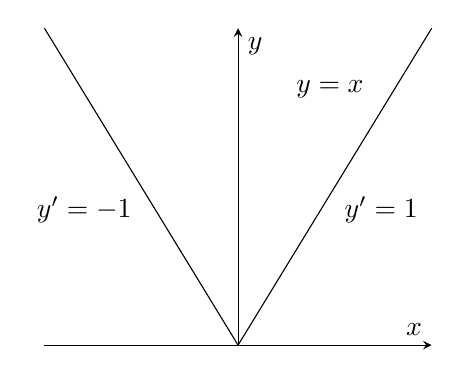
\begin{tikzpicture}
\begin{axis}[clip=false,small,axis lines=middle,xlabel={$x$},ylabel={$y$},xtick={\empty},ytick={\empty}]
\addplot[domain=-4:0]{-x}node[pos=0.5,below left]{$y'=-1$};
\addplot[domain=0:4]{x}node[pos=0.5,below right]{$y'=1$};
\draw(axis cs:1,3)node[above right]{$y=\abs{x}$};
\end{axis}
\end{tikzpicture}
\caption{چونکہ مبدا پر بائیں ہاتھ اور دائیں ہاتھ تفرق مختلف ہیں لہٰذا مبدا پر تفاعل کا تفرق غیر موجود ہے (مثال \حوالہ{مثال_تفرق_مبدا_پر_غیر_موجود})۔}
\label{شکل_مثال_تفرق_مبدا_پر_غیر_موجود}
\end{minipage}
\end{figure}

تفاعل کے دائرہ کار میں کہیں پر بھی تفاعل کے دائیں ہاتھ اور بائیں ہاتھ تفرق  معین ہو سکتے ہیں۔یک طرفہ اور دو طرفہ حد کا تعلق ان تفرق پر بھی قابل اطلاق ہو گا۔  مسئلہ \حوالہ{مسئلہ_حد_یک_طرفہ_بالمقابل_دو_طرفہ_حد} کی بنا کسی نقطے پر تفاعل کا تفرق صرف اور صرف اس صورت موجود ہو گا جب اس نقطے پر تفاعل کے بائیں ہاتھ تفرق اور دائیں ہاتھ تفرق موجود ہوں اور ایک دوسرے کے برابر ہوں۔

\ابتدا{مثال}\شناخت{مثال_تفرق_مبدا_پر_غیر_موجود}
تفاعل \عددی{y=\abs{x}} وقفہ \عددی{(-\infty,0)} اور \عددی{(0,\infty)} پر قابل تفرق ہے لیکن \عددی{x=0} پر اس کا تفرق موجود نہیں ہے۔مبدا کے دائیں جانب
\begin{align*}
\frac{\dif}{\dif x}(\abs{x})=\frac{\dif }{\dif x} (x)=\frac{\dif}{\dif x}(1\cdot x)=1,&& \tfrac{\dif}{\dif x}(mx+b)=m
\end{align*}
ہے جبکہ مبدا کے بائیں جانب
\begin{align*}
\frac{\dif}{\dif x}(\abs{x})=\frac{\dif }{\dif x} (-x)=\frac{\dif}{\dif x} (-1\cdot x)=-1
\end{align*}
ہے (شکل \حوالہ{شکل_مثال_تفرق_مبدا_پر_غیر_موجود})۔چونکہ مبدا پر تفاعل کا دائیں ہاتھ تفرق اور بائیں ہاتھ تفرق ایک جیسے نہیں ہیں لہٰذا مبدا پر تفاعل کا تفرق نہیں پایا جاتا ہے۔

صفر پر \عددی{\abs{x}} کا دائیں ہاتھ تفرق حاصل کرتے ہیں۔
\begin{align*}
\lim_{h\to 0^+}\frac{\abs{0+h}-\abs{0}}{h}&=\lim_{h\to 0^+}\frac{\abs{h}}{h}\quad\quad \text{\RL{اگر \عددی{h>0}  تب \عددی{\abs{h}=h} ہو گا}}\\
&=\lim_{h\to 0^+}\frac{h}{h}=\lim_{h\to 0^+} 1=1
\end{align*}
صفر پر \عددی{\abs{x}} کا بائیں ہاتھ تفرق حاصل کرتے ہیں۔
\begin{align*}
\lim_{h\to 0^-}\frac{\abs{0+h}-\abs{0}}{h}&=\lim_{h\to 0^-}\frac{\abs{h}}{h}\quad\quad \text{\RL{اگر \عددی{h<0}  تب \عددی{\abs{h}=-h} ہو گا}}\\
&=\lim_{h\to 0^-}\frac{-h}{h}=\lim_{h\to 0^-} -1=-1
\end{align*}
\انتہا{مثال}
%==========================

\جزوحصہء{کسی نقطے پر تفاعل کا تفرق کب نہیں پایا جاتا ہے؟}
اگر نقطہ \عددی{N(x_0,f(x_0))} اور اس کے قریب نقطہ \عددی{Q} سے گزرتے ہوئے سیکنٹ کی ڈھلوان، \عددی{Q} کو \عددی{N} کے نزدیک تر کرنے سے تحدیدی قیمت اختیار کرتی ہو  تب تفاعل \عددی{f(x)} نقطہ \عددی{N} پر قابل تفرق ہو گا۔اگر \عددی{Q} کو \عددی{N} کے نزدیک تر کرنے سے سیکنٹ کی ڈھلوان  تحدیدی قیمت اختیار نہ کرتی ہو یا یہ سیکنٹ انتصابی تحدیدی صورت اختیار کرتی ہو، تب اس تفاعل کا \عددی{N} پر تفرق نہیں پایا جائے گا۔ہموار منحنی والے تفاعل کا درج ذیل صورتوں میں نقطہ \عددی{N} پر تفرق نہیں پایا جائے گا۔
\begin{enumerate}[1.]

\item
نوکدار منحنی۔منحنی کی نوک  پر بائیں تفرق اور دائیں تفرق ایک جیسے نہیں ہوتے ہیں (شکل \حوالہ{شکل_تفرق_نا_قابل_نقطے}-ا)۔
\item
راس، جہاں \عددی{NQ} کی تحدیدی ڈھلوان ایک طرف سے \عددی{\infty} اور دوسری طرف سے \عددی{-\infty} ہوتی ہے (شکل \حوالہ{شکل_تفرق_نا_قابل_نقطے}-ب)۔ 
\item
انتصابی مماس، جہاں دونوں اطراف سے تحدیدی \عددی{NQ} کی ڈھلوان \عددی{\infty} یا \عددی{-\infty} ہوتی ہے (شکل \حوالہ{شکل_تفرق_نا_قابل_نقطے}-ج)۔
\item
عدم استمرار (شکل \حوالہ{شکل_تفرق_نا_قابل_نقطے}-د اور شکل \حوالہ{شکل_تفرق_نا_قابل_نقطے}-ہ)۔
\end{enumerate}

\begin{figure}
\centering
\begin{subfigure}{0.5\textwidth}
\centering
\begin{tikzpicture}
\draw[thick](0,0) to [out=45,in=-110]node[pos=0.2,left]{$Q^-$}coordinate[pos=0.2](kA)coordinate[pos=0.4](kB)coordinate[pos=0.6](kC)coordinate[pos=0.8](kD)coordinate[pos=0.95](kE)(1.5,2)node[shift={(-160:0.3)}]{$N$}coordinate(kN) to [out=-20,in=110]node[pos=0.8,left]{$Q^+$}coordinate[pos=0.8](kAA)coordinate[pos=0.6](kBB)coordinate[pos=0.4](kCC)coordinate[pos=0.2](kDD)coordinate[pos=0.05](kEE)(3,0);
\draw[gray,shorten <=-0.5cm, shorten >=-0.5cm] (kN)--(kA);
\draw[gray,shorten <=-0.5cm, shorten >=-1cm] (kN)--(kB);
\draw[gray,shorten <=-0.5cm, shorten >=-1.5cm] (kN)--(kC);
\draw[gray,shorten <=-0.5cm, shorten >=-2cm] (kN)--(kD);
\draw[shorten <=-0.5cm, shorten >=-2.5cm] (kN)--(kE);
%
\draw[gray,shorten <=-0.5cm, shorten >=-0.5cm] (kN)--(kAA);
\draw[gray,shorten <=-0.5cm, shorten >=-1cm] (kN)--(kBB);
\draw[gray,shorten <=-0.5cm, shorten >=-1.5cm] (kN)--(kCC);
\draw[gray,shorten <=-0.5cm, shorten >=-2cm] (kN)--(kDD);
\draw[shorten <=-0.5cm, shorten >=-2.5cm] (kN)--(kEE);
%
\draw(kA)node[circ]{} (kN)node[circ]{} (kAA)node[circ]{};
\end{tikzpicture}
\caption{نوک پر بائیں اور دائیں تفرق ایک دوسرے سے مختلف ہوتے ہیں۔}
\end{subfigure}%
\begin{subfigure}{0.5\textwidth}
\centering
\begin{tikzpicture}
\draw[thick](0,0) to [out=45,in=-90]node[pos=0.2,left]{$Q^-$}coordinate[pos=0.2](kA)coordinate[pos=0.4](kB)coordinate[pos=0.6](kC)coordinate[pos=0.8](kD)coordinate[pos=0.95](kE)(1.5,2)node[shift={(-160:0.3)}]{$N$}coordinate(kN) to [out=-90,in=135]node[pos=0.8,right,yshift=1mm]{$Q^+$}coordinate[pos=0.8](kAA)coordinate[pos=0.6](kBB)coordinate[pos=0.4](kCC)coordinate[pos=0.2](kDD)coordinate[pos=0.05](kEE)(3,0);
\draw[gray,shorten <=-0.5cm, shorten >=-0.5cm] (kN)--(kA);
\draw[gray,shorten <=-0.5cm, shorten >=-0.75cm] (kN)--(kB);
\draw[gray,shorten <=-0.5cm, shorten >=-1.25cm] (kN)--(kC);
\draw[gray,shorten <=-0.5cm, shorten >=-1.5cm] (kN)--(kD);
\draw[shorten <=-0.5cm, shorten >=-2cm] (kN)--(kE);
%
\draw[gray,shorten <=-0.5cm, shorten >=-0.5cm] (kN)--(kAA);
\draw[gray,shorten <=-0.5cm, shorten >=-0.75cm] (kN)--(kBB);
\draw[gray,shorten <=-0.5cm, shorten >=-1.25cm] (kN)--(kCC);
\draw[gray,shorten <=-0.5cm, shorten >=-1.5cm] (kN)--(kDD);
%
\draw(kA)node[circ]{} (kN)node[circ]{} (kAA)node[circ]{};
\end{tikzpicture}
\caption{راس پر ایک طرف سے ڈھلوان $\infty$ جبکہ دوسری طرف سے $-\infty$ ہوتی ہے۔}
\end{subfigure}
\begin{subfigure}{0.5\textwidth}
\centering
\begin{tikzpicture}
\draw[thick](0,0) to [out=-10,in=90]node[pos=0.2,left]{$Q^-$}coordinate[pos=0.2](kA)coordinate[pos=0.4](kB)coordinate[pos=0.6](kC)coordinate[pos=0.8](kD)coordinate[pos=0.95](kE)++(1.5,-1.5)node[shift={(-160:0.3)}]{$N$}coordinate(kN) to [out=-90,in=170]node[pos=0.8,right,yshift=1mm]{$Q^+$}coordinate[pos=0.8](kAA)coordinate[pos=0.6](kBB)coordinate[pos=0.4](kCC)coordinate[pos=0.2](kDD)coordinate[pos=0.05](kEE)++(1.5,-1.5);
\draw[gray,shorten <=-0.5cm, shorten >=-0.5cm] (kN)--(kA);
\draw[gray,shorten <=-0.5cm, shorten >=-0.75cm] (kN)--(kB);
\draw[gray,shorten <=-0.5cm, shorten >=-1cm] (kN)--(kC);
\draw[gray,shorten <=-0.5cm, shorten >=-1.25cm] (kN)--(kD);
%\draw[shorten <=-0.5cm, shorten >=-1.5cm] (kN)--(kE);
\draw[shorten <=-1.5cm](kN)--++(90:1.5);
%
\draw[gray,shorten <=-0.5cm, shorten >=-0.5cm] (kN)--(kAA);
\draw[gray,shorten <=-0.5cm, shorten >=-0.75cm] (kN)--(kBB);
\draw[gray,shorten <=-0.5cm, shorten >=-1cm] (kN)--(kCC);
\draw[gray,shorten <=-0.5cm, shorten >=-1.25cm] (kN)--(kDD);
%\draw[shorten <=-0.5cm, shorten >=-1.5cm] (kN)--(kEE);
%
\draw(kA)node[circ]{} (kN)node[circ]{} (kAA)node[circ]{};
\end{tikzpicture}
\caption{نقطہ $N$ پر مماس انتصابی ہے۔}
\end{subfigure}%
\begin{subfigure}{0.5\textwidth}
\centering
\begin{tikzpicture}
\draw[thick](0,0) to [out=10,in=-135]node[pos=0.2,shift={(135:0.3)}]{$Q^-$}coordinate[pos=0.2](kA)coordinate[pos=0.4](kB)coordinate[pos=0.6](kC)coordinate[pos=0.8](kD)coordinate[pos=1](kE)++(1.5,1) ++(0,1)node[shift={(-160:0.3)}]{$N$}coordinate(kN) to [out=-10,in=135]node[pos=0.8,left]{$Q^+$}coordinate[pos=0.8](kAA)coordinate[pos=0.6](kBB)coordinate[pos=0.4](kCC)coordinate[pos=0.2](kDD)coordinate[pos=0.05](kEE)++(1.5,-1.5);
\draw[gray,shorten <=-0.5cm, shorten >=-0.5cm] (kN)--(kA);
\draw[gray,shorten <=-0.5cm, shorten >=-0.5cm] (kN)--(kB);
\draw[gray,shorten <=-0.5cm, shorten >=-0.5cm] (kN)--(kC);
\draw[gray,shorten <=-0.5cm, shorten >=-0.75cm] (kN)--(kD);
\draw[shorten <=-0.5cm, shorten >=-1cm] (kN)--(kE);
%
\draw[gray,shorten <=-0.5cm, shorten >=-0.5cm] (kN)--(kAA);
\draw[gray,shorten <=-0.5cm, shorten >=-0.75cm] (kN)--(kBB);
\draw[gray,shorten <=-0.5cm, shorten >=-1cm] (kN)--(kCC);
\draw[gray,shorten <=-0.5cm, shorten >=-1.25cm] (kN)--(kDD);
\draw[shorten <=-0.5cm, shorten >=-1.5cm] (kN)--(kEE);
%
\draw(kA)node[circ]{} (kN)node[circ]{} (kAA)node[circ]{} (kE)node[ocirc]{};
\end{tikzpicture}
\caption{عدم استمرار}
\end{subfigure}
\begin{subfigure}{0.5\textwidth}
\centering
\begin{tikzpicture}
\draw[thick](0,0) to [out=-45,in=-180]node[pos=0.2,above]{$Q^-$}coordinate[pos=0.2](kA)coordinate[pos=0.4](kB)coordinate[pos=0.6](kC)coordinate[pos=0.8](kD)coordinate[pos=1](kE)++(1.5,-1)coordinate(kNN) to [out=0,in=135]node[pos=0.8,above right]{$Q^+$}coordinate[pos=0.8](kAA)coordinate[pos=0.6](kBB)coordinate[pos=0.4](kCC)coordinate[pos=0.2](kDD)coordinate[pos=0.05](kEE)++(1.5,-1);
\draw(kNN)++(0,1.5)coordinate(kN)node[right]{$N$};
\draw[gray,shorten <=-0.5cm, shorten >=-0.5cm] (kN)--(kA);
\draw[gray,shorten <=-0.5cm, shorten >=-0.5cm] (kN)--(kB);
\draw[gray,shorten <=-0.5cm, shorten >=-0.5cm] (kN)--(kC);
\draw[gray,shorten <=-0.5cm, shorten >=-0.75cm] (kN)--(kD);
\draw[shorten <=-0.5cm, shorten >=-1cm] (kN)--(kE);
%
\draw[gray,shorten <=-0.5cm, shorten >=-0.5cm] (kN)--(kAA);
\draw[gray,shorten <=-0.5cm, shorten >=-0.75cm] (kN)--(kBB);
\draw[gray,shorten <=-0.5cm, shorten >=-1cm] (kN)--(kCC);
\draw[gray,shorten <=-0.5cm, shorten >=-1.25cm] (kN)--(kDD);
%\draw[shorten <=-0.5cm, shorten >=-1.5cm] (kN)--(kEE);
%
\draw(kA)node[circ]{} (kN)node[circ]{} (kAA)node[circ]{} (kE)node[ocirc]{};
\end{tikzpicture}
\caption{عدم استمرار}
\end{subfigure}%
\caption{ان نقطوں کی پہچان جہاں تفاعل نا قابل تفرق ہو گا۔}
\label{شکل_تفرق_نا_قابل_نقطے}
\end{figure}

\جزوحصہء{قابل تفرق تفاعل استمراری ہوں گے}
جس نقطے پر ایک تفاعل قابل تفرق ہو اس پر یہ تفاعل استمراری ہو گا۔

\ابتدا{مسئلہ}\شناخت{مسئلہ_تفرق_قابل_تفرق_استمراری_ہے}
اگر \عددی{x=c} پر \عددی{f} کا تفرق موجود ہو تب \عددی{x=c} پر \عددی{f} استمراری ہو گا۔
\انتہا{مسئلہ}
%=========================
\ابتدا{ثبوت}
ہم جانتے ہیں کہ \عددی{f'(c)} موجود ہے اور ہم نے دکھانا ہے کہ \عددی{\lim_{x\to c}f(x)=f(c)} یا اس کا مماثل \عددی{\lim_{h\to 0}f(c+h)=f(c)} درست ہیں۔ اگر \عددی{h\ne 0} ہو تب درج ذیل ہو گا۔
\begin{align*}
f(c+h)&=f(c)+(f(c+h)-f(c))\\
&=f(c)+\frac{f(c+h)-f(c)}{h}\cdot h
\end{align*}
اب \عددی{h\to 0} لیں۔ مسئلہ \حوالہ{مسئلہ_حد_قواعد-الف} کے تحت درج ذیل ہو گا۔
\begin{align*}
\lim_{h\to 0}f(c+h)&=\lim_{h\to 0} f(c)+\lim_{h\to 0} \frac{f(c+h)-f(c)}{h}\cdot \lim_{h\to 0}h\\
&=f(c)+f'(c)\cdot 0\\
&=f(c)
\end{align*}
\انتہا{ثبوت}
%===========================

اسی قسم کی دلیل سے ثابت ہوتا ہے کہ اگر \عددی{x=c} پر \عددی{f} کا یک طرفہ (بایاں یا دایاں) تفرق پایا جاتا ہو تب \عددی{x=c} پر \عددی{f} اسی طرف (بائیں یا دائیں) سے استمراری ہو گا۔

\موٹا{انتباہ}\quad مسئلہ \حوالہ{مسئلہ_تفرق_قابل_تفرق_استمراری_ہے} کا الٹ درست نہیں ہے یعنی جس نقطے پر تفاعل استمراری ہو اس پر تفاعل نا قابل تفرق ہو سکتا ہے جیسے ہم نے مثال \حوالہ{مثال_تفرق_مبدا_پر_غیر_موجود} میں دیکھا۔

\موٹا{استمراری تفاعل کی ترسیم کتنی غیر ہموار ہو سکتی ہے؟} ہم نے دیکھا کہ مطلق قیمت تفاعل \عددی{y=\abs{x}} ایک نقطہ پر نا قابل تفرق ہوتا ہے۔یوں ہم استمراری دندان ترسیم (شکل \حوالہ{شکل_تفرق_دندان_ترسیم}) بنا سکتے ہیں جو لا متناہی تعداد کے نقطوں پر نا قابل تفرق ہو گا۔
\begin{figure}
\centering
\begin{minipage}{0.45\textwidth}
\centering
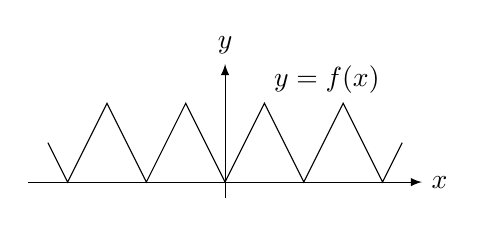
\begin{tikzpicture}[x=0.5cm]
\draw[-latex](-5,0)--(5,0)node[right]{$x$};
\draw[-latex](0,-0.2)--(0,1.5)node[above]{$y$};
\draw(0,0)--++(1,1)node[above right]{$y=f(x)$}--++(1,-1)--++(1,1)--++(1,-1)--++(0.5,0.5);
\draw(0,0)--++(-1,1)--++(-1,-1)--++(-1,1)--++(-1,-1)--++(-0.5,0.5);
\end{tikzpicture}
\caption{دندان ترسیم استمراری لیکن لا متناہی نقطوں پر نا قابل تفرق ہے۔}
\label{شکل_تفرق_دندان_ترسیم}
\end{minipage}\hfill
\begin{minipage}{0.45\textwidth}
\centering
\begin{tikzpicture}
\draw[-latex](-2,0)--(2,0)node[right]{$x$};
\draw[-latex](0,-0.2)--(0,1.5)node[above]{$y$};
\draw[thick](-2,0)--(0,0)node[ocirc]{} (0,1)node[circ]{}--(2,1)node[pos=0.75,above]{$y=\cup(x)$};
\end{tikzpicture}
\caption{اکائی سیڑھی تفاعل متوسط قیمت خاصیت نہیں رکھتا ہے لہٰذا حقیقی خط پر یہ کسی دوسرے تفاعل کا تفرق نہیں ہو سکتا ہے۔}
\label{شکل_تفرق_اکائی_سیڑھی_تفاعل}
\end{minipage}
\end{figure}

\موٹا{کیا استمراری تفاعل ہر نقطے پر نا قابل تفرق ہو سکتا ہے؟} اس کا جواب ہے "جی ہاں" جیسے  \ترچھا{کارل وائشسٹراس}\حاشیہب{جرمن ریاضی دان کارل وائشسٹراس [1815-1897]} نے \سن{1872} میں درج ذیل کلیہ (اور کئی اور) پیش کرتے ہوئے ثابت کیا۔
\begin{align*}
f(x)=\sum_{n=0}^{\infty}\big(\frac{2}{3}\big)^n\cos (9^n\pi x)
\end{align*}
یہ کلیہ \عددی{f} کو  بڑھتی تعدد کے کوسائن تفاعل کے مجموعے کی صورت میں پیش کرتا ہے۔بل کو بل دینے سے ایسا تفاعل حاصل ہوتا ہے جس کا تحدیدی سیکنٹ کسی بھی نقطے پر حاصل کرنا ممکن نہیں ہوتا ہے لہٰذا اس کا مماس کہیں پر بھی نہیں پایا جاتا ہے۔ 

استمراری تفاعل جن کا کسی بھی نقطے پر مماس نہ پایا جاتا ہو \ترچھا{نظریہ ابتری}\فرہنگ{نظریہ!ابتری}\حاشیہب{chaos theory}\فرہنگ{chaos theory} میں کلیدی کردار ادا کرتے ہیں۔ ایسے تفاعل کو متناہی لمبائی مختص کرنا ممکن نہیں ہوتا ہے۔ہم منحنی کی لمبائی اور تفرق کا تعلق پر بعد میں غور کریں گے۔

\جزوحصہء{تفرق کی متوسط قیمت خاصیت}
ضروری نہیں ہے کہ ایک تفاعل کسی دوسرے کا تفرقی تفاعل ہو۔درج ذیل مسئلہ سے اس حقیقت کو اخذ کیا جا سکتا ہے۔

\ابتدا{مسئلہ}\شناخت{مسئلہ_تفرق_متوسط_قیمت_خاصیت}
اگر جس وقفے پر \عددی{f} قابل تفرق ہو اس وقفے میں نقطہ \عددی{a} اور \عددی{b} پائے جاتے ہیں تب  \عددی{f'(a)} اور \عددی{f'(b)} کے بیچ ہر قیمت کا تفرق \عددی{f'} پایا جائے گا۔ 
\انتہا{مسئلہ}
%===========================

مسئلہ \حوالہ{مسئلہ_تفرق_متوسط_قیمت_خاصیت} (جس کا ثبوت ہم پیش نہیں کریں گے)  کہتا ہے کہ کسی وقفے پر ایک تفاعل اس صورت تک کسی دوسرے تفاعل کا تفرق نہیں ہو گا جب تک اس وقفے پر یہ متوسط قیمت خاصیت نہ رکھتا ہو (شکل \حوالہ{شکل_تفرق_اکائی_سیڑھی_تفاعل})۔ ایک تفاعل کب کسی دوسرے تفاعل کا تفرق ہو گا؟ یہ احصاء کی اہم ترین سوالات میں سے ایک ہے جس کا جواب نیوٹن اور لیبنٹز نے دے کر ریاضیات میں انقلاب برپا کیا۔ان کے جواب کو ہم باب \حوالہ{باب_تکمل} میں دیکھیں گے۔

\حصہء{سوالات}
\موٹا{تفرقی تفاعل اور قیمتوں کی تلاش}\\
سوال \حوالہ{سوال_تفرق_قیمت_تلاش_الف} تا سوال \حوالہ{سوال_تفرق_قیمت_تلاش_ب} میں تفرق کی تعریف استعمال کرتے ہوئے دیے گئے تفاعل کے تفرق کی قیمت تلاش کریں۔  

\ابتدا{سوال}\شناخت{سوال_تفرق_قیمت_تلاش_الف}\quad
$f(x)=4-x^2; \quad f'(-3), f'(0), f'(1)$\\
جواب:\quad
$-2x,6,0,-2$
\انتہا{سوال}
%==================
\ابتدا{سوال}
$F(x)=(x-1)^2+1;\quad F'(-1), F'(0), F'(2)$
\انتہا{سوال}
%====================
\ابتدا{سوال}
$g(t)=\tfrac{1}{t^2};\quad g'(-1), g'(2), g'(\sqrt{3})$\\
جواب:\quad
$-\tfrac{2}{t^3},2,-\tfrac{1}{4},-\tfrac{2}{3\sqrt{3}}$
\انتہا{سوال}
%====================
\ابتدا{سوال}
$k(z)=\tfrac{1-z}{2z};\quad k'(-1), k'(1), k'(\sqrt{2})$
\انتہا{سوال}
%====================
\ابتدا{سوال}
$p(\theta)=\sqrt{3\theta};\quad p'(1), p'(3), p'(\tfrac{2}{3})$\\
جواب:\quad
$\tfrac{3}{2\sqrt{3\theta}},\tfrac{3}{2\sqrt{3}},\tfrac{1}{2},\tfrac{3}{2\sqrt{2}}$
\انتہا{سوال}
%====================
\ابتدا{سوال}\شناخت{سوال_تفرق_قیمت_تلاش_ب}\quad
$r(s)=\sqrt{2s+1};\quad r'(0), r'(1), r'(\tfrac{1}{2})$
\انتہا{سوال}
%====================
سوال \حوالہ{سوال_تفرق_درکار_حاصل_الف} تا سوال \حوالہ{سوال_تفرق_درکار_حاصل_ب} میں دیا گیا تفرق حاصل کریں۔

\ابتدا{سوال}\شناخت{سوال_تفرق_درکار_حاصل_الف}
$y=2x^3;\quad \tfrac{\dif y}{\dif x}$\\
جواب:\quad
$6x^2$
\انتہا{سوال}
%========================
\ابتدا{سوال}
$r=\tfrac{s^3}{2}+1;\quad \tfrac{\dif r}{\dif s}$
\انتہا{سوال}
%========================
\ابتدا{سوال}
$s=\tfrac{t}{2t+1};\quad \tfrac{\dif s}{\dif t}$\\
جواب:\quad
$\tfrac{1}{(2t+1)^2}$
\انتہا{سوال}
%========================
\ابتدا{سوال}
$v=t-\tfrac{1}{t};\quad \tfrac{\dif v}{\dif t}$
\انتہا{سوال}
%========================
\ابتدا{سوال}
$p=\tfrac{1}{\sqrt{q+1}};\quad \tfrac{\dif p}{\dif q}$\\
جواب:\quad
 $-\tfrac{1}{2(q+1)\sqrt{q+1}}$
\انتہا{سوال}
%========================
\ابتدا{سوال}\شناخت{سوال_تفرق_درکار_حاصل_ب}
$z=\tfrac{1}{\sqrt{3w-2}};\quad \tfrac{\dif z}{\dif w}$
\انتہا{سوال}
%========================
\موٹا{ڈھلوان اور مماسی خطوط}\\
سوال \حوالہ{سوال_تفرق_ڈھلوان_تلاش_الف} تا سوال \حوالہ{سوال_تفرق_ڈھلوان_تلاش_ب} میں تفاعل کا تفرق حاصل کرتے ہوئے دیے گئے غیر تابع متغیر پر مماس کی ڈھلوان تلاش کریں۔

\ابتدا{سوال}\شناخت{سوال_تفرق_ڈھلوان_تلاش_الف}
$f(x)=x+\tfrac{9}{x};\quad x=-3$\\
جواب:\quad
$1-\tfrac{9}{x^2},0$
\انتہا{سوال}
%=====================
\ابتدا{سوال}
$k(x)=\tfrac{1}{2+x};\quad x=2$
\انتہا{سوال}
%=====================
\ابتدا{سوال}
$s=t^3-t^2;\quad t=-1$\\
جواب:\quad
$3t^2-2t,5$
\انتہا{سوال}
%=====================
\ابتدا{سوال}\شناخت{سوال_تفرق_ڈھلوان_تلاش_ب}
$y=(x+1)^3;\quad x=-2$
\انتہا{سوال}
%=====================
سوال \حوالہ{سوال_تفرق_مماس_مساوات_الف} تا سوال \حوالہ{سوال_تفرق_مماس_مساوات_ب} میں تفاعل کا تفرق حاصل کریں۔ ترسیم پر دیے گئے نقطے پہ تفاعل کے مماس کی مساوات تلاش کریں۔

\ابتدا{سوال}\شناخت{سوال_تفرق_مماس_مساوات_الف}
$f(x)=\tfrac{8}{\sqrt{x-2}};\quad (x,y)=(6,4)$\\
جواب:\quad
$\tfrac{-4}{(x-2)\sqrt{x-2}},y-4=-\tfrac{1}{2}(x-6)$
\انتہا{سوال}
%======================
\ابتدا{سوال}\شناخت{سوال_تفرق_مماس_مساوات_ب}
$g(z)=1+\sqrt{4-z};\quad (z,w)=(3,2)$
\انتہا{سوال}
%======================
سوال \حوالہ{سوال_تفرق_قیمت_نقطے_پر_تلاش_الف} تا سوال \حوالہ{سوال_تفرق_قیمت_نقطے_پر_تلاش_ب} میں تفرق کی قیمت تلاش کریں۔

\ابتدا{سوال}\شناخت{سوال_تفرق_قیمت_نقطے_پر_تلاش_الف}
$\left. \tfrac{\dif s}{\dif t}\right\vert_{t=-1};\quad s=1-3t^2$\\
جواب:\quad
$6$
\انتہا{سوال}
%======================
\ابتدا{سوال}
$\left. \tfrac{\dif y}{\dif x}\right\vert_{x=\sqrt{3}};\quad y=1-\tfrac{1}{x}$
\انتہا{سوال}
%======================
\ابتدا{سوال}
$\left. \tfrac{\dif r}{\dif \theta}\right\vert_{\theta=0};\quad r=\tfrac{2}{\sqrt{4-\theta}}$\\
جواب:\quad
$\tfrac{1}{8}$
\انتہا{سوال}
%======================
\ابتدا{سوال}\شناخت{سوال_تفرق_قیمت_نقطے_پر_تلاش_ب}
$\left. \tfrac{\dif w}{\dif z}\right\vert_{z=4};\quad w=z+\sqrt{z}$
\انتہا{سوال}
%======================
\موٹا{تفرق کے حصول کا متبادل کلیہ}\\
تحدیدی سیکنٹ سے تفرق کا حاصل کلیہ مستعمل نقطوں کی علامتی اظہار پر منحصر ہوتا ہے۔شکل \حوالہ{شکل_تفرق_متبادل_طریقہ} میں سیکنٹ کی ڈھلوان \عددی{\tfrac{f(x)-f(c)}{x-c}} ہے جس کی \عددی{N} پر  تحدیدی قیمت (\عددی{Q} کو \عددی{N} کے نزدیک تر کرتے ہوئے) \عددی{N} پر تفاعل کا تفرق دیتی ہے۔
\begin{align}\label{مساوات_تفرق_متبادل_کلیہ}
f'(c)=\lim_{x\to c} \frac{f(x)-f(c)}{x-c}
\end{align}
%
\begin{figure}
\centering
\begin{tikzpicture}[font=\small,declare function={f(\x)=2-sin(\x);}]
\pgfmathsetmacro{\kS}{70}
\pgfmathsetmacro{\kE}{260}
\pgfmathsetmacro{\kN}{\kS+0.1*(\kE-\kS)}
\pgfmathsetmacro{\kQ}{\kS+0.7*(\kE-\kS)}
\draw(0,0)--(5,0);
\draw[domain=\kS:\kE] plot ({\x*pi/180},{f(\x)})node[above]{$y=f(x)$};
\draw[shorten <=-0.5cm, shorten >=-0.5cm] ({\kN*pi/180},{f(\kN)})node[circ]{}coordinate(kA)node[above,xshift=-2mm,yshift=2mm]{$N(c,f(c))$}--({\kQ*pi/180},{f(\kQ)})node[circ]{}coordinate(kB)node[left,yshift=2mm]{$Q(x,f(x))$};
\draw[dashed](kA)--($(0,0)!(kA)!(5,0)$)node[circ]{}node[below]{$c$}coordinate[pos=0.4](kL);
\path[name path=kR](kB)--($(0,0)!(kB)!(5,0)$);
\path[name path=kH](kA)--++(5,0);
\draw[name intersections={of={kH and kR}}] (kA)--(intersection-1)--(kB);
\draw[dashed] (intersection-1)--($(0,0)!(intersection-1)!(5,0)$)node[circ]{}node[below]{$x$}coordinate(kRB);
\draw[stealth-stealth](kL)--($(intersection-1)!(kL)!(kRB)$)node[pos=0.5,fill=white]{$h=x-c$};
\draw(kB)++(0.3,0)--++(0.3,0)coordinate[pos=0.5](kTop);
\draw(intersection-1)++(0.3,0)--++(0.3,0)coordinate[pos=0.5](kBot);
\draw[stealth-stealth](kTop)--(kBot)node[pos=0.5,right]{$f(x)-f(c)$};
\end{tikzpicture}
\caption{حصول تفرق کا متبادل کلیہ}
\label{شکل_تفرق_متبادل_طریقہ}
\end{figure} 

اس کلیہ کا استعمال چند تفرق کا حصول آسان بناتا ہے۔سوال \حوالہ{سوال_تفرق_متبادل_الف} تا سوال \حوالہ{سوال_تفرق_متبادل_ب} میں اس کلیہ کی مدد سے \عددی{c} پر تفاعل کا تفرق حاصل کریں۔  

\ابتدا{سوال}\شناخت{سوال_تفرق_متبادل_الف}
$f(x)=\tfrac{1}{x+2},\quad c=-1$\\
جواب:\quad
$-1$
\انتہا{سوال}
%=====================
\ابتدا{سوال}
$f(x)=\tfrac{1}{(x-1)^2},\quad c=2$
\انتہا{سوال}
%=====================
\ابتدا{سوال}
$g(t)=\tfrac{t}{t-1},\quad c=3$\\
جواب:\quad
$-\tfrac{1}{4}$
\انتہا{سوال}
%=====================
\ابتدا{سوال}\شناخت{سوال_تفرق_متبادل_ب}
$k(s)=1+\sqrt{s},\quad c=9$
\انتہا{سوال}
%=====================
\موٹا{ترسیمات}
سوال \حوالہ{سوال_شکل_تفرق_اصل_تلاش_الف} تا سوال \حوالہ{سوال_شکل_تفرق_اصل_تلاش_ب} میں دیے گئے تفاعل کا تفرق شکل \حوالہ{شکل_تفرق_اصل_تلاش} میں تلاش کریں۔
\begin{figure}
\centering
\begin{minipage}{1\textwidth}
\begin{subfigure}{0.25\textwidth}
\centering
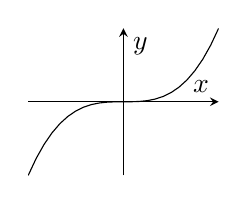
\begin{tikzpicture}[]
\begin{axis}[small,width=4cm,axis lines=middle,xlabel={$x$},ylabel={$y$},xtick={\empty},ytick={\empty}]
\addplot[domain=-2:2]{x^3};
\end{axis}
\end{tikzpicture}
\caption{}
\end{subfigure}%
\begin{subfigure}{0.25\textwidth}
\centering
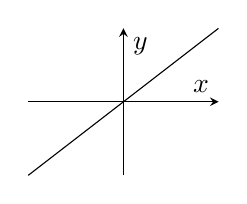
\begin{tikzpicture}[]
\begin{axis}[small,width=4cm,axis lines=middle,xlabel={$x$},ylabel={$y$},xtick={\empty},ytick={\empty}]
\addplot[domain=-2:2]{x};
\end{axis}
\end{tikzpicture}
\caption{}
\end{subfigure}%
\begin{subfigure}{0.25\textwidth}
\centering
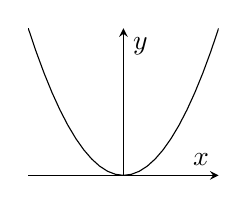
\begin{tikzpicture}[]
\begin{axis}[small,width=4cm,axis lines=middle,xlabel={$x$},ylabel={$y$},xtick={\empty},ytick={\empty}]
\addplot[domain=-2:2]{x^2};
\end{axis}
\end{tikzpicture}
\caption{}
\end{subfigure}%
\begin{subfigure}{0.25\textwidth}
\centering
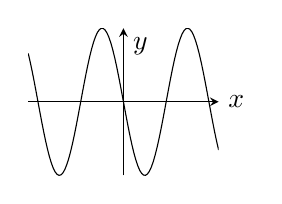
\begin{tikzpicture}[]
\begin{axis}[small,width=4cm,axis lines=middle,xlabel={$x$},ylabel={$y$},xtick={\empty},ytick={\empty},xlabel style={at={(current axis.right of origin)},anchor=west}]
\addplot[domain=-7:7,samples=100]{-sin(deg(x))};
\end{axis}
\end{tikzpicture}
\caption{}
\end{subfigure}
\caption{تفاعل کے تفرق}
\label{شکل_تفرق_اصل_تلاش}
\end{minipage}
\begin{minipage}{1\textwidth}
\begin{subfigure}{0.25\textwidth}
\centering
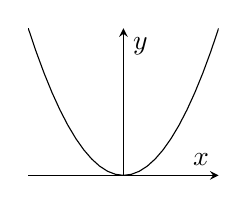
\begin{tikzpicture}[]
\begin{axis}[small,width=4cm,axis lines=middle,xlabel={$x$},ylabel={$y$},xtick={\empty},ytick={\empty}]
\addplot[domain=-2:2]{1/2*x^2};
\end{axis}
\end{tikzpicture}
\caption{}
\end{subfigure}%
\begin{subfigure}{0.25\textwidth}
\centering
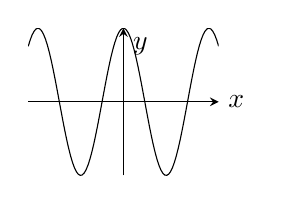
\begin{tikzpicture}[]
\begin{axis}[small,width=4cm,axis lines=middle,xlabel={$x$},ylabel={$y$},xtick={\empty},ytick={\empty},xlabel style={at={(current axis.right of origin)},anchor=west}]
\addplot[domain=-7:7,samples=100]{cos(deg(x))};
\end{axis}
\end{tikzpicture}
\caption{}
\end{subfigure}%
\begin{subfigure}{0.25\textwidth}
\centering
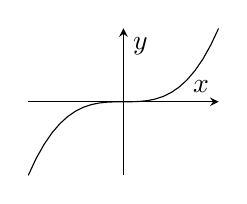
\begin{tikzpicture}[]
\begin{axis}[small,width=4cm,axis lines=middle,xlabel={$x$},ylabel={$y$},xtick={\empty},ytick={\empty}]
\addplot[domain=-2:2]{1/3*x^3};
\end{axis}
\end{tikzpicture}
\caption{}
\end{subfigure}%
\begin{subfigure}{0.25\textwidth}
\centering
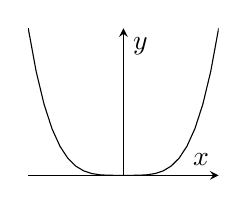
\begin{tikzpicture}[]
\begin{axis}[small,width=4cm,axis lines=middle,xlabel={$x$},ylabel={$y$},xtick={\empty},ytick={\empty}]
\addplot[domain=-1:1]{1/4*x^4};
\end{axis}
\end{tikzpicture}
\caption{}
\end{subfigure}%
\caption{اصل تفاعل}
\label{شکل_تفرق_اصل}
\end{minipage}
\end{figure}

\ابتدا{سوال}\شناخت{سوال_شکل_تفرق_اصل_تلاش_الف}
شکل \حوالہ{شکل_تفرق_اصل}-ا\\
جواب:\quad
شکل \حوالہ{شکل_تفرق_اصل_تلاش}-ب
\انتہا{سوال}
%==============================
\ابتدا{سوال}
شکل \حوالہ{شکل_تفرق_اصل}-ب\\
جواب:\quad
شکل \حوالہ{شکل_تفرق_اصل_تلاش}-د
\انتہا{سوال}
%==============================
\ابتدا{سوال}
شکل \حوالہ{شکل_تفرق_اصل}-ج\\
جواب:\quad
شکل \حوالہ{شکل_تفرق_اصل_تلاش}-ج
\انتہا{سوال}
%==============================
\ابتدا{سوال}\شناخت{سوال_شکل_تفرق_اصل_تلاش_ب}
شکل \حوالہ{شکل_تفرق_اصل}-د\\
جواب:\quad
شکل \حوالہ{شکل_تفرق_اصل_تلاش}-ا
\انتہا{سوال}
%==============================
\ابتدا{سوال}\شناخت{سوال_تفرق_کیا_موجود_الف}
قطعات کو جوڑ کر شکل \حوالہ{شکل_سوال_تفرق_کیا_موجود_الف} حاصل کی گئی ہے۔(ا) وقفہ \عددی{[-4,6]} پر کہاں \عددی{f'} غیر معین ہو گا؟ اپنے جواب کی وجہ پیش کریں۔ (ب) انتصابی محور کو \عددی{y'} کہتے ہوئے \عددی{f'} کو ترسیم کریں۔ترسیم سیڑھی نما ہو گا۔
\begin{figure}
\centering
\begin{minipage}{0.45\textwidth}
\begin{tikzpicture}
\begin{axis}[small,axis lines=middle,xlabel={$x$},ylabel={$y$},xmin=-6,xmax=7.5,ymin=-3,ymax=3,xtick={1,6},ytick={\empty}]
\addplot[] plot coordinates {(-4,0) (0,2) (1,-2) (4,-2) (6,2)};
\draw(axis cs:-4,0)node[circ]{}node[below]{$(-4,0)$}  (axis cs:0,2)node[circ]{}node[left]{$(0,2)$} (axis cs:1,-2)node[circ]{}node[below]{$(1,-2)$}  (axis cs:4,-2)node[circ]{}node[right]{$(4,-2)$} (axis cs:6,2)node[circ]{}node[above]{$(6,2)$} (axis cs:3,1.5)node[]{$y=f(x)$};
\end{axis}
\end{tikzpicture}
\caption{ترسیم برائے سوال \حوالہ{سوال_تفرق_کیا_موجود_الف}}
\label{شکل_سوال_تفرق_کیا_موجود_الف}
\end{minipage}\hfill
\begin{minipage}{0.45\textwidth}
\begin{tikzpicture}
\begin{axis}[small,axis lines=middle,xlabel={$x$},ylabel={$y'$},xmin=-6,xmax=7.5,ymin=-3,ymax=3,xtick={-2,1,3,5},ytick={1}]
\draw[thick](axis cs:-2,-2)node[circ]{}--(axis cs:0,-2)node[ocirc]{}node[right]{$-2$} (axis cs:0,0)node[ocirc]{}--(axis cs:1,0)node[ocirc]{} (axis cs:1,1)node[ocirc]{}--(axis cs:3,1)node[ocirc]{} (axis cs:3,-1)node[ocirc]{}--(axis cs:5,-1)node[circ]{} (axis cs:3,2)node[right]{$y=f'(x)$};
\end{axis}
\end{tikzpicture}
\caption{تفاعل کے تفرق کا ترسیم برائے سوال \حوالہ{سوال_تفرق_سے_اصل_کا_حصول}}
\label{شکل_سوال_تفرق_سے_اصل_کا_حصول}
\end{minipage}
\end{figure}

جواب:\quad
(ا) \عددی{x=0,1,4}؛ (ب) شکل \حوالہ{شکل_سوال_تفرق_کیا_موجود_الف_جواب}
\begin{figure}
\centering
\begin{minipage}{0.45\textwidth}
\centering
\begin{tikzpicture}
\begin{axis}[small,axis lines=middle,xlabel={$x$},ylabel={$y'$},xmin=-5,xmax=7,ymin=-5,ymax=3,ytick={-4,1,2}]
\draw[thick](axis cs:-4,0.5)node[ocirc]{}--(axis cs:0,0.5)node[ocirc]{} (axis cs:0,-4)node[ocirc]{}--(axis cs:1,-4)node[ocirc]{} (axis cs:1,0)node[ocirc]{}--(axis cs:4,0)node[ocirc]{} (axis cs:4,2)node[ocirc]{}--(axis cs:6,2)node[ocirc]{};
\end{axis}
\end{tikzpicture}
\caption{جواب برائے سوال \حوالہ{سوال_تفرق_سے_اصل_کا_حصول}}
\label{شکل_سوال_تفرق_کیا_موجود_الف_جواب}
\end{minipage}
\end{figure}
\انتہا{سوال}
%============================
\ابتدا{سوال}\شناخت{سوال_تفرق_سے_اصل_کا_حصول}\ترچھا{تفاعل کے تفرق سے اصل تفرق کی وصولی}\\
(ا) \quad
درج ذیل طریقے سے تفاعل \عددی{f} ترسیم کو وقفہ \عددی{[-2,5]} پر کریں۔
\begin{enumerate}[1.]

\item
بند قطعات کو جوڑ کر ترسیم حاصل کریں۔
\item
ترسیم کو نقطہ \عددی{(-2,3)} سے شروع کریں۔
\item
تفاعل کا تفرق شکل \حوالہ{شکل_سوال_تفرق_سے_اصل_کا_حصول} میں دکھایا گیا ہے۔
\end{enumerate}
(ب)\quad
نقطہ \عددی{(-2,0)} سے شروع کرتے ہوئے جزو (ا) کا ترسیم دوبارہ حاصل کریں۔
\انتہا{سوال}
%======================
سوال \حوالہ{سوال_تفرق_نا_قابل_الف} تا سوال \حوالہ{سوال_تفرق_نا_قابل_د} میں نقطہ \عددی{N} پر بائیں اور دائیں ہاتھ تفرق کا موازنہ کرتے ہوئے دکھائیں کہ اس نقطے پر تفاعل نا قابل تفرق ہے۔

\ابتدا{سوال}\شناخت{سوال_تفرق_نا_قابل_الف}
تفاعل کو شکل  \حوالہ{شکل_سوال_تفرق_نا_قابل_الف} میں دکھایا گیا ہے۔\\
جواب:\quad
چونکہ \عددی{\lim_{x\to 0^+}f'(x)=1} جبکہ \عددی{\lim_{x\to 0^-}f'(x)=0} ہے لہٰذا \عددی{x=0} پر \عددی{f(x)} نا قابل تفرق ہے۔
 \begin{figure}
\centering
\begin{minipage}{0.25\textwidth}
\centering
\begin{tikzpicture}
\begin{axis}[clip=false,small,width=4cm,axis lines=middle,xlabel={$x$},ylabel={$y$},xtick={\empty},ytick={\empty},ymin=-0.5,font=\footnotesize,ylabel style={at={(current axis.above origin)},anchor=south},xlabel style={at={(current axis.right of origin)},anchor=west}]
\addplot[domain=-1.4142:0]{x^2}node[pos=0.5,fill=white]{$y=x^2$};
\addplot[domain=0:2]{x}node[pos=0.5,fill=white]{$y=x$};
\draw(axis cs:0,0)node[circ]{}node[below right]{$N(0,0)$};
\draw(axis cs:0,2)node[right]{$y=f(x)$};
\end{axis}
\end{tikzpicture}
\caption{}
\label{شکل_سوال_تفرق_نا_قابل_الف}
\end{minipage}\hfill
\begin{minipage}{0.25\textwidth}
\centering
\begin{tikzpicture}
\begin{axis}[clip=false,small,width=4cm,axis lines=middle,xlabel={$x$},ylabel={$y$},xtick={\empty},ytick={\empty},ymin=-0.5,font=\footnotesize,ylabel style={at={(current axis.above origin)},anchor=south},xtick={1,2},ytick={1,3},xmax=3,xlabel style={at={(current axis.right of origin)},anchor=west}]
\addplot[] plot coordinates {(-2,2) (1,2)};
\addplot[domain=1:2]{2*x}node[pos=0.5,right]{$y=2x$};
\draw(axis cs:1,2)node[circ]{}node[below right]{$N(1,2)$};
\draw(axis cs:0,4)node[left]{$y=f(x)$};
\draw(axis cs:-2,2)node[above]{$y=2$};
\end{axis}
\end{tikzpicture}
\caption{}
\label{شکل_سوال_تفرق_نا_قابل_ب}
\end{minipage}\hfill
\begin{minipage}{0.25\textwidth}
\centering
\begin{tikzpicture}
\begin{axis}[clip=false,small,width=4cm,axis lines=middle,xlabel={$x$},ylabel={$y$},xtick={\empty},ytick={\empty},ymin=-0.5,font=\footnotesize,ylabel style={at={(current axis.above origin)},anchor=south},xtick={1},ytick={1},xmax=3,xlabel style={at={(current axis.right of origin)},anchor=west}]
\addplot[domain=0:1]{sqrt(x)}node[pos=0.3,right]{$y=\sqrt{x}$};
\addplot[domain=1:2]{2*x-1}node[pos=0.5,fill=white]{$y=2x-1$};
\draw(axis cs:1,1)node[circ]{}node[right]{$N(1,1)$};
\draw(axis cs:0,3)node[right]{$y=f(x)$};
\end{axis}
\end{tikzpicture}
\caption{}
\label{شکل_سوال_تفرق_نا_قابل_ج}
\end{minipage}\hfill
\begin{minipage}{0.25\textwidth}
\centering
\begin{tikzpicture}
\begin{axis}[clip=false,small,width=4cm,axis lines=middle,xlabel={$x$},ylabel={$y$},xtick={\empty},ytick={\empty},ymin=-0.5,font=\footnotesize,ylabel style={at={(current axis.above origin)},anchor=south},xtick={1},ytick={1},xmax=3,ymax=2,xlabel style={at={(current axis.right of origin)},anchor=west}]
\addplot[domain=-1:1]{x}node[pos=0.15,right]{$y=x$};
\addplot[domain=1:2.5]{1/x}node[pos=0.5,above right]{$y=\tfrac{1}{x}$};
\draw(axis cs:1,1)node[circ]{}node[above]{$N(1,1)$};
\draw(axis cs:0,2)node[right]{$y=f(x)$};
\end{axis}
\end{tikzpicture}
\caption{}
\label{شکل_سوال_تفرق_نا_قابل_د}
\end{minipage}%
\end{figure}
\انتہا{سوال}
%======================
\ابتدا{سوال}\شناخت{سوال_تفرق_نا_قابل_ب}
تفاعل کو شکل  \حوالہ{شکل_سوال_تفرق_نا_قابل_ب} میں دکھایا گیا ہے۔
\انتہا{سوال}
%===========================
\ابتدا{سوال}\شناخت{سوال_تفرق_نا_قابل_ج}
تفاعل کو شکل  \حوالہ{شکل_سوال_تفرق_نا_قابل_ج} میں دکھایا گیا ہے۔\\
جواب:\quad
چونکہ \عددی{\lim_{x\to 1^+}f'(x)=2} جبکہ \عددی{\lim_{x\to 1^-}f'(x)=\tfrac{1}{2}} ہے لہٰذا \عددی{x=1} پر \عددی{f(x)} نا قابل تفرق ہے۔
\انتہا{سوال}
%===========================
\ابتدا{سوال}\شناخت{سوال_تفرق_نا_قابل_د}
تفاعل کو شکل  \حوالہ{شکل_سوال_تفرق_نا_قابل_د} میں دکھایا گیا ہے۔
\انتہا{سوال}
%===========================
سوال \حوالہ{سوال_تفرق_کیا_ہے_الف} تا سوال \حوالہ{سوال_تفرق_کیا_ہے_و} میں بند دائرہ کار \عددی{D} پر تفاعل کا ترسیم دکھایا گیا ہے۔کن نقطوں پر تفاعل (ا) قابل تفرق، (ب) استمراری لیکن نا قابل تفرق، (ج) غیر استمراری اور نا قابل تفرق ہے؟

\ابتدا{سوال}\شناخت{سوال_تفرق_کیا_ہے_الف}
ترسیم شکل \حوالہ{شکل_سوال_تفرق_کیا_ہے_الف} میں دکھایا گیا ہے جبکہ \عددی{D:-3\le x\le 2} ہے۔
\begin{figure}
\centering
\begin{minipage}{0.3\textwidth}
\centering
\begin{tikzpicture}
\begin{axis}[clip=false,small,width=4cm,axis lines=middle,xlabel={$x$},ylabel={$y$},xtick={\empty},ytick={\empty},ymin=-0.5,font=\footnotesize,ylabel style={at={(current axis.above origin)},anchor=south},xtick={-3,-2,1,2},ytick={-2,1,2}, xmin=-3.5, xmax=2.5,ymin=-2.5, ymax=2.5,xlabel style={at={(current axis.right of origin)},anchor=west}]
\draw(axis cs:-3,2)node[circ]{}--(axis cs:2,-2)node[circ]{};
\draw(axis cs:0,1.5)node[right]{$y=f(x)$};
\end{axis}
\end{tikzpicture}
\caption{}
\label{شکل_سوال_تفرق_کیا_ہے_الف}
\end{minipage}\hfill
\begin{minipage}{0.3\textwidth}
\centering
\begin{tikzpicture}
\begin{axis}[clip=false,small,width=4cm,axis lines=middle,xlabel={$x$},ylabel={$y$},xtick={\empty},ytick={\empty},ymin=-0.5,font=\footnotesize,ylabel style={at={(current axis.above origin)},anchor=south},xtick={-3,6},xticklabels={$-2$,$3$},ytick={\empty},xlabel style={at={(current axis.right of origin)},anchor=west},xmin=-4,xmax=7]
\addplot[domain=-3:6,samples=100]{e^(-0.1*x)*sin(deg(x+3))}node[pos=0,circ]{}node[pos=1,circ]{};
\draw(axis cs:0,1)node[right]{$y=f(x)$};
\end{axis}
\end{tikzpicture}
\caption{}
\label{شکل_سوال_تفرق_کیا_ہے_ب}
\end{minipage}\hfill
\begin{minipage}{0.3\textwidth}
\centering
\begin{tikzpicture}
\begin{axis}[clip=false,small,width=4cm,axis lines=middle,xlabel={$x$},ylabel={$y$},xtick={\empty},ytick={\empty},ymin=-0.5,font=\footnotesize,ylabel style={at={(current axis.above origin)},anchor=south},xtick={-3,3},xticklabels={$-3$,$3$},ytick={-3,3},xlabel style={at={(current axis.right of origin)},anchor=west},xmin=-4,xmax=4,ymin=-4,ymax=4]
\draw(axis cs:-3,0) to [out=10,in=-100] node[pos=0,circ]{}node[pos=1,ocirc]{}(axis cs:0,3);
\draw(axis cs:0,-3) to [out=80,in=-170]node[pos=0,ocirc]{}node[pos=1,circ]{} (axis cs:3,0);
\draw(axis cs:0,0)node[circ]{};
\draw(axis cs:0,2)node[right]{$y=f(x)$};
\end{axis}
\end{tikzpicture}
\caption{}
\label{شکل_سوال_تفرق_کیا_ہے_ج}
\end{minipage}
\begin{minipage}{0.3\textwidth}
\centering
\begin{tikzpicture}
\begin{axis}[clip=false,small,width=4cm,axis lines=middle,xlabel={$x$},ylabel={$y$},xtick={\empty},ytick={\empty},ymin=-0.5,font=\footnotesize,ylabel style={at={(current axis.above origin)},anchor=south},xtick={-2,-1,2,3},ytick={1,2,3},xlabel style={at={(current axis.right of origin)},anchor=west},xmin=-2.5,xmax=3.5,ymax=5]
\draw(axis cs:-2,3)--(axis cs:-1,0)node[pos=0,circ]{}--(axis cs:0,3)node[pos=1,ocirc]{};
\addplot[domain=0:3]{3/2.25*(2.25-(x-1.5)^2)}node[pos=0,circ]{}node[pos=1,circ]{};
\draw(axis cs:2,2.667)node[ocirc]{} (axis cs:2,1.5)node[circ]{};
\draw(axis cs:0,4)node[right]{$y=f(x)$};
\end{axis}
\end{tikzpicture}
\caption{}
\label{شکل_سوال_تفرق_کیا_ہے_د}
\end{minipage}\hfill
\begin{minipage}{0.3\textwidth}
\centering
\begin{tikzpicture}
\begin{axis}[clip=false,small,width=4cm,axis lines=middle,xlabel={$x$},ylabel={$y$},xtick={\empty},ytick={\empty},ymin=-0.5,font=\footnotesize,ylabel style={at={(current axis.above origin)},anchor=south},xtick={-1,1,2},ytick={1},xlabel style={at={(current axis.right of origin)},anchor=west},xmin=-1.5,xmax=2.5,ymin=-0.2,ymax=4]
\draw(axis cs:-1,1)node[circ]{} to [out=-20,in=90] (axis cs:0,0) to [out=90,in=-170] (axis cs:2,2)node[circ]{};
\draw(axis cs:0,3)node[right]{$y=f(x)$};
\end{axis}
\end{tikzpicture}
\caption{}
\label{شکل_سوال_تفرق_کیا_ہے_ہ}
\end{minipage}\hfill
\begin{minipage}{0.3\textwidth}
\centering
\begin{tikzpicture}
\begin{axis}[clip=false,small,width=4cm,axis lines=middle,xlabel={$x$},ylabel={$y$},xtick={\empty},ytick={\empty},ymin=-0.5,font=\footnotesize,ylabel style={at={(current axis.above origin)},anchor=south},xtick={-3,-2,-1,1,2,3},xticklabels={,$-2$,$-1$,$1$,$2$,},ytick={2,4},xlabel style={at={(current axis.right of origin)},anchor=west},xmin=-3.5,xmax=3.5,ymin=-1.5,ymax=5]
\addplot[domain=-2:2]{x^2};
\addplot[domain=-2:-3]{8-x^2}node[pos=1,circ]{};
\addplot[domain=2:3]{8-x^2}node[pos=1,circ]{};
\draw(axis cs:0,5)node[right]{$y=f(x)$};
\end{axis}
\end{tikzpicture}
\caption{}
\label{شکل_سوال_تفرق_کیا_ہے_و}
\end{minipage}
\end{figure}

جواب:\quad
(ا) \عددی{-3\le x\le 2} (ب) کوئی نہیں (ج) کوئی نہیں۔
\انتہا{سوال}
%==================
\ابتدا{سوال}\شناخت{سوال_تفرق_کیا_ہے_ب}
ترسیم شکل \حوالہ{شکل_سوال_تفرق_کیا_ہے_ب} میں دکھایا گیا ہے جبکہ \عددی{D:-2\le x\le 3} ہے۔
\انتہا{سوال}
%==================================
\ابتدا{سوال}\شناخت{سوال_تفرق_کیا_ہے_ج}
ترسیم شکل \حوالہ{شکل_سوال_تفرق_کیا_ہے_ج} میں دکھایا گیا ہے جبکہ \عددی{D:-3\le x\le 3} ہے۔\\
جواب:\quad
(ا) \عددی{-3\le x<0, 0<x\le 3} (ب) کوئی نہیں (ج) \عددی{x=0}
\انتہا{سوال}
%==================================
\ابتدا{سوال}\شناخت{سوال_تفرق_کیا_ہے_د}
ترسیم شکل \حوالہ{شکل_سوال_تفرق_کیا_ہے_د} میں دکھایا گیا ہے جبکہ \عددی{D:-2\le x\le 3} ہے۔
\انتہا{سوال}
%==================================
\ابتدا{سوال}\شناخت{سوال_تفرق_کیا_ہے_ہ}
ترسیم شکل \حوالہ{شکل_سوال_تفرق_کیا_ہے_ہ} میں دکھایا گیا ہے جبکہ \عددی{D:-1\le x\le 2} ہے۔\\
جواب:\quad
(ا) \عددی{-1\le x<0, 0<x\le 2} (ب) \عددی{x=0} (ج) کوئی نہیں۔
\انتہا{سوال}
%==================================
\ابتدا{سوال}\شناخت{سوال_تفرق_کیا_ہے_و}
ترسیم شکل \حوالہ{شکل_سوال_تفرق_کیا_ہے_و} میں دکھایا گیا ہے جبکہ \عددی{D:-3\le x\le 3} ہے۔
\انتہا{سوال}
%==================================
سوال \حوالہ{سوال_تفرق_معلومات_تلاش_کریں_الف} تا سوال \حوالہ{سوال_تفرق_معلومات_تلاش_کریں_ب} میں درج ذیل کریں۔
\begin{enumerate}[a.]

\item
تفاعل \عددی{y=f(x)} کا تفرق \عددی{y'=f'(x)} تلاش کریں۔
\item
\عددی{y=f(x)} اور \عددی{y'=f'(x)} کو علیحدہ محدد پر قریب قریب ترسیم کرتے ہوئے درج ذیل کا جواب دیں۔
\item
\عددی{x} کی کن قیمتوں کے لئے  \عددی{y'} کی قیمت  مثبت، منفی اور صفر ہے۔
\item
\عددی{x} بڑھنے سے \عددی{x} کی قیمتوں کے کن وقفوں پر \عددی{y=f(x)} بڑھتا ہے؟ گھٹتا ہے؟ اس کا جزو (ج) کے جوابات کے ساتھ کیا تعلق ہے؟ (باب \حوالہ{باب_تفرق_کا_استعمال} میں اس تعلق پر غور کیا جائے گا۔)
\end{enumerate} 

\ابتدا{سوال}\شناخت{سوال_تفرق_معلومات_تلاش_کریں_الف}
$y=-x^2$\\
جواب:\quad
(ا) \عددی{y'=-2x} (ج) \عددی{x<0,x=0,x>0} (د) \عددی{-\infty<x<0,0<x<\infty}
\انتہا{سوال}
%======================
\ابتدا{سوال}
$y=-\tfrac{1}{x}$
\انتہا{سوال}
%======================
\ابتدا{سوال}\شناخت{سوال_تفرق_درکار_پ}
$y=\tfrac{x^3}{3}$\\
جواب:\quad
(ا) \عددی{y'=x^2}، (ب) شکل \حوالہ{شکل_سوال_تفرق_درکار_پ} ، (ج) \عددی{x\ne 0}، \عددی{x=0}، کوئی نہیں،  (د) \عددی{-\infty<x<\infty}، کوئی نہیں۔
\begin{figure}
\centering
\begin{subfigure}{0.5\textwidth}
\centering
\begin{tikzpicture}
\begin{axis}[small,width=4cm,axis lines=middle,xlabel={$x$},ylabel={$y$},xtick={-1,1},ytick={-1,1},xlabel style={at={(current axis.right of origin)},anchor=west},ylabel style={at={(current axis.above origin)},anchor=south},ymax=2]
\addplot[domain=-1.5:1.5]{x^3/3};
\draw(axis cs:0,1.5)node[right]{$y=\tfrac{x^3}{3}$};
\end{axis}
\end{tikzpicture}
\end{subfigure}%
\begin{subfigure}{0.5\textwidth}
\centering
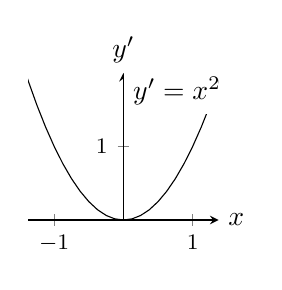
\begin{tikzpicture}
\begin{axis}[small,width=4cm,axis lines=middle,xlabel={$x$},ylabel={$y'$},xtick={-1,1},ytick={1},xlabel style={at={(current axis.right of origin)},anchor=west},ylabel style={at={(current axis.above origin)},anchor=south},ymax=2]
\addplot[domain=-1.5:1.5]{x^2};
\draw(axis cs:0,1.75)node[right,fill=white]{$y'=x^2$};
\end{axis}
\end{tikzpicture}
\end{subfigure}%
\caption{ترسیم برائے شکل \حوالہ{سوال_تفرق_درکار_پ}}
\label{شکل_سوال_تفرق_درکار_پ}
\end{figure}
\انتہا{سوال}
%======================
\ابتدا{سوال}\شناخت{سوال_تفرق_معلومات_تلاش_کریں_ب}
$y=\tfrac{x^4}{4}$
\انتہا{سوال}
%======================
\ابتدا{سوال}
کیا \عددی{y=x^3} کا کبھی منفی ڈھلوان ہو گا؟ اگر ہے تو کہاں ہو گا؟ اپنے جواب کی وجہ پیش کریں۔\\
جواب:\quad
\عددی{y'=3x^2} کبھی بھی منفی نہیں ہو گا۔
\انتہا{سوال}
%======================
\ابتدا{سوال}
کیا \عددی{y=2\sqrt{x}} کا افقی مماس پایا جاتا ہے؟ اگر پایا جاتا ہے تو کہاں پایا جاتا ہے۔ اپنے جواب کی وجہ پیش کریں۔
\انتہا{سوال}
%===========================
\ابتدا{سوال}
کیا قطع مکافی \عددی{y=2x^2-13x+5} کے مماس کا ڈھلوان \عددی{-1} ہو سکتا ہے۔اگر ممکن ہے تب اس مماس کی مساوات حاصل کریں اور وہ نقطہ تلاش کریں جہاں مماس منحنی کو مس کرتا ہے۔ اگر ممکن نہیں ہے تب اپنے جواب کی وجہ پیش کریں۔\\
جواب:\quad
ہاں، \عددی{y+16=-(x-3)} نقطہ \عددی{(3,-16)} پر مماس ہے۔
\انتہا{سوال}
%====================
\ابتدا{سوال}
کیا منحنی \عددی{y=\sqrt{x}} کا کوئی مماس \عددی{x} محور کو \عددی{x=-1} پر قطع کرتا ہے؟ ممکن ہونے کی صورت میں نقطہ مماس اور مماس کی مساوات تلاش کریں جبکہ غیر ممکن ہونے کی صورت میں وجہ پیش کریں۔ 
\انتہا{سوال}
%=======================
\ابتدا{سوال}
کیا \عددی{(-\infty,\infty)} پر قابل تفرق تفاعل کا تفرق \عددی{y=\lfloor x\rfloor} ہو سکتا ہے؟ اپنے جواب کی وجہ پیش کریں۔ \\
جواب:\quad
نہیں، چونکہ تفاعل \عددی{y=\lfloor x\rfloor} متوسط قیمت خاصیت پر پورا نہیں اترتا ہے۔
\انتہا{سوال}
%========================
\ابتدا{سوال}
\عددی{f(x)=\abs{x}} کے تفرق کو ترسیم کرنے کے بعد \عددی{y=\tfrac{\abs{x}-0}{x-0}=\tfrac{\abs{x}}{x}} ترسیم کریں۔ان سے آپ کیا نتیجہ اخذ کر سکتے ہیں؟
\انتہا{سوال}
%========================
\ابتدا{سوال}
یہ جانتے ہوئے کہ \عددی{x=x_0} پر تفاعل \عددی{f(x)} قابل تفرق ہے، آپ \عددی{x=x_0} پر تفاعل \عددی{-f} کی قابل تفرق ہونے کے بارے میں کیا کہہ سکتے ہیں؟ اپنے جواب کی وجہ پیش کریں۔\\
جواب:\quad
ہاں؛ 
$(-f)'(x)=-(f'(x))$
\انتہا{سوال}
%==================
\ابتدا{سوال}
کیا \عددی{t=7} پر \عددی{g(t)} کا قابل تفرق ہونے سے آپ \عددی{t=7} پر \عددی{3g} کے قابل تفرق ہونے کے بارے میں کچھ کہہ سکتے ہیں؟ اپنے جواب کی وجہ پیش کریں۔
\انتہا{سوال}
%======================
\ابتدا{سوال}
فرض کریں کہ \عددی{t} کی تمام قیمتوں کے لئے تفاعل \عددی{g(t)} اور \عددی{h(t)} معین ہیں اور \عددی{g(0)=h(0)=0} ہے۔ کیا \عددی{\lim_{t\to 0}\tfrac{g(t)}{h(t)}} موجود ہو گا؟ اگر حد موجود ہو تب کیا یہ حد ضرور صفر کے برابر ہو گا؟ اپنے جواب کی وجہ پیش کریں۔\\
جواب:\quad
\عددی{g(t)=mt} اور \عددی{h(t)=t} کے لئے \عددی{\lim_{t\to 0}\tfrac{g(t)}{h(t)}=m} ہو گا جو غیر صفر ہو سکتا ہے۔ 
\انتہا{سوال}
%======================
\ابتدا{سوال}
(ا) فرض کریں کہ \عددی{-1\le x\le 1} کے لئے تفاعل \عددی{f(x)} شرط \عددی{\abs{f(x)}\le x^2} کو مطمئن کرتا ہے۔ دکھائیں کہ \عددی{x=0} پر \عددی{f} قابل تفرق ہے اور \عددی{f'(0)} حاصل کریں۔ (ب) دکھائیں کہ \عددی{x=0} پر
\begin{align*}
f(x)=
\begin{cases}
x^2\sin \frac{1}{x},&x\ne 0\\
0,&x=0
\end{cases}
\end{align*}
قابل تفرق ہے اور \عددی{f'(0)} تلاش کریں۔


\انتہا{سوال}
%=========================
\موٹا{کمپیوٹر کا استعمال}

\ابتدا{سوال}
\عددی{0\le x\le 2} کے لئے \عددی{y=\tfrac{1}{2\sqrt{x}}} کو ترسیم کریں۔اس کے اوپر پہلے \عددی{h=1,0.5,0.1} لیتے ہوئے \عددی{y=\tfrac{\sqrt{x+h}-\sqrt{x}}{h}} ترسیم کریں اور بعد میں \عددی{h=-1,-0.5,-0.1} لے کر ترسیم کریں۔سمجھائیں کہ کیا ہو رہا ہے۔
\انتہا{سوال}
%=========================
\ابتدا{سوال}
\عددی{-2\le x\le 2} اور \عددی{0\le y\le 3} لیتے ہوئے \عددی{y=3x^2} ترسیم کریں۔اسی کے اوپر پہلے \عددی{h=2,1,0.2} لیتے ہوئے \عددی{y=\tfrac{(x+h)^3-x^3}{h}} ترسیم کریں اور بعد میں \عددی{h=-2,-1,-0.2} لے کر ترسیم کریں۔ سمجھائیں کیا ہو رہا ہے۔ 
\انتہا{سوال}
%=====================
\ابتدا{سوال}\ترچھا{وائشسٹراس کا نا قابل تفرق تفاعل}
وائشسٹراس تفاعل \عددی{f(x)=\sum_{n=0}^{\infty}()^n\cos(9^n\pi x)} کے پہلے آٹھ ارکان کا مجموعہ درج ذیل ہے۔
\begin{multline*}
g(x)=\cos (\pi x)+\big(\frac{2}{3}\big)^1\cos (9\pi x)+\big(\frac{2}{3}\big)^2\cos (9^2\pi x)\\
+\big(\frac{2}{3}\big)^3\cos (9^3\pi x)+\cdots+\big(\frac{2}{3}\big)^7\cos (9^7\pi x)
\end{multline*}
اس تفاعل کو ترسیم کریں۔ترسیم کی جسامت بڑی کرتے ہوئے دیکھیں کہ یہ کتنی بلدار ہے۔
\انتہا{سوال}
%=====================
سوال \حوالہ{سوال_تفرق_کمپیوٹر_سے_تلاش_الف} تا سوال \حوالہ{سوال_تفرق_کمپیوٹر_سے_تلاش_ب} میں کمپیوٹر استعمال کرتے ہوئے درج ذیل کریں۔
\begin{enumerate}[a.]

\item
\عددی{y=f(x)} ترسیم کرتے ہوئے اس کا رویہ دیکھیں۔
\item
عمومی جسامت قدم \عددی{h} لیتے ہوئے عمومی نقطہ \عددی{x}  پر حاصل تقسیم  \عددی{q} متعارف کریں۔
\item
\عددی{h\to 0} کرتے ہوئے حد لینے سے کون سا کلیہ حاصل ہوتا ہے؟
\item
\عددی{x=x_0} پر کرتے ہوئے تفاعل اور اس نقطے پر مماس ترسیم کریں۔
\item
\عددی{x_0} سے \عددی{x} کی بڑی اور چھوٹی قیمتیں جزو (ج) میں پر کریں۔ کیا کلیہ اور ترسیم ایک جیسا مطلب پیش کرتے ہیں؟
\item
جزو (ج) میں حاصل کیا گیا کلیہ ترسیم کریں۔اس کی قیمتیں منفی، مثبت یا صفر ہونے کا کیا مطلب ہے؟ کیا جزو (ا) کی ترسیم کے ساتھ اس کا کوئی مطلب بنتا ہے؟ اپنے جواب کی وجہ پیش کریں۔
\end{enumerate}

\ابتدا{سوال}\شناخت{سوال_تفرق_کمپیوٹر_سے_تلاش_الف}
$f(x)=x^3+x^2-x,\quad x_0=1$
\انتہا{سوال}
%=====================
\ابتدا{سوال}
$f(x)=x^{\tfrac{1}{3}}+x^{\tfrac{2}{3}},\quad x_0=1$
\انتہا{سوال}
%=====================
\ابتدا{سوال}
$f(x)=\tfrac{4x}{x^2+1},\quad x_0=2$
\انتہا{سوال}
%=====================
\ابتدا{سوال}
$f(x)=\tfrac{x-1}{3x^2+1},\quad x_0=-1$
\انتہا{سوال}
%=====================
\ابتدا{سوال}
$f(x)=\sin 2x,\quad x_0=\tfrac{\pi}{2}$
\انتہا{سوال}
%=====================
\ابتدا{سوال}\شناخت{سوال_تفرق_کمپیوٹر_سے_تلاش_ب}
$f(x)=x^2\cos x,\quad x_0=\tfrac{\pi}{4}$
\انتہا{سوال}
%=====================

\حصہ{قواعد تفرق}
اس حصے میں تفرق کی تعریف استعمال کیے بغیر تفاعل کا تفرق حاصل کرنا سکھایا جائے گا۔

\جزوحصہء{طاقت، مجموعے اور تفریق}
تفرق کا پہلا قاعدہ یہ ہے کہ مستقل کا تفرق صفر کے برابر ہے۔

\ابتدا{قاعدہ}\موٹا{مستقل کا تفرق}\فرہنگ{قاعدہ!تفرق مستقل}\فرہنگ{rule!differential of constant}\\
اگر \عددی{c} مستقل ہو تب \عددی{\tfrac{\dif}{\dif x} c=0} ہو گا۔
\انتہا{قاعدہ}
%=====================
\ابتدا{مثال}$\frac{\dif}{\dif x} (8)=0,\quad \frac{\dif}{\dif x}\big(-\frac{1}{2}\big)=0,\quad \frac{\dif}{\dif x}(\sqrt{3})=0$
\انتہا{مثال}
%=======================

\ابتدا{ثبوت قاعدہ}
ہم تفرق کی تعریف استعمال کرتے ہوئے \عددی{f(x)=c} کا تفرق حاصل کرتے ہیں (شکل \حوالہ{شکل_تفرق_مستقل_صفر_ہو_گا})۔ہر \عددی{x} پر درج ذیل ہو گا۔
\begin{align*}
f'(x)=\lim_{h\to 0}\frac{f(x+h)-f(x)}{h}=\lim_{h\to 0}\frac{c-c}{h}=\lim_{h\to 0}0=0
\end{align*} 
%
\begin{figure}
\centering
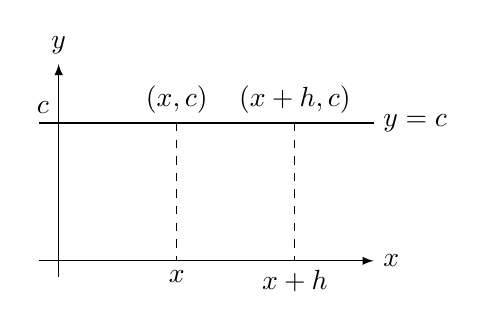
\begin{tikzpicture}
\draw[-latex](-0.25,0)--(4,0)node[right]{$x$};
\draw[-latex](0,-0.2)--(0,2.5)node[above]{$y$};
\draw(-0.25,1.75)--(4,1.75)node[right]{$y=c$};
\draw[dashed](1.5,1.75)node[above]{$(x,c)$}--(1.5,0)node[below]{$x$} (3,1.75)node[above]{$(x+h,c)$}--(3,0)node[below]{$x+h$};
\draw(0,1.75)node[above left]{$c$};
\end{tikzpicture}
\caption{مستقل کا تفرق صفر ہو گا۔}
\label{شکل_تفرق_مستقل_صفر_ہو_گا}
\end{figure}
\انتہا{ثبوت قاعدہ}

اگلا قاعدہ ہمیں \عددی{x^n} کا تفرق دیتا ہے جہاں \عددی{n} مثبت عدد صحیح ہے۔

\ابتدا{قاعدہ}\موٹا{قاعدہ طاقت برائے مثبت عدد صحیح}\فرہنگ{قاعدہ!طاقت}\فرہنگ{rule!power}\\
اگر \عددی{n} مثبت عدد صحیح ہو تب درج ذیل ہو گا۔
\begin{align*}
\frac{\dif}{\dif x} x^n=nx^{n-1}
\end{align*}
\انتہا{قاعدہ}
%=========================

قاعدہ طاقت استعمال کرتے ہوئے ہم  طاقت \عددی{n} سے \عددی{1} منفی کرتے ہوئے جواب کو \عددی{n} سے ضرب دیتے ہیں۔

\ابتدا{مثال}
\begin{align*}
\begin{array}{c|c|c|c|c|c}
f&x&x^2&x^3&x^4&\cdots\\
\hline
f'&1&2x&3x^2&4x^3&\cdots
\end{array}
\end{align*}
\انتہا{مثال}
%=======================
\ابتدا{ثبوت قاعدہ}
اگر \عددی{f(x)=x^n} ہو تب \عددی{f(x+h)=(x+h)^n} ہو گا۔چونکہ \عددی{n} مثبت عدد صحیح ہے ہم درج ذیل حقیقت 
\begin{align*}
a^n-b^n=(a-b)(a^{n-1+a^{n-2}b}+\cdots+ab^{n-2}+b^{n-1})
\end{align*}
استعمال کرتے ہوئے تفریقی حاصل تقسیم کی سادہ صورت حاصل کرتے ہیں۔ہم \عددی{a=x+h} اور \عددی{b=x} لیتے ہیں۔یوں \عددی{h=a-b} ہو گا۔اس طرح 
\begin{align*}
\frac{f(x+h)-f(x)}{h}&=\frac{(x+h)^n-x^n}{h}\\
&=\frac{(h)[(x+h)^{n-1}+(x+h)^{n-2}x+\cdots+(x+h)x^{n-2}+x^{n-1}]}{h}\\
&=(x+h)^{n-1}+(x+h)^{n-2}x+\cdots+(x+h)x^{n-2}+x^{n-1}
\end{align*}
لکھا جا سکتا ہے جو \عددی{n} ارکان پر مشتمل ہے اور  \عددی{h\to 0} کرتے ہوئے ہر رکن کا  حد \عددی{x^{n-1}} ہے۔یوں درج ذیل  نتیجہ حاصل ہوتا ہے۔ 
\begin{align*}
\frac{\dif}{\dif x}x^n=\lim_{h\to 0}\frac{f(x+h)-f(x)}{h}=nx^{n-1}
\end{align*}
\انتہا{ثبوت قاعدہ}
%=======================
اگلا قاعدہ کہتا ہے کہ قابل تفرق تفاعل کو مستقل سے ضرب دینے سے حاصل تفاعل کا تفرق بھی اس مستقل سے ضرب ہو گا۔

\ابتدا{قاعدہ}\شناخت{قاعدہ_تفرق_مضرب_مستقل}\موٹا{قاعدہ مستقل مضرب}\فرہنگ{قاعدہ!مستقل مضرب}\فرہنگ{rule!constant multiple}\\
اگر \عددی{u} متغیر \عددی{x} کا قابل تفرق تفاعل ہو اور \عددی{c} ایک مستقل ہو تب درج ذیل ہو گا۔
\begin{align*}
\frac{\dif}{\dif x} (cu)=c\frac{\dif u}{\dif x}
\end{align*}
\انتہا{قاعدہ}
%====================

بالخصوص مثبت عدد صحیح \عددی{n} کی صورت میں درج ذیل ہو گا۔
\begin{align*}
\frac{\dif}{\dif x} (cx^n)=cnx^{n-1}
\end{align*}

\ابتدا{مثال}\شناخت{مثال_تفرق_ڈھلوان_اور_مستقل}
تفرقی کلیہ \عددی{\tfrac{\dif}{\dif x}(3x^2)=3\cdot 2x=6x} کہتی ہے کہ \عددی{y} محور کو \عددی{3} سے ضرب دیتے ہوئے ترسیم \عددی{y=x^2} کی پیمائش تبدیل کرنے سے ہر نقطے کی ڈھلوان \عددی{3} سے ضرب ہو گی (شکل \حوالہ{شکل_مثال_تفرق_ڈھلوان_اور_مستقل})۔
\begin{figure}
\centering
\begin{tikzpicture}
\begin{axis}[clip=false,small,axis lines=middle,xlabel={$x$},ylabel={$y$},xtick={1,2},ytick={1,2,3}]
\addplot[domain=-0.25:2]{x^2}node[above,xshift={2mm}]{$y=x^2$};
\addplot[domain=-0.25:1.25]{3*x^2}node[left]{$y=3x^2$};
\draw[dashed](axis cs:1,0)--(axis cs:1,3)node[left]{$(1,3)$};
\draw[dashed](axis cs:1,1)node[circ]{}node[right]{$(1,1)$} (axis cs:1,3)node[circ]{};
\draw[shorten <=-1cm](axis cs:1,1)--(axis cs:1.5,2)node[right]{$m=2$};
\draw[shorten <=-1cm](axis cs:1,3)--(axis cs:1.2,4.2)node[right]{$m=6$};
\end{axis}
\end{tikzpicture}
\caption{ترسیم برائے مثال \حوالہ{مثال_تفرق_ڈھلوان_اور_مستقل}}
\label{شکل_مثال_تفرق_ڈھلوان_اور_مستقل}
\end{figure}
\انتہا{مثال}
%======================
\ابتدا{مثال}
قابل تفرق تفاعل کے منفی کا تفرق اس تفاعل کے تفرق کا منفی ہو گا۔قاعدہ \حوالہ{قاعدہ_تفرق_مضرب_مستقل} میں \عددی{c=-1} لیتے ہوئے درج ذیل ملتا ہے۔
\begin{align*}
\frac{\dif}{\dif x}(-u)=\frac{\dif}{\dif x}(-1\cdot u)=-1\cdot \frac{\dif}{\dif x}(u)=-\frac{\dif u}{\dif x}
\end{align*}
\انتہا{مثال}
%======================

\ابتدا{ثبوت قاعدہ} (قاعدہ \حوالہ{قاعدہ_تفرق_مضرب_مستقل})
\begin{align*}
\frac{\dif}{\dif x} cu&=\lim_{h\to 0}\frac{cu(x+h)-cu(x)}{h}&&\text{\RL{\عددی{f(x)=cu(x)} کے تفرق کی تعریف}}\\
&=c\lim_{h\to 0}\frac{u(x+h)-u(x)}{h} && \text{\RL{تحدیدی خاصیت}}\\
&=c\frac{\dif u}{\dif x}&&\text{\RL{\عددی{u} قابل تفرق ہے}}
\end{align*}
\انتہا{ثبوت قاعدہ}

اگلا قاعدہ کہتا ہے کہ دو قابل تفرق تفاعل کے مجموعے کا تفرق ان کے انفرادی تفرق کا مجموعہ ہو گا۔

\ابتدا{قاعدہ}\شناخت{قاعدہ_تفرق_مجموعہ}\موٹا{قاعدہ مجموعہ}\فرہنگ{قاعدہ!مجموعہ}\فرہنگ{rule!sum}\\
اگر \عددی{u} اور \عددی{v} متغیر \عددی{x} کے قابل تفرق تفاعل ہوں تب ان کا مجموعہ \عددی{u+v} ہر اس نقطے پر قابل تفرق ہو گا جہاں \عددی{u} اور \عددی{v} دونوں قابل تفرق ہوں۔ایسے نقطے پر درج ذیل ہو گا۔
\begin{align*}
\frac{\dif}{\dif x} (u+v)=\frac{\dif u}{\dif x}+\frac{\dif v}{\dif x}
\end{align*}
\انتہا{قاعدہ}
%================================

قاعدہ مجموعہ اور قاعدہ مستقل مضرب کو ملا کر مساوی \اصطلاح{تفریقی قاعدہ} حاصل ہو گا جس کے تحت دو قابل تفرق تفاعل کے حاصل تفریق کا تفرق ان کے تفرق کا تفریق ہو گا:
\begin{align*}
\frac{\dif}{\dif x} (u-v)=\frac{\dif}{\dif x}[u+(-1)v]=\frac{\dif u}{\dif x}+(-1)\frac{\dif v}{\dif x}=\frac{\dif u}{\dif x}-\frac{\dif v}{\dif x}
\end{align*} 

قاعدہ مجموعہ کو وسعت دے کر دو  سے زیادہ تفاعل کے لئے بھی استعمال کیا جا سکتا ہے بس اتنا ضروری ہے کہ مجموعہ میں ارکان کی تعداد متناہی ہو۔اگر \عددی{u_1,u_2,\cdots,u_n} متغیر \عددی{x} کے قابل تفرق تفاعل ہوں تب \عددی{u_1+u_2+\cdots+u_n} بھی قابل تفرق ہو گا اور اس کا تفرق درج ذیل ہو گا۔
\begin{align*}
\frac{\dif}{\dif x}(u_1+u_2+\cdots+u_n)=\frac{\dif u_1}{\dif x}+\frac{\dif u_2}{\dif x}+\cdots+\frac{\dif u_n}{\dif x}
\end{align*}

\ابتدا{مثال}
\begin{gather*}
\begin{aligned}[t]
\text{(ا)}\quad y&=x^4+12x\\
\frac{\dif y}{\dif x}&=\frac{\dif}{\dif x}(x^4)+\frac{\dif}{\dif x}(12x)\\
&=4x^3+12
\end{aligned}
\quad
\begin{aligned}[t]
\text{(ب)}\quad y&=x^3+\frac{4}{3}x^2-5x+1\\
\frac{\dif y}{\dif x}&=\frac{\dif}{\dif x}x^3+\frac{\dif}{\dif x}\big(\frac{4}{3}x^2\big)-\frac{\dif}{\dif x}(5x)+\frac{\dif}{\dif x}(1)\\
&=3x^2+\frac{4}{3}\cdot 2x-5+0\\
&=3x^2+\frac{8}{3}x-5
\end{aligned}
\end{gather*}
\انتہا{مثال}
%======================
آپ نے اس مثال میں دیکھا کہ کسی بھی کثیر رکنی کا جزو در جزو تفرق لیا جا سکتا ہے۔ 

\ابتدا{ثبوت قاعدہ} (قاعدہ \حوالہ{قاعدہ_تفرق_مجموعہ})
ہم تفرق کی تعریف کو \عددی{f(x)=u(x)+v(x)} پر لاگو کرتے ہیں۔
\begin{align*}
\frac{\dif}{\dif x}[u(x)+v(x)]&=\lim_{h\to 0}\frac{[u(x+h)+v(x+h)]-[u(x)+v(x)]}{h}\\
&=\lim_{h\to 0}\left[ \frac{u(x+h)-u(x)}{h}+\frac{v(x+h)-v(x)}{h}\right]\\
&=\lim_{h\to 0}\frac{u(x+h)-u(x)}{h}+\lim_{h\to 0}\frac{v(x+h)-v(x)}{h}\\
&=\frac{\dif u}{\dif x}+\frac{\dif v}{\dif x}
\end{align*}
\انتہا{ثبوت قاعدہ}
%==========================

\موٹا{دو سے زیادہ تفاعل کے مجموعہ کے لئے ثبوت}\\
ہم درج ذیل فقرے کو \اصطلاح{ریاضی ماخوذ}\حاشیہب{mathematical induction} کی مدد سے ثابت کرتے ہیں۔
\begin{align}\label{مساوات_تفرق_مجموعہ_الف}
\frac{\dif}{\dif x}(u_1+u_2+\cdots+u_n)=\frac{\dif u_1}{\dif x}+\frac{\dif u_2}{\dif x}+\cdots+\frac{\dif u_n}{\dif x}
\end{align}
جیسا اوپر ثابت کیا گیا درج بالا فقرہ \عددی{n=2} کے لئے درست ہے۔یہ ریاضی ماخوذ کا پہلا قدم ہے۔

دوسرے قدم میں ہم نے ثابت کرنا ہو گا کہ اگر یہ فقرہ کسی بھی مثبت عدد صحیح \عددی{n=k} (جہاں \عددی{k\ge n_0=2} ہے)  کے لئے درست ہے تب یہ \عددی{n=k+1} کے لئے بھی درست ہو گا۔ فرض کریں کہ
\begin{align*}
\frac{\dif}{\dif x}(u_1+u_2+\cdots+u_k)=\frac{\dif u_1}{\dif x}+\frac{\dif u_2}{\dif x}+\cdots+\frac{\dif u_k}{\dif x}
\end{align*}
ہے تب درج ذیل ہو گا۔
\begin{align*}
&\frac{\dif}{\dif x}(\underbrace{u_1+u_2+\cdots+u_k}_{\text{\RL{اس مجموعہ کو \عددی{u} کہیں}}}+\underbrace{u_{k+1}}_{\text{\RL{اس کو \عددی{v} کہیں}}})\\
&=\frac{\dif}{\dif x}(u_1+u_2+\cdots+u_k)+\frac{\dif u_{k+1}}{\dif x}\\
&=\frac{\dif u_1}{\dif x}+\frac{\dif u_2}{\dif x}+\cdots+\frac{\dif u_k}{\dif x}+\frac{\dif u_{k+1}}{\dif x}
\end{align*}
اس قدم کی تکمیل  ہر عدد صحیح \عددی{n\ge 2} کے لئے  قاعدہ \حوالہ{قاعدہ_تفرق_مجموعہ} کی درستگی کی تصدیق کرتا ہے۔

%=====================
\ابتدا{مثال}\شناخت{مثال_تفرق_ٹیڑی_منحنی}
کیا منحنی \عددی{y=x^4-2x^2+2} کا افقی مماس پایا جاتا ہے؟ اگر پایا جاتا ہے تب کہاں پایا جاتا ہے؟\\
حل:\quad افقی مماس وہاں ہو گا جہاں \عددی{\tfrac{\dif y}{\dif x}} صفر کے برابر ہو۔ان نقطوں کو حاصل کرنے کے لئے ہم \عددی{\tfrac{\dif y}{\dif x}} معلوم کرتے ہیں
\begin{align*}
\frac{\dif y}{\dif x}=\frac{\dif}{\dif x}(x^4-2x^2+2)=4x^3-4x
\end{align*}
اور اس کے بعد مساوات \عددی{\tfrac{\dif y}{\dif x}=0} کو \عددی{x} کے لئے حل کرتے ہیں۔
\begin{align*}
4x^3-4x&=0\\
4x(x^2-1)&=0\\
x&=0,1,-1
\end{align*}
منحنی \عددی{y=x^4-2x^2+2} کا افقی مماس \عددی{x=0,1,-1} پر پایا جاتا ہے جہاں منحنی کے مطابقتی نقطے \عددی{(-1,1)}، \عددی{(1,1)}، \عددی{(0,2)} ہیں (شکل \حوالہ{شکل_مثال_تفرق_ٹیڑی_منحنی})۔
\begin{figure}
\centering
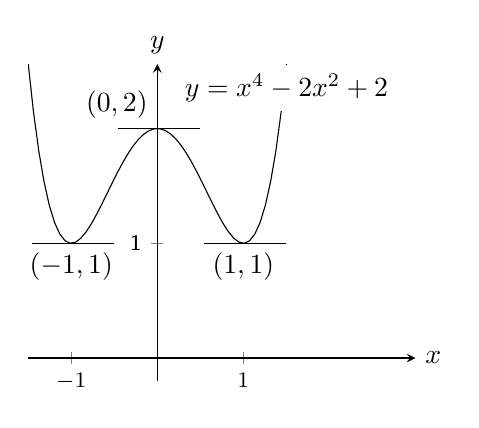
\begin{tikzpicture}
\begin{axis}[small,axis lines=middle,xlabel={$x$},ylabel={$y$},xtick={-1,1},ytick={1,1},ymin=-0.2,xmax=3,xlabel style={at={(current axis.right of origin)},anchor={west}},ylabel style={at={(current axis.above origin)},anchor=south}]
\addplot[domain=-1.5:1.5,samples=50]{x^4-2*x^2+2}node[below,fill=white]{$y=x^4-2x^2+2$};
\draw[shorten <=-0.5cm](axis cs:-1,1)--(axis cs:-0.5,1);
\draw[shorten <=-0.5cm](axis cs:1,1)--(axis cs:1.5,1);
\draw[shorten <=-0.5cm](axis cs:0,2)--(axis cs:0.5,2);
\draw(axis cs:-1,1)node[below]{$(-1,1)$} (axis cs:1,1)node[below]{$(1,1)$} (axis cs:0,2)node[above left]{$(0,2)$};
\end{axis}
\end{tikzpicture}
\caption{افقی مماس (مثال \حوالہ{مثال_تفرق_ٹیڑی_منحنی})}
\label{شکل_مثال_تفرق_ٹیڑی_منحنی}
\end{figure}
\انتہا{مثال}
%=====================
\جزوحصہء{حاصل ضرب اور حاصل تقسیم}
اگرچہ دو تفاعل کے مجموعہ کا تفرق ان تفاعل کے تفرق کا مجموعہ ہے، دو تفاعل کے حاصل ضرب کا تفرق ان تفاعل کے تفرق کا حاصل ضرب \ترچھا{نہیں} ہو گا۔مثال کے طور پر
\begin{align*}
\text{\RL{ہو گا۔}}\quad \frac{\dif}{\dif x}(x)\cdot \frac{\dif}{\dif x}(x)=1\cdot 1=1\quad\text{\RL{ہے جبکہ}}\quad \frac{\dif}{\dif x}(x\cdot x)=\frac{\dif}{\dif x}(x^2)=2x
\end{align*}
دو تفاعل کے حاصل ضرب کا تفرق دو حاصل ضرب کا مجموعہ ہو گا۔

\ابتدا{قاعدہ}\موٹا{قاعدہ حاصل ضرب}\فرہنگ{قاعدہ!حاصل ضرب}\فرہنگ{rule!product}\\
اگر \عددی{u} اور \عددی{v} متغیر \عددی{x} کے قابل تفرق تفاعل ہوں تب ان کا حاصل ضرب \عددی{uv} بھی \عددی{x} کا قابل تفرق تفاعل ہو گا جس کا تفرق درج ذیل ہو گا۔
\begin{align*}
\frac{\dif}{\dif x}(uv)=u\frac{\dif v}{\dif x}+v\frac{\dif u}{\dif x}
\end{align*}
\انتہا{قاعدہ}
%========================
حاصل ضرب \عددی{uv} کا تفرق \عددی{u} ضرب \عددی{v} کا تفرق جمع \عددی{v} ضرب \عددی{u} کا تفرق ہو گا۔اس کو \عددی{(uv)'=uv'+vu'} بھی لکھا جا سکتا ہے۔

\ابتدا{ثبوت قاعدہ}
تفرق کی تعریف کے تحت
\begin{align*}
\frac{\dif}{\dif x}(uv)=\lim_{h\to 0}\frac{u(x+h)v(x+h)-u(x)v(x)}{h}
\end{align*}
ہو گا جس کو \عددی{u} اور \عددی{v} کے تفریقی حاصل تقسیم کی صورت میں لکھنے کی خاطر ہم شمار کنندہ میں \عددی{u(x+h)v(x)} جمع اور منفی کرتے ہیں۔
\begin{align*}
\frac{\dif}{\dif x}(uv)&=\lim_{h\to 0}\frac{u(x+h)v(x+h)-u(x+h)v(x)+u(x+h)v(x)-u(x)v(x)}{h}\\
&=\lim_{h\to 0}\left[u(x+h)\frac{v(x+h)-v(x)}{h}+v(x)\frac{u(x+h)-u(x)}{h} \right]\\
&=\lim_{h\to 0} u(x+h)\cdot \lim_{h\to 0}\frac{v(x+h)-v(x)}{h}+v(x)\cdot\lim_{h\to 0}\frac{u(x+h)-u(x)}{h}
\end{align*}
چونکہ \عددی{x} پر \عددی{u} قابل تفرق ہے لہٰذا \عددی{h\to 0} کرنے سے \عددی{u(x+h)\to u(x)} ہو گا۔ دو کسر کی تحدیدی قیمتیں \عددی{x} پر  \عددی{\tfrac{\dif v}{\dif x}} اور \عددی{\tfrac{\dif u}{\dif x}} ہیں۔مختصراً درج ذیل ملتا ہے۔
\begin{align*}
\frac{\dif}{\dif x}(uv)=u\frac{\dif v}{\dif x}+v\frac{\dif u}{\dif x}
\end{align*}
\انتہا{ثبوت قاعدہ}
%============================
\موٹا{قاعدہ حاصل ضرب کی تصور کشی}\\
اگر \عددی{u(x)} اور \عددی{v(x)} مثبت ہوں اور \عددی{x} بڑھنے سے بڑھتے ہوں تب  \عددی{h>0} کی صورت میں شکل \حوالہ{شکل_تفرق_قاعدہ_ضرب_تصور_کشی} حاصل ہو گا۔\عددی{u(x)} اور \عددی{v(x)} بڑھنے سے رقبہ میں اضافہ
\begin{align*}
u(x+h)v(x+h)-u(x)v(x)=u(x+h)\Delta v+v(x+h)\Delta u-\Delta u\Delta v
\end{align*}
ہو گا جس کو ہلکا سیاہ رنگ دیا گیا ہے۔اس مساوات کے دونوں اطراف کو \عددی{h} سے تقسیم  کرنے سے
\begin{align*}
\frac{u(x+h)v(x+h)-u(x)v(x)}{h}&=u(x+h)\frac{\Delta v}{h}+v(x+h)\frac{\Delta u}{h}-\Delta u\frac{\Delta v}{h}
\end{align*}
حاصل ہو گا۔ اب \عددی{h\to 0^+}  کرنے سے \عددی{\Delta u\cdot \tfrac{\Delta v}{h}\to 0\cdot\tfrac{\dif v}{\dif x}=0} ہو گا لہٰذا درج ذیل باقی رہ جاتا ہے۔
\begin{align*}
\frac{\dif}{\dif x}(uv)=u\frac{\dif v}{\dif x}+v\frac{\dif u}{\dif x}
\end{align*} 
%
\begin{figure}
\centering
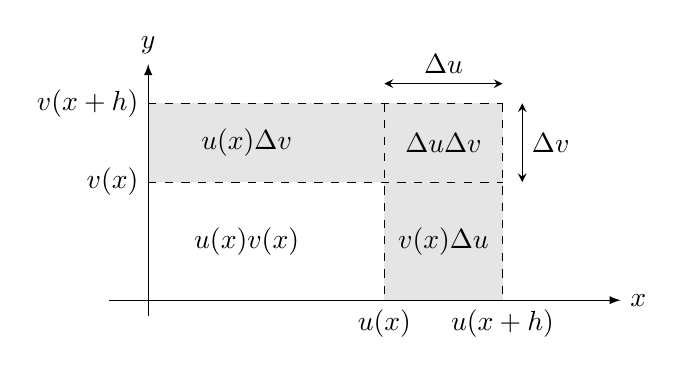
\begin{tikzpicture}
\fill[fill=gray!20](0,0) rectangle(4.5,2.5);
\fill[fill=white](0,0) rectangle(3,1.5);
\draw[-latex](-0.5,0)--(6,0)node[right]{$x$};
\draw[-latex](0,-0.2)--(0,3)node[above]{$y$};
\draw[dashed](0,2.5)node[left]{$v(x+h)$}--(4.5,2.5);
\draw[dashed](0,1.5)node[left]{$v(x)$}--(4.5,1.5);
\draw[dashed] (3,2.5)--(3,0)node[below]{$u(x)$};
\draw[dashed](4.5,2.5)--(4.5,0)node[below]{$u(x+h)$}; 
\draw(1.25,0.75)node[]{$u(x)v(x)$};
\draw(3.75,0.75)node[]{$v(x)\Delta u$};
\draw(1.25,2)node[]{$u(x)\Delta v$};
\draw(3.75,2)node[]{$\Delta u\Delta v$};
\draw[stealth-stealth] (3,2.75)--(4.5,2.75)node[pos=0.5,above]{$\Delta u$};
\draw[stealth-stealth] (4.75,2.5)--(4.75,1.5)node[pos=0.5,right]{$\Delta v$};
\end{tikzpicture}
\caption{قاعدہ حاصل ضرب کی تصور کشی۔}
\label{شکل_تفرق_قاعدہ_ضرب_تصور_کشی}
\end{figure}

%=======================
\ابتدا{مثال}\شناخت{مثال_تفرق_قاعدہ_حاصل_ضرب}
تفاعل \عددی{y=(x^2+1)(x^3+3)} کا تفرق تلاش کریں۔\\
حل:\quad
قاعدہ حاصل ضرب میں \عددی{u=x^2+1} اور \عددی{v=x^3+3} لیتے ہوئے درج ذیل ملتا ہے۔
\begin{align*}
\frac{\dif}{\dif x}[(x^2+1)(x^3+3)]&=(x^2+1)(3x^2)+(x^3+3)(2x)\\
&=3x^4+3x^2+2x^4+6x\\
&=5x^4+3x^2+6x
\end{align*}
\انتہا{مثال}
%=============================
 
اس مثال میں  قوسین کھول کر تفرق لینا غالباً زیادہ بہتر ہوتا۔ایسا کرنے سے
\begin{align*}
y&=(x^2+1)(x^3+3)=x^5+x^3+3x^2+3\\
\frac{\dif y}{\dif x}&=5x^4+3x^2+6x
\end{align*}
ملتا ہے جو مثال \حوالہ{مثال_تفرق_قاعدہ_حاصل_ضرب} میں حاصل جواب کی تصدیق کرتا ہے۔

بعض اوقات آپ دیکھیں گے کہ قاعدہ حاصل ضرب استعمال کرنا ضروری ہو گا یا نسبتاً زیادہ آسان ہو گا۔درج ذیل مثال میں ہمارے پاس صرف اعدادی قیمتیں ہیں جن سے ہمیں جواب حاصل کرنا ہے۔

\ابتدا{مثال}
فرض کریں کہ \عددی{y=uv} تفاعل \عددی{u} اور \عددی{v} کا حاصل ضرب ہے۔درج ذیل استعمال کرتے ہوئے \عددی{y'(2)} تلاش کریں۔
\begin{align*}
u(2)=3,\quad u'(2)=-4,\quad v(2)=1,\quad v'(2)=2
\end{align*}
حل:\quad
قاعدہ حاصل ضرب کی درج ذیل صورت
\begin{align*}
y'=(uv)'=uv'+vu'
\end{align*}
استعمال کرتے ہیں۔
\begin{align*}
y'(2)&=u(2)v'(2)+v(2)u'(2)\\
&=(3)(2)+(1)(-4)=6-4=2
\end{align*}
\انتہا{مثال}
%============================

\جزوحصہء{حاصل تقسیم}
جیسا تفاعل کے حاصل ضرب کا تفرق ان کے تفرق کا حاصل ضرب نہیں تھا اسی طرح تفاعل کے حاصل تقسیم کا تفرق ان کے تفرق کا حاصل تقسیم نہیں ہو گا۔درج ذیل قاعدہ اس کا حل دیتا ہے۔

\ابتدا{قاعدہ}\موٹا{قاعدہ حاصل تقسیم}\فرہنگ{قاعدہ!حاصل تقسیم}\فرہنگ{rule!quotient}\\
اگر \عددی{u(x)} اور \عددی{v()} متغیر \عددی{x} کے قابل تفرق تفاعل ہوں تب ان کا حاصل تقسیم \عددی{\tfrac{u}{v}} بھی \عددی{x} کا قابل تفرق تفاعل ہو گا اور یہ تفرق درج ذیل ہو گا۔
\begin{align*}
\frac{\dif}{\dif x}\big(\frac{u}{v}\big)=\frac{v\frac{\dif u}{\dif x}-u\frac{\dif v}{\dif x}}{v^2}
\end{align*}
\انتہا{قاعدہ}
%===========================
\ابتدا{ثبوت قاعدہ}
\begin{align*}
\frac{\dif}{\dif x}\big(\frac{u}{v}\big)&=\lim_{h\to 0}\frac{\frac{u(x+h)}{v(x+h)}-\frac{u(x)}{v(x)}}{h}\\
&=\lim_{h\to 0}\frac{v(x)u(x+h)-u(x)v(x+h)}{hv(x+h)v(x)}
\end{align*}
اس آخری کسر کو یوں تبدیل کرتے ہیں کہ اس میں \عددی{u} اور \عددی{v} کے تفریقی حاصل تقسیم پائے جاتے ہوں۔ایسا کرنے کی خاطر شمار کنندہ میں \عددی{v(x)u(x)} جمع اور منفی کرتے ہیں۔
\begin{align*}
\frac{\dif}{\dif x}\big(\frac{u}{v}\big)&=\lim_{h\to 0}\frac{v(x)u(x+h)-v(x)u(x)+v(x)u(x)-u(x)v(x+h)}{hv(x+h)v(x)}\\
&=\lim_{h\to 0}\frac{v(x)\frac{u(x+h)-u(x)}{h}-u(x)\frac{v(x+h)-v(x)}{h}}{v(x+h)v(x)}
\end{align*}
شمار کنندہ اور نسب نما میں حد لینے سے قاعدہ حاصل تقسیم حاصل ہوتا ہے۔
\انتہا{ثبوت قاعدہ}
%========================

\ابتدا{مثال}
تفاعل \عددی{y=\tfrac{t^2-1}{t^2+1}} کا تفرق تلاش کریں۔\\
حل:\quad
ہم \عددی{u=t^2-1} اور \عددی{v=t^2+1} لیتے ہوئے قاعدہ حاصل تقسیم استعمال کرتے ہیں۔
\begin{align*}
\frac{\dif y}{\dif t}&=\frac{(t^2+1)\cdot 2t-(t^2-1)\cdot 2t}{(t^2+1)^2}&&({\frac{\dif u}{\dif t}=2t,\,\, \frac{\dif v}{\dif t}=2t})\\
&=\frac{2t^3+2t-2t^3+2t}{(t^2+1)^2}\\
&=\frac{4t}{(t^2+1)^2}
\end{align*}
\انتہا{مثال}
%======================
\جزوحصہء{منفی عدد صحیح کے لئے طاقتی قاعدہ}
منفی عدد صحیح کا طاقتی قاعدہ اور مثبت عدد صحیح کا طاقتی قاعدہ ایک ہیں۔

\ابتدا{قاعدہ}\موٹا{منفی عدد صحیح کا طاقتی قاعدہ}\\
اگر \عددی{n} منفی عدد صحیح اور \عددی{x\ne 0} ہوں تب درج ذیل ہو گا۔
\begin{align*}
\frac{\dif}{\dif x}(x^n)=nx^{n-1}
\end{align*}
\انتہا{قاعدہ}
%========================
\ابتدا{ثبوت قاعدہ}
ہم قاعدہ حاصل تقسیم کو استعمال کر کے اس قاعدہ کو ثابت کرتے ہیں۔اگر \عددی{n} منفی عدد صحیح ہو تب \عددی{m=-n} مثبت عدد صحیح ہو گا۔یوں \عددی{x^n=x^{-m}=\tfrac{1}{x^m}} ہو گا لہٰذا درج ذیل لکھا جا سکتا ہے۔
\begin{align*}
\frac{\dif}{\dif x}(x^n)&=\frac{\dif}{\dif x}\big(\frac{1}{x^m}\big)\\
&=\frac{x^m\cdot \frac{\dif}{\dif x}(1)-1\cdot \frac{\dif}{\dif x}(x^m)}{(x^m)^2}&&\text{\RL{قاعدہ حاصل تقسیم جس میں \عددی{u=1} اور \عددی{v=x^m} ہیں}}\\
&=\frac{0-mx^{m-1}}{x^{2m}}&&\text{\RL{چونکہ \عددی{m>0} ہے لہٰذا \عددی{\tfrac{\dif}{\dif x}(x^m)=mx^{m-1}} ہو گا}}\\
&=-mx^{-m-1}\\
&=nx^{n-1}&&\text{\RL{چونکہ \عددی{-m=n} ہے}}
\end{align*}
\انتہا{ثبوت قاعدہ}
%========================

\ابتدا{مثال}
\begin{align*}
\frac{\dif}{\dif x}\big(\frac{1}{x}\big)&=\frac{\dif}{\dif x}(x^{-1})=(-1)x^{-2}=-\frac{1}{x^2}\\
\frac{\dif}{\dif x}\big(\frac{4}{x^3}\big)&=4\frac{\dif}{\dif x}(x^{-3})=4(-3)x^{-4}=-\frac{12}{x^4}
\end{align*}
\انتہا{مثال}
%======================
\ابتدا{مثال}
منحنی \عددی{y=x+\tfrac{2}{x}} کا نقطہ \عددی{(1,3)} پر مماس کی مساوات تلاش کریں۔\\
حل:\quad
منحنی کی ڈھلوان کی مساوات
\begin{align*}
\frac{\dif y}{\dif x}=\frac{\dif}{\dif x}(x)+2\frac{\dif}{\dif x}\big(\frac{1}{x}\big)=1+2\big(-\frac{1}{x^2}\big)=1-\frac{2}{x^2}
\end{align*}
ہے جس کی قیمت نقطہ \عددی{x=1} پر
\begin{align*}
\left.\frac{\dif y}{\dif x}\right\vert_{x=1}=\left[1-\frac{2}{x^2}\right]_{x=1}=1-2=-1
\end{align*}
ہو گی۔نقطہ \عددی{(1,3)} پر ڈھلوان \عددی{m=-1} کے خط کی مساوات حاصل کرتے ہیں۔
\begin{align*}
y-3&=(-1)(x-1)&&\text{\RL{نقطہ-ڈھلوان مساوات}}\\
y&=-x+1+3\\
y&=-x+4
\end{align*}
\انتہا{مثال}
%======================

\موٹا{قاعدہ کا انتخاب}\\
تفرق کے حصول میں موزوں قاعدے کا انتخاب حساب آسان بنا سکتا ہے۔درج ذیل مثال اس کی وضاحت کرتا ہے۔ 

\ابتدا{مثال}
قاعدہ حاصل تقسیم استعمال کرنے کی بجائے
\begin{align*}
y=\frac{(x-1)(x^2-2x)}{x^4}
\end{align*}
کے شمار کنندہ میں قوسین کھول کر \عددی{x^4} سے تقسیم کرتے ہیں
\begin{align*}
y=\frac{(x-1)(x^2-2x)}{x^4}=\frac{x^3-3x^2+2x}{x^4}=x^{-1}-3x^{-2}+2x^{-3}
\end{align*}
اور قاعدہ مجموعہ اور قاعدہ طاقت استعمال کرتے ہوئے تفرق حاصل کرتے ہیں۔
\begin{align*}
\frac{\dif y}{\dif x}&=-x^{-2}-3(-2)x^{-3}+2(-3)x^{-4}\\
&=-\frac{1}{x^2}+\frac{6}{x^3}-\frac{6}{x^4}
\end{align*}
\انتہا{مثال}
%=======================
\جزوحصہء{دو رتبی اور بلند رتبی تفرق}
تفرق \عددی{y'=\tfrac{\dif y}{\dif x}} کو \عددی{x} کے لحاظ سے \عددی{y} کا \اصطلاح{رتبہ اول تفرق}\فرہنگ{تفرق!رتبہ اول}\حاشیہب{first order derivative}\فرہنگ{derivative!first order} یا \اصطلاح{یک رتبی تفرق}\فرہنگ{تفرق!یک رتبی} یا مختصراً \اصطلاح{پہلا تفرق}\فرہنگ{تفرق!پہلا}\حاشیہب{first derivative}\فرہنگ{derivative!first} کہتے ہیں۔یہ تفرق ازخود \عددی{x} کے لحاظ سے قابل تفرق ہو سکتا ہے۔اگر ایسا ہو تب تفرق
\begin{align*}
y''=\frac{\dif y'}{\dif x}=\frac{\dif}{\dif x}\big(\frac{\dif y}{\dif x}\big)=\frac{\dif^{\,2} y}{\dif x^2}
\end{align*}
کو \عددی{x} کے لحاظ سے \عددی{y} کا \اصطلاح{رتبہ دوم تفرق}\فرہنگ{تفرق!رتبہ دوم}\حاشیہب{second order derivative}\فرہنگ{derivative!second order} یا \اصطلاح{دو رتبی تفرق}\فرہنگ{تفرق!دو رتبی} یا مختصراً \اصطلاح{دوسرا تفرق}\فرہنگ{تفرق!دوسرا}\حاشیہب{second derivative}\فرہنگ{derivative!second} کہتے ہیں۔

دو رتبی تفرق کی علامت  \عددی{\tfrac{\dif^{\,2}y}{\dif x^2}} میں شمار کنندہ میں \عددی{\dif} جبکہ نسب نما میں \عددی{x} کی طاقت \عددی{2} لکھی جاتی ہے۔درج بالا مساوات میں \عددی{\tfrac{\dif}{\dif x}\big(\tfrac{\dif y}{\dif x}\big)} سے مراد تفرقی علامتوں کا ضرب نہیں ہے بلکہ یہ تفرق کے تفرق کو ظاہر کرتی ہے۔

اگر \عددی{y''} قبل تفرق ہو تب اس کے تفرق \عددی{y'''=\tfrac{\dif y''}{\dif x}=\tfrac{\dif^{\,3}y}{\dif x^3}} کو \عددی{x} کے لحاظ سے \عددی{y} کا \اصطلاح{رتبہ سوم تفرق} یا \اصطلاح{سہ رتبی تفرق} یا \اصطلاح{تین رتبی تفرق}\فرہنگ{تفرق!تین رتبی} یا مختصراً \اصطلاح{تیسرا تفرق} کہتے ہیں۔اسی طرح بڑھتے ہوئے
\begin{align*}
y^{(n)}=\frac{\dif}{\dif x}y^{(n-1)}
\end{align*}
کو \عددی{x} کے لحاظ سے \عددی{y} کا \اصطلاح{رتبہ \عددی{n} تفرق} یا \اصطلاح{\عددی{n} رتبی تفرق}\فرہنگ{تفرق!این رتبی} یا \اصطلاح{\عددی{n} واں تفرق} کہیں گے جہاں \عددی{n} مثبت عدد صحیح ہے۔آپ نے دیکھا کہ بلند رتبی تفرق کو قوسین میں بند \عددی{y} کا طاقت لکھا جاتا ہے۔

\ابتدا{مثال}
تفاعل \عددی{y=x^3-3x^2+2} کے پہلے چار تفرق درج ذیل ہیں۔
\begin{align*}
y'&=3x^2-6x\\
y''&=6x-6\\
y'''&=6\\
y^{(4)}&=0
\end{align*}
چونکہ \عددی{y^{(4)}=0} ہے اور صفر ایک مستقل ہے لہٰذا اس کا تفرق در حقیقت صفر (یعنی مستال) کا تفرق ہو گا جو صفر ہی ہے۔یوں اس تفاعل کے ہر رتبے کا تفرق پایا جاتا ہے۔اس کا چار رتبی اور اس سے بلند تمام تفرق صفر کے برابر ہیں۔
\انتہا{مثال}
%======================

\حصہء{سوالات}
\موٹا{تفرق کا حساب}\\
سوال \حوالہ{سوال_تفرق_درجہ_اول_دوم_الف} تا سوال \حوالہ{سوال_تفرق_درجہ_اول_دوم_ب} میں تفاعل کا رتبہ اول اور رتبہ دوم تفرق حاصل کریں۔

\ابتدا{سوال}\شناخت{سوال_تفرق_درجہ_اول_دوم_الف}
$y=-x^2+3$\\
جواب:\quad
$y'=-2x,\quad y''=-2$
\انتہا{سوال}
%=======================
\ابتدا{سوال}
$y=x^2+x+8$
\انتہا{سوال}
%===========================
\ابتدا{سوال}
$s=5t^3-3t^5$\\
جواب:\quad
$s'=15t^2-15t^4,\quad s''=30t-60t^3$
\انتہا{سوال}
%===========================
\ابتدا{سوال}
$w=3z^7-7z^3+21z^2$
\انتہا{سوال}
%===========================
\ابتدا{سوال}
$y=\tfrac{4x^3}{3}-x$\\
جواب:\quad
$y'=4x^2-1,\quad y''=8x$
\انتہا{سوال}
%===========================
\ابتدا{سوال}
$y=\tfrac{x^3}{3}+\tfrac{x^2}{2}+\tfrac{x}{4}$
\انتہا{سوال}
%===========================
\ابتدا{سوال}
$w=3z^{-2}-\tfrac{1}{z}$\\
جواب:\quad
$w'=-6z^{-3}+\tfrac{1}{z^2},\quad w''=18z^{-4}-\tfrac{2}{z^3}$
\انتہا{سوال}
%===========================
\ابتدا{سوال}
$s=-2t^{-1}+\tfrac{4}{t^2}$
\انتہا{سوال}
%===========================
\ابتدا{سوال}
$y=6x^2-10x-5x^{-2}$\\
جواب:\quad
$y'=12x-10+10x^{-3},\quad y''=12-30x^{-4}$
\انتہا{سوال}
%===========================
\ابتدا{سوال}
$y=4-2x-x^{-3}$
\انتہا{سوال}
%===========================
\ابتدا{سوال}
$r=\tfrac{1}{3s^2}-\tfrac{5}{2s}$\\
جواب:\quad
$r'=-\tfrac{2}{3s^3}+\tfrac{5}{2s^2},\quad r''=\tfrac{2}{s^4}-\tfrac{5}{s^3}$
\انتہا{سوال}
%===========================
\ابتدا{سوال}\شناخت{سوال_تفرق_درجہ_اول_دوم_ب}
$r=\tfrac{12}{\theta}-\tfrac{4}{\theta^3}+\tfrac{1}{\theta^4}$
\انتہا{سوال}
%===========================

سوال \حوالہ{سوال_تفرق_قاعدہ_حاصل_تقسیم_الف} تا سوال \حوالہ{سوال_تفرق_قاعدہ_حاصل_تقسیم_ب} میں (ا) \عددی{y'} کو قاعدہ حاصل ضرب کی مدد سے حاصل کریں اور (ب) قوسین کو کھول کر سادہ ارکان حاصل کرتے ہوئے دوبارہ تفرق حاصل کریں۔

\ابتدا{سوال}\شناخت{سوال_تفرق_قاعدہ_حاصل_تقسیم_الف}
$y=(3-x^2)(x^3-x+1)$\\
جواب:\quad
$y'=-5x^4+12x^2-2x-3$
\انتہا{سوال}
%=======================
\ابتدا{سوال}
$y=(x-1)(x^2+x+1)$
\انتہا{سوال}
%=======================
\ابتدا{سوال}
$y=(x^2+1)\big(x+5+\tfrac{1}{x}\big)$\\
جواب:\quad
$y'=3x^2+10x+2-\tfrac{1}{x^2}$
\انتہا{سوال}
%=======================
\ابتدا{سوال}\شناخت{سوال_تفرق_قاعدہ_حاصل_تقسیم_ب}
$y=\big(x+\tfrac{1}{x}\big)\big(x-\tfrac{1}{x}+1\big)$
\انتہا{سوال}
%=======================
سوال \حوالہ{سوال_تفرق_تلاش_کریں_الف} تا سوال \حوالہ{سوال_تفرق_تلاش_کریں_ب} میں تفاعل کا تفرق تلاش کریں۔

\ابتدا{سوال}\شناخت{سوال_تفرق_تلاش_کریں_الف}
$y=\tfrac{2x+5}{3x-2}$\\
جواب:\quad
$y'=\tfrac{-19}{(3x-2)^2}$
\انتہا{سوال}
%======================
\ابتدا{سوال}
$z=\tfrac{2x+1}{x^2-1}$
\انتہا{سوال}
%======================
\ابتدا{سوال}
$g(x)=\tfrac{x^2-4}{x+0.5}$\\
جواب:\quad
$g'(x)=\tfrac{x^2+x+4}{(x+0.5)^2}$
\انتہا{سوال}
%======================
\ابتدا{سوال}
$f(t)=\tfrac{t^2-1}{t^2+t-2}$
\انتہا{سوال}
%======================
\ابتدا{سوال}
$v=(1-t)(1+t^2)^{-1}$\\
جواب:\quad
$\tfrac{\dif v}{\dif t}=\tfrac{t^2-2t-1}{(1+t^2)^2}$
\انتہا{سوال}
%======================
\ابتدا{سوال}
$w=(2x-7)^{-1}(x+5)$
\انتہا{سوال}
%======================
\ابتدا{سوال}
$f(s)=\tfrac{\sqrt{s}-1}{\sqrt{s}+1}$\\
جواب:\quad
$f'(s)=\tfrac{1}{\sqrt{s}(\sqrt{s}+1)^2}$
\انتہا{سوال}
%======================
\ابتدا{سوال}
$u=\tfrac{5x+1}{2\sqrt{x}}$
\انتہا{سوال}
%======================
\ابتدا{سوال}
$v=\tfrac{1+x-4\sqrt{x}}{x}$\\
جواب:\quad
$v'=-\tfrac{1}{x^2}+2x^{-3/2}$
\انتہا{سوال}
%======================
\ابتدا{سوال}
$r=2\big(\tfrac{1}{\sqrt{\theta}}+\sqrt{\theta}\big)$
\انتہا{سوال}
%======================
\ابتدا{سوال}
$y=\tfrac{1}{(x^2-1)(x^2+x+1)}$\\
جواب:\quad
$y'=\tfrac{-4x^3-3x^2+1}{(x^2-1)^2(x^2+x+1)^2}$
\انتہا{سوال}
%======================
\ابتدا{سوال}\شناخت{سوال_تفرق_تلاش_کریں_ب}
$y=\tfrac{(x+1)(x+2)}{(x-1)(x-2)}$
\انتہا{سوال}
%======================
\ابتدا{سوال}
تفاعل \عددی{y=\tfrac{x^4}{2}-\tfrac{3}{2}x^2-x} کے تمام بلند رتبی تفرق تلاش کریں۔\\
جواب:\quad
$y'=2x^3-3x-1, y''=6x^2-3,y'''=12x, y^{(4)}=12$
جبکہ تمام \عددی{n\ge 5} کے لئے 
$y^{(n)}=0$
\انتہا{سوال}
%========================
\ابتدا{سوال}
تفاعل \عددی{y=\tfrac{x^5}{120}} کے تمام بلند رتبی تفرق تلاش کریں۔
\انتہا{سوال}
%========================
سوال \حوالہ{سوال_تفرق_یک_درجی_دو_درجی_الف} تا سوال \حوالہ{سوال_تفرق_یک_درجی_دو_درجی_ب} میں یک رتبی اور دو رتبی تفرق تلاش کریں۔

\ابتدا{سوال}\شناخت{سوال_تفرق_یک_درجی_دو_درجی_الف}
$y=\tfrac{x^3+7}{x}$\\
جواب:\quad
$y'=2x-7x^{-2},\quad y''=2+14x^{-3}$
\انتہا{سوال}
%======================
\ابتدا{سوال}
$s=\tfrac{t^2+5t-1}{t^2}$
\انتہا{سوال}
%======================
\ابتدا{سوال}
$r=\tfrac{(\theta-1)(\theta^2+\theta+1)}{\theta^3}$\\
جواب:\quad
$\tfrac{\dif r}{\dif \theta}=3\theta^{-4},\quad \tfrac{\dif^{\,2}r}{\dif \theta^2}=-12\theta^{-5}$
\انتہا{سوال}
%======================
\ابتدا{سوال}
$u=\tfrac{(x^2+x)(x^2-x+1)}{x^4}$
\انتہا{سوال}
%======================
\ابتدا{سوال}
$w=\big(\tfrac{1+3z}{3z}\big)(3-z)$\\
جواب:\quad
$\tfrac{\dif w}{\dif z}=-z^{-2}-1,\quad \tfrac{\dif^{\,2}w}{\dif z^2}=2z^{-3}$
\انتہا{سوال}
%======================
\ابتدا{سوال}
$w=(z+1)(z-1)(z^2+1)$
\انتہا{سوال}
%======================
\ابتدا{سوال}
$p=\big(\tfrac{q^2+3}{12q}\big)\big(\tfrac{q^4-1}{q^3}\big)$\\
جواب:\quad
$\tfrac{\dif p}{\dif q}=\tfrac{1}{6}q+\tfrac{1}{6}q^{-3}+q^{-5},\quad \tfrac{\dif^{\,2}p}{\dif q^2}=\tfrac{1}{6}-\tfrac{1}{2}q^{-4}-5q^{-6}$
\انتہا{سوال}
%======================
\ابتدا{سوال}\شناخت{سوال_تفرق_یک_درجی_دو_درجی_ب}
$p=\tfrac{q^2+3}{(q-1)^3+(q+1)^3}$
\انتہا{سوال}
%======================
\موٹا{اعدادی قیمتوں کا استعمال}

\ابتدا{سوال}
فرض کریں کہ \عددی{u} اور \عددی{v} متغیر \عددی{x} کے تفاعل ہیں جو \عددی{x=0} پر قابل تفرق ہیں۔مزید ہمیں درج ذیل معلومات دی گئی ہے۔
\begin{align*}
u(0)=5,\quad u'(0)=-3,\quad v(0)=-1,\quad v'(0)=2
\end{align*}  
\عددی{x=0} پر درج ذیل تفرق تلاش کریں۔
\begin{align*}
\frac{\dif}{\dif x}(uv),\quad \frac{\dif}{\dif x}\big(\frac{u}{v}\big),\quad \frac{\dif}{\dif x}\big(\frac{v}{u}\big),\quad \frac{\dif}{\dif x}(7v-2u)
\end{align*}
جواب:\quad
\begin{align*}
\frac{\dif}{\dif x}(uv)=13,\,\frac{\dif}{\dif x}\big(\frac{u}{v}\big)=-7,\, \frac{\dif}{\dif x}\big(\frac{v}{u}\big)=\frac{7}{25},\, \frac{\dif}{\dif x}(7v-2u)=20
\end{align*}
\انتہا{سوال}
%=============================
\ابتدا{سوال}
فرض کریں کہ \عددی{u} اور \عددی{v} متغیر \عددی{x} کے قابل تفرق تفاعل ہیں۔مزید ہمیں درج ذیل معلومات دی گئی ہے۔
\begin{align*}
u(1)=2,\quad u'(1)=0,\quad v(1)=5,\quad v'(1)=-1
\end{align*}  
\عددی{x=1} پر درج ذیل تفرق تلاش کریں۔
\begin{align*}
\frac{\dif}{\dif x}(uv),\quad \frac{\dif}{\dif x}\big(\frac{u}{v}\big),\quad \frac{\dif}{\dif x}\big(\frac{v}{u}\big),\quad \frac{\dif}{\dif x}(7v-2u)
\end{align*}
\انتہا{سوال}
%=============================
\موٹا{ڈھلوان اور مماس}

\ابتدا{سوال}
(ا) نقطہ \عددی{(2,1)} پر منحنی \عددی{y=x^3-4x+1} کے مماس کے قائمہ کی مساوات تلاش کریں۔ (ب)   منحنی کی کم تر ڈھلوان  کتنی اور کس نقطے پر ہے؟ (ج) جس نقطے پر منحنی کے مماس کی ڈھلوان \عددی{8} ہے وہاں مماس کی مساوات تلاش کریں۔
\انتہا{سوال}
%=======================
\ابتدا{سوال}
(ا) منحنی \عددی{y=x^3-3x-2} کے افقی مماسوں کی مساواتیں تلاش کریں۔ مماسی نقطے پر مماس کے قائمہ کی مساواتیں بھی تلاش کریں۔ (ب) منحنی کی کم تر ڈھلوان کیا ہے اور کس نقطے پر ہے؟ اس نقطے پر مماس کے قائمہ کی مساوات تلاش کریں۔
\انتہا{سوال}
%========================
\ابتدا{سوال}
مبدا اور \عددی{(1,2)} پر منحنی \عددی{y=\tfrac{4x}{x^2+1}} کے مماسوں کی مساواتیں تلاش کریں۔ 
\انتہا{سوال}
%=====================
\ابتدا{سوال}
نقطہ \عددی{(2,1)} پر \عددی{y=\tfrac{8}{x^2+4}} کے مماس کی مساوات تلاش کریں۔
\انتہا{سوال}
%========================
\ابتدا{سوال}
منحنی \عددی{y=ax^2+bx+c} نقطہ \عددی{ً(1,2)} سے گزرتی ہے اور مبدا پر خط \عددی{y=x} کا مماس ہے۔\عددی{a}، \عددی{b} اور \عددی{c} تلاش کریں۔
\انتہا{سوال}
%======================
\ابتدا{سوال}
نقطہ \عددی{(1,0)} پر \عددی{y=x^2+ax+b} اور \عددی{y=cx-x^2} کا مشترک مماس پایا جاتا ہے۔\عددی{a}، \عددی{b} اور \عددی{c} تلاش کریں۔
\انتہا{سوال}
%=====================
\ابتدا{سوال}
(ا)  نقطہ \عددی{(-1,0)} پر منحنی \عددی{y=x^3-x} کے مماس کی مساوات تلاش کریں۔ (ب) کمپیوٹر پر منحنی اور مماس کو ترسیم کریں۔  مماس اس منحنی کو دوسرے نقطہ پر قطع کرتا ہے۔ ترسیم کو بڑا کرتے ہوئے اس نقطے کے  محدد کا اندازہ لگائیں۔ (ج) مماس اور منحنی کو اکٹھے حل کرتے ہوئے اس نقطے کی تصدیق کریں۔
\انتہا{سوال}
%========================
\ابتدا{سوال}
(ا) مبدا پر منحنی \عددی{y=x^3-6x^2+5x} کے مماس کی مساوات تلاش کریں۔ (ب) منحنی اور مماس کو کمپیوٹر پر ایک ساتھ ترسیم کریں۔ مماس اس منحنی کو دوسرے نقطے پر  قطع کرتا ہے۔ ترسیم کو بڑا کرتے ہوئے اس نقطے کے محدد کی اندازاً قیمت تلاش کریں۔ (ج) مماس اور منحنی کو اکٹھے حل کرتے ہوئے  اس نقطے کی تصدیق کریں۔
\انتہا{سوال}
%=========================
\موٹا{طبعی استعمال}

\ابتدا{سوال}\ترچھا{دباو اور حجم}\quad
بند ڈبہ میں مستقل درجہ حرارت \عددی{T} پر گیس کا حجم \عددی{V} اور دباو \عددی{P} درج ذیل کلیہ کو مطمئن کرتے ہیں جہاں \عددی{a}، \عددی{b} اور \عددی{c} مستقل ہیں۔ \عددی{\tfrac{\dif P}{\dif V}} تلاش کریں۔
\begin{align*}
P=\frac{nRT}{V-nb}-\frac{an^2}{V^2}
\end{align*}
\انتہا{سوال}
%====================
\ابتدا{سوال}\شناخت{سوال_تفرق_دوا_رد_عمل}\ترچھا{دوا کو جسم کا رد عمل}\quad
دوا کو جسم کے رد عمل  کو عموماً درج ذیل کلیہ  سے ظاہر کیا جا سکتا ہے جہاں \عددی{C} مثبت مستقل ہے جبکہ \عددی{M} خون میں جذب دوا کی مقدار ہے۔
\begin{align*}
R=M^2\big(\frac{C}{2}-\frac{M}{3}\big)
\end{align*}
اگر رد عمل فشار خون کی تبدیلی ہو تب \عددی{R} کو ملی میٹر پارہ میں ناپا جاتا ہے۔ اگر رد عمل درجہ حرارت میں تبدیلی ہو تب \عددی{R} کو کیلون میں ناپا جاتا ہے، وغیرہ وغیرہ۔ \عددی{\tfrac{\dif R}{\dif M}} تلاش کریں۔ یہ تفرق جو \عددی{M} کا تفاعل ہے،  دوا کی  مقدار میں تبدیلی کو جسم کی  \اصطلاح{حساسیت}\فرہنگ{حساسیت}\حاشیہب{sensitivity}\فرہنگ{sensitivity} کہلاتا ہے۔ سوال \حوالہ{سوال_استعمال_حساسیت} میں ہم دوا کی وہ مقدار معلوم کریں گے جس کو جسم  زیادہ سے زیادہ حساس ہو۔
\انتہا{سوال}
%========================
\موٹا{نظریہ اور مثالیں}

\ابتدا{سوال}
فرض کریں کہ قاعدہ حاصل ضرب میں \عددی{v} کی قیمت مستقل \عددی{c} ہو۔کیا اس سے قاعدہ مضرب مستقل حاصل کیا جا سکتا ہے؟
\انتہا{سوال}
%=========================
\ابتدا{سوال}\ترچھا{قاعدہ بالعکس متناسب}\\
(ا) \اصطلاح{قاعدہ بالعکس متناسب}\فرہنگ{قاعدہ!بالعکس متناسب}\حاشیہب{reciprocal rule}\فرہنگ{rule!reciprocal} کہتا ہے کہ جس نقطے پر تفاعل \عددی{v(x)} قابل تفرق ہو اس نقطے پر 
\begin{align*}
\frac{\dif}{\dif x}\big(\frac{1}{v}\big)=-\frac{1}{v^2}\frac{\dif v}{\dif x}
\end{align*}
ہو گا۔ دکھائیں کہ قاعدہ بالعکس متناسب در حقیقت قاعدہ حاصل تقسیم کی ایک مخصوص صورت ہے۔ (ب) دکھائیں کہ قاعدہ بالعکس متناسب اور قاعدہ حاصل ضرب کو ملا کر قاعدہ حاصل تقسیم  اخذ کیا جا سکتا ہے۔
\انتہا{سوال}
%====================
\ابتدا{سوال}\ترچھا{مثبت عدد صحیح کا دوسرا ثبوت}\quad
الجبرائی کلیہ
\begin{align*}
cx^n-c^n=(x-c)(x^{n-1}+x^{n-2}c+\cdots+xc^{n-2}+c^{n-1})
\end{align*}
اور صفحہ \حوالہ{مساوات_تفرق_متبادل_کلیہ} پر دیا گیا کلیہ تفرق (مساوات \حوالہ{مساوات_تفرق_متبادل_کلیہ})
\begin{align*}
f'(c)=\lim_{x\to c} \frac{f(x)-f(c)}{x-c}
\end{align*}
استعمال کرتے ہوئے \عددی{\tfrac{\dif}{\dif x}(x^n)=nx^{n-1}} حاصل کریں۔
\انتہا{سوال}
%====================
\ابتدا{سوال}\ترچھا{قاعدہ حاصل ضرب کی عمومی صورت}\quad
قاعدہ حاصل ضرب متغیر \عددی{x} کے قابل تفرق تفاعل \عددی{u} اور \عددی{v} کے لئے  درج ذیل کلیہ دیتا ہے۔
\begin{align*}
\frac{\dif}{\dif x}(uv)=u\frac{\dif v}{\dif x}+v\frac{\dif u}{\dif x}
\end{align*}
(ا) متغیر \عددی{x} کے قابل تفرق تین تفاعل کے حاصل ضرب \عددی{uvw} کے لئے کلیہ کیا ہو گا؟ (ب) متغیر \عددی{x} کے قابل تفرق چار تفاعل کے حاصل ضرب \عددی{u_1u_2u_3u_4} کے لئے کلیہ کیا ہو گا؟ (ج) متغیر \عددی{x} کے قابل تفرق متناہی تعداد  تفاعل کے حاصل ضرب \عددی{u_1u_2\cdots u_n} کے لئے کلیہ کیا ہو گا؟
\انتہا{سوال}
%==========================
\ابتدا{سوال}
\عددی{x^{3/2}} کو \عددی{x\cdot x^{1/2}} لکھ کر قاعدہ حاصل ضرب استعمال کرتے ہوئے \عددی{\tfrac{\dif}{\dif x}(x^{3/2})} حاصل کریں۔ جواب کو ناطق عدد ضرب \عددی{x} کا ناطق طاقت لکھیں۔ جزو (ب) اور (ج) کو بھی اسی طرح حل کریں۔ (ب) \عددی{\tfrac{\dif}{\dif x}(x^{5/2})} تلاش کریں۔ (ج) \عددی{\tfrac{\dif}{\dif x}(x^{7/2})} تلاش کریں۔ (د) درج بالا تین جزو میں آپ کیا نقش دیکھتے ہیں۔ ناطق طاقتیں حصہ \حوالہ{حصہ_خفی_تفرق_اور_ناطق_قوت_نما} کا ایک موضوع ہے۔
\انتہا{سوال}
%==========================

\حصہ{تبدیلی کی شرح}
اس حصے میں ہم تبدیلی کی شرح پر تفرق کی مدد  سے غور کریں گے۔ وقت کے لحاظ سے فاصلہ میں تبدیلی کی مثالیں سمتی رفتار اور اسراع ہیں۔ہم وقت کے علاوہ دیگر متغیر کے لحاظ سے بھی تبدیلی پر غور کر سکتے ہیں۔مثال کے طور پر حکیم  جاننا چاہے گا کہ دوا میں معمولی تبدیلی سے مریض کی حالت پر کیا اثر ہو گا۔ماہر اقتصادیات  جاننا چاہے گا کہ سرمایہ کاری میں معمولی تبدیلی سے اقتصادی ترقی پر کتنا اثر پایا جائے گا۔ان سوالات کو موزوں متغیر کے لحاظ سے تفرق کی صورت میں ظاہر کیا جائے گا۔

\جزوحصہء{اوسط اور لمحاتی شرح تبدیلی}
ہم کسی دورانیہ پر اوسط شرح تبدیلی سے شروع کرتے ہیں۔اس دورانیے کو صفر کے نزدیک تر کرنے سے حاصل شرح تبدیلی کی حد کو تفاعل کا تفرق کہتے ہیں۔

\ابتدا{تعریف}
\عددی{x} کے لحاظ سے وقفہ \عددی{x_0} تا \عددی{x_0+h} پر تفاعل \عددی{f(x)} کی \اصطلاح{اوسط شرح تبدیلی} سے مراد
\begin{align*}
\text{\RL{اوسط شرح تبدیلی}}=\frac{f(x_0+h)-f(x_0)}{h}
\end{align*}
ہے۔ \عددی{x} کے لحاظ سے \عددی{x_0} پر \عددی{f} کی \اصطلاح{(لمحاتی) شرح تبدیلی}
\begin{align*}
f'(x_0)=\lim_{x\to x_0}\frac{f(x_0+h)-f(x_0)}{h}
\end{align*}
کو کہتے ہیں بشرطیکہ یہ حد موجود ہو۔
\انتہا{تعریف}
%=========================

روایتی طور پر اگر \عددی{x} وقت کو ظاہر نہ کرتا ہو تب بھی لفظ \ترچھا{لمحاتی} استعمال کیا جاتا ہے۔عموماً \عددی{لمحاتی شرح تبدیلی} کو مختصراً \عددی{شرح تبدیلی} کہتے ہیں۔

\ابتدا{مثال}
دائرے کے رقبہ \عددی{S} اور رداس \عددی{r} کا تعلق درج ذیل ہے۔
\begin{align*}
S=\pi r^2
\end{align*}
رقبے کی شرح تبدیلی \عددی{r=\SI{0.1}{\meter}} پر کیا ہو گی؟\\
حل:\quad
رداس کے لحاظ سے رقبے کی (لمحاتی) شرح تبدیلی
\begin{align*}
\frac{\dif S}{\dif r}=2\pi r
\end{align*}
ہے۔یوں \عددی{r=\SI{0.1}{\meter}} کی صورت میں \عددی{r} تبدیل کرنے سے رقبہ تبدیل ہونے کی شرح \عددی{0.2\pi\, \si{\meter\squared/\meter}} ہو گی۔یوں  اس رداس پر رداس میں  \عددی{\Delta r} میٹر چھوٹی تبدیلی  سے رقبے میں  \عددی{0.2\pi\Delta r} مربع میٹر تبدیلی رونما ہو گی۔ 
\انتہا{مثال}
%========================

\جزوحصہء{لکیر پر حرکت۔ہٹاو، سمتی رفتار، رفتار اور اسراع}
فرض کریں کہ محوری خط (جس کو ہم \عددی{s} محور کہتے ہیں)  پر ایک جسم یوں حرکت کرتا ہے کہ اس محور پر مقام \عددی{s} اور وقت \عددی{t} کا تعلق 
\begin{align*}
s=f(t)
\end{align*}
ہے۔دورانیہ \عددی{t} تا \عددی{t+\Delta t} میں جسم کا \اصطلاح{ہٹاو}\فرہنگ{ہٹاو}\حاشیہب{displacement}\فرہنگ{displacement}
\begin{align*}
\Delta s=f(t+\Delta t)-f(t)
\end{align*}
ہو گا (شکل \حوالہ{شکل_تفرق_مقام_محور}) اور اس کی \اصطلاح{اوسط سمتی رفتار}\فرہنگ{سمتی رفتار!اوسط}\حاشیہب{average velocity}\فرہنگ{velocity!average}
\begin{align*}
v_{\text{اوسط}}=\frac{\text{ہٹاو}}{\text{دورانیہ}}=\frac{\Delta s}{\Delta t}=\frac{f(t+\Delta t)-f(t)}{\Delta t}
\end{align*}
ہو گی۔ ٹھیک لمحہ \عددی{t} پر جسم کی سمتی رفتار جاننے کی خاطر ہم \عددی{\Delta t \to 0} کرتے ہوئے دورانیہ \عددی{t} تا \عددی{t+\Delta t} پر اوسط سمتی رفتار کا حد تلاش کرتے ہیں۔یہ حد \عددی{t} کے لحاظ سے \عددی{f} کا تفرق ہے۔

\ابتدا{تعریف}
جسم کی (لمحاتی) سمتی رفتار وقت کے لحاظ سے تعین گر تفاعل \عددی{s=f(t)} کا تفرق ہو گا۔لمحہ \عددی{t} پر سمتی رفتار درج ذیل ہو گی۔
\begin{align*}
v(t)=\frac{\dif s}{\dif t}=\lim_{\Delta t\to 0}\frac{f(t+\Delta t)-f(t)}{\Delta t}
\end{align*} 
\انتہا{تعریف}
%====================

\ابتدا{مثال}\شناخت{مثال_تفرق_رفتار_گاڑھی}
 ایک گاڑھی کی  فاصلہ (میٹر) بالمقابل وقت (سیکنڈ) ترسیم کو شکل \حوالہ{شکل_مثال_تفرق_رفتار_گاڑھی} میں دکھایا گیا ہے۔سیکنٹ \عددی{NQ} کی ڈھلوان دورانیہ \عددی{t=\SI{5}{\second}} تا \عددی{\SI{15}{\second}} کے لئے اوسط سمتی رفتار ہے جو \عددی{\SI{32.5}{\meter\per\second}} یعنی \عددی{\SI{117}{\kilo\meter\per\hour}} کے برابر ہے۔لمحہ \عددی{t=\SI{5}{\second}} پر مماس کی ڈھلوان اس لمحہ پر لمحاتی سمتی رفتار \عددی{\SI{16.25}{\meter\per\second}} یعنی \عددی{\SI{58.5}{\kilo\meter\per\hour}} دیتی ہے۔
\begin{figure}
\centering
\begin{minipage}{0.45\textwidth}
\centering
\begin{tikzpicture}[font=\small]
\draw[-latex](0,0)--(4,0)node[right]{$s$}coordinate[pos=0.1](kL)node[pos=0.1,circ]{}node[pos=0.1,below]{$s=f(t)$}node[pos=0.7,circ]{}node[pos=0.7,below]{$s+\Delta s=f(t+\Delta t)$}coordinate[pos=0.7](kR);
\draw(kL)node[pin=90:{\RL{لمحہ $t$ پر مقام}}]{}   (kR)node[pin=90:{\RL{لمحہ $t+\Delta t$ پر مقام}}]{};
\end{tikzpicture}
\caption{محور پر حرکت کرتے جسم کا  \عددی{t} اور \عددی{t+\Delta t} پر مقام}
\label{شکل_تفرق_مقام_محور}
\end{minipage}\hfill
\begin{minipage}{0.45\textwidth}
\centering
\begin{tikzpicture}
\begin{axis}[grid=both,grid style={draw=gray},small,axis lines=middle,xlabel={$t$},ylabel={$s$},ymin=0,xlabel style={at={(current axis.right of origin)},anchor=west}]
\addplot[domain=0:22]{1/2*3.25*x^2};
\draw[](axis cs:5,40.625)node[circ]{}node[above left]{$N$}--(axis cs:15,365.625)node[circ]{}node[above left]{$Q$}node[pos=0.6,pin={[align=right]135:{\RL{سیکنٹ کی ڈھلوان}\\ \RL{اوسط سمتی رفتار ہے}}}]{};
\draw[shorten <=-0.5cm,shorten >=-0.5cm](axis cs:5,40.625)--(axis cs:10,121.875);
\draw(axis cs:12,180)node[right,align=right]{\RL{مماس کی ڈھلوان}\\  \RL{لمحاتی سمتی رفتار ہے}};
\end{axis}
\end{tikzpicture}
\caption{فاصلہ بالمقابل وقت برائے مثال \حوالہ{مثال_تفرق_رفتار_گاڑھی}}
\label{شکل_مثال_تفرق_رفتار_گاڑھی}
\end{minipage}%
\end{figure}
\انتہا{مثال}
%======================

\موٹا{مقدار معلوم روپ}\\
اگر \عددی{x} اور \عددی{y} دونوں متغیر \عددی{t} کے تفاعل ہوں تب \عددی{(x(t),y(t))} کی ترسیم \اصطلاح{مقدار معلوم ترسیم}\فرہنگ{مقدار معلوم!ترسیم}\حاشیہب{parametric curve}\فرہنگ{parametric!curve} کہلاتی ہے۔منحنی \عددی{y=f(x)} کی \اصطلاح{مقدار معلوم روپ}\فرہنگ{مقدار معلوم!روپ}\حاشیہب{parametric representation}\فرہنگ{parametric!representation} حاصل کرنے کی خاطر ہم \عددی{x=t} اور \عددی{y=f(t)} لیں گے۔چند منحنیات کی مقدار معلوم روپ درج ذیل ہے۔
\begin{align*}
\begin{array}{ll}
\multicolumn{1}{c}{\text{\RL{تفاعل}}}&\multicolumn{1}{c}{\text{\RL{مقدار معلوم روپ}}}\\
\hline
\Tstrut   y=x^2 (\text{\RL{$y$ متغیر $x$ کا تفاعل ہے}}) & x(t)=t,y(t)=t^2,-\infty<t<\infty\Bstrut\\
x^2+y^2=4 (\text{\RL{$y$ متغیر $x$ کا تفاعل نہیں ہے}}) & x(t)=2\cos t,y(t)=2\sin t,0\le t\le 2\pi
\end{array}
\end{align*} 


سمتی رفتار ہمیں فاصلہ طے کرنے کی شرح کے ساتھ ساتھ حرکت کی سمت بھی دیتی ہے۔ اگر جسم آگے (بڑھتے \عددی{s})  کی طرف  حرکت کرتا ہو تب سمتی رفتار مثبت ہو گا؛ اگر جسم پیچھے (گھٹے \عددی{s}) کی طرف حرکت کرتا ہو تب سمتی رفتار منفی ہو گا (شکل \حوالہ{شکل_تفرق_رفتار_مثبت_منفی})۔
\begin{figure}
\centering
\begin{subfigure}{0.5\textwidth}
\centering
\begin{tikzpicture}
\begin{axis}[small,axis lines=middle,xlabel={$t$},ylabel={$s$},xmin=0,ymin=0,xtick={\empty},ytick={\empty}]
\addplot[domain=0.5:2]{0.5+x^2}node[pos=0.8, above left]{$s=f(t)$}node[pos=0.5,below right]{$\frac{\dif s}{\dif t}>0$};
\end{axis}
\end{tikzpicture}
\caption{بڑھتا $s$ مثبت سمتی رفتار $v=\tfrac{\dif s}{\dif t}$ دیگا۔}
\end{subfigure}%
\begin{subfigure}{0.5\textwidth}
\centering
\begin{tikzpicture}
\begin{axis}[small,axis lines=middle,xlabel={$t$},ylabel={$s$},xmin=0,ymin=0,xtick={\empty},ytick={\empty}]
\addplot[domain=0.5:2]{5-x^2}node[pos=0.2, above right]{$s=f(t)$}node[pos=0.5,below left]{$\frac{\dif s}{\dif t}<0$};
\end{axis}
\end{tikzpicture}
\caption{گھٹتا $s$ منفی سمتی رفتار $v=\tfrac{\dif s}{\dif t}$ دیگا۔}
\end{subfigure}%
\caption{}
\label{شکل_تفرق_رفتار_مثبت_منفی}
\end{figure}
سمتی رفتار ایک جسم کتنا تیز فاصلہ طے کرتا ہے۔اس کے علاوہ ہمیں حرکت کرنے کی سمت کی معلومات بھی 

سمتی رفتار کی مطلق قیمت کو \اصطلاح{رفتار}\فرہنگ{رفتار}\حاشیہب{speed}\فرہنگ{speed} کہتے ہیں جو مثبت مقدار ہے۔ اگر آپ اپنے گھر سے  دوست  کے گھر تک \عددی{\SI{60}{\kilo\meter}} کی سمتی رفتار سے گاڑھی چلائیں اور وہاں سے واپسی پر اسی رفتار سے آئیں تو واپسی پر گاڑھی کی سمتی رفتار \عددی{\SI{-60}{\kilo\meter}} ہو گی لیکن گاڑھی کا رفتار پیما واپسی پر  بھی \عددی{\SI{60}{\kilo\meter\per\hour}} دکھائے گا چونکہ وہ رفتار ناپتا ہے نا کہ سمتی رفتار۔

\ابتدا{تعریف}
سمتی رفتار کی مطلق قیمت کو \اصطلاح{رفتار}\فرہنگ{رفتار}\حاشیہب{speed}\فرہنگ{speed} کہتے ہیں۔
\begin{align*}
\text{رفتار}=\abs{v(t)}=\abs{\frac{\dif s}{\dif t}}
\end{align*}
\انتہا{تعریف}
%==================

جس شرح سے ایک جسم کی سمتی رفتار تبدیل ہوتی ہے اس کو جسم کی \اصطلاح{اسراع} کہتے ہیں۔
%============================

\ابتدا{تعریف}
وقت کے لحاظ سے سمتی رفتار کا تفرق \اصطلاح{اسراع}\فرہنگ{اسراع}\حاشیہب{acceleration}\فرہنگ{acceleration} کہلاتا ہے۔اگر لمحہ \عددی{t} پر ایک جسم کا مقام \عددی{s=f(t)} ہو تب \عددی{t} پر اس جسم کی اسراع درج ذیل ہو گی۔
\begin{align*}
a(t)=\frac{\dif v}{\dif t}=\frac{\dif^{\,2}s}{\dif t^2}
\end{align*}
\انتہا{تعریف}
%==========================

ہوا کی مزاحمت کو نظر انداز کرتے ہوئے سطح زمین کے قریب ساکن حال سے گرتے ہوئے کسی بھی جسم سے اس کی وضاحت کی جا سکتی ہے۔ایسے جسم پر صرف کشش ثقل عمل کرتا ہے اور جسم کی حرکت کو \اصطلاح{آزادانہ گرنا}\فرہنگ{آزادانہ گرنا}\حاشیہب{free fall}\فرہنگ{free fall} کہتے ہیں۔آزادی سے گرتا ہوا جسم دورانیہ \عددی{t} میں 
\begin{align*}
s=\frac{1}{2}gt^2
\end{align*}
فاصلہ طے کرتا ہے جہاں مستقل \عددی{g=\SI{9.8}{\meter\per\second\squared}} سطح زمین کے قریب کشش زمین کی بنا اسراع ہے۔خلا میں ہوا کی غیر موجودگی کی بنا ہوا کی مزاحمت نہیں پائے جاتی ہے اور ہر جسم اس کے تحت حرکت کرتی ہے۔زمین کے قریب ہوا کی موجودگی میں ہر کثیف، بھاری جسم مثلاً اینٹ، پتھر، وغیرہ کی حرکت، ابتدائی چند سیکنڈ کے لئے جب تک ہوا کی مزاحمت قابل نظر انداز ہو، اس مساوات کو مطمئن کرتی ہے۔     

اسراع کی اکائی \عددی{\si{\meter\per\second\squared}}  میٹر فی مربع سیکنڈ پڑھی جاتی ہے۔

یہ مساوات ہمیں آزادانہ گرتے ہوئے جسم کی رفتار اور مقام کے بارے میں معلومات فراہم کرتی ہے۔

\ابتدا{مثال}
لمحہ \عددی{t=0} پر  ٹھوس جسم کو ساکن حال سے گرنے کے لئے چھوڑا جاتا ہے۔\\
(ا) پہلے \عددی{2} سیکنڈوں میں جسم کتنا فاصلہ طے کرتا ہے۔ (ب) اس لمحہ پر جسم کی رفتار اور اسراع کتنی ہوں گی؟\\
حل:\quad
(ا)\quad پہلے دو سیکنڈوں میں جسم درج ذیل فاصلہ طے کرتا ہے۔
\begin{align*}
s(2)=\frac{1}{2}(9.8)(2^2)=\SI{19.6}{\meter}
\end{align*}
(ب)\quad لمحہ \عددی{t} پر رفتار \عددی{v(t)} اور اسراع \عددی{a(t)} 
\begin{align*}
v(t)=\frac{\dif s}{\dif t}=9.8 t,\quad a=\frac{\dif v}{\dif t}=\frac{\dif^{\,2}s}{\dif t^2}=9.8
\end{align*}
ہوں گے۔یوں \عددی{t=\SI{2}{\second}} پر رفتار اور اسراع درج ذیل ہوں گے۔
\begin{align*}
v(2)=9.8(2)=\SI{19.6}{\meter},\quad a(2)=\SI{9.8}{\meter\per\second\squared}
\end{align*}
آپ نے دیکھا کہ اسراع \عددی{a} کی قیمت وقت \عددی{t} کا تابع نہیں ہے۔
\انتہا{مثال}
%==========================
\ابتدا{مثال}\شناخت{مثال_تفرق_آزاد_گرنا}
ایک جسم کو \عددی{\SI{49}{\meter\per\second}} کی ابتدائی رفتار کے ساتھ سیدھا اوپر پھینکا جاتا ہے۔ لمحہ \عددی{t} پر جسم  کی بلندی \عددی{s=49-\tfrac{1}{2}gt^2}  ہو گی (شکل \حوالہ{شکل_مثال_تفرق_آزاد_گرنا})۔\\
\begin{enumerate}[a.]

\item
جسم کس بلندی تک پہنچ پائے گا؟
\item
اوپر جاتے ہوئے \عددی{\SI{102.9}{\meter}} کی بلندی پر جسم کی سمتی رفتار کیا ہو گی؟ نیچے آتے ہوئے اتنی ہی بلندی پر سمتی رفتار کیا ہو گی؟
\item
حرکت کے دوران کسی بھی لمحہ \عددی{t} پر جسم کی اسراع کتنی ہو گی؟ 
\item
جسم زمین پر کب گرے گا؟
\end{enumerate}
حل:
\begin{enumerate}[a.]

\item
ہم محددی نظام یوں منتخب کرتے ہیں سطح زمین سے فاصلہ مثبت ہو۔یوں  بلندی \عددی{s} مثبت مقدار ہو گی،  ابتدائی رفتار مثبت ہو گی جبکہ اسراع جو نیچے رخ عمل کرتا ہے منفی ہو گا۔ اوپر جاتے ہوئے سمتی رفتار مثبت جبکہ نیچے گرتے ہوئے سمتی رفتار منفی ہو گی۔بلند ترین مقام پر سمتی رفتار صفر ہو گی۔ اب کسی بھی لمحہ پر سمتی رفتار
\begin{align*}
v(t)=\frac{\dif s}{\dif t}=49-gt
\end{align*}
ہو گی۔رفتار اس لمحہ پر صفر ہو گای جب 
\begin{align*}
49-9.8t=0,\quad \implies \quad t=\frac{49}{9.8}=\SI{5}{\second}
\end{align*} 
ہو۔لمحہ \عددی{t=\SI{5}{\second}} پر جسم کی بلندی درج ذیل ہو گی۔
\begin{align*}
s(5)=49(5)-\frac{1}{2}(9.8)(5^2)=\SI{122.5}{\meter}
\end{align*}
\item
جسم کی رفتار \عددی{\SI{100}{\meter}} پر حاصل کرنے کی خاطر ہم اس بلندی پر لمحہ \عددی{t} تلاش کرتے ہیں۔
\begin{align*}
102.9=49t-4.9t^2,\quad \implies \quad t=\SI{3}{\second},\,\SI{7}{\second}
\end{align*}
یوں \عددی{3} سیکنڈوں میں جسم \عددی{\SI{102.9}{\meter}} بلندی تک پہنچتا ہے جبکہ واپس گرتے ہوئے اسی بلندی پر یہ \عددی{7} سیکنڈ بعد ہوتا ہے۔ان لمحات پر جسم کی سمتی رفتار حاصل کرتے ہیں۔
\begin{align*}
v(3)=49-9.8(3)=\SI{19.6}{\meter\per\second},\quad v(7)=49-9.8(7)=\SI{-19.6}{\meter\per\second}
\end{align*}
آپ نے دیکھا کہ دونوں لمحات پر جسم کی رفتار ایک جیسی ہے۔
\item
جسم کی اسراع تلاش کرتے ہیں۔
\begin{align*}
a(t)=\frac{\dif^{\,2}s}{\dif t^2}=-g=\SI{-9.8}{\meter\per\second\squared}
\end{align*}
جسم کی اسراع مسلسل \عددی{\SI{-9.8}{\meter\per\second\squared}} رہتی ہے۔اوپر جاتے ہوئے یہ سمتی رفتار کو گھٹاتی ہے جبکہ نیچے گرتے کے دوران یہ سمتی رفتار میں اضافہ پیدا کرتا ہے۔ 
\item
جس اس لمحہ زمین پر ہو گا جب \عددی{s=0} ہو یعنی:
\begin{align*}
49t-4.9t^2=0,\quad \implies \quad t(49-4.9t)=0,\quad \implies \quad t=\SI{0}{\second}, \, \SI{10}{\second}
\end{align*}
یوں ابتدائی لمحے پر جسم زمین پر ہو گا اور ٹھیک \عددی{10} سیکنڈ بعد یہ واپس زمین پر گرتا ہے۔آپ دیکھ سکتے ہیں کہ اوپر جانے کا دورانیہ اور نیچے گرنے کا دورانیہ ایک جیسے ہیں۔
\end{enumerate}
%
\begin{figure}
\centering
\begin{tikzpicture}
\begin{axis}[clip=false,small,axis lines=middle,xlabel={$t$},ylabel={$s,v$},xtick={5,10},ytick={-49,49,122.5},xmax=12,ymin=-55,ymax=135,ylabel style={at={(current axis.above origin)},anchor=south}]
\addplot[domain=0:10]{49*x-4.9*x^2}node[pos=0.75,fill=white]{$s=49t-4.9t^2$};
\addplot[domain=0:10]{49-9.8*x}node[pos=1,below left]{$v=\frac{\dif s}{\dif t}=49-9.8t$};
\end{axis}
\end{tikzpicture}
\caption{بلندی اور سمتی رفتار (برائے مثال \حوالہ{مثال_تفرق_آزاد_گرنا})}
\label{شکل_مثال_تفرق_آزاد_گرنا}
\end{figure}
\انتہا{مثال}
%=============================

\موٹا{فنیات} \quad \ترچھا{انتصابی لکیر پر حرکت کی نقل} \\
مقدار معلوم مساوات
\begin{align*}
x(t)=c,\quad y(t)=f(t)
\end{align*}
کو کمپیوٹر پر  \اصطلاح{نقطہ ترسیم}\فرہنگ{ترسیم!نقطہ}\حاشیہب{dot graph}\فرہنگ{graph!dot} کریں جو لمحہ \عددی{t} پر نقطہ \عددی{(x(t),y(t))} دکھائے گی۔نقطہ ترسیم لمحہ با لمحہ صورت حال دکھاتی ہے۔یوں اگر \عددی{f(t)} جسم کی بلندی کو ظاہر کرتا ہو تب \عددی{(x(t),y(t))=(c,f(t))} کی لمحاتی ترسیم جسم کی حقیقی حرکت دکھائے گی۔مثال \حوالہ{مثال_تفرق_آزاد_گرنا} کے لئے اس لمحاتی ترسیم کو پہلے \عددی{0\le t\le 5} اور بعد میں \عددی{0\le t\le 10} وقفے پر دیکھیں۔

دوسرا تجربہ کرنے کی خاطر مقدار معلوم مساوات
\begin{align*}
x(t)=t,\quad y(t)=49t-4.9t^2
\end{align*}
کو نقطہ ترسیم کریں۔

\جزوحصہء{حساسیت}
اگر \عددی{x} میں چھوٹی تبدیلی سے  تفاعل \عددی{f(x)} میں بڑی تبدیلی رونما ہوتی ہو تب ہم کہتے ہیں کہ  \عددی{x} میں تبدیلی کے لئے  تفاعل نسبتاً زیادہ \اصطلاح{حساس}\فرہنگ{حساس}\حاشیہب{sensitive}\فرہنگ{sensitive} ہے۔تفرق \عددی{f'(x)} تفاعل \عددی{f(x)} کی \اصطلاح{حساسیت}\فرہنگ{حساسیت}\حاشیہب{sensitivity}\فرہنگ{sensitivity} کی ناپ ہے۔

\ابتدا{مثال}\quad \ترچھا{تبدیلی کے لئے حساسیت}\\
آسٹریا کے گرگر یوہان مینڈل (1822-1884) نے مٹر پر تجربہ کرتے ہوئے  \اصطلاح{جنیات}\فرہنگ{جنیات}\حاشیہب{genetics}\فرہنگ{genetics} کے میدان کی بنیاد ڈالی۔ ان کے نتائج کے مطابق اگر ہموار جلد والے (\اصطلاح{غالب}\فرہنگ{غالب}\حاشیہب{dominant}\فرہنگ{dominant}) مٹروں   کے \اصطلاح{جین}\فرہنگ{جین}\حاشیہب{gene}\فرہنگ{gene} کی تعدد \عددی{p} ہو (جہاں \عددی{p} کی قیمت \عددی{0} تا \عددی{1} ہو سکتی ہے) اور غیر  ہموار جلد والے (\اصطلاح{مغلوب}\فرہنگ{مغلوب}\حاشیہب{recessive}\فرہنگ{recessive}) مٹروں کی جین کی تعدد \عددی{(1-p)} ہو تب مٹروں کی  آبادی میں ہموار جلد مٹروں کی تناسب
\begin{align*}
y=2p(1-p)+p^2=2p-p^2
\end{align*}
ہے۔

\عددی{y} بالمقابل \عددی{p} کی ترسیم کے مطابق جب \عددی{p} کی قیمت کم ہو تب \عددی{y} زیادہ حساس ہو گا (شکل \حوالہ{شکل_تفرق_مینڈل_تجربہ}-ا)۔ تفاعل \عددی{y} کے تفرق  \عددی{\tfrac{\dif y}{\dif p}} کی ترسیم سے بھی یہی ظاہر ہوتا ہے۔جب \عددی{p} کی قیمت \عددی{0} کے قریب ہو تب \عددی{\tfrac{\dif y}{\dif p}} کی قیمت \عددی{2} کے قریب ہے اور جب \عددی{p} کی قیمت \عددی{1} کے قریب ہو تب \عددی{\tfrac{\dif y}{\dif p}} کی  قیمت \عددی{0} کے قریب ہے (شکل \حوالہ{شکل_تفرق_مینڈل_تجربہ}-ب)۔  
\begin{figure}
\centering
\begin{subfigure}{0.5\textwidth}
\centering
\begin{tikzpicture}
\begin{axis}[small,axis lines=middle,xlabel={$p$},ylabel={$y$},xtick=1,ytick=1,xmax=2,ymax=1.5,xlabel style={at={(current axis.right of origin)},anchor=west},ylabel style={at={(current axis.above origin)},anchor=south}]
\addplot[domain=0:1]{2*x-x^2}node[pos=0.5,right]{$y=2p-p^2$};
\end{axis}
\end{tikzpicture}
\caption{ہموار جلد مٹروں کی تناسب \عددی{y=2p-p^2}}
\end{subfigure}%
\begin{subfigure}{0.5\textwidth}
\centering
\begin{tikzpicture}
\begin{axis}[small,axis lines=middle,xlabel={$p$},ylabel={$\tfrac{\dif y}{\dif p}$},xtick=1,ytick=2,xmax=2,ymax=3,xlabel style={at={(current axis.right of origin)},anchor=west},ylabel style={at={(current axis.above origin)},anchor=south}]
\addplot[domain=0:1]{2-2*x}node[pos=0.5,above right]{$\frac{\dif y}{\dif p}=2-2p$};
\end{axis}
\end{tikzpicture}
\caption{حساسیت}
\end{subfigure}
\caption{مینڈل کے تجربہ نے جنیات کی بنیاد  رکھی۔}
\label{شکل_تفرق_مینڈل_تجربہ}
\end{figure}
\انتہا{مثال}
جیسے تفرق کی بات کرتے ہوئے سمتی رفتار اور اسراع کی اصطلاحات استعمال کی جاتی ہیں،   اقتصادیات کی میدان میں ہم \اصطلاح{حاشیہ}\فرہنگ{حاشیہ }\حاشیہب{marginals}\فرہنگ{marginals} کی بات کرتے ہیں۔ 

عمل پیداوار میں اشیاء پیدا کرنے کی لاگت \عددی{c(x)} متغیر \عددی{x} کا تفاعل ہے جہاں پیدا کردہ اشیاء کی تعداد  \عددی{x} ہے۔ \اصطلاح{حاشیہ لاگت پیداوار}\فرہنگ{حاشیہ لاگت پیداوار}\حاشیہب{marginal cost of production}\فرہنگ{marginal!cost of production} سے مراد پیدا وار کے لحاظ سے لاگت کی شرح تبدیلی \عددی{\tfrac{\dif c}{\dif x}} ہے۔ 

مثال کے طور پر ایک ہفتہ میں \عددی{x} ٹن\حاشیہب{tonne, \SI{1000}{\kilo\gram}} فولاد پیدا کرنے پر \عددی{c(x)} روپیہ  لاگت آتی ہے۔اب \عددی{x+h} ٹن فولاد پیدا کرنے پر زیادہ لاگت آئے گی اور لاگت میں اضافہ (تبدیلی) کو \عددی{h} سے تقسیم کرنے سے فی ہفتہ فی ٹن لاگت میں اوسط اضافہ ہو گا۔
\begin{align*}
\frac{c(x+h)-c(x)}{h}=\text{\RL{ہفتہ میں \عددی{h} ٹن اضافی فولاد پیدا کرنے سے لاگت میں اوسط اضافہ}}
\end{align*} 
فی ہفتہ موجودہ پیداوار \عددی{x} ٹن ہونے کی صورت میں \عددی{h\to 0} کرتے ہوئے اس نسبت کا حد اضافی فولاد پیدا کرنے کی \ترچھا{حاشیہ لاگت}\فرہنگ{حاشیہ لاگت} دے گی (شکل \حوالہ{شکل_تفرق_حاشیہ_لاگت_پیداوار}-ا)۔
\begin{align*}
\frac{\dif c}{\dif x}=\lim_{h\to 0}\frac{c(x+h)-c(x)}{h}=\text{\RL{حاشیہ لاگت پیداوار}}
\end{align*}
بعض اوقات ہم اضافی ایک اکائی پیداوار کی اضافی لاگت
\begin{align*}
\frac{\Delta c}{\Delta x}=\frac{c(x+1)-c(x)}{1}
\end{align*}
 کو ہی حاشیہ لاگت پیداوار کہتے ہیں جو \عددی{x} پر \عددی{\tfrac{\dif c}{\dif x}} کی تخمین ہے۔یہ قابل قبول اس لئے ہے کہ \عددی{x} کے نزدیک \عددی{c} کی ڈھلوان میں تبدیلی زیادہ نہیں ہوتی ہے لہٰذا یہاں \عددی{\Delta x=1} لیتے ہوئے حاصل سیکنٹ کی ڈھلوان کی قیمت حد \عددی{\tfrac{\dif c}{\dif x}} کے  قیمت کے بہت قریب ہو گی۔ عملاً \عددی{x} کی بڑی قیمتوں کے لئے یہ تخمین قابل قبول ہو گی (شکل \حوالہ{شکل_تفرق_حاشیہ_لاگت_پیداوار}-ب)۔
\begin{figure}
\centering
\begin{subfigure}{0.5\textwidth}
\centering
\begin{tikzpicture}
\draw[-latex](-0.5,0)--(3.5,0)node[right]{$x\,$\RL{(ٹن فی ہفتہ)}};
\draw[-latex](0,-0.2)--(0,2)node[above]{$y\,$\RL{(روپیہ)}};
\draw(0.5,0.5) to [out=45,in=-160]coordinate[pos=0.4](kA)coordinate[pos=0.405](kB)coordinate[pos=0.8](kC) (3,2)node[above]{$y=c(x)$};
\draw[shorten <=-1cm, shorten >=-1cm](kA)--(kB)node[rotate=30,above]{\RL{ڈھلوان$\,=\,$حاشیہ لاگت}};
\draw[dashed](kA)node[circ]{}--($(0,0)!(kA)!(3.5,0)$)node[below]{$x$};
\draw[dashed](kC)node[circ]{}--($(0,0)!(kC)!(3.5,0)$)node[below]{$x+h$};
\end{tikzpicture}
\caption{ہفتہ وار پیداوار بالمقابل لاگت}
\end{subfigure}%
\begin{subfigure}{0.5\textwidth}
\centering
\begin{tikzpicture}[font=\small]
\draw[-latex](-0.5,0)--(3.5,0)node[right]{$x$};
\draw[-latex](0,-0.2)--(0,2)node[above]{$y$};
\draw(0.5,0.5) to [out=45,in=-160]coordinate[pos=0.4](kA)coordinate[pos=0.405](kB)coordinate[pos=0.8](kC) (3,2)node[above right]{$y=c(x)$};
\draw[name path=kTan,shorten <=-1cm](kA)--++(35:1.5);
\path[name path=kR](kC)node[circ]{}--++(0,0.5);
\path[name path=kR,name intersections={of=kR and kTan}] (intersection-1)coordinate(kT)--($(0,0)!(intersection-1)!(3.5,0)$);
\draw[dashed](kA)node[circ]{}--($(0,0)!(kA)!(3.5,0)$)node[below]{$x$};
\path[name path=kBot](kA)--++(1.5,0);
\draw[name intersections={of=kBot and kR}] (intersection-1)--(kT)node[circ]{} (intersection-1)--(kA)node[pos=0.5,below,font=\tiny]{$\Delta x=1$};
\draw[dashed] (intersection-1)--($(0,0)!(intersection-1)!(3.5,0)$)node[below]{$x+1$};
\draw[name path=kLL](intersection-1)++(0.1,0)--++(1,0);
\draw(kC)++(0.1,0)--++(0.2,0)coordinate[pos=0.5](kDT);
\path[name path=kDropL](kDT)--++(0,-1.5);
\draw[stealth-stealth,name intersections={of=kDropL and kLL}] (kDT)--(intersection-1)node[pos=0.5,right]{$\Delta c$};
\draw(kT)++(0.1,0)--++(1,0)coordinate[pos=0.75](kTR);
\path[name path=kDropR](kTR)--++(0,-1.5);
\draw[stealth-stealth,name intersections={of=kDropR and kLL}] (kTR)--(intersection-1)node[pos=0.5,right]{$\tfrac{\dif c}{\dif x}$};
\end{tikzpicture}
\caption{\عددی{\Delta x=1} اضافی پیداوار کی اضافی لاگت \عددی{\Delta c} تقریباً \عددی{\tfrac{\dif c}{\dif x}} کے برابر ہے۔}
\end{subfigure}%
\caption{حاشیہ لاگت پیداوار}
\label{شکل_تفرق_حاشیہ_لاگت_پیداوار}
\end{figure}

\ابتدا{مثال}\ترچھا{حاشیہ لاگت}
فرض کریں کہ  \عددی{x} اشیاء پیدا کرنے  پر
\begin{align*}
c(x)=x^3-6x^2+15x
\end{align*}
روپیہ لاگت آتی ہے جب \عددی{x} کی قیمت \عددی{8} تا \عددی{30} ہو۔ ابھی آپ روزانہ \عددی{10} اشیاء پیدا کرتے ہیں۔روزانہ ایک اضافی شہ پیدا کرنے پر کتنی 
 اضافی لاگت آئے گی؟\\
حل:\quad
دس اشیاء بناتے ہوئے مزید ایک شہ پیدا کرنے پر تقریباً \عددی{c'(10)} اضافی لاگت آئے گی
\begin{align*}
c'(x)&=\frac{\dif}{\dif x}(x^3-6x^2+15x)=3x^2-12x+15\\
c'(10)&=3(100)-12(10)+15=195
\end{align*}
جو \عددی{195} روپیہ کے برابر ہے۔
\انتہا{مثال}
%=============================

اگرچہ حقیقی اعمال کے کلیات عموماً نہیں پائے جاتے ہیں، نظریہ اقتصادیات ہمیں متوقع نتائج جاننے میں مدد کرتا ہے۔یہ نظریہ جن تفاعل کا ذکر کرتا ہے انہیں عموماً موزوں وقفہ پر کم درجے کی کثیر رکنیوں سے ظاہر کرنا ممکن ہوتا ہے۔ کعبی کثیر رکنی عموماً اس قابل ہوتی ہے کہ پیچیدہ مسئلے کو ظاہر کر سکے اور کعبی کثیر رکنی  کا  استعمال  زیادہ مشکل بھی نہیں ہوتا ہے۔ 

\ابتدا{مثال}\ترچھا{حاشیہ شرح ٹیکس}\\
اگر آپ نی موجودہ آمدن پر حاشیہ شرح ٹیکس \عددی{\SI{28}{\percent}} ہو اور آپ کی آمدنی میں \عددی{10000} روپیہ کا اضافہ ہو تب آپ کو اضافی \عددی{2800} روپیہ ٹیکس ادا کرنا ہو گا۔  \عددی{\SI{28}{\percent}} حاشیہ ٹیکس کا یہ ہرگز مطلب نہیں ہے کہ آپ کو اپنی آمدن کا \عددی{\SI{28}{\percent}} بطور ٹیکس ادا کرنا ہو گا۔ اس کا مطلب صرف یہ ہے کہ آپ کی موجودہ آمدنی \عددی{I} پر آمدنی بڑھنے کے لحاظ سے ٹیکس کی شرح \عددی{\tfrac{\dif T}{\dif I}=0.28} ہے۔ آپ کو ہر اضافی ایک روپیہ کی آمدن پر \عددی{0.28} روپیہ ٹیکس ادا کرنا ہو گا۔ اب ظاہر ہے کہ اگر آپ کی آمدن بہت بڑھ جائے تب آپ ٹیکس کے نئے قالب میں شامل ہوں جائیں گے جہاں حاشیہ شرح ٹیکس غالباً زیادہ ہو گا۔  
\انتہا{مثال}
%=======================
\ابتدا{مثال}\ترچھا{حاشیہ}
اگر \عددی{x} ہزار مٹھائی فروخت کرنے سے 
\begin{align*}
r(x)=x^3-3x^2+12x
\end{align*}
آمدنی حاصل ہو جہاں \عددی{5\le x\le 20} ہے تب \عددی{10} ہزار مٹھائی فروخت کرتے ہوئے حاشیہ آمدنی
\begin{align*}
r'(x)=\frac{\dif}{\dif x}(x^3-3x^2+12x)=3x^2-6x+12
\end{align*}
ہو گی۔حاشیہ لاگت کی طرح ایک اضافی اکائی فروخت کرنے سے آمدنی میں اضافہ کو حاشیہ آمدنی پیش کرتی ہے۔اگر آپ \عددی{10} ہزار مٹھائیاں فی ہفتہ فروخت کر رہے ہوں تب فی ہفتہ \عددی{11} ہزار مٹھائیاں فروخت کرنے سے آپ کی آمدنی میں درج ذیل روپیہ اضافہ متوقع ہو گا۔
\begin{align*}
r'(10)=3(100)-6(10)+12=252
\end{align*} 
\انتہا{مثال}
%=====================

\حصہء{سوالات}
\موٹا{محددی لکیر پر حرکت}\\
سوال \حوالہ{سوال_تفرق_محددی_لکیر_الف} تا سوال \حوالہ{سوال_تفرق_محددی_لکیر_ب} میں \عددی{a\le t\le b} کے لئے \عددی{s=f(t)} محددی لکیر پر ایک جسم کا مقام دیتی ہے جہاں \عددی{t} کی اکائی سیکنڈ اور \عددی{s} کی اکائی میٹر ہے۔
\begin{enumerate}[a.]

\item
دیے گئے وقفے پر جسم کا ہٹاو اور سمتی رفتار حاصل کریں۔
\item
اس وقفے کے  آخری سروں پر جسم کی رفتار اور اسراع تلاش کریں۔
\item
جسم کب حرکت کی سمت تبدیل کرتا ہے (اگر ایسا کرتا ہو)؟   
\end{enumerate}

\ابتدا{سوال}\شناخت{سوال_تفرق_محددی_لکیر_الف}
$s=0.8t^2,\quad 0\le t\le 10 \quad \text{\RL{چاند پر آزادانہ گرنا}}$\\
جواب:\quad(ا) \عددی{\SI{80}{\meter}}، \عددی{\SI{8}{\meter\per\second}} (ب) \عددی{\SI{0}{\meter\per\second}}، \عددی{\SI{16}{\meter\per\second}}؛ \عددی{\SI{1.6}{\meter\per\second\squared}}، \عددی{\SI{1.6}{\meter\per\second\squared}} (ج) سمت  تبدیلی نہیں ہوتی
\انتہا{سوال}
%======================
\ابتدا{سوال}
$s=1.86t^2,\quad 0\le t\le 0.5\quad \text{\RL{مریخ پر آزادانہ گرنا}}$
\انتہا{سوال}
%========================
\ابتدا{سوال}
$s=-t^3+3t^2-3t,\quad 0\le t\le 3$\\
جواب:\quad
(ا) \عددی{\SI{-9}{\meter}}، \عددی{\SI{-3}{\meter\per\second}} (ب) \عددی{\SI{3}{\meter\per\second}}، \عددی{\SI{12}{\meter\per\second}}؛ \عددی{\SI{6}{\meter\per\second\squared}}، \عددی{\SI{-12}{\meter\per\second\squared}} (ج) سمت  تبدیلی  نہیں ہوتی
\انتہا{سوال}
%=========================
\ابتدا{سوال}
$s=\tfrac{t^4}{4}-t^3+t^2,\quad 0\le t\le 2$
\انتہا{سوال}
%=========================
\ابتدا{سوال}
$s=\tfrac{25}{t^2}-\tfrac{5}{t},\quad 1\le t\le 5$\\
جواب:\quad
(ا) \عددی{\SI{-20}{\meter}}، \عددی{\SI{-5}{\meter\per\second}} (ب) \عددی{\SI{45}{\meter\per\second}}،
 \عددی{\SI{0.2}{\meter\per\second}}؛ \عددی{\SI{140}{\meter\per\second\squared}}، \عددی{\tfrac{4}{25}\,\si{\meter\per\second\squared}} (ج) سمت تبدیل نہیں ہوتی
\انتہا{سوال}
%========================
\ابتدا{سوال}\شناخت{سوال_تفرق_محددی_لکیر_ب}
$s=\tfrac{25}{t+5},\quad -4\le t\le 0$
\انتہا{سوال}
%========================
\ابتدا{سوال}
\عددی{s} محور پر لمحہ \عددی{t} پر  ایک جسم کا مقام \عددی{s=t^3-6t^2+9t} ہے۔ (ا) ان نقطوں پر اس جسم کی اسراع تلاش کریں جن پر جسم کی سمتی رفتار صفر ہو گی۔ (ب) جب جسم کی اسراع صفر ہو اس لمحے پر اس جسم کی رفتار کیا ہو گی؟ (ج) لمحہ \عددی{t=0} تا \عددی{t=2} کے دوران یہ جسم کل کتنا فاصلہ طے کرتی ہے۔\\
جواب:\quad (ا) \عددی{a(1)=\SI{-6}{\meter\per\second\squared}}، \عددی{a(3)=\SI{6}{\meter\per\second\squared}} (ب) \عددی{v(2)=\SI{3}{\meter\per\second}} (ج) \عددی{\SI{6}{\meter}}
\انتہا{سوال}
%==========================
\ابتدا{سوال}
وقت \عددی{t\ge 0} پر \عددی{s} محور پر حرکت کرتے ہوئے جسم کی سمتی رفتار \عددی{v=t^2-4t+3} ہے۔ (ا) جسم کی اسراع وہاں تلاش کریں جہاں جسم کی سمتی رفتار صفر ہے۔ (ب)  جسم کب آگے رخ اور کب پیچھے رخ حرکت کرتی ہے؟ (ج) جسم کی سمتی رفتار کب بڑھتی اور کب گھٹتی ہے؟
\انتہا{سوال}
%============================
\موٹا{آزادانہ گرنا}

\ابتدا{سوال}
مریخ اور مشتری کی سطح کے قریب آزادانہ گرنے کے مساوات بالترتیب \عددی{s=1.86t^2} اور \عددی{s=11.44t^2} ہیں جہاں \عددی{t} کی اکائی سیکنڈ اور \عددی{s} کی اکائی میٹر ہے۔ ساکن حال سے گرتے ہوئے کتنے وقت میں (مریخ اور مشتری میں) ایک جسم کی رفتار \عددی{\SI{27.8}{\meter\per\second}} یعنی تقریباً \عددی{\SI{100}{\kilo\meter\per\hour}} ہو گی؟\\
جواب:\quad مریخ: \عددی{\SI{7.5}{\second}}، مشتری: \عددی{\SI{1.2}{\second}}
\انتہا{سوال}
%========================
\ابتدا{سوال}\شناخت{سوال_تفرق_پتھر_مریخ}
سطح چاند سے  انتصابی رخ \عددی{\SI{25}{\meter\per\second}} کی رفتار سے  پھینکا گیا پتھر \عددی{t} سیکنڈوں میں \عددی{s=24t-0.8t^2} میٹر بلندی پر پہنچے گا۔
\begin{enumerate}[a.]

\item
لمحہ \عددی{t} پر پتھر کی اسراع کیا ہو گی؟ (یہ اسراع چاند پر کشش ثقل کی اسراع ہو گی۔)
\item
پتھر بلند ترین مقام تک کتنے دورانیے میں پہنچے گا؟
\item
پتھر کتنی بلندی تک پہنچ پائے گا؟
\item
بلند ترین مقام کی نصف تک پتھر کتنی دیر میں پہنچے گا؟
\item
پتھر  کتنے وقت میں سطح چاند پر گرے گا؟ 
\end{enumerate}   
\انتہا{سوال}
%=========================
\ابتدا{سوال}
سطح زمین پر ہوا کی  غیر موجودگی میں سوال \حوالہ{سوال_تفرق_پتھر_مریخ} کا پتھر \عددی{t} سیکنڈوں میں \عددی{s=24t-4.9t^2} بلندی پر ہو گا۔
\begin{enumerate}[a.]

\item
لمحہ \عددی{t} پر پتھر کی اسراع کیا ہو گی؟ (یہ اسراع چاند پر کشش ثقل کی اسراع ہو گی۔)
\item
پتھر بلند ترین مقام تک کتنے دورانیے میں پہنچے گا؟
\item
پتھر کتنی بلندی تک پہنچ پائے گا؟
\item
بلند ترین مقام کی نصف تک پتھر کتنی دیر میں پہنچے گا؟
\item
پتھر  کتنے وقت میں سطح چاند پر گرے گا؟ 
\end{enumerate}   
جواب:\quad
(ا) \عددی{2.4-9.8t\,\si{\meter\per\second}}، \عددی{\SI{-9.8}{\meter\per\second\squared}} (ب) \عددی{\SI{2.4}{\second}} (ج) \عددی{\SI{29.4}{\meter}} (د) \عددی{0.7} سیکنڈ اوپر جانب اور \عددی{4.2} سیکنڈ نیچے رخ (ہ) \عددی{\SI{4.9}{\second}} 
\انتہا{سوال}
%========================
\ابتدا{سوال}
ہوا سے خالی ایک دنیا پر ایک ٹھوس جسم کو انتصابی رخ \عددی{\SI{15}{\meter\per\second}} کی ابتدائی رفتار سے پھینکا گیا۔ اس دنیا کے سطح پر ثقلی اسراع  \عددی{g_s \,\si{\meter\per\second\squared}} ہونے کی بنا \عددی{t} سیکنڈوں میں جسم \عددی{s=15t-\tfrac{1}{2}g_st^2}  میٹر بلندی تک پہنچے گا۔یہ جسم بلند ترین مقام تک \عددی{20} سیکنڈوں میں پہنچتا ہے۔ اس دنیا میں ثقلی اسراع کتنی ہے؟
\انتہا{سوال}
%==========================
\ابتدا{سوال}
چاند پر ایک بندوق کو انتصابی رخ چلایا گیا۔بندوق کی گولی \عددی{t} سیکنڈوں میں \عددی{s=300t-4.9t^2} میٹر بلندی پر ہو گی۔چاند پر یہی گولی \عددی{t} سیکنڈ بعد \عددی{s=300t-0.8t^2} میٹر بلندی پر ہو گی۔دونوں صورتوں میں گولی کتنی دیر بعد سطح پر گرے گی؟\\
جواب:\quad
چاند پر \عددی{320} سیکنڈ، زمین پر \عددی{52} سیکنڈ؛  چاند پر \عددی{20287} میٹر، زمین پر \عددی{3297} میٹر
\انتہا{سوال}
%=============================
\ابتدا{سوال}
مشتری پر ہوا کی غیر موجودگی میں یہی گولی \عددی{t} سیکنڈ بعد \عددی{s=300t-11.44t^2} میٹر بلندی پر ہو گی جبکہ مریخ پر یہ \عددی{s=300t-1.86t^2} میٹر کی بلندی پر ہو گی۔دونوں صورتوں میں گولی کتنے بلندی تک پہنچے گی؟
\انتہا{سوال}
%=================
\ابتدا{سوال}\شناخت{سوال_تفرق_تجربہ_گلیلو}\ترچھا{گلیلو کا کلیہ برائے آزادانہ گرنا}
ایک پٹی کو مختلف زاویوں پر رکھتے ہوئے گلیلو نے اس پر گیند کی سمتی رفتار کو ناپتے ہوئے کلیہ اخذ کیا جس کی تحدیدی صورت سے آزادانہ گرتے ہوئے جسم کی سمتی رفتار کا کلیہ حاصل کرنا مقصد تھا (شکل \حوالہ{شکل_سوال_تفرق_تجربہ_گلیلو})۔گلیلو نے دیکھا کہ حرکت کے شروع سے \عددی{t} سیکنڈ بعد سمتی رفتار کی قیمت \عددی{t} کے راست متناسب ہے یعنی  \عددی{v=kt} لکھا جا سکتا ہے۔ مستقل \عددی{k} کی قیمت کا دارومدار پٹی کی ڈھلوان پر ہے۔
\begin{figure}
\centering
\begin{subfigure}[b]{0.45\textwidth}
\centering
\begin{tikzpicture}
\draw(-2,0)--(4,0);
\draw[thick](0,0)--++(160:2)coordinate[pos=0.8](kA);
\draw(kA)++(160-90:0.25)circle(0.25);
\draw[thick](1,0)--++(140:2)coordinate[pos=0.8](kA);
\draw(kA)++(140-90:0.25)circle(0.25);
\draw[thick](2,0)--++(120:2)coordinate[pos=0.8](kA);
\draw(kA)++(120-90:0.25)circle(0.25);
\draw[thick,dashed](3,0)--++(90:2)coordinate[pos=0.8](kA)node[above,solid,align=right]{\RL{آزادانہ گرنے}\\ \RL{کا مقام}};
\draw[dashed](kA)++(90-90:0.25)circle(0.25);
\end{tikzpicture}
\caption{}
\end{subfigure}%
\begin{subfigure}[b]{0.45\textwidth}
\centering
\begin{tikzpicture}
\draw(-0.5,0)--(2,0);
\draw[thick](1.5,0)--++(140:2)coordinate[pos=0.8](kA);
\draw(kA)++(140-90:0.25)circle(0.25);
\draw[stealth-]([shift={(140:0.5)}]1.5,0) arc (140:180:0.5);
\draw(1.5,0)++(160:0.8)node[]{$\theta$};
\end{tikzpicture}
\caption{}
\end{subfigure}%
\caption{گلیلو کا تجربہ برائے آزادانہ گرنا (سوال \حوالہ{سوال_تفرق_تجربہ_گلیلو})}
\label{شکل_سوال_تفرق_تجربہ_گلیلو}
\end{figure}  

موجودہ علامتیت استعمال کرتے ہوئے (شکل \حوالہ{شکل_سوال_تفرق_تجربہ_گلیلو}-ب)  درحقیقت گلیلو نے درج ذیل کلیہ حاصل کیا تھا جہاں فاصلے کی اکائی میٹر اور وقت کی اکائی سیکنڈ ہے۔
\begin{align*}
v=(9.8\sin \theta)t
\end{align*} 
(ا) آزادانہ گرتے ہوئے گیند کی رفتار کیا ہو گی؟ (ب) سطح زمین کے قریب جسم کی اسراع کیا ہو گی؟\\
جواب:\quad
(ا) \عددی{9.8t\,\si{\meter\per\second}} (ب) \عددی{\SI{9.8}{\meter\per\second\squared}}
\انتہا{سوال}
%=======================
\ابتدا{سوال}\ترچھا{پی سا}
اگر گلیلو پی سا سے توپ کی گولی \عددی{\SI{55}{\meter}} بلندی سے گرنے دیتا تب \عددی{t} سیکنڈ بعد سطح زمین سے اس کی بلندی \عددی{s=55-4.9t^2} ہوتی۔ (ا) لمحہ \عددی{t} پر توپ کی گولی کی سمتی رفتار، رفتار اور اسراع کیا ہوتے؟ (ب) یہ زمین تک کتنی دیر میں پہنچتا؟ (ج) زمین پر پہنچنے کے لمحہ پر اس کی سمتی رفتار کیا ہوتی؟ 
\انتہا{سوال}
%=============================
\موٹا{ترسیم سے حرکت کے بارے میں معلومات اخذ کرنا}

\ابتدا{سوال}
ایک محوری لکیر پر ایک جسم کی سمتی رفتار \عددی{v=\tfrac{\dif s}{\dif t}=f(t)} کو درج ذیل شکل میں ترسیم کیا گیا ہے۔
\begin{centering}
\begin{tikzpicture}[x={0.3cm},y={0.5cm}]
\draw[-latex](-1,0)--(12,0)node[right]{$t(\si{\second})$};
\draw[-latex](0,-3.5)--(0,3.5)node[above]{$v(\si{\meter\per\second})$};
\draw(0,0)--(1,3)--(3,-3)--(6,-3)--(8,3)--(10,0);
\foreach \x in {2,4,6,8,10}{\draw(\x,0)node[below]{$\x$}--++(0,0.25);}
\foreach \y in {-3,3}{\draw(0,\y)node[left]{$\y$}--++(0.2,0);}
\end{tikzpicture}
\end{centering}
(ا) جسم کب سمت حرکت تبدیل کرتی ہے؟ (ب) کب جسم تقریباً مستقل رفتار سے حرکت کرتی ہے؟ (ج) دورانیہ \عددی{0\le t\le 10} کے لئے جسم کی رفتار ترسیم کریں۔ (د) جسم کی اسراع (جہاں معین ہو) ترسیم کریں۔\\
جواب:\quad 
(ا) \عددی{t=2,t=7} (ب) \عددی{3\le t\le 6}
\انتہا{سوال}
%============================
\ابتدا{سوال}\شناخت{سوال_تفرق_محوری_لکیر_پر_حرکت}
ایک محوری لکیر پر  نقطہ \عددی{N} حرکت کرتا ہے۔اس نقطے  کا مقام بالمقابل وقت بھی ترسیم کیا گیا ہے (شکل \حوالہ{شکل_سوال_تفرق_محوری_لکیر_پر_حرکت})۔ (ا) \عددی{N} کب بائیں رخ حرکت کرتا ہے؟ کب دائیں رخ حرکت کرتا ہے؟ کب ساکن ہے؟ (ب) اس کی سمتی رفتار اور رفتار (جہاں معین ہوں) ترسیم کریں۔ 
\begin{figure}
\centering
\begin{subfigure}{0.45\textwidth}
\centering
\begin{tikzpicture}
\draw[-latex](-0.5,0)--(3,0)node[right]{$s(\si{\centi\meter})$};
\draw(0,0)node[below]{$0$}--++(0,0.1) (1.5,0)node[circ]{}node[above]{$N$};
\end{tikzpicture}
\caption{}
\end{subfigure}\hfill
\begin{subfigure}{0.45\textwidth}
\centering
\begin{tikzpicture}
\begin{axis}[small,axis lines=middle,xlabel={$t(\si{\second})$},ylabel={$s(\si{\centi\meter})$},xtick={1,2,3,4,5,6},ytick={-4,-2,2},ymin=-5,ymax=4,xmax=9]
\addplot[] plot coordinates {(0,0) (1,2) (2,2) (3,-2) (5,-2) (6,-4)};
\draw(axis cs:6,-4)node[circ]{}node[right]{$(6,-4)$};
\draw(axis cs:4,2)node[]{$s=f(t)$};
\end{axis}
\end{tikzpicture}
\caption{}
\end{subfigure}
\caption{محوری لکیر پر حرکت (سوال \حوالہ{سوال_تفرق_محوری_لکیر_پر_حرکت})}
\label{شکل_سوال_تفرق_محوری_لکیر_پر_حرکت}
\end{figure}
\انتہا{سوال}
%============================
\ابتدا{سوال}\شناخت{سوال_تفرق_راکٹ}
راکٹ میں چند سیکنڈوں کے لئے ایندھن ہوتا ہے جو اس کو کسی خاص بلندی تک پہنچاتا ہے جس کے بعد راکٹ کچھ دیر تک مزید بلند ہو کر واپس زمین کی جانب گرتا ہے۔گرنے کے چند لمحات بعد خود کار پیراشوٹ کھلتا ہے جو راکٹ کو حفاظت کے ساتھ نہایت آہستہ زمین تک پہنچاتا ہے۔ ایک راکٹ کی حرکت کو شکل \حوالہ{شکل_سوال_تفرق_راکٹ} میں ترسیم کیا گیا ہے۔ (ا) ایندھن ختم ہونے کے لمحہ راکت کی رفتار کتنی تھی؟ (ب) ایندھن کتنے سیکنڈوں تک کے لئے تھا؟ (ج)  راکٹ کب بلند ترین مقام تک پہنچا اور بلند ترین مقام پر اس کی رفتار کتنی تھی؟ (د) پیراشوٹ کب کھلا اور اس لمحہ پر راکٹ کی رفتار کتنی تھی؟ (ہ) پیرا شوٹ کھلنے سے پہلے راکٹ کتنی دیر تک گرتا رہا؟ (و) راکٹ کی اسراع کب زیادہ سے زیادہ تھی؟ (ز) اسراع کب مستقل تھی اور اس کی قیمت کیا تھی؟\\
جواب:\quad
(ا) \عددی{\SI{60}{\meter\per\second}} (ب) \عددی{\SI{2}{\second}} (ج) \عددی{t=\SI{8.12}{\second}}، \عددی{v=\SI{0}{\meter\per\second}} (د) \عددی{\SI{12}{\second}}، \عددی{v=\SI{-38}{\meter\per\second}} (ہ) \عددی{\SI{10}{\second}} (و) لمحہ \عددی{t=\SI{2}{\second}} پر (ز) \عددی{\SI{2}{\second}} تا \عددی{\SI{12}{\second}}
\begin{figure}
\centering
\begin{minipage}{0.45\textwidth}
\centering
\begin{tikzpicture}
\begin{axis}[clip=false,small,axis lines=middle,xmax=17,ymin=-40,ymax=70,xmax=20,ytick={-38,-5,60},xtick={2,8.12,12,17},xlabel={$t(\si{\second})$},ylabel={$v(\si{\meter\per\second})$},ylabel style={at={(current axis.above origin)},anchor=south},xlabel style={at={(current axis.right of origin)},anchor=west}]
\pgfmathsetmacro{\k}{0.15}
\addplot[domain=0:2]{12*x/(1-0.3*x)};
\addplot[domain=0:10]({x+2},{60-9.8*x});
\draw(axis cs:12,-38) to [out=70,in=-180](axis cs:17,-5);
\end{axis}
\end{tikzpicture}
\caption{راکٹ کی حرکت (سوال \حوالہ{سوال_تفرق_راکٹ})}
\label{شکل_سوال_تفرق_راکٹ}
\end{minipage}\hfill
\begin{minipage}{0.45\textwidth}
\centering
\begin{tikzpicture}
\begin{axis}[small,axis lines=middle,xlabel={$t(\si{\second})$},ylabel={$v$},xtick={1,2,3,4,5,6,7,8,9},ytick={\empty},xlabel style={at={(current axis.right of origin)},anchor=west},ylabel style={at={(current axis.above origin)},anchor=south},ymin=-2.5,ymax=2.5,xmax=10]
\addplot[thick] plot coordinates {(0,2)(2,-2)(3,-2)(6,1)(7,0) (9,0)};
\draw(axis cs:3,1)node[]{$v=f(t)$};
\end{axis}
\end{tikzpicture}
\caption{جسم کی حرکت (سوال \حوالہ{سوال_تفرق_راکٹ_ب})}
\label{شکل_سوال_تفرق_راکٹ_ب}
\end{minipage}
\end{figure} 
\انتہا{سوال}
%============================
\ابتدا{سوال}\شناخت{سوال_تفرق_راکٹ_ب}
محوری لکیر پر ایک جسم کی رفتار \عددی{v=f(t)} شکل \حوالہ{شکل_سوال_تفرق_راکٹ_ب} ترسیم کی گئی ہے۔ (ا) کب جسم آگے حرکت، پیچھے حرکت کرتی ہے؟ اس کی رفتار کب تیز؟ کب کم ہوتی ہے؟ (ب) جسم کی اسراع کب مثبت؟ کب منفی؟ اور کب صفر ہے؟ (ج) جسم کی رفتار زیادہ سے زیادہ کب ہوتی ہے؟ (د) کم جسم لمحہ سے زیادہ دورانیے کے لئے ساکن رہتا ہے؟
\انتہا{سوال}
%==============================
\ابتدا{سوال}\شناخت{سوال_تفرق_ٹرک}
ایک ٹرک \عددی{t=0} پر اڈے سے نکل کر دوسرے شہر مال پہنچا کر \عددی{15} گھنٹوں بعد اڈے پر واپس پہنچتا ہے۔اس  کے مقام بالمقابل کا شکل \حوالہ{شکل_سوال_تفرق_ٹرک} میں دکھایا گیا ہے۔  مثال \حوالہ{مثال_تفرق_ہموار_منحنی_الف} کی طرح \عددی{0\le t\le 15} کے لئے  ٹرک کی سمتی رفتار \عددی{v=\tfrac{\dif s}{\dif t}} ترسیم کریں۔اسی طریقے کو دہراتے ہوئے سمتی رفتار کی ترسیم سے ٹرک کی اسراع \عددی{a=\tfrac{\dif v}{\dif t}} ترسیم کریں۔ 

\begin{figure}
\centering
\begin{minipage}{0.45\textwidth}
\centering
\begin{tikzpicture}
\begin{axis}[small,axis lines=middle,xmin=0,xmax=16,ymin=0,ymax=600,xlabel={$t(\hour)$},ylabel={$s(\kilo\meter)$},xlabel style={at={(current axis.right of origin)},anchor=west}]
\draw(axis cs:0,0) to [out=0,in=180] (axis cs:10,500) to [out=0,in=95](axis cs:15,0);
\end{axis}
\end{tikzpicture}
\caption{ٹرک کی حرکت (سوال \حوالہ{سوال_تفرق_ٹرک})}
\label{شکل_سوال_تفرق_ٹرک}
\end{minipage}\hfill
\begin{minipage}{0.45\textwidth}
\centering
\begin{tikzpicture}
\begin{axis}[clip=false,small,axis lines=middle,ymin=-2.5]
\addplot[domain=0:4]{-2+x}node[right]{الف};
\addplot[domain=0:4]{1-2*x+1/2*x^2}node[right]{ب};
\addplot[domain=0:4]{x-x^2+1/6*x^3}node[right]{ج};
\end{axis}
\end{tikzpicture}
\caption{اشکال برائے سوال \حوالہ{سوال_تفرق_فاصلہ_رفتار_اسراع}}
\label{شکل_سوال_تفرق_فاصلہ_رفتار_اسراع}
\end{minipage}%
\end{figure}
\انتہا{سوال}
%====================
\ابتدا{سوال}\شناخت{سوال_تفرق_فاصلہ_رفتار_اسراع}
ایک جسم کا فاصل \عددی{s}، رفتار \عددی{v=\tfrac{\dif s}{\dif t}} اور اسراع \عددی{a=\tfrac{\dif v}{\dif t}} بالمقابل وقت \عددی{t} کو شکل \حوالہ{سوال_تفرق_فاصلہ_رفتار_اسراع} میں ترسیم کیا گیا ہے۔ان میں کون سا ترسیم کون سا ہے؟ اپنے جواب کی وجہ پیش کریں۔\\
جواب:\quad
مقام بالمقابل وقت شکل-ج، رفتار بالمقابل وقت شکل-ب اور اسراع بالمقابل وقت شکل-ا ہیں۔
\انتہا{سوال}
%=======================
\موٹا{اقتصادیات}

\ابتدا{سوال}\ترچھا{حاشیہ لاگت} \quad
فرض کریں کہ \عددی{x} مشینوں کو پیدا کرنے پر  \عددی{c(x)=2000+100x-0.1x^2} روپیہ لاگت آتی ہے۔ (ا) پہلے \عددی{100} مشینوں کی اوسط لاگت کیا ہو گی؟ (ب) اگر \عددی{100}  پیدا کیے جا رہے ہوں تب حاشیہ لاگت کیا ہو گی؟ (ج)  دکھائیں کہ \عددی{100} مشین پیدا کرنے کے بعد ایک اضافی مشین پیدا کرنے پر لاگت تقریباً حاشیہ لاگت کے برابر ہے۔\\
جواب:\quad
(ا) \عددی{110} روپیہ فی مشین (ب) \عددی{80} روپیہ  (ج)  \عددی{79.9} روپیہ
\انتہا{سوال}
%=========================
\ابتدا{سوال}\ترچھا{حاشیہ آمدنی}\quad
فرض کریں کہ \عددی{x} کرسیاں فروخت کرنے سے \عددی{r(x)=2000(1-\tfrac{1}{x+1})} روپیہ آمدنی ہوتی ہے۔ (ا) \عددی{x} کرسیوں کی فروخت پر حاشیہ آمدنی کیا ہو گی؟ (ب) فی ہفتہ \عددی{5} کرسیوں  کی بجائے \عددی{6} کرسیاں فروخت کرنے سے آمدنی میں اضافہ کو \عددی{r'(x)} سے حاصل کریں۔ (ج) \عددی{x\to \infty} کرتے ہوئے تفاعل \عددی{r'(x)} کے حد کی قیمت تلاش کریں۔ اس قیمت کا کیا مطلب ہو گا؟
\انتہا{سوال}
%=====================
\موٹا{مزید استعمال}

\ابتدا{سوال}
جرثوموں پر تجربہ کے دوران ان کی خراک میں جرثومہ مار دوا ملائی گئی۔جرثوموں کی تعداد کچھ دیر تک بڑھتی رہی جس کے بعد ان کی تعداد کم ہونا شروع ہوئی۔ لمحہ \عددی{t} پر ان کی تعداد \عددی{b(t)=10^6+10^4t-10^3t^2} تھی جہاں \عددی{t} کی اکائی گھنٹہ ہے۔ شرح نمو کو (ا) \عددی{t=0}؛ (ب) \عددی{t=5}؛ اور \عددی{t=10} پر تلاش کریں۔  \\
جواب:\quad
(ا) \عددی{10^4} جرثومیں فی گھنٹہ؛ (ب) \عددی{0} جرثومیں فی گھنٹہ؛ (ج) \عددی{-10^4} جرثومیں فی گھنٹہ
\انتہا{سوال}
%=======================
\ابتدا{سوال}
لمحہ \عددی{t} پر ایک ٹینکی سے پانی کا انخلا \عددی{Q(t)=200(30-t^2)} لٹر ہے جہاں \عددی{t} کی اکائی منٹ ہے۔ دس منٹ بعد پانی کی انخلا کی شرح کیا ہے؟ پہلے دس منٹوں میں اوسط شرح اخراج کتنی ہے؟ 
\انتہا{سوال}
%=========================
\ابتدا{سوال}
ٹینکی کو خالی کرنے کے لئے گھر کے نلکے کھولے جاتے ہیں۔ نلکے کھولنے کے \عددی{t} منٹوں بعد ٹینکی میں پانی کی گہرائی \عددی{y=150(1-\tfrac{t}{60})^2} سنٹی میٹر ہے۔ (ا) لمحہ \عددی{t} پر ٹینکی سے پانی کی انخلا \عددی{\tfrac{\dif y}{\dif t}} کیا ہو گی؟ (ب) پانی کی گہرائی کب زیادہ سے زیادہ تیزی سے کم ہوتی ہے؟ کب کم سے کم تیزی سے گہرائی گھٹتی ہے؟ ان لمحات پر \عددی{\tfrac{\dif y}{\dif t}} کی قیمت کیا ہے؟ (ج) \عددی{y} اور \عددی{\tfrac{\dif y}{\dif t}} کو ایک ساتھ ترسیم کریں اور \عددی{\tfrac{\dif y}{\dif t}} کی علامت اور قیمتوں کے ساتھ \عددی{y} کے تعلق پر تبصرہ کریں۔\\
جواب:\quad
(ا) \عددی{5(\tfrac{t}{60}-1)} (ب) \عددی{t=0} پر گہرائی تیز ترین گھٹتی ہے  جب شرح \عددی{\tfrac{\dif y}{\dif t}=-5} ہے اور \عددی{t=60} پر گھٹنے کی کم تر شرح \عددی{\tfrac{\dif y}{\dif t}=0} ہو گی۔ 
\انتہا{سوال}
%===========================
\ابتدا{سوال}
گول غبارے کا حجم \عددی{H=\tfrac{4}{3}\pi r^3}  رداس \عددی{r} کے ساتھ تبدیل ہوتا ہے۔ (ا) رداس کے ساتھ حجم کی تبدیلی کی شرح \عددی{r=\SI{10}{\centi\meter}} پر کیا ہو گی؟ (ب) اگر رداس \عددی{\SI{10}{\centi\meter}} سے \عددی{\SI{12}{\centi\meter}} ہو تب حجم میں تبدیلی کتنی ہو گی؟
\انتہا{سوال}
%===========================
\ابتدا{سوال}
پرواز سے پہلے ہوائی جہاز زمین پر دوڑ کر ایک مخصوص رفتار تک پہنچتا ہے۔زمین پر دوڑ کے دوران ایک جہاز \عددی{D=\tfrac{10}{9}t^2} فاصلہ طے کرتا ہے جہاں فاصلے کی اکائی میٹر اور وقت کی اکائی سیکنڈ ہے۔اڑنے کے لئے درکار رفتار \عددی{\SI{200}{\kilo\meter\per\hour}} ہے۔ جہاز کتنے وقت میں اڑ پاتا ہے اور اڑنے سے پہلے یہ زمین پر کتنا فاصلہ طے کرتا ہے؟\\
جواب:\quad
 جہاز \عددی{25} سیکنڈ بعد اڑتا ہے اور جس دوران یہ \عددی{\SI{694}{\meter}} فاصلہ طے کرتا ہے۔
\انتہا{سوال}
%==========================
\ابتدا{سوال}\ترچھا{جزیرہ ہوائی کی آتش فشاں پہاڑی}
\سن{1959}  نومبر کے مہینے میں جزیرہ ہوائی کے ایک آتش فشاں پھٹ پڑا اور ہوا میں \عددی{\SI{580}{\meter}} کی بلندی تک لاوا اگلنے لگا جو عالمی رکارڈ ہے۔ لاوا کی ابتدائی رفتار کتنی تھی؟  
\انتہا{سوال}
%===========================
\موٹا{کمپیوٹر کا استعمال}

سوال \حوالہ{سوال_تفرق_رفتار_اسراع_تلاش_الف} تا سوال \حوالہ{سوال_تفرق_رفتار_اسراع_تلاش_ب} میں \عددی{s} محور پر حرکت کرتے ہوئے جسم کا مقام  لمحہ \عددی{t} پر تعین گر تفاعل \عددی{s=f(t)} دیتا ہے۔ اس تفاعل کو سمتی رفتار تفاعل
 \عددی{v=\tfrac{\dif s}{\dif t}=f'(t)} اور تفاعل اسراع \عددی{a=\tfrac{\dif v}{\dif t}=f''(t)} کے ساتھ اکٹھے ترسیم کریں۔\عددی{v} اور \عددی{a} کی قیمتوں اور علامت کے لحاظ سے \عددی{s} کے رویہ پر بحث کریں۔بحث میں درج ذیل شامل کریں۔
\begin{enumerate}[a.]

\item
کب جسم لمحاتی طور پر ساکن ہے؟
\item
کب جسم بائیں (یا نیچے) اور کب یہ دائیں (یا اوپر) رخ حرکت کرتا ہے؟
\item
یہ سمت کو کب تبدیل کرتا ہے؟
\item
اس کی رفتار کب بڑھتی اور کب گھٹتی ہے؟
\item
یہ کب تیز تر اور کب آہستہ تر حرکت کرتا ہے؟
\item
مبدا سے جسم دور ترین کب ہوتا ہے؟ 
\end{enumerate}

\ابتدا{سوال}\شناخت{سوال_تفرق_رفتار_اسراع_تلاش_الف}
$s=200t-16t^2,\quad 0\le t\le 12.5$
\انتہا{سوال}
%===============================
\ابتدا{سوال}
$s=t^2-3t+2,\quad 0\le t\le 5$\\
جواب:\quad
(ا) \عددی{t=\SI{6.25}{\second}}؛ (ب) \عددی{[ 0,6.25)} پر اوپر رخ اور \عددی{(6.25,12.5]} پر نیچے رخ؛ (ج) \عددی{t=\SI{6.25}{\second}}؛ (د) \عددی{(6.25,12.5]} پر رفتار بڑھتی ہے جبکہ \عددی{[ 0,6.25)} پر رفتار گھٹتی ہے؛ (د) \عددی{t=0,12.5} پر تیز تر اور \عددی{t=6.25} پر آہستہ ترین؛ (ہ) \عددی{t=\SI{6.25}{\second}}
\انتہا{سوال}
%============================
\ابتدا{سوال}
$s=t^3-6t^2+7t,\quad 0\le t\le 4$
\انتہا{سوال}
%==========================
\ابتدا{سوال}\شناخت{سوال_تفرق_رفتار_اسراع_تلاش_ب}
$s=4-7t+6t^2,\quad 0\le t\le 4$\\
جواب:\quad 
(ا) \عددی{t=\tfrac{6\mp\sqrt{15}}{3}}؛  (ب) \عددی{(\tfrac{6-\sqrt{15}}{3},\tfrac{6+\sqrt{15}}{3})} پر بائیں رخ  اور 
$[0,\tfrac{6-\sqrt{15}}{3})\cup(\tfrac{6+\sqrt{15}}{3},4]$
 پر دائیں رخ؛ (ج) \عددی{t=\tfrac{6\mp\sqrt{15}}{3}}؛ (د) 
$(\tfrac{6-\sqrt{15}}{3},2)\cup (\tfrac{6+\sqrt{15}}{3},4]$
پر رفتار بڑھتی ہے جبکہ 
$[0,\tfrac{6-\sqrt{15}}{3})\cup (2,\tfrac{6+\sqrt{15}}{3})$
 پر رفتار گھٹتی ہے؛ (ہ) \عددی{t=0,4} پر تیز ترین اور \عددی{t=\tfrac{6\mp \sqrt{15}}{3}} پر آہستہ ترین؛ (و) \عددی{t=\tfrac{6+\sqrt{15}}{3}}
\انتہا{سوال}
%============================

\حصہ{تکونیاتی تفاعل کا تفرق}\شناخت{حصہ_تفرق_تکونیاتی_تفاعل_کا_تفرق}
بہت سارے طبعی اعمال، مثلاً برقناطیسی امواج، دل کی دھڑکن، موسم، وغیرہ، دوری ہوتے ہیں۔ اعلٰی احصاء کا ایک مسئلہ کہتا ہے کہ ہر دوری تفاعل جو ہم حقیقت میں استعمال ہوتا ہو کو سائن اور کوسائن تفاعل کا مجموعہ لکھا جا سکتا ہے۔یوں تبدیلی پر غور کرنے میں سائن اور کوسائن تفاعل اہم کردار ادا کرتے ہیں۔اس حصے میں چھ تکونیاتی تفاعل کا تفرق کرنا سکھایا جائے گا۔

\جزوحصہء{چند اہم حد} 
ہم سب سے پہلے چند عدم مساوات اور حد پیش کرتے ہیں۔ زاویوں کی پیمائش ریڈیئن میں ہے۔

\ابتدا{مسئلہ}\شناخت{مسئلہ_تفرق_سائن_زاویہ_سے_کم}
اگر \عددی{\theta} کی پیمائش ریڈیئن میں ہو تب درج ذیل ہوں گے۔
\begin{align*}
-\abs{\theta}<\sin\theta \abs{\theta} \quad \text{اور}\quad -\abs{\theta}<1-\cos\theta<\abs{\theta}
\end{align*}
\انتہا{مسئلہ}
%==========================
 \ابتدا{ثبوت}
ان عدم مساوات کو ثابت کرنے کے لئے ہم  شکل \حوالہ{شکل_تفرق-تکونیاتی_تعلق} پر غور کرتے ہیں جہاں \عددی{\theta} ربع اول میں واقع ہے لہٰذا اکائی دائرے کے قوس \عددی{NA} کی لمبائی \عددی{\abs{\theta}} ہو گی۔چونکہ (سیدھی) قطع  \عددی{AN} کی لمبائی قوس \عددی{AN} کی لمبائی \عددی{\theta} سے کم ہے لہٰذا قائمہ مثلث \عددی{ANQ} میں مسئلہ فیثاغورث کی مدد سے
\begin{align*}
\sin^2\theta+(1-\cos\theta)^2=(AN)^2<\theta^2
\end{align*}
لکھا جا سکتا ہے۔چونکہ مربع کی قیمت مثبت ہوتی ہے لہٰذا بائیں طرف دونوں اجزاء مثبت ہیں۔ دو مثبت قیمتوں کا مجموعہ دونوں کے انفرادی قیمت سے زیادہ ہوتی ہے لہٰذا
\begin{align*}
\sin^2\theta<\theta^2,\quad (1-\cos\theta)^2<\theta^2
\end{align*}
لکھے جا سکتے ہیں جن کا جذر لینے سے
\begin{align*}
\abs{\sin\theta}<\abs{\theta},\quad \abs{1-\cos\theta}<\abs{\theta}
\end{align*}
یعنی
\begin{align*}
-\abs{\theta}<\sin\theta<\abs{\theta},\quad -\abs{\theta}<1-\cos\theta<\abs{\theta}
\end{align*}
حاصل ہوتے ہیں۔
\begin{figure}
\centering
\begin{tikzpicture}
\pgfmathsetmacro{\r}{2.2}
\pgfmathsetmacro{\ang}{60}
\draw[-latex](-\r-0.5,0)--(\r+1.5,0)node[right]{$x$};
\draw[-latex](0,-0.25)--(0,\r+0.5)node[above]{$y$};
\draw([shift={(-10:\r)}]0,0) arc (-10:190:\r);
\draw(0,0)node[below left]{$(0,0)$}--(\ang:\r)coordinate(kA)node[above]{$N$}node[pos=0.4,above left]{$1$}--(\r,0)node[below right]{$A(1,0)$};
\draw[-latex]([shift={(0:0.5)}]0,0) arc (0:\ang:0.5);
\draw(\ang/2:0.7)node[]{$\theta$};
\draw[thick](kA)--($(0,0)!(kA)!(\r,0)$)coordinate(kB)node[below]{$Q$}node[pos=0.6,rotate=-90,above]{$\sin \theta$}--(0,0)node[pos=0.5,below]{$\cos \theta$};
\draw[thick] ([shift={(0:\r)}]0,0) arc (0:\ang:\r);
\draw(25:\r+0.3)node[]{$\theta$};
\RightAngle{(kA)}{(kB)}{(0,0)}
\draw[decoration={brace,mirror,raise=5pt},decorate](kB)++(0,-0.4) -- (\r,-0.4)node[midway,below,yshift=-2mm]{$1-\cos\theta$};
\end{tikzpicture}
\caption{اس شکل کی جیومیٹری، جس میں \عددی{\theta>0} ہے، سے عدم مساوات \عددی{\sin^2\theta+(1-\cos\theta)^2<\theta^2} لکھی جا سکتی ہے۔}
\label{شکل_تفرق-تکونیاتی_تعلق}
\end{figure}
\انتہا{ثبوت}
%==============================

\ابتدا{مثال}
دکھائیں کہ \عددی{\theta=0} پر \عددی{\sin\theta} اور \عددی{\cos\theta} استمراری ہیں یعنی:
\begin{align*}
\lim_{\theta\to 0} \sin\theta=0,\quad \lim_{\theta \to 0} \cos \theta=1
\end{align*}
حل:\quad
\عددی{\theta\to 0} کرنے سے \عددی{\abs{\theta}} اور \عددی{-\abs{\theta}} دونوں صفر کے نزدیک تر ہوتے ہیں۔یوں مسئلہ \حوالہ{مسئلہ_تفرق_سائن_زاویہ_سے_کم} اور مسئلہ  بیچ سے مذکورہ بالا حد ثابت ہوتے ہیں۔
\انتہا{مثال}
%================================

تفاعل \عددی{f(\theta)=\tfrac{\sin\theta}{\theta}} جہاں \عددی{\theta} کی پیمائش ریڈیئن میں ہے کو شکل \حوالہ{شکل_تفرق_سنک_تفاعل} میں ترسیم کیا گیا ہے جس کو دیکھ کر ایسا معلوم ہوتا ہے جیسے \عددی{\theta=0} پر قابل ہٹاو عدم استمرار پایا جاتا ہے۔اس شکل کے مطابق \عددی{\lim\limits_{\theta\to 0}f(\theta)=1} ہو گا۔
\begin{figure}
\centering
\begin{minipage}{0.45\textwidth}
\centering
\begin{tikzpicture}
\begin{axis}[small,axis lines=middle,xlabel={$\theta$},ylabel={$y$},xtick={-9.426,-6.284,-3.142,3.142,6.284,9.426},xticklabels={$-3\pi$,$-2\pi$,$-\pi$,$\pi$,$2\pi$,$3\pi$},ytick={1},xmax=11,ymax=1.25,xlabel style={at={(current axis.right of origin)},anchor=west}]
\addplot[domain=-10:10,samples=100]{sin(deg(x))/x};
\draw(axis cs:0,1)node[circ]{};
\draw(axis cs:3.142,0.75)node[right]{$y=\frac{\sin\theta}{\theta}$};
\end{axis}
\end{tikzpicture}
\caption{تفاعل \عددی{f(\theta)=\tfrac{\sin\theta}{\theta}} جہاں \عددی{\theta} کی پیمائش ریڈیئن میں ہے۔}
\label{شکل_تفرق_سنک_تفاعل}
\end{minipage}\hfill
\begin{minipage}{0.45\textwidth}
\centering
\begin{tikzpicture}
\pgfmathsetmacro{\r}{2.5}
\pgfmathsetmacro{\ang}{45}
\pgfmathsetmacro{\ky}{\r/cos(\ang)}
\draw[-latex](0-0.25,0)--(\r+1,0)node[right]{$x$};
\draw[-latex](0,-0.2)--(0,\r+0.5)node[above]{$y$};
\draw([shift={(0:\r)}]0,0) arc (0:90:\r);
\draw[-stealth]([shift={(0:0.5)}]0,0) arc (0:\ang:0.5);
\draw(\ang/2:0.7)node[]{$\theta$};
\draw(0,0)node[below left]{$M$}--++(\ang:\ky)node[pos=0.4,above left]{$1$}node[right]{$T$}--(\r,0)node[below,xshift={2mm}]{$A(1,0)$}node[pos=0.5,right]{$\tan\theta$};
\draw(\ang:\r)coordinate(kA)node[above]{$N$}--(\r,0);
\draw[thick](kA)--($(0,0)!(kA)!(\r,0)$)coordinate(kB)node[below]{$Q$}node[pos=0.6,left]{$\sin\theta$}--(0,0)node[pos=0.5,below]{$\cos\theta$};
\RightAngle{(kA)}{(kB)}{(0,0)}
\draw(0,1)node[left]{$1$};
\end{tikzpicture}
\caption{برائے مسئلہ \حوالہ{مسئلہ_تفرق_سائن_بٹا_زاویہ}}
\label{شکل_مسئلہ_تفرق_سائن_بٹا_زاویہ}
\end{minipage}%
\end{figure}

\ابتدا{مسئلہ}\شناخت{مسئلہ_تفرق_سائن_بٹا_زاویہ}
\begin{align}
\lim_{\theta\to 0} \frac{\sin\theta}{\theta}=1\quad\quad \text{(\RL{\عددی{\theta} کی پیمائش ریڈیئن میں ہے})}
\end{align}
\انتہا{مسئلہ}
%===============================
\ابتدا{ثبوت}
ہم بائیں ہاتھ حد اور دائیں ہاتھ حد کو \عددی{1} کے برابر ثابت کرتے ہیں۔یوں دو طرفہ حد بھی \عددی{1} ہو گا۔ 

دائیں ہاتھ حد کو \عددی{1} کے برابر ثابت کرنے کی خاطر ہم \عددی{\theta} کی قیمت مثبت اور \عددی{\tfrac{\pi}{2}} سے کم رکھتے ہیں (شکل \حوالہ{شکل_مسئلہ_تفرق_سائن_بٹا_زاویہ})۔ آپ دیکھ سکتے ہیں کہ
\begin{align*}
\Delta MAN \text{رقبہ}<MAN \text{\RL{رقبہ خطہ}}<\Delta MAT \text{رقبہ}
\end{align*}
ہے۔ان رقبوں کو \عددی{\theta} کی صورت
\begin{align*}
\Delta MAN\text{رقبہ}&=\frac{1}{2}\times \text{قاعدہ}\times \text{عمود}=\frac{1}{2}(1)(\sin\theta)=\frac{1}{2}\sin\theta\\
MAN\text{\RL{رقبہ خطہ}}&=\frac{1}{2}r^2\theta=\frac{1}{2}(1)^2\theta=\frac{\theta}{2}\\
\Delta MAT\text{رقبہ}&=\frac{1}{2}\times\text{قاعدہ}\times\text{عمود}=\frac{1}{2}(1)(\tan\theta)=\frac{1}{2}\tan\theta
\end{align*}
میں لکھتے ہوئے درج ذیل تعلق حاصل ہوتا ہے
\begin{align*}
\frac{1}{2}\sin\theta<\frac{1}{2}\theta<\frac{1}{2}\tan\theta
\end{align*}
جس کو \عددی{\tfrac{1}{2}\sin\theta} سے تقسیم کرنے سے
\begin{align*}
1<\frac{\theta}{\sin\theta}<\frac{1}{\cos\theta}
\end{align*}
حاصل ہو گا۔اس کا مقلوب لیتے ہیں جس سے عدم مساوات کی علامتیں الٹ ہوتی ہیں۔
\begin{align*}
1>\frac{\sin\theta}{\theta}>\cos\theta
\end{align*}
چونکہ \عددی{\lim_{\theta\to 0^+}\cos\theta=1} ہے لہٰذا مسئلہ بیچ کے تحت درج ذیل ہو گا۔
\begin{align*}
\lim_{\theta\to 0^+}\frac{\sin\theta}{\theta}=1
\end{align*}
آخر میں دھیان رہے کہ \عددی{\sin\theta} اور \عددی{\theta} دونوں \ترچھا{طاق تفاعل} ہیں لہٰذا \عددی{f(\theta)=\tfrac{\sin\theta}{\theta}} \ترچھا{جفت تفاعل} ہو گا جس کا ترسیم \عددی{y} محور کے دونوں اطراف یکساں ہو گا (شکل \حوالہ{شکل_تفرق_سنک_تفاعل})۔اس تشاکلی کی بنا بائیں ہاتھ حد بھی موجود ہو گا اور اس کی قیمت بھی \عددی{1} ہو گی۔
\begin{align*}
\lim_{\theta\to 0^-}\frac{\sin\theta}{\theta}=1=\lim_{\theta\to 0^+}\frac{\sin\theta}{\theta}
\end{align*}
یوں صفحہ \حوالہصفحہ{مسئلہ_حد_یک_طرفہ_بالمقابل_دو_طرفہ_حد} پر مسئلہ \حوالہ{مسئلہ_حد_یک_طرفہ_بالمقابل_دو_طرفہ_حد} کے تحت \عددی{\lim_{\theta\to 0}\tfrac{\sin\theta}{\theta}=1} ہو گا۔
\انتہا{ثبوت}
%===================================

مسئلہ \حوالہ{مسئلہ_تفرق_سائن_بٹا_زاویہ} کو قواعد حد اور معلوم تکونیاتی مماثل کے ساتھ ملاتے ہوئے دیگر تکونیاتی حد تلاش کیے جا سکتے ہیں۔ 

\ابتدا{مثال}\شناخت{مثال_تفرق_سائن_الف}
دکھائیں کہ \عددی{\lim_{h\to 0}\tfrac{\cos h-1}{h}=0} ہے۔\\
حل:\quad
نصف زاویہ کلیہ استعمال کرتے ہوئے \عددی{\cos h=1-2\sin^2\tfrac{h}{2}} لکھتے ہوئے درج ذیل ہو گا۔
\begin{align*}
\lim_{h\to 0}\frac{\cos h-1}{h}&=\lim_{h\to 0}-\frac{2\sin^2\tfrac{h}{2}}{h}\\
&=-\lim_{\theta\to 0} \frac{\sin\theta}{\theta}\sin\theta\quad\quad (\theta=\frac{h}{2})\\
&=-(1)(0)=0
\end{align*}
\انتہا{مثال}
%===========================

\جزوحصہء{سائن تفاعل کا تفرق}
تفاعل \عددی{y=\sin\theta} کا تفرق جاننے کی خاطر ہم مثال \حوالہ{مثال_تفرق_سائن_الف} کے حد اور  مسئلہ \حوالہ{مسئلہ_تفرق_سائن_بٹا_زاویہ} کو  کلیہ 
\begin{align*}
\sin(x+h)=\sin x\cos h+\cos x\sin h
\end{align*}
کے ساتھ ملا کر حل کرتے ہیں۔
\begin{align*}
\frac{\dif y}{\dif x}&=\lim_{h\to 0}\frac{\sin(x+h)-\sin x}{h}\\
&=\lim_{h\to 0} \frac{(\sin x\cos h+\cos x\sin h)-\sin x}{h}\\
&=\lim_{h\to 0} \frac{\sin x(\cos h-1)+\cos x\sin h}{h}\\
&=\lim_{h\to 0} \big(\sin x\cdot \frac{\cos h-1}{h}\big)+\lim_{h\to 0}\big(\cos x\cdot \frac{\sin h}{h}\big)\\
&=\sin x\cdot \lim_{h\to 0}\frac{\cos h-1}{h}+\cos x\cdot \lim_{h\to 0}\frac{\sin h}{h}\\
&=\sin x\cdot 0+\cos x \cdot 1\\
&=\cos x
\end{align*}
یوں سائن تفاعل کا تفرق کوسائن تفاعل ہے۔
\begin{align*}
\frac{\dif}{\dif x} (\sin x)=\cos x
\end{align*}

\ابتدا{مثال}
\begin{enumerate}[a.]

\item
\begin{gather*}
\begin{aligned}[t]
y=x^2-\sin x:
\end{aligned}
\quad
\begin{aligned}[t]
\frac{\dif y}{\dif x}&=2x-\frac{\dif}{\dif x}(\sin x) \quad \text{\RL{(قاعدہ فرق)}}\\
&=2x-\cos x
\end{aligned}
\end{gather*}
\item
\begin{gather*}
\begin{aligned}[t]
y=x^2\sin x:
\end{aligned}\quad
\begin{aligned}[t]
\frac{\dif y}{\dif x}&=x^2\frac{\dif}{\dif x}(\sin x)+2x\sin x\quad \text{\RL{(قاعدہ حاصل ضرب)}}\\
&=x^2\cos x+2x\sin x
\end{aligned}
\end{gather*}
\item
\begin{gather*}
\begin{aligned}[t]
y=\frac{\sin x}{x}:
\end{aligned}\quad
\begin{aligned}[t]
\frac{\dif y}{\dif x}&=\frac{x\cdot \tfrac{\dif}{\dif x}(\sin x)-\sin x\cdot 1}{x^2}\quad \text{\RL{قاعدہ حاصل تقسیم}}\\
&=\frac{x\cos x-\sin x}{x^2}
\end{aligned}
\end{gather*}
\end{enumerate}
\انتہا{مثال}
%=========================

آپ نے دیکھا کہ اگر زاویہ کی پیمائش ریڈیئن میں ہو تب \عددی{\lim_{\theta \to 0}\tfrac{\sin\theta}{\theta}=1} ہوتا ہے اور \عددی{\sin x} کا تفرق
 \عددی{\cos x} ہوتا ہے۔یہی وجہ ہے کہ احصاء کی میدان میں زاویہ کو درجات کی بجائے ریڈیئن میں ناپا جاتا ہے۔

\جزوحصہء{کوسائن کا تفرق}
کوسائن کا تفرق حاصل کرنے کی خاطر ہمیں کلیہ
\begin{align*}
\cos(x+h)=\cos x\cos h-\sin x\sin h
\end{align*}
استعمال کرنا ہو گا۔
\begin{align*}
\frac{\dif y}{\dif x}(\cos x)&=\lim_{h\to 0}\frac{\cos(x+h)-\cos x}{h}\quad\text{(\RL{تفرق کی تعریف})}\\
&=\lim_{h\to 0}\frac{(\cos x\cos h-\sin x\sin h)-\cos x}{h}\\
&=\lim_{g\to 0}\frac{\cos x(\cos h-1)-\sin x\sin h}{h}\\
&=\lim_{h\to 0}\cos x\cdot \frac{\cos h-1}{h}-\lim_{h\to 0}\sin x\cdot \frac{\sin h}{h}\\
&=\cos x\cdot \lim_{h\to 0}\frac{\cos h-1}{h}-\sin x\cdot \lim_{h\to 0}\frac{\sin h}{h}\\
&=\cos x\cdot 0-\sin x\cdot 1\quad\quad \quad \text{(\RL{مثال \حوالہ{مثال_تفرق_سائن_الف} اور مسئلہ \حوالہ{مسئلہ_تفرق_سائن_بٹا_زاویہ}})}\\
&=-\sin x
\end{align*}
یوں کوسائن کا تفرق منفی سائن ہو گا۔
\begin{align*}
\frac{\dif}{\dif x}(\cos x)=-\sin x
\end{align*}

درج بالا تعلق کو شکل \حوالہ{شکل_تفرق_کوسائن_کا_تفرق_سائن} میں دکھایا گیا ہے۔آپ دیکھ سکتے ہیں کہ جہاں کوسائن تفاعل کی ڈھلوان صفر ہے (یعنی \عددی{x=-\pi,0,\pi}) وہاں اس کا تفرق یعنی \عددی{y'=-\sin x} کی قیمت صفر ہے۔اسی طرح جہاں کوسائن تفاعل کی ڈھلوان زیادہ سے زیادہ  بڑھتی یا گھٹتی ہے (مثلاً بالترتیب \عددی{x=-\tfrac{\pi}{2}} اور \عددی{x=\tfrac{\pi}{2}} پر) وہاں اس کے تفرق کی  (بالترتیب مثبت اور منفی) چوٹی پائی جاتی ہے۔
\begin{figure}
\centering
\begin{tikzpicture}
\begin{axis}[clip=false,small,axis lines=middle,ymin=-1.25,ymax=1.5,ytick={-1,1},xtick={-3.142,3.142,-1.571,1.571},xticklabels={$-\pi$,$\pi$,$-\tfrac{\pi}{2}$,$\tfrac{\pi}{2}$},xmax=5.5,xlabel={$x$},ylabel={$y$},xlabel style={at={(current axis.right of origin)},anchor=west}]
\addplot[domain=-5:5,samples=100]{-sin(deg(x))}node[right]{$y'=-\sin x$};
\addplot[domain=-5:5,samples=100]{cos(deg(x))}node[right]{$y=\cos x$};
\draw(axis cs:-0.5,1)--(axis cs:0.5,1)  (axis cs:3.142-0.5,-1)--(axis cs:3.142+0.5,-1)  (axis cs:-3.142-0.5,-1)--(axis cs:-3.142+0.5,-1);
\end{axis}
\end{tikzpicture}
\caption{تفاعل \عددی{y=\cos x} کی ڈھلوان تفاعل \عددی{y'=-\sin x} دیتی ہے۔}
\label{شکل_تفرق_کوسائن_کا_تفرق_سائن}
\end{figure} 

\ابتدا{مثال}
\begin{enumerate}[a.]

\item
\begin{align*}
y&=5x+\cos x\\
\frac{\dif y}{\dif x}&=\frac{\dif}{\dif x}(5x)+\frac{\dif}{\dif x}(\cos x)\\
&=5-\sin x
\end{align*}
\item
\begin{align*}
y&=\sin x\cos x\\
\frac{\dif y}{\dif x}&=\sin x\frac{\dif}{\dif x}(\cos x)+\cos x\frac{\dif}{\dif x}(\sin x)\quad \text{(\RL{قاعدہ حاصل ضرب})}\\
&=\sin x(-\sin x)+\cos x(\cos x)\\
&=\cos^2x-\sin^2x
\end{align*}
\item
\begin{align*}
y&=\frac{\cos x}{1-\sin x}\\
\frac{\dif y}{\dif x}&=\frac{(1-\sin x)\tfrac{\dif}{\dif x}(\cos x)-\cos x\tfrac{\dif}{\dif x}(1-\sin x)}{(1-\sin x)^2}\quad \text{(\RL{قاعدہ حاصل تقسیم})}\\
&=\frac{(1-\sin x)(-\sin x)-\cos x(0-\cos x)}{(1-\sin x)^2}\\
&=\frac{1-\sin x}{(1-\sin x)^2}\quad\quad\quad\quad\quad (\sin^2x+\cos^2x=1)\\
&=\frac{1}{1-\sin x}
\end{align*}
\end{enumerate}
\انتہا{مثال}
%============================

\جزوحصہء{سادہ ہارمونی حرکت}
ایک  اسپرنگ سے  لٹکائے گئے جسم کو نیچے  کھینچ کر چھوڑنے سے یہ جسم  اوپر نیچے دہراتا ہوا حرکت کرتا ہے جو \ترچھا{سادہ ہارمونی حرکت} کی ایک مثال ہے۔اگلے مثال میں قوت روک (مثلاً مزاحمت) سے پاک حرکت پر غور کیا گیا ہے۔

\ابتدا{مثال}\شناخت{مثال_تفرق_سادہ_ہارمونی_الف}
ایک اسپرنگ سے لٹکائے گئے  جسم کو  لمحہ \عددی{t=0}  پر ساکن  حال سے \عددی{5} اکائی نیچے کھینچ کر چھوڑا کر اوپر نیچے حرکت کرنے دیا جاتا ہے۔لمحہ \عددی{} پر اس جسم کا مقام
\begin{align*}
s=5\cos t
\end{align*}
ہے۔ جسم کی سمتی رفتار اور اسراع تلاش کریں۔\\
حل:\quad
\begin{align*}
s&=5\cos t &&\text{\RL{ہم مقام}}\\
v&=\frac{\dif s}{\dif t}=\frac{\dif}{\dif t}(5\cos t)=5\frac{\dif}{\dif t}(\cos t)=-5\sin t&&\text{\RL{سے سمتی رفتار}}\\
a&=\frac{\dif v}{\dif t}=\frac{\dif}{\dif t}(-5\sin t)=-5\frac{\dif}{\dif t}(\sin t)=-5\cos t&&\text{\RL{اور اسراع حاصل کرتے ہیں}}
\end{align*} 
\انتہا{مثال}
%=======================

درج بالا مثال میں حاصل مساواتوں سے ہم درج ذیل اخذ کرتے ہیں۔
\begin{enumerate}[1.]

\item
وقت گزرنے کے ساتھ ساتھ \عددی{s} محور پر جسم \عددی{s=5} اور \عددی{s=-5} کے بیچ حرکت کرتا ہے۔ حرکت کا حیطہ \عددی{5} ہے جبکہ اس کی تعدد \عددی{2\pi} ہے جو \عددی{\cos t} کی تعدد ہے۔
\item
تفاعل \عددی{\sin t} کی زیادہ سے زیادہ قیمت اس لمحہ پر ہو گی جب \عددی{\cos t=0} ہو گا۔یوں جسم کی رفتار \عددی{\abs{v}=5\abs{\sin t}} اس لمحہ پر زیادہ سے زیادہ  ہو گی جب \عددی{\cos t=0} ہو یعنی جب جسم ساکن حال کے مقام سے گزرتا ہے۔

جسم کی رفتار اس لمحہ صفر ہوتی ہے جب \عددی{\sin t=0} ہو جو حرکت کے وقفہ کے آخری نقطوں پر ہوتا ہے یعنی جب \عددی{\cos t=\mp 1} ہوتا ہے۔
\item
جسم کی اسراع \عددی{a=-5\cos t} اس لمحہ صفر ہوتی ہے جب \عددی{\cos t=0} ہو گا یعنی جب جسم ساکن حال کے مقام پر ہو۔کسی بھی دوسرے مقام پر اسپرنگ یا تو جسم کو دھکیل رہا ہو گا اور یا اس کو روکنے کی کوشش کر رہا ہو گا۔اسراع کی مطلق قیمت مبدا سے دور ترین نقطے پر زیادہ سے زیادہ ہو گی جہاں \عددی{\cos t=\mp 1} ہو گا۔  
\end{enumerate}

\جزوحصہء{جھٹکا}
اسراع میں یکدم تبدیلی کو "جھٹکا" کہتے ہیں۔ جھٹکے سے مراد زیادہ اسراع نہیں ہے بلکہ اس سے مراد اسراع میں یکدم تبدیلی ہے۔گاڑی میں سواری کے دوران گلاس سے پانی جھٹکا کی وجہ سے  گرتا ہے۔ تفرق \عددی{\tfrac{\dif^{\,3}s}{\dif t^3}} جھٹکا پیدا کرتا ہے۔

\ابتدا{تعریف}
اسراع کے تفرق کو \اصطلاح{جھٹکا}\فرہنگ{جھٹکا}\حاشیہب{jerk}\فرہنگ{jerk} کہتے ہیں۔ اگر لمحہ \عددی{t} پر ایک جسم کا مقام \عددی{s=f(t)} ہو تب لمحہ \عددی{t} پر اس کو جھٹکا درج ذیل ہو گا۔
\begin{align*}
j=\frac{\dif a}{\dif t}=\frac{\dif ^{\,3}s}{\dif t^3}
\end{align*}
\انتہا{تعریف}
%========================

بعض لوگوں کی طبیعت  گاڑی میں صفر کرنے سے  خراب ہوتی ہے۔اس کی وجہ اسراع میں غیر متوقع تبدیلیاں ہیں۔یوں سڑک پر نظر رکھنے سے اسراع میں تبدیلی زیادہ غیر متوقع نہیں ہوتی ہے جس کی وجہ سے سوار کی طبیعت بھی کم خراب ہوتی ہے۔  

\ابتدا{مثال}
\begin{enumerate}[a.]

\item
مستقل ثقلی اسراع \عددی{g=\SI{9.8}{\meter\per\second\squared}} کا جھٹکا صفر ہو گا:
\begin{align*}
j=\frac{\dif g}{\dif t}=0
\end{align*}
اسی لئے ایک جگہ بیٹھ کر ہماری طبیعت خراب نہیں ہوتی ہے۔
\item
مثال \حوالہ{مثال_تفرق_سادہ_ہارمونی_الف} کی سادہ ہارمونی حرکت  کا جھٹکا
\begin{align*}
j&=\frac{\dif a}{\dif t}=\frac{\dif}{\dif t}(-5\cos t)\\
&=5\sin t
\end{align*}
ہو گا جس کی زیادہ سے زیادہ مطلق قیمت اس لمحہ پر ہو گی جب \عددی{\sin t=\mp 1} ہو جو مبدا پر ہو گا جہاں اسراع کی سمت تبدیل ہوتی ہے۔
\end{enumerate}
\انتہا{مثال}
%==============================

\جزوحصہء{دیگر بنیادی تفاعل کے تفرق}
چونکہ \عددی{\sin x} اور \عددی{\cos x} متغیر \عددی{x} کے قابل تفرق تفاعل ہیں لہٰذا ان سے متعلقہ درج ذیل تفاعل ہر اس \عددی{x}  پر قابل تفرق ہوں گے جہاں یہ معین ہوں۔
\begin{align*}
\tan x&=\frac{\sin x}{\cos x}&&\sec x=\frac{1}{\cos x}\\[0.5em]
\cot x&=\frac{\cos x}{\sin x}&& \csc x=\frac{1}{\sin x}
\end{align*} 
ان کے تفرق،  جو درج ذیل ہیں،  کو قاعدہ حاصل تقسیم سے حاصل کیا جا سکتا ہے۔ 
\begin{gather}
\begin{aligned}\label{مساوات_تفرق_تکونیاتی_تفاعل_الف}
\frac{\dif}{\dif x}(\tan x)&=\sec^2 x\\
\frac{\dif}{\dif x}(\cot x)&=-\csc^2x\\
\frac{\dif}{\dif x}(\sec x)&=\sec x\tan x\\
\frac{\dif}{\dif x}(\csc x)&=-\csc x\cot x
\end{aligned}
\end{gather}

درج بالا حاصل کرنے کی ترکیب کو دیکھنے کی خاطر ہم \عددی{\tan x} اور \عددی{\sec x} کے تفرق لینا دکھاتے ہیں۔سوال \حوالہ{سوال_استعمال_کلیات_کو_یہاں_اخذ_کریں_الف} اور سوال \حوالہ{سوال_استعمال_کلیات_کو_یہاں_اخذ_کریں_ب} میں آپ کو باقی تعلق حاصل کرنے کو کہا گیا ہے۔

\ابتدا{مثال}
\عددی{y=\tan x} کا تفرق تلاش کریں۔\\
حل:\quad
\begin{align*}
\frac{\dif}{\dif x}(\tan x)&=\frac{\dif}{\dif x}\big(\frac{\sin x}{\cos x}\big)=\frac{\cos x\tfrac{\dif}{\dif x}(\sin x)-\sin x\tfrac{\dif}{\dif x}(\cos x)}{\cos^2 x}&&\text{(\RL{قاعدہ حاصل تقسیم})}\\
&=\frac{\cos x\cos x-\sin x(-\sin x)}{\cos^2 x}\\
&=\frac{\cos^2x+\sin^2x}{\cos^2x}\\
&=\frac{1}{\cos^2x}=\sec^2x
\end{align*}
\انتہا{مثال}
%============================
\ابتدا{مثال}
اگر \عددی{y=\sec x} ہو تب \عددی{y''} تلاش کریں۔\\
حل:\quad
\begin{align*}
y&=\sec x\\
y'&=\sec x\tan x&&\text{(\RL{مساوات \حوالہ{مساوات_تفرق_تکونیاتی_تفاعل_الف}})}\\
y''&=\frac{\dif}{\dif x}(\sec x\tan x)\\
&=\sec x\frac{\dif}{\dif x}(\tan x)+\tan x\frac{\dif}{\dif x}(\sec x)&&\text{(\RL{قاعدہ حاصل ضرب})}\\
&=\sec x(\sec^2x)+\tan x(\sec x\tan x)\\
&=\sec^3x+\sec x\tan^2x
\end{align*}
\انتہا{مثال}
%===========================
\ابتدا{مثال}
\begin{enumerate}[a.]

\item
\begin{align*}
\tfrac{\dif}{\dif x}(3x+\cot x)&=3+\tfrac{\dif}{\dif x}(\cot x)=3-\csc^2x
\end{align*}
\item
\begin{align*}
\tfrac{\dif}{\dif x}\big(\frac{2}{\sin x}\big)&=\frac{\dif}{\dif x}(2\csc x)=2\tfrac{\dif}{\dif x}(\csc x)\\
&=2(-\csc x\cot x)=-2\csc x\cot x
\end{align*}
\end{enumerate}
\انتہا{مثال}
%===================

\جزوحصہء{تکونیاتی تفاعل کی استمرار}
چونکہ چھ بنیادی تکونیات تفاعل اپنے پورے دائرہ کار میں قابل تفرق ہیں لہٰذا مسئلہ \حوالہ{مسئلہ_تفرق_قابل_تفرق_استمراری_ہے} کے تحت یہ اپنے پورے دائرہ کار میں استمراری بھی ہوں گے۔اس کا مطلب ہے کہ \عددی{\sin x} اور \عددی{\cos x} تمام \عددی{x} کے لئے استمراری ہیں، \عددی{\tan x} اور \عددی{\sec x} تمام \عددی{x} کے لئے استمراری ہیں ماسوائے جب \عددی{x} کی قیمت \عددی{\tfrac{\pi}{2}} کا عددی صحیح مضرب ہو، \عددی{\csc x} اور \عددی{\cot x} تمام \عددی{x} کے لئے استمراری ہیں ماسوائے جب \عددی{x} کی قیمت \عددی{\pi} کا عدد صحیح مضرب ہو۔ہر ان تفاعل کے لئے جہاں \عددی{f(c)} معین ہو وہاں  \عددی{\lim_{x\to c}f(x)=f(x)}  ہو گا۔نتیجتاً ہم تکونیاتی تفاعل کے کئی الجبرائی ملاپ کے حد بلا واسطہ پر کرنے سے   حاصل کر سکتے ہیں۔

\ابتدا{مثال}
$\lim\limits_{x\to 0} \frac{\sqrt{2+\sec x}}{\cos(\pi-\tan x)}=\frac{\sqrt{2+\sec 0}}{\cos(\pi-\tan 0)}=\frac{\sqrt{2+1}}{\cos(\pi-0)}=\frac{\sqrt{3}}{-1}=-\sqrt{3}$
\انتہا{مثال}
%=========================

\موٹا{مسئلہ \حوالہ{مسئلہ_تفرق_سائن_بٹا_زاویہ} کی مدد سے دیگر حد کی تلاش}\\
\عددی{\theta} کو جس طرح بھی ظاہر کیا جائے مساوات \عددی{\lim_{\theta\to 0}\tfrac{\sin\theta}{\theta}=1} مطمئن ہو گی۔یوں درج ذیل ہوں گے
\begin{align*}
\lim_{x\to 0}\frac{\sin x}{x}=1,\, \theta=x;\quad  \lim_{x\to 0}\frac{\sin 7x}{7x}=1,\, \theta=7x; \quad \lim_{x\to0} \frac{\sin \tfrac{2x}{3}}{\tfrac{2x}{3}}=1,\,\theta=\tfrac{2x}{3}
\end{align*}
جہاں \عددی{x\to 0} کرنا \عددی{\theta\to 0} کے مترادف ہے۔یہ جانتے ہوئے اور زاویہ کو ریڈیئن میں ناپتے ہوئے ہم متعلقہ حد تلاش کر سکتے ہیں۔

\ابتدا{مثال}\شناخت{مثال_تفرق_دیگر_الف}
\begin{enumerate}[a.]

\item
\begin{align*}
\lim_{x\to0}\frac{\sin 2x}{5x}&=\lim_{x\to0}\frac{(2/5)\cdot \sin 2x}{(2/5)\cdot 5x}&&
\text{(\RL{تفاعل کو مسئلہ \حوالہ{مسئلہ_تفرق_سائن_بٹا_زاویہ} کی درکار صورت میں لکھا گیا ہے})}\\
&=\frac{2}{5}\lim_{x\to 0}\frac{\sin 2x}{2x}\\
&=\frac{2}{5}\cdot 1=\frac{2}{5}
\end{align*}
\item
\begin{align*}
\lim_{x\to0}\frac{\tan 2x}{5x}&=\lim_{x\to 0}\big(\frac{\sin 2x}{5x}\cdot \frac{1}{\cos 2x}\big)&& (\tan 2x=\tfrac{\sin 2x}{\cos 2x})\\
&=\big(\lim_{x\to0}\frac{\sin 2x}{5x}\big)\big(\lim_{x\to0}\frac{1}{\cos 2x}\big)\\
&=\big(\frac{2}{5}\big)\big(\frac{1}{\cos 0}\big)=\frac{2}{5}
\end{align*}
\end{enumerate}
شکل \حوالہ{شکل_مثال_تفرق_دیگر_الف} سے رجوع کریں۔
%
\begin{figure}
\centering
\begin{tikzpicture}
\begin{axis}[small,axis lines=middle,xlabel={$x$},ylabel={$y$},ytick={\empty},xtick={-0.7853,0.7853},xticklabels={$-\tfrac{\pi}{2}$,$\tfrac{\pi}{2}$},xlabel style={at={(current axis.right of origin)},anchor=west}]
\addplot[domain=-0.1:0.11]{1/(5*x)*tan(deg(2*x))};
\addplot[domain=-0.7853+0.1:-0.1]{1/(5*x)*tan(deg(2*x))};
\addplot[domain=0.1:0.7853-0.1]{1/(5*x)*tan(deg(2*x))}node[pos=0.75,right,xshift=2mm]{$y=\frac{\tan 2x}{5x}$};
\addplot[domain=0.7853+0.1:0.7853+1.5]{1/(5*x)*tan(deg(2*x))};
\addplot[domain=-0.7853-0.1:-0.7853-1.5]{1/(5*x)*tan(deg(2*x))};
\draw[dashed](axis cs:-0.7853,-1.5)--(axis cs:-0.7853,1.5);
\draw[dashed](axis cs:0.7853,-1.5)--(axis cs:0.7853,1.5);
\draw(axis cs:0,0.4)node[ocirc]{}node[left,fill=white,shift={(-1mm,-1mm)}]{$\tfrac{2}{5}$};
\end{axis}
\end{tikzpicture}
\caption{ترسیم برائے مثال \حوالہ{مثال_تفرق_دیگر_الف}}
\label{شکل_مثال_تفرق_دیگر_الف}
\end{figure}
\انتہا{مثال}
%===========================
\ابتدا{مثال}
درج ذیل میں \عددی{\theta=t-\tfrac{\pi}{2}} لے کر حل حاصل کیا گیا ہے۔ یوں \عددی{t\to \tfrac{\pi}{2}} سے مراد \عددی{\theta\to 0} ہو گا۔
\begin{align*}
\lim_{t\to \tfrac{\pi}{2}}\frac{\sin(t-\tfrac{\pi}{2})}{t-\tfrac{\pi}{2}}=\lim_{\theta\to0}\frac{\sin \theta}{\theta}=1
\end{align*}
\انتہا{مثال}
%===========================
احصاء کی میدان کے علاوہ تفاعل \عددی{\tfrac{\sin x}{x}} دیگر میدانوں مثلاً  کوانٹم میکانیات، برقی انجینئری، وغیرہ میں بھی پایا جاتا ہے۔    

\حصہء{سوالات}
سوال \حوالہ{سوال_تفرق_تلاش_کریں_تکونیاتی_الف} تا سوال \حوالہ{سوال_تفرق_تلاش_کریں_تکونیاتی_ب} میں \عددی{\tfrac{\dif y}{\dif x}} تلاش کریں۔

\ابتدا{سوال}\شناخت{سوال_تفرق_تلاش_کریں_تکونیاتی_الف}
$y=-10x+3\cos x$\\
جواب:\quad
$y'=-10-3\sin x$
\انتہا{سوال}
%============================
\ابتدا{سوال}
$y=\tfrac{2}{x}+3\sin x$
\انتہا{سوال}
%=========================
\ابتدا{سوال}
$y=\csc x-4\sqrt{x}+7$\\
جواب:\quad
$y'=-\csc x\cot x-\tfrac{2}{\sqrt{x}}$
\انتہا{سوال}
%=========================
\ابتدا{سوال}
$y=x^2\cot x-\tfrac{1}{x^2}$
\انتہا{سوال}
%=========================
\ابتدا{سوال}
$y=(\sec x+\tan x)(\sec x-\tan x)$\\
جواب:\quad
$y'=0$
\انتہا{سوال}
%=========================
\ابتدا{سوال}
$y=(\sin x+\cos x)\sec x$
\انتہا{سوال}
%=========================
\ابتدا{سوال}
$y=\tfrac{\cot x}{1+\cot x}$\\
جواب:\quad
$\tfrac{-\csc^2x}{(1+\cot x)^2}$
\انتہا{سوال}
%=========================
\ابتدا{سوال}
$y=\tfrac{\cos x}{1+\sin x}$
\انتہا{سوال}
%=========================
\ابتدا{سوال}
$y=\tfrac{4}{\cos x}+\tfrac{1}{\tan x}$\\
جواب:\quad
$4\tan x\sec x-\csc^2x$
\انتہا{سوال}
%=========================
\ابتدا{سوال}
$y=\tfrac{\cos x}{x}+\tfrac{x}{\cos x}$
\انتہا{سوال}
%=========================
\ابتدا{سوال}
$y=x^2\sin x+2x\cos x-2\sin x$\\
جواب:\quad
$x^2\cos x$
\انتہا{سوال}
%=========================
\ابتدا{سوال}\شناخت{سوال_تفرق_تلاش_کریں_تکونیاتی_ب}
$y=x^2\cos x-2x\sin x-2\cos x$
\انتہا{سوال}
%=========================
سوال \حوالہ{سوال_تفرق_فاصلہ_وقت_الف} تا سوال \حوالہ{سوال_تفرق_فاصلہ_وقت_ب} میں \عددی{\tfrac{\dif s}{\dif t}} تلاش کریں۔

\ابتدا{سوال}\شناخت{سوال_تفرق_فاصلہ_وقت_الف}
$s=\tan t-t$\\
جواب:\quad
$\sec^2t-1$
\انتہا{سوال}
%========================
\ابتدا{سوال}
$s=t^2-\sec t+1$
\انتہا{سوال}
%======================
\ابتدا{سوال}
$s=\tfrac{1+\csc t}{1-\csc t}$\\
جواب:\quad
$\tfrac{-2\csc t\cot t}{(1-\csc t)^2}$
\انتہا{سوال}
%======================
\ابتدا{سوال}\شناخت{سوال_تفرق_فاصلہ_وقت_ب}
$s=\tfrac{\sin t}{1-\cos t}$
\انتہا{سوال}
%======================
سوال \حوالہ{سوال_تفرق_زاویہ_وقت_الف} تا سوال \حوالہ{سوال_تفرق_زاویہ_وقت_ب} میں \عددی{\tfrac{\dif r}{\dif \theta}} تلاش کریں۔

\ابتدا{سوال}\شناخت{سوال_تفرق_زاویہ_وقت_الف}
$r=4-\theta^2\sin\theta$\\
جواب:\quad
$-\theta(\theta\cos\theta+2\sin\theta)$
\انتہا{سوال}
%==========================
\ابتدا{سوال}
$r=\theta\sin\theta+\cos\theta$
\انتہا{سوال}
%=======================
\ابتدا{سوال}
$r=\sec\theta\csc\theta$\\
جواب:\quad
$\sec\theta\csc\theta(\tan\theta-\cot\theta)=\sec^2\theta-\csc^2\theta$
\انتہا{سوال}
%=======================
\ابتدا{سوال}\شناخت{سوال_تفرق_زاویہ_وقت_ب}
$r=(1+\sec\theta)\sin\theta$
\انتہا{سوال}
%=======================
سوال \حوالہ{سوال_تفرق_پی_اور_کیو_الف} تا سوال \حوالہ{سوال_تفرق_پی_اور_کیو_ب} میں \عددی{\tfrac{\dif p}{\dif q}} تلاش کریں۔

\ابتدا{سوال}\شناخت{سوال_تفرق_پی_اور_کیو_الف}
$p=5+\tfrac{1}{\cot q}$\\
جواب:\quad
$\sec^2q$
\انتہا{سوال}
%======================
\ابتدا{سوال}
$p=(1+\csc q)\cos q$
\انتہا{سوال}
%=======================
\ابتدا{سوال}
$p=\tfrac{\sin q+\cos q}{\cos q}$\\
جواب:\quad
$\sec^2q$
\انتہا{سوال}
%=======================
\ابتدا{سوال}\شناخت{سوال_تفرق_پی_اور_کیو_ب}
$p=\tfrac{\tan q}{1+\tan q}$
\انتہا{سوال}
%=======================
\ابتدا{سوال}
(ا) \عددی{y=\csc x} اور (ب) \عددی{y=\sec x}  کے لئے \عددی{y''} تلاش کریں۔\\
جواب:\quad
(ا) \عددی{2\csc^3x-\csc x}، (ب) \عددی{2\sec^3x-\sec x}
\انتہا{سوال}
%=====================
\ابتدا{سوال}
(ا) \عددی{y=-2\sin x} اور (ب) \عددی{y=9\cos x} کے لئے \عددی{y^{(4)}=\tfrac{\dif^{\,4}y}{\dif x^4}} تلاش کریں۔
\انتہا{سوال}
%=======================
سوال \حوالہ{سوال_تفرق_حد_تکونیاتی_الف} تا سوال \حوالہ{سوال_تفرق_حد_تکونیاتی_ب} میں حد تلاش کرین۔

\ابتدا{سوال}\شناخت{سوال_تفرق_حد_تکونیاتی_الف}
$\lim\limits_{x\to2}\sin(\tfrac{1}{x}-\tfrac{1}{2})$\\
جواب:\quad
$0$
\انتہا{سوال}
%====================
\ابتدا{سوال}
$\lim\limits_{x\to \pi/6}\sqrt{1+\cos(\pi\csc x)}$
\انتہا{سوال}
%====================
\ابتدا{سوال}
$\lim\limits_{x\to 0}\sec[\cos x+\pi\tan(\tfrac{\pi}{4\sec x})-1]$\\
جواب:\quad
$-1$
\انتہا{سوال}
%====================
\ابتدا{سوال}
$\lim\limits_{x\to 0}\sin\tfrac{\pi+\tan x}{\tan x-2\sec x}$
\انتہا{سوال}
%====================
\ابتدا{سوال}
$\lim\limits_{t\to 0} \tan(1-\tfrac{\sin t}{t})$\\
جواب:\quad
$0$
\انتہا{سوال}
%====================
\ابتدا{سوال}\شناخت{سوال_تفرق_حد_تکونیاتی_ب}
$\lim\limits_{\theta\to 0}\cos(\tfrac{\pi\theta}{\sin\theta})$
\انتہا{سوال}
%====================
سوال \حوالہ{سوال_تفرق_حد_مزید_الف} تا سوال \حوالہ{سوال_تفرق_حد_مزید_ب} میں حد تلاش کریں۔

\ابتدا{سوال}\شناخت{سوال_تفرق_حد_مزید_الف}
$\lim\limits_{\theta\to 0}\tfrac{\sin \sqrt{2}\theta}{\sqrt{2}\theta}$\\
جواب:\quad
$1$
\انتہا{سوال}
%==========================
\ابتدا{سوال}
$\lim\limits_{t\to 0}\tfrac{\sin kt}{t},\quad (k=\text{مستقل})$
\انتہا{سوال}
%==========================
\ابتدا{سوال}
$\lim\limits_{y\to 0}\tfrac{\sin 3y}{4y}$\\
جواب:\quad
$3/4$
\انتہا{سوال}
%========================
\ابتدا{سوال}
$\lim\limits_{h\to 0^-} \tfrac{h}{\sin 3h}$
\انتہا{سوال}
%=======================
\ابتدا{سوال}
$\lim\limits_{x \to 0} \tfrac{\tan 2x}{x}$\\
جواب:\quad
$2$
\انتہا{سوال}
%=======================
\ابتدا{سوال}
$\lim\limits_{t\to 0}\tfrac{2t}{\tan t}$
\انتہا{سوال}
%=======================
\ابتدا{سوال}
$\lim\limits_{x\to 0}\tfrac{x\csc 2x}{\cos 5x}$\\
جواب:\quad
$1/2$
\انتہا{سوال}
%=======================
\ابتدا{سوال}
$\lim\limits_{x\to 0}6x^2\cot x\csc 2x$
\انتہا{سوال}
%=======================
\ابتدا{سوال}
$\lim\limits_{x\to 0} \tfrac{x+x\cos x}{\sin x\cos x}$\\
جواب:\quad
$2$
\انتہا{سوال}
%=======================
\ابتدا{سوال}
$\lim\limits_{x\to0}\tfrac{x^2-x+\sin x}{2x}$
\انتہا{سوال}
%=======================
\ابتدا{سوال}
$\lim\limits_{t\to0} \tfrac{\sin(1-\cos t)}{1-\cos t}$\\
جواب:\quad
$1$
\انتہا{سوال}
%=======================
\ابتدا{سوال}
$\lim\limits_{h\to 0}\tfrac{\sin (\sin h)}{\sin h}$
\انتہا{سوال}
%=======================
\ابتدا{سوال}
$\lim\limits_{\theta \to 0}\tfrac{\sin \theta}{\sin 2\theta}$\\
جواب:\quad
$1/2$
\انتہا{سوال}
%=======================
\ابتدا{سوال}
$\lim\limits_{x\to0}\tfrac{\sin 5x}{\sin 4x}$
\انتہا{سوال}
%=======================
\ابتدا{سوال}
$\lim\limits_{x\to 0}\tfrac{\tan 3x}{\sin 8x}$\\
جواب:\quad
$3/8$
\انتہا{سوال}
%=======================
\ابتدا{سوال}\شناخت{سوال_تفرق_حد_مزید_ب}
$\lim\limits_{y\to 0}\tfrac{\sin 3y\cot 5y}{y\cot 4y}$
\انتہا{سوال}
%=======================
\موٹا{مماسی خطوط}

سوال \حوالہ{سوال_تفرق_مماس_ترسیم_الف} تا سوال \حوالہ{سوال_تفرق_مماس_ترسیم_ب} میں دیے گئے دائرہ کار پر تفاعل ترسیم کریں اور دیے گئے نقطوں پر تفاعل کے مماس بھی ساتھ ہی ترسیم کریں۔تفاعل اور مماس کی مساواتوں کو اپنے اپنے ترسیم کے قریب لکھیں۔

\ابتدا{سوال}\شناخت{سوال_تفرق_مماس_ترسیم_الف}
$y=\sin x,\, -3\pi/2\le x\le 2\pi,\, x=-\pi,0,3\pi/2$
\انتہا{سوال}
%========================
\ابتدا{سوال}
$y=\tan x,\, -\pi/2<x<\pi/2,\,x=-\pi/3,0,\pi/3$
\انتہا{سوال}
%======================
\ابتدا{سوال}
$y=\sec x,\, -\pi/2<x<\pi/2,\, x=-\pi/3,\pi/4$
\انتہا{سوال}
%=======================
\ابتدا{سوال}\شناخت{سوال_تفرق_مماس_ترسیم_ب}
$y=1+\cos x,\, -3\pi/2\le x\le 2\pi,\, x=-\pi/3,3\pi/2$
\انتہا{سوال}
%========================
کیا سوال \حوالہ{سوال_تفرق_افقی_مماس_الف} تا سوال \حوالہ{سوال_تفرق_افقی_مماس_ب} کا دائرہ کار \عددی{0\le x\le 2\pi} میں کوئی افقی مماس پایا جاتا ہے؟اگر ہاں، تو کہاں؟ اگر نہیں تو کیوں نہیں؟ ہو سکتا ہے کہ کمپیوٹر پر تفاعل کو ترسیم کرتے ہوئے آپ کو مدد ملے۔

\ابتدا{سوال}\شناخت{سوال_تفرق_افقی_مماس_الف}
$y=x+\sin x$\\
جواب:\quad
ہاں، نقطہ \عددی{x=\pi} پر
\انتہا{سوال}
%=======================
\ابتدا{سوال}
$y=2x+\sin x$
\انتہا{سوال}
%========================
\ابتدا{سوال}
$y=x-\cot x$\\
جواب:\quad
نہیں
\انتہا{سوال}
%=====================
\ابتدا{سوال}\شناخت{سوال_تفرق_افقی_مماس_ب}
$y=x+2\cos x$
\انتہا{سوال}
%=====================
\ابتدا{سوال}
منحنی \عددی{y=\tan x} پر \عددی{-\pi/2<x<\pi/2} کے بیچ وہ تمام نقطے تلاش کریں جہاں مماس خط \عددی{y=2x} کے متوازی ہے۔منحنی اور ان مماس کو ایک ساتھ ترسیم کریں۔\\
جواب:\quad
$(-\pi/4,-1);(\pi/4,1)$
\انتہا{سوال}
%=======================
\ابتدا{سوال}
منحنی \عددی{y=\cot x,\, 0<x<\pi} پر وہ تمام نقطے تلاش کریں جہاں مماس خط \عددی{y=-x} کے متوازی ہے۔ منحنی اور مماس کو ایک ساتھ ترسیم کریں۔
\انتہا{سوال}
%============================
\ابتدا{سوال}\شناخت{سوال_تفرق_منحنی_مشکل_الف}
نقطہ \عددی{N} اور نقطہ \عددی{Q} پر شکل \حوالہ{شکل_سوال_تفرق_منحنی_مشکل_الف} کی منحنی کی مماس کی مساواتیں حاصل کریں۔ \عددی{Q} پر مماس افقی ہے۔\\
جواب:\quad
(ا) \عددی{y=-x+\pi/2+2}، (ب) \عددی{y=4-\sqrt{3}}
%
\begin{figure}
\centering
\begin{minipage}{0.45\textwidth}
\centering
\begin{tikzpicture}
\begin{axis}[clip=false,small,axis lines=middle,xlabel={$x$},ylabel={$y$},xmin=0,xtick={1.571,2},xticklabels={$\tfrac{\pi}{2}$,$2$},ytick={1,2},xlabel style={at={(current axis.right of origin)},anchor=west}]
\addplot[domain=0.35:2.6]{4+cos(deg(x))-2*cosec(deg(x))};
\draw[shorten <=-0.65cm, shorten >=-0.5cm](axis cs:1.571,2)node[circ]{}node[above right]{$N(\tfrac{\pi}{2},2)$}--(axis cs:1.671,1.8896);
\draw[shorten <=-0.5cm](axis cs:1.15,2.22)node[circ]{}node[above]{$Q$}--(axis cs:1.6,2.22);
\end{axis}
\end{tikzpicture}
\caption{تفاعل \عددی{y=4+\cot x-2\csc x} کی منحنی (سوال \حوالہ{سوال_تفرق_منحنی_مشکل_الف})}
\label{شکل_سوال_تفرق_منحنی_مشکل_الف}
\end{minipage}\hfill
\begin{minipage}{0.45\textwidth}
\centering
\begin{tikzpicture}
\begin{axis}[clip=false,small,axis lines=middle,xlabel={$x$},ylabel={$y$},xmin=0,xtick={0.7855,1,2,3},xticklabels={$\tfrac{\pi}{4}$,$1$,$2$,$3$},ytick={4},xlabel style={at={(current axis.right of origin)},anchor=west},ymin=0,xmin=0,xmax=3.5]
\addplot[domain=0.5:3,smooth]{1+sqrt(2)*cosec(deg(x))+cot(deg(x))};
\draw[shorten <=-0.65cm, shorten >=-0.5cm](axis cs:0.7855,4)node[circ]{}node[right]{$N(\tfrac{\pi}{4},4)$}--(axis cs:0.8855,3.644);
\draw[shorten <=-1cm,shorten >=-0.5cm](axis cs:2.4,2)node[circ]{}node[below]{$Q$}--(axis cs:2.6,2);
\end{axis}
\end{tikzpicture}
\caption{تفاعل \عددی{y=1+\sqrt{2}\csc x+\cot x} کی منحنی (سوال \حوالہ{سوال_تفرق_منحنی_مشکل_ب})}
\label{شکل_سوال_تفرق_منحنی_مشکل_ب}
\end{minipage}
\end{figure}
\انتہا{سوال}
%===========================
\ابتدا{سوال}\شناخت{سوال_تفرق_منحنی_مشکل_ب}
نقطہ \عددی{N} اور نقطہ \عددی{Q} پر شکل \حوالہ{شکل_سوال_تفرق_منحنی_مشکل_ب} کی منحنی کی مماس کی مساواتیں حاصل کریں۔ \عددی{Q} پر مماس افقی ہے۔
\انتہا{سوال}
%==================================
\موٹا{سادہ ہارمونی حرکت}

سوال \حوالہ{سوال_تفرق_جھٹکا_الف} تا سوال \حوالہ{سوال_تفرق_جھٹکا_الف} میں محوری لکیر \عددی{s} پر ایک جسم کا مقام \عددی{s=f(t)} دیا گیا ہے جہاں فاصلے کی اکائی میٹر اور وقت کی اکائی سیکنڈ ہے۔لمحہ \عددی{t=\pi/4} سیکنڈ پر جسم کی سمتی رفتار، رفتار، اسراع اور جھٹکا تلاش کریں۔


\ابتدا{سوال}\شناخت{سوال_تفرق_جھٹکا_الف}
$s=2-2\sin t$\\
جواب:\quad
$-\sqrt{2}\si{\meter\per\second}, \, \sqrt{2}\si{\meter\per\second}, \sqrt{2}\si{\meter\per\second\squared}, \sqrt{2}\si{\meter\per\second\cubed}$
\انتہا{سوال}
%======================
\ابتدا{سوال}
$s=\sin t+\cos t$
\انتہا{سوال}
%=======================
\موٹا{نظریہ اور مزید مثالیں}

\ابتدا{سوال}
کیا \عددی{c} کی کوئی قیمت درج ذیل تفاعل کو \عددی{x=0} پر استمراری بنا سکتی ہے؟ اپنے جواب کی وجہ پیش کریں۔
\begin{align*}
f(x)=
\begin{cases}
\tfrac{\sin^2 3x}{x^2},&x\ne 0\\
c,&x=0
\end{cases}
\end{align*}
جواب:\quad
$c=9$
\انتہا{سوال}
%=======================
\ابتدا{سوال}
کیا \عددی{b} کی کوئی قیمت درج ذیل تفاعل کو \عددی{x=0} پر (ا) استمراری (ب) قابل تفرق  بنا سکتی ہے؟ اپنے جوابات کی وجہ پیش کریں۔ 
\begin{align*}
g(x)=
\begin{cases}
x+b,&x<0\\
\cos x,x\ge 0
\end{cases}
\end{align*}
\انتہا{سوال}
%===========================
\ابتدا{سوال}
$\tfrac{\dif^{\,999}}{\dif x^{999}}(\cos x)$
تلاش کریں۔\\
جواب:\quad
$\sin x$
\انتہا{سوال}
%=======================
\ابتدا{سوال}
$\tfrac{\dif^{\,725}}{\dif x^{725}}(\sin x)$ 
تلاش کریں۔
\انتہا{سوال}
%=====================
\ابتدا{سوال}\شناخت{سوال_استعمال_کلیات_کو_یہاں_اخذ_کریں_الف}
\عددی{x} کے لحاظ سے (ا) \عددی{\sec x} اور (ب) \عددی{\csc x} کے تفرق کا کلیہ اخذ کریں
\انتہا{سوال}
%======================
\ابتدا{سوال}\شناخت{سوال_استعمال_کلیات_کو_یہاں_اخذ_کریں_ب}
\عددی{x} کے لحاظ سے  \عددی{\cot x} کے تفرق کا کلیہ اخذ کریں
\انتہا{سوال}
%=================
\موٹا{کمپیوٹر کا استعمال}

\ابتدا{سوال}\شناخت{سوال_تفرق_تفریقی_طریقہ_الف}
\عددی{-\pi\le x\le 2\pi} کے لئے \عددی{y=\cos x} ترسیم کریں۔ساتھ ہی \عددی{h=1,0.5,0.3,0.1} لیتے ہوئے درج ذیل ترسیم کریں۔
\begin{align*}
y=\tfrac{\cos(x+h)-\cos x}{h}
\end{align*}
اب \عددی{h=-1,-0.5,-0.3} کے لئے اس کو ترسیم کریں۔ دیکھیں کہ \عددی{h\to 0^+} اور \عددی{h\to 0^-} کرنے سے کیا ہوتا ہے؟ کیا ہو رہا ہے؟
\انتہا{سوال}
%===================
\ابتدا{سوال}\شناخت{سوال_تفرق_تفریقی_طریقہ_ب}\ترچھا{وسطی فرق حاصل تقسیم}
\اصطلاح{وسطی تفریقی حاصل تقسیم}\فرہنگ{تفریقی!وسطی حاصل تقسیم}\حاشیہب{centered difference quotient}\فرہنگ{difference!centered quotient}
\begin{align*}
\frac{f(x+h)-f(x-h)}{2h}
\end{align*}
کو اعدادی تراکیب میں \عددی{f'(x)} کی تخمین کے لئے استعمال کیا جاتا ہے۔اگر \عددی{f'(x)} موجود ہو تب \عددی{h\to 0} کرتے ہوئے یہ تفاعل کا تفرق دیتی ہے  جو \عددی{h} کی کسی بھی قیمت کے لئے عموماً \اصطلاح{فرمٹ تفریقی حاصل تقسیم}\فرہنگ{فرمٹ تفریقی حاصل تقسیم}\حاشیہب{Fermat's difference quotient}\فرہنگ{difference quotient!Fermat's}
\begin{align*}
\frac{f(x+h)-f(x)}{h}
\end{align*}  
سے بہتر ہوتا ہے (شکل \حوالہ{شکل_تفرق_فرمٹ_تفریقی_حاصل_تقسیم})۔
%
\begin{figure}
\centering
\begin{tikzpicture}[font=\small]
\draw[-latex](-0.25,0)--(3.5,0)node[right]{$x$};
\draw[-latex](0,-0.2)--(0,2)node[above]{$y$};
\draw (0.5,0.5) to [out=45,in=135] coordinate[pos=0.15](kA)coordinate[pos=0.85](kB)coordinate[pos=0.5](kC)(3.5,1)node[right]{$y=f(x)$};
\draw(kA)node[left,yshift=1mm]{$A$}--(kB)node[right,yshift=1mm]{$B$}coordinate[pos=0.5](kD);
\draw[shorten <=-1cm](kC)--++(15:1);
\draw(kC)node[above]{$C$}--(kB)coordinate[pos=0.5](kE);
\draw[gray](kC)++(15:-0.75)++(0,0.1)--++(60:0.75)node[above,black]{\RL{ڈھلوان=\عددی{f'(x)}}};
\draw[gray](kD)++(0,-0.1)--++(-45:0.25)node[below,black]{\RL{ڈھلوان=\عددی{\tfrac{f(x+h)-f(x-h)}{2h}}}};
\draw[gray](kE)--++(30:1)node[right,black]{\RL{ڈھلوان=\عددی{\tfrac{f(x+h)-f(x)}{h}}}};
\draw($(0,0)!(kA)!(3.5,0)$)node[below]{$x-h$}--++(0,0.1);
\draw($(0,0)!(kB)!(3.5,0)$)node[below]{$x+h$}--++(0,0.1);
\draw($(0,0)!(kC)!(3.5,0)$)node[below]{$x$}--++(0,0.1);
\end{tikzpicture}
\caption{فرمٹ تفریقی حاصل تقسیم سے وسطی تفریقی حاصل تقسیم بہتر ڈھلوان دیتا ہے۔}
\label{شکل_تفرق_فرمٹ_تفریقی_حاصل_تقسیم}
\end{figure}
(ا) یہ دیکھنے کی خاطر کہ \عددی{f(x)=\sin x} کا وسطی تفریقی  حاصل تقسیم  کتنا تیزی سے \عددی{f'(x)=\cos x} تک پہنچتا ہے، \عددی{h=1,0.5,0.3} لیتے ہوئے وقفہ \عددی{[-\pi,2\pi]} پر \عددی{y=\cos x} اور 
\begin{align*}
y=\frac{\sin(x+h)-\sin(x-h)}{2h}
\end{align*}
کو اکٹھے ترسیم کریں۔سوال \حوالہ{سوال_تفرق_تفریقی_طریقہ_الف} میں \عددی{h} کی انہیں قیمتوں کے ترسیمات کے  ساتھ موازنہ کریں۔\\
(ب)  یہ دیکھنے کی خاطر کہ \عددی{f(x)=\cos x} کا وسطی تفریقی  حاصل تقسیم  کتنا تیزی سے \عددی{f'(x)=-\sin x} تک پہنچتا ہے، \عددی{h=1,0.5,0.3} لیتے ہوئے وقفہ \عددی{[-\pi,2\pi]} پر \عددی{y=-\sin x} اور 
\begin{align*}
y=\frac{\cos(x+h)-\cos(x-h)}{2h}
\end{align*}
کو اکٹھے ترسیم کریں۔سوال \حوالہ{سوال_تفرق_تفریقی_طریقہ_الف} میں \عددی{h} کی انہیں قیمتوں کے ترسیمات کے  ساتھ موازنہ کریں۔
\انتہا{سوال}
%=========================
\ابتدا{سوال}\ترچھا{وسطی تفریقی حاصل تقسیم کے لئے  انتباہ}
بعض اوقات \عددی{x} پر نا قابل تفرق \عددی{f(x)} کے لئے بھی وسطی تفریقی حاصل تقسیم
\begin{align*}
\frac{f(x+h)-f(x-h)}{2h}
\end{align*}
 کا \عددی{h\to 0} کرتے ہوئے حد موجود ہو سکتا ہے۔مثال کے طور پر \عددی{f(x)=\abs{x}} لیں اور 
\begin{align*}
\lim_{h\to 0}\frac{\abs{0+h}-\abs{0-h}}{2h}
\end{align*}
کا حساب لگائیں۔ آپ دیکھیں گے کہ یہ حد موجود ہے اگرچہ \عددی{x=0} پر \عددی{f(x)=\abs{x}} کا تفرق غیر موجود ہے۔
\انتہا{سوال}
%=========================
\ابتدا{سوال}
دائرہ کار \عددی{(-\pi/2,\pi/2)} پر \عددی{y=\tan x} اور اس کا تفرق ایک ساتھ ترسیم کریں۔ کیا ترسیم کا  (ا) کم ترین ڈھلوان (ب) زیادہ سے زیادہ ڈھلوان پایا جاتا ہے؟  کیا ڈھلوان کبھی منفی بھی ہوتا ہے؟ اپنے جواب کی وجہ پیش کریں۔
\انتہا{سوال}
%=====================
\ابتدا{سوال}
دائرہ کار  \عددی{0<x<\pi} پر \عددی{y=\cot x} اور اس کا تفرق ایک ساتھ ترسیم کریں۔ کیا ترسیم کا  (ا) کم ترین ڈھلوان (ب) زیادہ سے زیادہ ڈھلوان پایا جاتا ہے؟  کیا ڈھلوان کبھی مثبت  بھی ہوتا ہے؟ اپنے جواب کی وجہ پیش کریں۔
\انتہا{سوال}
%======================
\ابتدا{سوال}
وقفہ \عددی{-2\le x\le 2} پر \عددی{y=\tfrac{\sin x}{x}}، \عددی{y=\tfrac{\sin 2x}{x}} اور \عددی{y=\tfrac{\sin 4x}{x}} کو اکٹھے ترسیم کریں۔ \عددی{y} محور کو یہ ترسیمات کہاں کہاں قطع کرتا نظر آتی ہیں؟ کیا یہ ترسیمات محور کو حقیقتاً  قطع کرتی ہیں؟ \عددی{x\to 0} کرتے ہوئے آپ \عددی{y=\tfrac{\sin 5x}{x}} اور \عددی{y=\tfrac{\sin(-3x)}{x}} کی ترسیمات سے کیا توقع کرتے ہیں؟ اور کیوں؟ \عددی{k} کی مزید مختلف قیمتوں کے لئے \عددی{y=\tfrac{\sin kx}{x}} سے کیا توقع کیا جا سکتا ہے؟ اپنے جوابات کی وجوہات پیش کریں۔
\انتہا{سوال}
%====================
\ابتدا{سوال}\ترچھا{درجات بالمقابل ریڈیئن}
\عددی{x} کو درجات میں ناپتے ہوئے \عددی{\sin x} اور \عددی{\cos x} کی تفرق پر غور کرنے کی خاطر درج ذیل اقدام کرتے ہیں۔
\begin{enumerate}[a.]

\item
زاویہ کو درجات میں رکھتے ہوئے کمپیوٹر پر
\begin{align*}
f(h)=\frac{\sin h}{h}
\end{align*}
ترسیم کرتے ہوئے \عددی{\lim_{h\to 0}f(h)} کا اندازہ لگائیں۔اس اندازے کا \عددی{\tfrac{\pi}{180}} کے ساتھ موازنہ کریں۔کیا اس حد کی قیمت \عددی{\tfrac{\pi}{180}} کے برابر ہونے کی کوئی وجہ پیش کی جا سکتی ہے۔
\item
زاویہ کو درجات میں ہی رکھتے ہوئے درج ذیل کا اندازہ لگائیں۔
\begin{align*}
\lim_{h\to 0} \frac{\cos h-1}{h}
\end{align*}
\item
اب \عددی{\sin x} کے تفرق کو دوبارہ دیکھیں۔ زاویہ کو درجات میں رکھتے ہوئے اس عمل سے گزرتے ہوئے \عددی{\sin x} کا تفرق حاصل کریں۔
\item
اسی طرح زاویہ کو درجات میں رکھتے ہوئے \عددی{\cos x} کے تفرق کا عمل استعمال کرتے ہوئے \عددی{\cos x} کے تفرق کا کلیہ حاصل کریں۔
\item
بلند رتبی تفرق لیتے ہوئے زاویہ کو درجات میں رکھنے کے مسئلے جلد سامنے آتے ہیں۔\عددی{y=\sin x} اور \عددی{y=\cos x} کے لئے \عددی{y''} اور \عددی{y'''} تلاش کریں۔
\end{enumerate}
\انتہا{سوال}
%=========================

\حصہ{زنجیری قاعدہ}\شناخت{حصہ_تفرق_زنجیری_قاعدہ}
ہم \عددی{\sin x} اور \عددی{x^2-4} کا تفرق لینا جانتے ہیں۔ مرکب تفاعل مثلاً \عددی{\sin(x^2-4)} کا تفرق \اصطلاح{زنجیری قاعدہ}\فرہنگ{زنجیری قاعدہ}\حاشیہب{chain rule}\فرہنگ{chain rule} کی مدد سے حاصل کیا جاتا ہے جس کے تحت قابل تفرق تفاعل کے مرکب کا تفرق ان کے انفرادی تفرق کا حاصل ضرب ہو گا۔احصاء  میں تفرق کے حصول کے لئے  زنجیری قاعدہ  غالباً سب سے زیادہ استعمال کیا جاتا ہے۔ اس حصے میں زنجیری قاعدہ اور اس کی استعمال پر غور کیا جائے گا۔ شروع چند مثالوں سے کرتے ہیں۔

\ابتدا{مثال}
تفاعل \عددی{y=6x-10=2(3x-5)} حقیقتاً تفاعل \عددی{y=2u} اور \عددی{u=3x-5} کا مرکب ہے۔ ان تینوں تفاعل کے تفرق کا آپس میں تعلق کیا ہے؟\\
حل:\quad
ان تفاعل کے تفرق حاصل کرتے ہیں۔
\begin{align*}
\frac{\dif y}{\dif x}=6,\quad \frac{\dif y}{\dif u}=2,\quad \frac{\dif u}{\dif x}=3
\end{align*}
چونکہ \عددی{6=2\cdot 3} ہے لہٰذا اس مثال میں درج ذیل ہے۔
\begin{align*}
\frac{\dif y}{\dif x}=\frac{\dif y}{\dif u}\cdot \frac{\dif u}{\dif x}
\end{align*}
\انتہا{مثال}
%==================

کیا تعلق
\begin{align*}
\frac{\dif y}{\dif x}=\frac{\dif y}{\dif u}\cdot \frac{\dif u}{\dif x}
\end{align*}
ایک اتفاق ہے؟ اگر ہم تفرق کو شرح تبدیلی تصور کریں اور \عددی{y=f(u)}، \عددی{u=g(x)} ہوں تب اگر \عددی{u} سے \عددی{y} دگنا تبدیل ہوتا ہو اور \عددی{x} سے \عددی{y} تین گنا تبدیل ہوتا ہو تب ہم توقع کریں گے کہ \عددی{x} سے \عددی{y} چھ گنا تبدیل ہو گا۔   

آئیں دوسرا تفاعل لے کر دیکھیں۔

\ابتدا{مثال}
\عددی{y=9x^4+6x^2+1=(3x^2+1)^2} کو \عددی{y=u^2} اور \عددی{u=3x^2+1} کا مرکب لکھا جا سکتا ہے۔تفرق لیتے  ہوئے
\begin{align*}
\frac{\dif y}{\dif u}\cdot\frac{\dif u}{\dif x}&=2u\cdot 6x\\
&=2(3x^2+1)\cdot6x\\
&=36x^3+12x
\end{align*}
اور
\begin{align*}
\frac{\dif y}{\dif x}&=\frac{\dif}{\dif x}(9x^4+6x^2+1)\\
&=36x^3+12x
\end{align*}
حاصل ہوتے ہیں اور ایک بار پھر درج ذیل لکھنا ممکن ہے۔
\begin{align*}
\frac{\dif y}{\dif x}=\frac{\dif y}{\dif u}\cdot \frac{\dif u}{\dif x}
\end{align*}
\انتہا{مثال}
%=====================

\عددی{x} پر مرکب تفاعل \عددی{f(g(x))} کا تفرق \عددی{g(x)} پر \عددی{f} کا تفرق اور \عددی{x} پر \عددی{g} کے تفرق کا حاصل ضرب ہے۔اس کو زنجیری قاعدہ کہتے ہیں (شکل \حوالہ{شکل_تفرق_زنجیری_قاعدہ_الف})۔

\begin{figure}
\centering
\begin{tikzpicture}[font=\small]
\pgfmathsetmacro{\lenA}{4}
\pgfmathsetmacro{\lenB}{5}
\pgfmathsetmacro{\ang}{30}
\draw[-stealth,shorten >=1mm](0,0)node[circ]{}node[below]{$x$} to [out=\ang,in=180-\ang]coordinate[pos=0.5](kA)node[pos=0.5,above]{$g$}++(\lenA,0)node[circ]{}node[below]{$u=g(x)$};
\draw[-stealth,shorten >=1mm](\lenA,0) to [out=\ang,in=180-\ang]coordinate[pos=0.5](kB) node[pos=0.5,above]{$f$}++(\lenB,0)node[circ]{}node[below]{$y=f(u)=f(g(x))$};
\draw[-stealth,shorten >=1mm](0,0) to [out=2*\ang,in=180-2*\ang]coordinate[pos=0.5](kC)node[pos=0.5,above]{$f\cdot g$ مرکب}++(\lenA+\lenB,0);
\draw(0-0.5,0)--++(1,0)  (\lenA-0.5,0)--++(1,0)  (\lenA+\lenB-0.5,0)--++(1,0);
\draw(kA)node[below,align=right]{\RL{$x$ پر شرح تبدیل}\\ \RL{$g'(x)$ ہے}};
\draw(kB)node[below,align=right]{\RL{$g(x)$ پر شرح تبدیل}\\ \RL{$f'(g(x))$ ہے}};
\draw(kC)node[below,align=right]{\RL{$x$ پر شرح تبدیلی}\\  \RL{$f'(g(x))\cdot g'(x)$ ہے}};
\end{tikzpicture}
\caption{
\عددی{g(x)} پر \عددی{f} کے تفرق اور \عددی{x} پر \عددی{g} کے تفرق کا حاصل ضرب  \عددی{x} پر  مرکب \عددی{f\cdot g} کا تفرق دے گا۔
}
\label{شکل_تفرق_زنجیری_قاعدہ_الف}
\end{figure}

\ابتدا{مسئلہ}\موٹا{زنجیری قاعدہ}\\
اگر \عددی{u=g(x)} پر \عددی{f(u)} قابل تفرق ہو اور \عددی{x} پر \عددی{g(x)} قابل تفرق ہو تب \عددی{x} پر مرکب تفاعل
\begin{align*}
 (f\circ g)(x)=f(g(x))
\end{align*}
قابل تفرق ہو گا اور
\begin{align}\label{مساوات_تفرق_زنجیری_الف}
(f\circ g)'(x)=f'(g(x))\cdot g'(x)
\end{align}
ہو گا۔ لیبنٹز طرز لکھائی میں اگر \عددی{y=f(u)} اور \عددی{u=g(x)} ہوں تب 
\begin{align}\label{مساوات_تفرق_زنجیری_ب}
\frac{\dif y}{\dif x}=\frac{\dif y}{\dif u}\cdot \frac{\dif u}{\dif x}
\end{align}
ہو گا جہاں \عددی{\tfrac{\dif y}{\dif u}} کو \عددی{u=g(x)} پر حاصل کیا جاتا ہے۔
\انتہا{مسئلہ}
%==========================

زنجیری قاعدہ کو
\begin{align*}
\frac{\Delta y}{\Delta x}=\frac{\Delta y}{\Delta u}\cdot \frac{\Delta u}{\Delta x}
\end{align*}
لکھ کر \عددی{\Delta x\to 0} کرتے ہوئے حد لینے سے زنجیری قاعدے کو ثابت نہیں کیا جا سکتا ہے چونکہ عین ممکن ہے کہ \عددی{x} میں تبدیلی سے \عددی{u} میں تبدیلی \عددی{\Delta u} صفر ہو۔زنجیری قاعدہ ثابت کرنے کی خاطر ہمیں حصہ \حوالہ{حصہ_استعمال_خط_بندی_اور_تفرقات} میں پیش کیے گئے تصورات کی ضرورت ہو گی۔یہ ثبوت اس وقت پیش کیا جائے گا جب ہم اس کو سمجھنے کے قابل ہوں۔

\ابتدا{مثال}
\عددی{y=\sqrt{x^2+1}} کا تفرق تلاش کریں۔\\
حل:\quad
یہاں \عددی{y=f(g(x))} یعنی \عددی{u=x^2+1} اور \عددی{f(u)=\sqrt{u}} ہیں۔ چونکہ \عددی{f} اور \عددی{g} کے تفرق
\begin{align*}
f'(u)=\frac{1}{2\sqrt{u}},\quad g'(x)=2x
\end{align*}
ہیں لہٰذا زنجیری قاعدہ کے تحت درج ذیل ہو گا۔
\begin{align*}
\frac{\dif y}{\dif x}&=\frac{\dif}{\dif x}f(g(x))=f'(g(x))\cdot g'(x)\\
&=\frac{1}{2\sqrt{g(x)}}\cdot g'(x)=\frac{1}{2\sqrt{x^2+1}}\cdot (2x)\\
&=\frac{x}{\sqrt{x^2+1}}
\end{align*}
\انتہا{مثال}
%======================

\موٹا{باہر، اندر قاعدہ}\\
اگر \عددی{y=f(g(x))} ہو تب مساوات \حوالہ{مساوات_تفرق_زنجیری_ب} درج ذیل کہتی ہے
\begin{align}
\frac{\dif y}{\dif x}=f'[g(x)]\cdot g'(x)
\end{align}
جہاں دائیں طرف \عددی{f} کی اندرون کو نظر انداز کر کے جوں کا توں رکھ کر  \عددی{f} کا تفرق لے کر اس کو \عددی{f} کی اندرون کے تفرق کے ساتھ ضرب کیا جاتا ہے۔یوں پہلے بیرونی تفاعل کا تفرق اور بعد میں اندرونی تفاعل کا تفرق لیا جاتا ہے۔

\ابتدا{مثال}
\begin{align*}
\frac{\dif}{\dif x}\overbrace{\sin}^{\text{بیرونی}}\underbrace{(x^2+x)}_{\text{اندرونی}}=\overbrace{\cos}^{\text{\RL{تفرق بیرونی}}}\underbrace{(x^2+x)}_{\text{\RL{اندرونی نظر انداز}}}\cdot \underbrace{(2x+1)}_{\text{\RL{تفرق اندرونی}}}
\end{align*}
\انتہا{مثال}
%=========================
\موٹا{زنجیری قاعدہ کا بار بار اطلاق}\\
بعض اوقات ہم زنجیری قاعدہ کو دو یا دو سے زیادہ مرتبہ استعمال کرتے ہوئے تفاعل کا تفرق حاصل کرتے ہیں۔درج ذیل مثال میں ایسا ہی کیا گیا ہے۔

\ابتدا{مثال}
\عددی{g(t)=\tan(5-\sin 2t)} کا تفرق تلاش کریں۔
\begin{align*}
g'(t)&=\frac{\dif}{\dif t}(\tan(5-\sin 2t))\\
&=\sec^2(5-\sin 2t)\cdot \frac{\dif}{\dif t}(5-\sin 2t)&&\text{\RL{\عددی{u=5-\sin 2t} لے کر \عددی{\tan u} کا تفرق}}\\
&=\sec^2(5-\sin 2t)\cdot (0-(\cos 2t)\cdot \frac{\dif}{\dif t}(2t))&&\text{\RL{\عددی{u=2t} لے کر \عددی{5-\sin u} کا تفرق}}\\
&=\sec^2(5-\sin 2t)\cdot(-\cos 2t)\cdot 2\\
&=-2 (\cos 2t)\sec^2(5-\sin 2t)
\end{align*}
\انتہا{مثال}
%===================== 
\موٹا{زنجیری قاعدہ پر مبنی تفرق کے کلیات}\\
تفرق کے حصول کے کئی کلیات میں زنجیری قاعدہ در ساختہ موجود ہوتا ہے۔ اگر  \عددی{f} متغیر \عددی{u} کا قابل تفرق تفاعل ہو اور \عددی{u} متغیر \عددی{x} کا قابل تفرق تفاعل ہو تب \عددی{y=f(u)} کو زنجیری قاعدہ 
\begin{align*}
\frac{\dif y}{\dif x}=\frac{\dif y}{\dif u}\cdot \frac{\dif u}{\dif x}
\end{align*}
میں پر کرنے سے  درج ذیل ملتا ہے۔
\begin{align*}
\frac{\dif}{\dif x}f(u)=f'(u)\cdot \frac{\dif u}{\dif x}
\end{align*}
مثال کے طور پر اگر \عددی{u} تغیر \عددی{x} کا قابل تفرق تفاعل ہو اور \عددی{y=u^n} ہو جہاں \عددی{n} عدد صحیح ہے تب زنجیری قاعدہ کے تحت درج ذیل ہو گا۔
\begin{align*}
\frac{\dif y}{\dif x}&=\frac{\dif}{\dif u}(u^n)\cdot \frac{\dif u}{\dif x}\\
&=nu^{n-1}\frac{\dif u}{\dif x}
\end{align*} 

\ابتدا{قاعدہ}\موٹا{طاقت کا زنجیری قاعدہ}\\
اگر \عددی{u(x)} قابل تفرق ہو اور \عددی{n} عدد صحیح ہو تب \عددی{u^n} قابل تفرق ہو گا اور اس کا تفرق درج ذیل ہو گا۔
\begin{align}
\frac{\dif}{\dif x}u^n=nu^{n-1}\frac{\dif u}{\dif x}
\end{align} 
\انتہا{قاعدہ}
%========================

\ابتدا{مثال}
\begin{enumerate}[a.]

\item
\begin{align*}
\frac{\dif}{\dif x}\sin^5x&=5\sin^4x\frac{\dif}{\dif x}(\sin x)\\
&=5\sin^4x\cos x
\end{align*}
\item
\begin{align*}
\frac{\dif}{\dif x}(2x+1)^{-3}&=-3(2x+1)^{-4}\frac{\dif}{\dif x}(2x+1)\\
&=-3(2x+1)^{-4}(2)\\
&=-6(2x+1)^{-4}
\end{align*}
\item
\begin{align*}
\frac{\dif}{\dif x}(5x^3-x^4)^7&=7(5x^3-x^4)^6\cdot \frac{\dif}{\dif x}(5x^3-x^4)\\
&=7(5x^3-x^4)^6(5\cdot 3x^2-4x^3)\\
&=7(5x^3-x^4)^6(15x^2-4x^3)
\end{align*}
\item
\begin{align*}
\frac{\dif}{\dif x}\big(\frac{1}{3x-2}\big)&=\frac{\dif}{\dif x}(3x-2)^{-1}\\
&=-1(3x-2)^{-2}\frac{\dif}{\dif x}(3x-2)\\
&=-1(3x-2)^{-2}(3)\\
&=-\frac{3}{(3x-2)^2}
\end{align*}
\end{enumerate}
\انتہا{مثال}
%==============================
درج بالا مثال میں تفاعل  \عددی{\sin^5x} استعمال کیا گیا جو \عددی{(\sin x)^5} لکھنے کا مختصر طریقہ ہے۔

\ابتدا{مثال}\ترچھا{درجات بالمقابل ریڈیئن}\\
یہ یاد رکھنا ضروری ہے کہ \عددی{\sin x} کا تفرق اس صورت \عددی{\cos x} ہو گا جب زاویہ کی پیمائش ریڈیئن میں ہو نا کہ درجات میں۔زنجیری قاعدہ ان دونوں میں فرق کو سمجھنے میں مدد دیتا ہے۔ چونکہ \عددی{180^{\circ}=\pi \text{ریڈیئن}} ہوتا ہے لہٰذا \عددی{x^{\circ}=\tfrac{\pi x}{180}\text{ریڈیئن}} ہو گا اور زنجیری قاعدہ کے تحت
\begin{align*}
\frac{\dif}{\dif x}\sin(x^{\circ})=\frac{\dif}{\dif x}\sin (\tfrac{\pi x}{180})=\tfrac{\pi}{180}\cos (\tfrac{\pi x}{180})=\tfrac{\pi}{180}\cos (x^{\circ})
\end{align*}
ہو گا۔ اسی طرح \عددی{\cos (x^{\circ})} کا تفرق \عددی{-\tfrac{\pi}{180}\sin(x^{\circ})} ہو گا۔

زاویہ کی پیمائش درجات میں رکھنے سے سائن اور کوسائن کی ایک مرتبہ تفرق میں تنگ کرنے والا \عددی{\tfrac{\pi}{180}} کا جزو آن پڑتا ہے جو زیادہ مرتبہ تفرق کی صورت میں مصیبت بن  جاتا ہے۔آپ دیکھ سکتے ہیں کہ زاویہ کی ناپ ریڈیئن میں رکھنے سے ہماری زندگی زیادہ آسان ہو گی۔
\انتہا{مثال}
%======================
\ابتدا{مثال}\ترچھا{برف کے مکعب  کا پگھلنا}
برف کا مکعب کتنی دیر میں پگھلے گا؟\\
حل:\quad
ہم پہلے اس مسئلے کا ریاضی نمونہ بناتے ہیں۔ہم فرض کرتے ہیں کہ پگھلنے سے مکعب کی شکل تبدیل نہیں ہوتی ہے۔یوں اگر مکعب کے کنارے کی لمبائی \عددی{s} ہو تب اس کا حجم \عددی{H=s^3} ہو گا۔ ہم فرض کرتے ہیں کہ \عددی{s} اور \عددی{H} متغیر \عددی{t} (وقت) کے قابل تفرق تفاعل ہیں۔مزید ہم فرض کرتے ہیں کہ مکعب کے حجم میں کمی  مکعب کی سطح کے راست متناسب ہے۔یہ مفروضہ اس لئے قابل قبول ہو گا کہ مکعب پگھلنے کی وجہ مکعب میں داخل حراری توانائی ہے جو مکعب کی سطح سے مکعب میں داخلی ہوتی ہے۔یوں سطح کا رقبہ تبدیل کرنے سے حجم میں کمی کی رفتار تبدیل ہو گی۔ریاضی کی زبان میں ہم
\begin{align*}
\frac{\dif H}{\dif s}=-k(6s^2),\quad\quad k>0
\end{align*}
لکھتے ہیں جہاں منفی کی علامت حجم میں کمی کو ظاہر کرتی ہے۔ تناسب کا مستقل \عددی{k} مثبت مقدار ہے (جو حقیقتاً کئی عوامل مثلاً ارد گرد کی ہوا، ہوا کا درجہ حرارت، رطوبت اور سورج کی روشنی وغیرہ پر منحصر ہو گا)۔

آخر میں ہمیں مزید (کم سے کم) ایک  معلومات کی ضرورت ہے: کتنی دیر میں مکعب کا کتنا حصہ پگھلتا ہے؟ ہمیں ایک یا ایک سے زیادہ مشاہدہ کر کے یہ معلومات حاصل کرنی ہو گی۔فی الحال ہم فرض کرتے ہیں کہ پہلے ایک گھنٹہ میں ایک چوتھائی حجم پگھل جاتا ہے۔ابتدائی حجم کو \عددی{H_0} لیتے ہوئے ریاضی کی زبان میں اس کو لکھتے ہیں۔
\begin{align*}
H&=s^3,\quad \frac{\dif H}{\dif t}=-k(6s^2)\\
H&=H_0 \quad \text{پر}\quad t=0\\
H&=\frac{3}{4}H_0 \quad \text{پر}\quad t=\SI{1}{\hour}
\end{align*}
اب ہمیں \عددی{H=0} پر \عددی{t} تلاش کرنا ہو گا۔\\
ہم \عددی{H=s^3} کا تفرق زنجیری قاعدہ سے \عددی{t} کے لحاظ سے حاصل کر کے
\begin{align*}
\frac{\dif H}{\dif t}=3s^2\frac{\dif s}{\dif t}
\end{align*} 
تبدیلی کی شرح \عددی{-k(6s^2)} کے برابر پر کرتے ہوئے
\begin{align*}
3s^2\frac{\dif s}{\dif t}&=-6ks^2\\
\frac{\dif s}{\dif t}&=-2k
\end{align*}
حاصل کرتے ہیں۔اطراف کی لمبائی مستقل شرح \عددی{2k} سے کم ہو رہی ہے۔یوں اگر اطراف کی ابتدائی لمبائی \عددی{s_0} ہو تب ایک گھنٹہ بعد لمبائی \عددی{s_1=s_0-2k} ہو گی جس سے
\begin{align*}
2k=s_0-s_1
\end{align*}
لکھا جا سکتا ہے۔ پگھلنے کا وقت \عددی{2kt=s_0} سے حاصل کیا جا سکتا ہے یعنی:
\begin{align*}
t_{\text{پگھلنا}}&=\frac{s_0}{2k}=\frac{s_0}{s_0-s_1}=\frac{1}{1-\tfrac{s_1}{s_0}}
\end{align*}
ہم جانتے ہیں کہ
\begin{align*}
\frac{s_1}{s_0}=\frac{(\tfrac{3}{4}V_0)^{1/3}}{V_0^{1/3}}=(\tfrac{3}{4})^{1/3}\approx 0.91
\end{align*}
ہے لہٰذا پگھلنے کے لئے درکار وقت درج ذیل ہو گا۔
\begin{align*}
t_{\text{پگھلنا}}=\frac{1}{1-0.91}\approx \SI{11}{\hour}
\end{align*}
آپ نے دیکھا کہ اگر \عددی{\tfrac{1}{4}} حجم پہلے  \عددی{1} گھنٹہ میں پگھلتا ہو تب باقی حجم کو پگھلنے کے لئے تقریباً \عددی{10} گھنٹے درکار ہوں گے۔
\انتہا{مثال}
%===========================

اگر ہم سائنسدان ہوتے تب ہمارا اگلا قدم اس ریاضی نمونے کی درستگی کی تصدیق ہوتی۔ ہم برف کے کئی مکعب لے کر ان کا مشاہدہ کرتے اور دیکھتے کہ ریاضی نمونہ کتنا قریبی نتائج دیتا ہے اور اس کو مزید بہتر کس طرح بنایا جا سکتا ہے۔

\حصہء{سوالات}
سوال \حوالہ{سوال_تفرق_زنجیری_سوالات_الف} تا سوال \حوالہ{سوال_تفرق_زنجیری_سوالات_ب} میں \عددی{y=f(u)} اور \عددی{u=g(x)} دیے گئے ہیں۔ \عددی{\tfrac{\dif y}{\dif x}=f'(g(x))g'(x)}  تلاش کریں۔

\ابتدا{سوال}\شناخت{سوال_تفرق_زنجیری_سوالات_الف}
$y=6u-9,\quad u=\tfrac{1}{2}x^4$\\
جواب:\quad
$12x^3$
\انتہا{سوال}
%=====================
\ابتدا{سوال}
$y=2u^3,\quad u=8x-1$
\انتہا{سوال}
%====================
\ابتدا{سوال}
$y=\sin u,\quad u=3x+1$\\
جواب:\quad
$3\cos(3x+1)$
\انتہا{سوال}
%====================
\ابتدا{سوال}
$y=\cos u,\quad u=-\tfrac{x}{3}$
\انتہا{سوال}
%====================
\ابتدا{سوال}
$y=\cos u,\quad u=\sin x$\\
جواب:\quad
$-\sin(\sin x)\cos x$
\انتہا{سوال}
%====================
\ابتدا{سوال}
$y=\sin u,\quad u=x-\cos x$
\انتہا{سوال}
%====================
\ابتدا{سوال}
$y=\tan u,\quad u=10x-5$\\
جواب:\quad
$10\sec^2(10x-5)$
\انتہا{سوال}
%====================
\ابتدا{سوال}\شناخت{سوال_تفرق_زنجیری_سوالات_ب}
$y=-\sec u,\quad u=x^2+7x$
\انتہا{سوال}
%====================
سوال \حوالہ{سوال_تفرق_قدم_با_قدم_الف} تا سوال \حوالہ{سوال_تفرق_قدم_با_قدم_ب} میں تفاعل کو  \عددی{y=f(u)} اور \عددی{u=g(x)} صورت میں لکھ کر \عددی{\tfrac{\dif y}{\dif x}} تلاش کریں۔

\ابتدا{سوال}\شناخت{سوال_تفرق_قدم_با_قدم_الف}
$y=(2x+1)^{-7}$\\
جواب:\quad
\عددی{u=2x+1} لیتے ہوئے \عددی{y=u^5} اور \عددی{\tfrac{\dif y}{\dif x}=\tfrac{\dif y}{\dif u}\tfrac{\dif u}{\dif x}=5u^4\cdot 2=10(2x+1)^4} ہو گا۔
\انتہا{سوال}
%=======================
\ابتدا{سوال}
$y=(4-3x)^9$
\انتہا{سوال}
%============================
\ابتدا{سوال}
$y=(1-\tfrac{x}{7})^{-7}$\\
جواب:\quad
\عددی{u=(1-x/7)} لے کر، \عددی{y=u^{-7}}،
\عددی{\tfrac{\dif y}{\dif x}=\tfrac{\dif y}{\dif u}\tfrac{\dif u}{\dif x}=-7u^{-8}\cdot(\tfrac{1}{7})=(1-x/7)^{-8}} 
\انتہا{سوال}
%============================
\ابتدا{سوال}
$y=(\tfrac{x}{2}-1)^{-10}$
\انتہا{سوال}
%============================
\ابتدا{سوال}
$y=(\tfrac{x^2}{8}+x-\tfrac{1}{x})^4$\\
جواب:\quad
\عددی{u=x^2/8+x-1/x} لے کر، \عددی{y=u^4}، \\
\عددی{\tfrac{\dif y}{\dif x}=\tfrac{\dif y}{\dif u}\tfrac{\dif u}{\dif x}=4(x^2/8+x-1/x)^3(x/4+1+1/{x^2})}
\انتہا{سوال}
%============================
\ابتدا{سوال}
$y=(\tfrac{x}{5}+\tfrac{1}{5x})^5$
\انتہا{سوال}
%============================
\ابتدا{سوال}
$y=\sec(\tan x)$\\
جواب:\quad
\عددی{u=\tan x} لے کر \عددی{y=\sec u} اور \\
\عددی{\tfrac{\dif y}{\dif x}=\tfrac{\dif y}{\dif u}\tfrac{\dif u}{\dif x}=(\sec u\tan u)(\sec^2x)=\sec(\tan x)\tan(\tan x)\sec^2 x}
\انتہا{سوال}
%============================
\ابتدا{سوال}
$y=\cos(\pi-\tfrac{1}{x})$
\انتہا{سوال}
%============================
\ابتدا{سوال}
$y=\sin^3 x$\\
جواب:\quad
\عددی{u=\sin x} لے کر \عددی{y=u^3} اور 
\عددی{\tfrac{\dif y}{\dif x}=\tfrac{\dif y}{\dif u}\tfrac{\dif u}{\dif x}=3u^2\cos x=3\sin^2x\cos x}
\انتہا{سوال}
%============================
\ابتدا{سوال}\شناخت{سوال_تفرق_قدم_با_قدم_ب}
$y=5\cos^{-4} x$
\انتہا{سوال}
%============================
سوال \حوالہ{سوال_تفرق_سیدھا_تلاش_کریں_الف} تا سوال \حوالہ{سوال_تفرق_سیدھا_تلاش_کریں_ب} میں تفاعل کا تفرق تلاش کریں۔

\ابتدا{سوال}\شناخت{سوال_تفرق_سیدھا_تلاش_کریں_الف}
$p=\sqrt{3-t}$\\
جواب:\quad
$-\tfrac{1}{2\sqrt{3-t}}$
\انتہا{سوال}
%=======================
\ابتدا{سوال}
$q=\sqrt{2r-r^2}$
\انتہا{سوال}
%==========================
\ابتدا{سوال}
$s=\tfrac{4}{3\pi}\sin 3t+\tfrac{4}{5\pi}\cos 5t$\\
جواب:\quad
$\tfrac{4}{\pi}(\cos 3t-\sin 5t)$
\انتہا{سوال}
%==========================
\ابتدا{سوال}
$s=\sin(\tfrac{3\pi t}{2})+\cos(\tfrac{3\pi t}{2})$
\انتہا{سوال}
%==========================
\ابتدا{سوال}
$r=(\csc \theta +\cot \theta)^{-1}$\\
جواب:\quad
$\tfrac{\csc \theta}{\cot\theta+\csc\theta}$
\انتہا{سوال}
%==========================
\ابتدا{سوال}
$r=-(\sec \theta+\tan \theta)^{-1}$
\انتہا{سوال}
%==========================
\ابتدا{سوال}
$y=x^2\sin^4 x+x\cos^{-2}x$\\
جواب:\quad
$2x\sin^4x+4x^2\sin^3x\cos x+\cos^{-2}x+2x\cos^{-3}x\sin x$
\انتہا{سوال}
%==========================
\ابتدا{سوال}
$y=\tfrac{1}{x}\sin^{-5}x-\tfrac{x}{3}\cos^3 x$
\انتہا{سوال}
%==========================
\ابتدا{سوال}
$y=\tfrac{1}{21}(3x-2)^7+(4-\tfrac{1}{2x^2})^{-1}$\\
جواب:\quad
$(3x-2)^6-\tfrac{1}{x^3(4-\tfrac{1}{2x^2})^2}$
\انتہا{سوال}
%==========================
\ابتدا{سوال}
$y=(5-2x)^{-3}+\tfrac{1}{8}(\tfrac{2}{x}+1)^4$
\انتہا{سوال}
%==========================
\ابتدا{سوال}
$y=(4x+3)^4(x+1)^{-3}$\\
جواب:\quad
$\tfrac{(4x+3)^3(4x+7)}{(x+1)^4}$
\انتہا{سوال}
%==========================
\ابتدا{سوال}
$y=(2x-5)^{-1}(x^2-5x)^6$
\انتہا{سوال}
%==========================
\ابتدا{سوال}
$h(x)=x\tan(2\sqrt{x})+7$\\
جواب:\quad
$\sqrt{x}\sec^2(2\sqrt{x})+\tan(2\sqrt{x})$
\انتہا{سوال}
%==========================
\ابتدا{سوال}
$k(x)=x^2\sec(\tfrac{1}{x})$
\انتہا{سوال}
%==========================
\ابتدا{سوال}
$f(\theta)=(\tfrac{\sin\theta}{1+\cos\theta})^2$\\
جواب:\quad
$\tfrac{2\sin\theta}{(1+\cos\theta)^2}$
\انتہا{سوال}
%==========================
\ابتدا{سوال}
$g(t)=(\tfrac{1+\cot t}{\sin t})^{-1}$
\انتہا{سوال}
%==========================
\ابتدا{سوال}
$r=\sin (\theta^2)\cos(2\theta)$\\
جواب:\quad
$\tfrac{\dif r}{\dif \theta}=-2\sin(\theta^2)\sin2\theta+2\theta\cos(2\theta)\cos(\theta^2)$
\انتہا{سوال}
%==========================
\ابتدا{سوال}
$r=\sec\sqrt{\theta}\tan(\tfrac{1}{\theta})$
\انتہا{سوال}
%==========================
\ابتدا{سوال}
$q=\sin(\tfrac{t}{\sqrt{t+1}})$\\
جواب:\quad
$\tfrac{\dif q}{\dif t}=(\tfrac{t+2}{2(t+1)^{3/2}})\cos(\tfrac{t}{\sqrt{t+1}})$
\انتہا{سوال}
%==========================
\ابتدا{سوال}\شناخت{سوال_تفرق_سیدھا_تلاش_کریں_ب}
$q=\cot(\tfrac{\sin t}{t})$
\انتہا{سوال}
%==========================
سوال \حوالہ{سوال_تفرق_وقتی_تفرق_الف} تا سوال \حوالہ{سوال_تفرق_وقتی_تفرق_ب} میں \عددی{\tfrac{\dif y}{\dif t}} تلاش کریں۔

\ابتدا{سوال}\شناخت{سوال_تفرق_وقتی_تفرق_الف}
$y=\sin^2(\pi t-2)$\\
جواب:\quad
$2\pi\sin(\pi t-2)\cos(\pi t-2)$
\انتہا{سوال}
%=======================
\ابتدا{سوال}
$y=\sec^2\pi t$
\انتہا{سوال}
%=========================
\ابتدا{سوال}
$y=(1+\cos 2t)^{-4}$\\
جواب:\quad
$\tfrac{8\sin 2t}{(1+\cos 2t)^5}$
\انتہا{سوال}
%=========================
\ابتدا{سوال}
$y=(1+\cot(\tfrac{t}{2}))^{-2}$
\انتہا{سوال}
%=========================
\ابتدا{سوال}
$y=\sin(\cos(2t-5))$\\
جواب:\quad
$-2\cos(\cos(2t-5))\sin(2t-5)$
\انتہا{سوال}
%=========================
\ابتدا{سوال}
$y=\cos(5\sin(\tfrac{t}{3}))$
\انتہا{سوال}
%=========================
\ابتدا{سوال}
$y=(1+\tan^4(\tfrac{t}{12}))^3$\\
جواب:\quad
$(1+\tan^4(\tfrac{t}{12}))^2(\tan^3(\tfrac{t}{12})\sec^2(\tfrac{t}{12}))$
\انتہا{سوال}
%=========================
\ابتدا{سوال}
$y=\tfrac{1}{6}(1+\cos^2(7t))^3$
\انتہا{سوال}
%=========================
\ابتدا{سوال}
$y=\sqrt{1+\cos(t^2)}$\\
جواب:\quad
$\tfrac{-t\sin(t^2)}{\sqrt{1+\cos(t^2)}}$
\انتہا{سوال}
%=========================
\ابتدا{سوال}\شناخت{سوال_تفرق_وقتی_تفرق_ب}
$y=4\sin(\sqrt{1+\sqrt{t}})$
\انتہا{سوال}
%=========================
سوال \حوالہ{سوال_تفرق_دگنا_الف} تا سوال \حوالہ{سوال_تفرق_دگنا_ب} میں \عددی{y''} تلاش کریں۔

\ابتدا{سوال}\شناخت{سوال_تفرق_دگنا_الف}
$y=(1+\tfrac{1}{x})^3$\\
جواب:\quad
$\tfrac{6}{x^3}(1+\tfrac{1}{x})(1+\tfrac{2}{x})$
\انتہا{سوال}
%=======================
\ابتدا{سوال}
$y=(1-\sqrt{x})^{-1}$
\انتہا{سوال}
%========================
\ابتدا{سوال}
$y=\tfrac{1}{9}\cot(3x-1)$\\
جواب:\quad
$2\csc^2(3x-1)\cot(3x-1)$
\انتہا{سوال}
%========================
\ابتدا{سوال}\شناخت{سوال_تفرق_دگنا_ب}
$y=9\tan(\tfrac{x}{3})$
\انتہا{سوال}
%========================
\موٹا{تفرق کی اعدادی قیمتوں کا حصول}

سوال \حوالہ{سوال_تفرق_اعدادی_قیمت_الف} تا سوال \حوالہ{سوال_تفرق_اعدادی_قیمت_ب} میں \عددی{x} کی دی گئی قیمت پر \عددی{(f\circ g)'} تلاش کریں۔

\ابتدا{سوال}\شناخت{سوال_تفرق_اعدادی_قیمت_الف}
$f(u)=u^5+1,\quad u=g(x)=\sqrt{x},\quad x=1$\\
جواب:\quad
$\tfrac{5}{2}$
\انتہا{سوال}
%========================
\ابتدا{سوال}
$f(u)=1-\tfrac{1}{u},\quad u=g(x)=\tfrac{1}{1-x},\quad x=-1$
\انتہا{سوال}
%====================
\ابتدا{سوال}
$f(u)=\cot\tfrac{\pi u}{10},\quad u=g(x)=5\sqrt{x},\quad x=1$\\
جواب:\quad
$-\pi/4$
\انتہا{سوال}
%====================
\ابتدا{سوال}
$f(u)=u+\tfrac{1}{\cos^2u},\quad u=g(x)=\pi x,\quad x=\tfrac{1}{4}$
\انتہا{سوال}
%====================
\ابتدا{سوال}
$f(u)=\tfrac{2u}{u^2+1},\quad u=g(x)=10x^2+x+1,\quad x=0$\\
جواب:\quad
$0$
\انتہا{سوال}
%====================
\ابتدا{سوال}\شناخت{سوال_تفرق_اعدادی_قیمت_ب}
$f(u)=(\tfrac{u-1}{u+1})^2,\quad  u=g(x)=\tfrac{1}{x^2}-1,\quad x=-1$
\انتہا{سوال}
%====================
\ابتدا{سوال}
فرض کریں کہ تفاعل \عددی{f} اور \عددی{g} اور \عددی{x} کے لحاظ سے  ان کے تفرق کا \عددی{x=2} اور \عددی{x=3} پر قیمتیں درج ذیل ہیں۔
\begin{align*}
\begin{array}{c|c|c|c|c}
\hline
x&f(x)&g(x)&f'(x)&g'(x)\\
\hline
2&8&2&\tfrac{1}{3}&-3\\
3&3&-4&2\pi&5\\
\hline
\end{array}
\end{align*}
درج ذیل میں دیے گئے \عددی{x} پر  تفاعل کے تفرق کی قیمت تلاش کریں۔
\begin{multicols}{2}
\begin{enumerate}[a.]

\item
$2f(x),\, x=2$
\item
$f(x)+g(x),\,x=3$
\item
$f(x)\cdot g(x),\, x=3$
\item
$f(x)/g(x),\, x=2$
\item
$f(g(x)),\, x=2$
\item
$\sqrt{f(x)},\, x=2$
\item
$1/g^2(x),\, x=3$
\item
$\sqrt{f^2(x)+g^2(x)},\, x=2$
\end{enumerate}
\end{multicols}
جواب:\quad
(ا) \عددی{2/3}، (ب) \عددی{2\pi+5}، (ج) \عددی{-8\pi}، (د) \عددی{37/6}، (ہ) \عددی{-1}،(و) \عددی{\tfrac{\sqrt{2}}{24}}، (ز) \عددی{5/32}،
 (ح) \عددی{\tfrac{-5}{3\sqrt{17}}}
\انتہا{سوال}
%========================
\ابتدا{سوال}
فرض کریں کہ تفاعل \عددی{f} اور \عددی{g} اور \عددی{x} کے لحاظ سے  ان کے تفرق کا \عددی{x=0} اور \عددی{x=1} پر قیمتیں درج ذیل ہیں۔
\begin{align*}
\begin{array}{c|c|c|c|c}
\hline
x&f(x)&g(x)&f'(x)&g'(x)\\
\hline
0&1&1&5&1/3\\
1&3&-4&-1/3&-8/3\\
\hline
\end{array}
\end{align*}
درج ذیل میں دیے گئے \عددی{x} پر  تفاعل کے تفرق کی قیمت تلاش کریں۔
\begin{multicols}{2}
\begin{enumerate}[a.]

\item
$5f(x)-g(x),\, x=1$
\item
$f(x)g^3(x),\,x=0$
\item
$\tfrac{f(x)}{g(x)+1},\, x=1$
\item
$f(g(x)),\, x=0$
\item
g(f(x)),\,x=0
\item
$(x^{11}+f(x))^{-2},\, x=1$
\item
f(x+g(x)),\, x=0
\end{enumerate}
\end{multicols}

\انتہا{سوال}
%=========================
\ابتدا{سوال}
اگر \عددی{s=\cos\theta} اور \عددی{\tfrac{\dif \theta}{\dif t}=5} ہوں تب \عددی{\theta=3\pi/2} پر \عددی{\tfrac{\dif s}{\dif t}} تلاش کریں۔\\
جواب:\quad
$5$
\انتہا{سوال}
%=======================
\ابتدا{سوال}
اگر \عددی{y=x^2+7x-5} اور \عددی{\tfrac{\dif x}{\dif t}=\tfrac{1}{3}} ہوں تب \عددی{x=1} پر \عددی{\tfrac{\dif y}{\dif t}} تلاش کریں۔
\انتہا{سوال}
%=======================
\موٹا{مرکب کے کئی صورتیں}\\
اگر مرکب تفاعل کو مختلف انداز میں لکھنا ممکن ہو تب کیا ہو گا؟  کیا ہر صورت سے ایک جیسا تفرق حاصل ہو گا؟ زنجیری قاعدہ کہتا ہے کہ ایسا ہی ہو گا۔ اگلے دو سوالات میں اس عمل کو دیکھیں۔

\ابتدا{سوال}
تفاعل \عددی{y=x}  کو درج ذیل کا مرکب لکھتے ہوئے  \عددی{\tfrac{\dif y}{\dif x}} تلاش کریں۔\\
\begin{enumerate}[a.]

\item
$y=\tfrac{u}{5}+7,\quad u=5x-35$
\item
$y=1+\tfrac{1}{u},\quad u=\tfrac{1}{x-1}$

\end{enumerate}
جواب:\quad
(ا) \عددی{1}، (ب) \عددی{1}
\انتہا{سوال}
%============================
\ابتدا{سوال}
تفاعل \عددی{y=x^{3/2}}  کو درج ذیل کا مرکب لکھتے ہوئے  \عددی{\tfrac{\dif y}{\dif x}} تلاش کریں۔\\
\begin{enumerate}[a.]

\item
$y=u^3,\quad u=\sqrt{x}$
\item
$y=\sqrt{u},\quad u=x^3$

\end{enumerate}
\انتہا{سوال}
%============================
\موٹا{مماس اور ڈھلوان}

\ابتدا{سوال}
\begin{enumerate}[a.]

\item
\عددی{x=1} پر منحنی \عددی{y=2\tan(\pi x/4)} کے مماس کی مساوات تلاش کریں۔
\item
وقفہ \عددی{-2<x<2} پر منحنی کی ڈھلوان کی کم سے کم قیمت کیا ممکن ہے؟ اپنے جواب کی وجہ پیش کریں۔
\end{enumerate}
جواب:\quad
(ا) \عددی{y=\pi x+2-\pi}، (ب) \عددی{\pi/2}
\انتہا{سوال}
%=======================
\ابتدا{سوال}
\begin{enumerate}[a.]

\item
مبدا پر \عددی{y=\sin 2x} اور \عددی{y=-\sin\tfrac{x}{2}} کے مماس کی مساواتیں تلاش کریں۔کیا ان مماس کا آپس میں کوئی تعلق پایا جاتا ہے؟ اپنے جواب کی وجہ پیش کریں۔
\item
کیا مبدا پر \عددی{y=\sin mx} اور \عددی{y=-\sin \tfrac{x}{m}} کی مماسوں کے بارے میں کچھ کہا جا سکتا ہے جہاں مستقل \عددی{m\ne 0} ہے؟ اپنے جواب کی وجہ پیش کریں۔
\item
کسی بھی دیے گئے \عددی{m} کے لئے \عددی{y=\sin mx} اور \عددی{y=-\sin\tfrac{x}{m}} کی زیادہ سے زیادہ ڈھلوان کیا ہے؟ اپنے جواب کی وجہ پیش کریں۔
\item
وقفہ \عددی{[0,2\pi]} پر تفاعل \عددی{y=\sin x} ایک  چکر پورا کرتا ہے، تفاعل \عددی{y=\sin 2x} دو چکر پورے کرتا ہے، تفاعل \عددی{y=\sin \tfrac{x}{2}} آدھا چکر پورا کرتا ہے، وغیرہ وغیرہ۔کیا اس وقفے پر تفاعل \عددی{y=\sin mx} کے مکمل چکر اور مبدا پر تفاعل کی ڈھلوان کا آپس میں کوئی تعلق ہے؟ اپنے جواب کی وجہ پیش کریں۔ 
\end{enumerate}
\انتہا{سوال}
%======================
\موٹا{نظریہ، مثالیں اور استعمال}

\ابتدا{سوال}\ترچھا{مشین کا بہت تیز چلنا}\quad
ایک گاڑی کی انجن کا \ترچھا{پسٹن}\فرہنگ{پسٹن}\حاشیہب{piston}\فرہنگ{piston} اوپر نیچے  دوری حرکت کرتا ہے جس کو
\begin{align*}
s=A\cos(2\pi bt)
\end{align*}
لکھا جا سکتا ہے جہاں لمحہ \عددی{t} پر  پسٹن کا مقام \عددی{s} ہے جبکہ \عددی{A} اور \عددی{b} مثبت مستقل ہیں۔حرکت کا حیطہ \عددی{A} اور اس کی تعدد (ایک سیکنڈ میں اوپر نیچے حرکت کی گنتی) \عددی{b} ہے۔ تعدد دگنا کرنے سے پسٹن کی سمتی رفتار، اسراع اور جھٹکا پر کیا اثر ہو گا؟ (یہ جاننے کے بعد آپ سمجھ سکتے ہیں کہ مشین تیز چلانے سے کیوں خراب ہوتی ہے۔)\\
 جواب:\quad
سمتی رفتار دگنی، اسراع چار گنا اور جھٹکا آٹھ گنا ہو جاتا ہے۔
\انتہا{سوال}
%====================
\ابتدا{سوال}\ترچھا{قطب شمالی کے نزدیک ایلاسکا کے ایک شہر میں درجہ حرارت}\quad
\ترچھا{ایلاسکا}\فرہنگ{ایلاسکا}\حاشیہب{alaska}\فرہنگ{alaska} کے ایک شہر میں پورے سال کے ہر دن کے اوسط درجہ حرارت کو شکل \حوالہ{شکل_سوال_تفرق_ایلاسکا_الف} میں ترسیم کیا گیا ہے جس کو درج ذیل تفاعل سے ظاہر کیا جا سکتا ہے۔
\begin{align*}
y=20.56\sin[\tfrac{2\pi}{365}(x-101)]-3.89
\end{align*} 
%
\begin{figure}
\centering
\begin{tikzpicture}
\begin{axis}[ymin=-29,ymax=19,width=\textwidth,height=4cm,axis lines=middle,xlabel={$x$},ylabel={$y,\,(\si{\celsius})$},xmax=370,ytick={-20,-10,10},xtick={31,59,90,120,151,181,212,243,273,304,334,365},xticklabels={جنوری,فروری,مارچ,اپریل,مئی,جون,جولائی,اگست,ستمبر,اکتوبر,نومبر,دسمبر},xticklabel style={below left},xlabel style={at={(current axis.right of origin)},anchor=west},ylabel style={at={(current axis.above origin)},anchor=south}]
\addplot[domain=0:365,smooth]{20.56*sin(x-101)-3.89};
\end{axis}
\end{tikzpicture}
\caption{اوسط درجہ حرارت}
\label{شکل_سوال_تفرق_ایلاسکا_الف}
\end{figure}
%
\begin{enumerate}[a.]

\item
کس دن درجہ حرارت تیز ترین تبدیل ہوتا ہے؟
\item
ایک دن میں درجہ حرارت کی زیادہ سے زیادہ تبدیلی کتنی ہے؟ 
\end{enumerate}

\انتہا{سوال}
%==================
\ابتدا{سوال}
محور لکیر پر ایک جسم کا مقام \عددی{s=\sqrt{1+4t}} ہے جہاں \عددی{t} کی اکائی سیکنڈ اور \عددی{s} کی اکائی میٹر ہے۔لمحہ \عددی{t=\SI{6}{\second}} پر اس جسم کی سمتی رفتار اور اسراع کیا ہیں؟\\
جواب:\quad
$v=\SI{0.4}{\meter\per\second},\,a=-\tfrac{4}{125}\si{\meter\per\second\squared}$
\انتہا{سوال}
%======================
\ابتدا{سوال}
ساکن حال کے \عددی{t} سیکنڈ بعد ایک گرتے ہوئے جسم کی سمتی رفتار \عددی{v=k\sqrt{s}\,\si{\meter\per\second}} ہے جہاں \عددی{k} مستقل اور ساکن مقام سے فاصلہ \عددی{s} ہے۔ دکھائیں کہ جسم کی اسراع مستقل ہے۔ 
\انتہا{سوال}
%=======================
\ابتدا{سوال}
زمین کی فضا میں داخل ہونے والے شہاب ثاقب کی سمتی رفتار \عددی{\sqrt{s}} کے بالعکس متناسب ہے جہاں زمین کی وسط سے شہاب ثاقب کا فاصلہ \عددی{s} ہے۔ دکھائیں کہ شہاب ثاقب کی اسراع \عددی{s^2} کے بالعکس متناسب ہے۔
\انتہا{سوال}
%======================
\ابتدا{سوال}
\عددی{x} محور پر حرکت کرنے والے ایک ذرہ کی  سمتی رفتار \عددی{\tfrac{\dif x}{\dif t}=f(x)} ہے۔دکھائیں کہ اس ذرہ کی اسراع \عددی{f(x)f'(x)} ہے۔
\انتہا{سوال}
%===========================
\ابتدا{سوال}\ترچھا{لٹکن کا دوری عرصہ بالمقابل درجہ حرارت}\quad
ایک لٹکن جس کی لمبائی \عددی{L} ہو کا دوری عرصہ \عددی{T=2\pi\sqrt{\tfrac{L}{g}}} ہو گا جہاں لٹکن کے مقام پر ثقلی اسراع کو \عددی{g} سے ظاہر کیا گیا ہے۔یہاں \عددی{T} کی اکائی سیکنڈ اور \عددی{L} کی اکائی میٹر ہے۔اگر لٹکن کسی دھات سے بنا ہو تب اس کی لمبائی درجہ حرارت کے ساتھ درج ذیل کلیہ کے تحت تبدیل ہو گی
\begin{align*}
\frac{\dif L}{\dif u}=kL
\end{align*}
جہاں درجہ حرارت کو \عددی{u} سے ظاہر کیا گیا ہے اور \عددی{k} مستقل ہے۔دکھائیں کہ حرارت کے ساتھ دوری عرصہ تبدیل ہونے کی شرح \عددی{\tfrac{kT}{2}} ہو گی۔
\انتہا{سوال}
%==========================
\ابتدا{سوال}
اگر \عددی{f(x)=x^2} اور \عددی{g(x)=\abs{x}} ہوں تب مرکبات 
\begin{align*}
(f\circ g)(x)=\abs{x}^2=x^2\quad \text{ور}\quad (g\circ f)(x)=\abs{x^2}=x^2
\end{align*}
دونوں \عددی{x=0} پر قابل تفرق ہیں اگرچہ \عددی{x=0} پر \عددی{g} از خود قابل تفرق نہیں ہے۔کیا یہ زنجیری قاعدہ کے مترادف ہے؟ اپنے جواب کی وجہ پیش کریں۔ 
\انتہا{سوال}
%========================
\ابتدا{سوال}
فرض کریں \عددی{x=1} پر \عددی{u=g(x)} قابل تفرق ہے اور \عددی{u=g(1)} پر \عددی{y=f(u)} قابل تفرق ہے۔اگر \عددی{x=1} پر \عددی{y=f(g(x))} کے منحنی کا مماس افقی ہو تب کیا \عددی{x=1} پر \عددی{g} کے مماس یا \عددی{u=g(1)} پر \عددی{f} کے مماس کے بارے میں کچھ کہنا ممکن ہو گا؟ اپنے جواب کی وجہ پیش کریں۔
\انتہا{سوال}
%=========================
\ابتدا{سوال}
فرض کریں کہ \عددی{x=-5} پر \عددی{u=g(x)} قابل تفرق ہے اور \عددی{u=g(-5)} پر \عددی{y=f(u)} قابل تفرق ہے اور \عددی{(f\circ g)'(-5)} منفی ہے۔ کیا \عددی{g'(-5)} اور \عددی{f'(g(-5))} کی قیمتوں کے بارے میں کچھ کہنا ممکن ہے۔
\انتہا{سوال}
%==========================
زنجیری قاعدہ استعمال کرتے ہوئے اگلے دو سوالات میں دیے گئے تفاعل \عددی{x^n} کے لئے دکھائیں کہ طاقتی قاعدہ  \عددی{\tfrac{\dif}{\dif x}x^n=nx^{n-1}} مطمئن ہوتا ہے۔

\ابتدا{سوال}
$x^{1/4}=\sqrt{\sqrt{x}}$
\انتہا{سوال}
%===============================
\ابتدا{سوال}
$x^{3/4}=\sqrt{x\sqrt{x}}$
\انتہا{سوال}
%===============================
\موٹا{کمپیوٹر کا استعمال}

\ابتدا{سوال}\ترچھا{\عددی{y=\sin 2x} کا تفرق}\quad
وقفہ \عددی{-2\le x\le 3.5} کے لئے تفاعل \عددی{y=2\cos 2x} ترسیم کریں۔ساتھ ہی \عددی{h=1,0.5,0.2} کے لئے
\begin{align*}
y=\frac{\sin3(x+h)-\sin 2x}{h}
\end{align*}
ترسیم کریں۔\عددی{} کی دیگر  (بشمول منفی) قیمتوں کے لئے بھی اس کو ترسیم کریں۔\عددی{h\to 0} کرتے ہوئے آپ کیا دیکھتے ہیں؟ اس کی وجہ پیش کریں۔
\انتہا{سوال}
%======================
\ابتدا{سوال}\شناخت{سوال_تفرق_فوریئر_الف}
درج ذیل کثیر رکنی کو شکل \حوالہ{شکل_سوال_تفرق_فوریئر_الف} میں دکھایا گیا ہے جو وقفہ \عددی{[-\pi,\pi]} پر تقریباً دندان موج \عددی{s=g(t)} نظر آتا ہے۔
\begin{align*}
s=f(t)=0.78540-0.63662\cos 2t-0.07074\cos 6t-0.02546\cos 10t-0.01299\cos 14t
\end{align*}
%
\begin{figure}
\centering
\begin{minipage}{0.45\textwidth}
\centering
\begin{tikzpicture}
\begin{axis}[small,axis lines=middle,xtick={-3.142,-1.571,1.571,3.142},xticklabels={$-\pi$,,,$\pi$},ytick={1.571},yticklabels={$\tfrac{\pi}{2}$},xmin=-3.5,xmax=4,ymin=-0.2,ymax=2,xlabel={$t$},ylabel={$s$}]
\addplot[domain=-3.142:3.142,samples=200]{0.78540-0.63662*cos(deg(2*x))-0.07074*cos(deg(6*x))-0.02546*cos(deg(10*x))-0.01299*cos(deg(14*x))};
\end{axis}
\end{tikzpicture}
\caption{دندان موج کا کثیر رکنی سے اظہار (سوال \حوالہ{سوال_تفرق_فوریئر_الف})}
\label{شکل_سوال_تفرق_فوریئر_الف}
\end{minipage}\hfill
\begin{minipage}{0.45\textwidth}
\centering
\begin{tikzpicture}
\begin{axis}[clip=false,small,axis lines=middle,xlabel={$t$},ylabel={$s$},ymin=-1.5,ymax=2,xmin=-3.5,xmax=3.9,xtick={-3.142,-1.571,1.571,3.142},xticklabels={$-\pi$,$-\tfrac{\pi}{2}$,$\tfrac{\pi}{2}$,$\pi$},ytick={-1,1},yticklabels={,$1$}]
\addplot[domain=-3.142:3.142,samples=400]{1.2732*sin(deg(2*x))+0.4244*sin(deg(6*x))+0.25465*sin(deg(10*x))+0.18186*sin(deg(14*x))+0.14147*sin(deg(18*x))};
\draw[thin] (axis cs:-3.142,1)--(axis cs:-1.571,1)  (axis cs:-1.571,-1)--(axis cs:0,-1)  (axis cs:0,1)--(axis cs:1.571,1)node[pin=45:{$s=k(t)$}]{} (axis cs:1.571,-1)--(axis cs:3.142,-1);
\draw(axis cs:1.571,0.25)node[pin=45:{$y=h(t)$}]{};
\end{axis}
\end{tikzpicture}
\caption{سیڑھی تفاعل \عددی{s=k(t)} کا \عددی{s=h(t)} کثیر رکنی سے اظہار (سوال \حوالہ{سوال_تفرق_فوریئر_ب})}
\label{شکل_سوال_تفرق_فوریئر_ب}
\end{minipage}%
\end{figure}
جہاں دندان موج معین ہو وہاں اس کثیر رکنی کا تفرق دندان موج کی تفرق کو کتنا خوش اسلوبی سے ظاہر کرتا ہے؟ یہ معلوم کرنے کی خاطر درج ذیل اقدام کریں۔
\begin{enumerate}[a.]

\item
وقفہ \عددی{[-\pi,\pi]} پر \عددی{\tfrac{\dif g}{\dif t}} (جہاں معین ہو) ترسیم کریں۔
\item
\عددی{\tfrac{\dif f}{\dif t}} تلاش کر کے ترسیم کریں۔
\item
کہاں پر \عددی{\tfrac{\dif g}{\dif t}} کو \عددی{\tfrac{\dif f}{\dif t}} بہتر ظاہر کرتا ہے؟ کہاں خراب ترین ظاہر کرتا ہے؟ تکونیاتی تفاعل سے عموماً مختلف تفاعل کو ظاہر کیا جاتا ہے البتہ جیسے اگلا سوال میں ظاہر ہو گا اصل تفاعل کے تفرق کو عموماً ان کثیر رکنی کے تفرق سے ظاہر نہیں کیا جا سکتا ہے۔
\end{enumerate}
\انتہا{سوال}
%=========================
\ابتدا{سوال}\شناخت{سوال_تفرق_فوریئر_ب}
  گزشتہ سوال میں دندان موج کو کثیر رکنی سے ظاہر کیا گیا جہاں ہم نے دیکھا کہ دندان موج کے تفرق کو اس کثیر رکنی کا تفرق ظاہر کرتا ہے۔آئیں اب ایسا تفاعل دیکھیں جس کو کثیر رکنی سے ظاہر کیا جا سکتا ہے البتہ تفاعل کے تفرق کو اس کثیر رکنی کا تفرق ظاہر نہیں کرتا ہے۔ شکل \حوالہ{شکل_سوال_تفرق_فوریئر_ب} میں سیڑھی تفاعل کو درج ذیل کثیر رکنی سے ظاہر کیا گیا ہے۔
\begin{align*}
s=h(t)=1.2732\sin 2t+0.4244\sin 6t+0.25465\sin 10t+0.18186\sin 14t+0.14147\sin 18t
\end{align*} 
آئیں دیکھتے ہیں کہ کثیر رکنی کا تفرق ہرگز سیڑھی تفاعل کا تفرق نہیں دیتا ہے۔ایسا کرنے کی خاطر درج ذیل اقدام کریں۔
\begin{enumerate}[a.]

\item
وقفہ \عددی{[-\pi,\pi]} پر \عددی{\tfrac{\dif k}{\dif t}} (جہاں معین ہو) ترسیم کریں۔
\item
\عددی{\tfrac{\dif h}{\dif t}} ترسیم کریں۔
\item
نتائج کو دیکھ کر آپ کیا کہیں گے؟
\end{enumerate}
\انتہا{سوال}
%============================

\حصہ{خفی تفرق اور ناطق قوت نما}\شناخت{حصہ_خفی_تفرق_اور_ناطق_قوت_نما}
بعض اوقات مساوات \عددی{F(x,y)=0} کو \عددی{y=f(x)} روپ میں لکھنا ممکن نہیں ہوتا ہے۔اس کے باوجود ہم \عددی{\tfrac{\dif y}{\dif x}} کو \ترچھا{خفی تفرق} سے حاصل کر سکتے ہیں۔ اس حصہ میں اس ترکیب پر غور کیا جائے گا اور  اس کے ذریعہ طاقتی قاعدہ کو وسعت دیتے ہوئے تمام ناطق تفاعل کو شامل کیا جائے گا۔

\جزوحصہء{خفی تفرق}
چونکہ مساوات \عددی{x^3+y^3-9xy=0}  درحقیقت تین تفاعل \عددی{y=f_1(x)}، \عددی{y=f_2(x)} اور \عددی{y=f_3(x)} کا ملاپ ہے جو ماسوائے نقطہ \عددی{M} اور \عددی{A} کے قابل تفرق ہیں لہٰذا اس  کے ترسیم کا تقریباً ہر نقطے پر اچھی طرح معین ڈھلوان پایا جاتا ہے  (شکل \حوالہ{شکل_تفرق_خفی_تفاعل_الف})۔ خفی تفاعل کا تفرق لینے کی خاطر \عددی{y} کو \عددی{x} کا تفاعل تصور کرتے ہوئے قواعد برائے قوت نما، طاقت، مجموعہ، تفریق، حاصل ضرب، حاصل تقسیم اور زنجیری قاعدہ زیر استعمال لائے جاتے ہیں۔اس کے بعد \عددی{\tfrac{\dif y}{\dif x}} کے لئے حل کرتے ہوئے کسی بھی نقطہ \عددی{(x,y)} پر تفرق حاصل کیا جا سکتا ہے۔
\begin{figure}
\centering
\includegraphics[width=8cm,height=4cm]{"kcontour-inc"}
\caption{خفی منحنی \عددی{x^3+y^3-9xy=0} جس کو \ترچھا{پتا} بھی کہتے ہیں۔}
\label{شکل_تفرق_خفی_تفاعل_الف}
\end{figure}

اس ترکیب کو \اصطلاح{خفی تفرق}\فرہنگ{خفی!تفرق}\حاشیہب{implicit differentiation}\فرہنگ{implicit!differentiation} کہتے ہیں۔

\ابتدا{مثال}\شناخت{مثال_تفرق_خفی_ب}
\عددی{y^2=x} ہے۔\عددی{\tfrac{\dif y}{\dif x}} تلاش کریں۔\\
حل:\quad
مساوات \عددی{y^2=x} در حقیقت دو تفاعل \عددی{y_1=\sqrt{x}} اور \عددی{y_2=-\sqrt{x}} کو ظاہر کرتی ہے جہاں جذر کی مثبت قیمت لی جاتی ہے۔ہم \عددی{x>0} کے لئے ان دونوں تفاعل کا تفرق لینا جانتے ہیں۔
\begin{align*}
\frac{\dif y_1}{\dif x}=\frac{1}{2\sqrt{x}},\quad \frac{\dif y_2}{\dif x}=-\frac{1}{2\sqrt{x}}
\end{align*}
آئیں اب اس مساوات کو دو تفاعل میں تقسیم کیے بغیر اس کا تفرق حاصل کریں۔ہم {y} کو \عددی{x} کا قابل تفرق تفاعل تصور  کرتے ہوئے مساوات کے دونوں اطراف کا \عددی{x} کے لحاظ سے تفرق زنجیری قاعدہ سے حاصل کرتے ہیں۔یوں \عددی{f(x)=y^2} لکھ کر \عددی{\tfrac{\dif f}{\dif x}=2y} لکھا جا سکتا ہے لہٰذا
\begin{align*}
y^2&=x\\
2y\frac{\dif y}{\dif x}&=1&&\text{\RL{زنجیری قاعدہ}}\\
\frac{\dif y}{\dif x}&=\frac{1}{2y}
\end{align*}
ہو گا۔ یہ کلیہ دونوں  صریح تفاعل  \عددی{y_1=\sqrt{x}} اور \عددی{y_2=-\sqrt{x}} کا تفرق دیتا ہے۔
\begin{align*}
\frac{\dif y_1}{\dif x}=\frac{1}{2y_1}=\frac{1}{2\sqrt{x}},\quad \frac{\dif y_2}{\dif x}=\frac{1}{2y_2}=-\frac{1}{2\sqrt{x}}
\end{align*}
%
\begin{figure}
\centering
\begin{minipage}{0.45\textwidth}
\centering
\begin{tikzpicture}[declare function={f(\x)=sqrt(\x);}]
\pgfmathsetmacro{\A}{1.5}
\pgfmathsetmacro{\nA}{f(\A)}
\pgfmathsetmacro{\nB}{f(\A+0.1)}
\begin{axis}[clip=false,small,axis lines=middle,xtick={\empty},ytick={\empty},xlabel={$x$},ylabel={$y$}]
\addplot[domain=0:0.5]{sqrt(x)};
\addplot[domain=0:0.5]{-sqrt(x)};
\addplot[domain=0.5:3]{sqrt(x)}node[right]{$y_1=\sqrt{x}$};
\addplot[domain=0.5:3]{-sqrt(x)}node[right]{$y_2=-\sqrt{x}$};
\draw[shorten <=-1.5cm, shorten >=-1.5cm](axis cs:\A,\nA)--(axis cs:\A+0.1,\nB);
\draw[shorten <=-1.5cm, shorten >=-1.5cm](axis cs:\A,-\nA)--(axis cs:\A+0.1,-\nB);
\draw[dashed](axis cs:\A,\nA)--(axis cs:\A,-\nA);
\draw(axis cs:\A,\nA)node[below right]{$N(x,\sqrt{x})$}node[pin=90:{$\tfrac{\dif y_1}{\dif x}=\tfrac{1}{2y_1}=\tfrac{1}{2\sqrt{x}}$}]{};
\draw(axis cs:\A,-\nA)node[above right]{$Q(x,-\sqrt{x})$}node[pin=-90:{$\tfrac{\dif y_2}{\dif x}=\tfrac{1}{2y_2}=-\tfrac{1}{2\sqrt{x}}$}]{};
\end{axis}
\end{tikzpicture}
\caption{ترسیم برائے مثال \حوالہ{مثال_تفرق_خفی_ب}}
\label{شکل_مثال_تفرق_خفی_ب}
\end{minipage}\hfill
\begin{minipage}{0.45\textwidth}
\centering
\begin{tikzpicture}[declare function={f(\x)=-sqrt(25-\x^2);},font=\small]
\pgfmathsetmacro{\A}{3}
\pgfmathsetmacro{\nA}{f(\A)}
\pgfmathsetmacro{\nB}{f(\A+0.1)}
\begin{axis}[axis equal,clip=false,small,axis lines=middle,xtick={\empty},ytick={\empty},xlabel={$x$},ylabel={$y$},xmin=-6,xmax=6,ymin=-6,ymax=6.5]
\draw(axis cs:0,0) circle (5);
\draw[shorten <=-1cm, shorten >=-1cm](axis cs:\A,\nA)node[circ]{}node[above left]{$(3,-4)$}node[below right]{$\tfrac{\dif y}{\dif x}=-\tfrac{x}{y}=\tfrac{3}{4}$}--(axis cs:\A+0.1,\nB);
\draw(axis cs:5,0)node[circ]{}node[below left]{$-5$} (axis cs:-5,0)node[circ]{}node[below right]{$5$};
\draw(axis cs:-4,2.5)node[fill=white,font=\footnotesize]{$y_1=\sqrt{25-x^2}$};
\draw(axis cs:-4,-2.5)node[fill=white,font=\footnotesize]{$y_2=-\sqrt{25-x^2}$};
\end{axis}
\end{tikzpicture}
\caption{ترسیم برائے مثال \حوالہ{مثال_تفرق_خفی_ج}}
\label{شکل_مثال_تفرق_خفی_ج}
\end{minipage}
\end{figure}
\انتہا{مثال}
%========================
\ابتدا{مثال}\شناخت{مثال_تفرق_خفی_ج}
نقطہ \عددی{(3,-4)} پر دائرہ \عددی{x^2+y^2=25} کی ڈھلوان تلاش کریں (شکل \حوالہ{شکل_مثال_تفرق_خفی_ج})۔\\
حل:\quad
دائرہ در حقیقت دو قابل تفرق تفاعل \عددی{y_1=\sqrt{25-x^2}} اور \عددی{y_2=-\sqrt{25-x^2}} کو ظاہر کرتا ہے۔ نقطہ \عددی{(3,-4)} تفاعل \عددی{y_2} پر پایا جاتا ہے لہٰذا ہم صریحاً ڈھلوان تلاش کر سکتے ہیں:
\begin{align}\label{مساوات_تفرق_دائرہ_نچلا}
\left. \frac{\dif y_2}{\dif x}\right|_{x=3}=-\frac{-2x}{2\sqrt{25-x^2}}=-\frac{-6}{2\sqrt{25-9}}=\frac{3}{4}
\end{align}
ہم دائرے کی مساوات کا \عددی{x} کے لحاظ سے خفی تفرق
\begin{align*}
\frac{\dif}{\dif x}(x^2)+\frac{\dif }{\dif x}(y^2)&=\frac{\dif}{\dif x}(25)\\
2x+2y\frac{\dif y}{\dif x}&=0\\
\frac{\dif y}{\dif x}&=-\frac{x}{y}
\end{align*}
لے کر \عددی{(3,-4)} پر ڈھلوان کی قیمت تلاش کر سکتے ہیں۔
\begin{align*}
\left. \frac{\dif y}{\dif x}\right|_{(3,-4)}=-\frac{3}{-4}=\frac{3}{4}
\end{align*}
دھیان رہے کہ مساوات \حوالہ{مساوات_تفرق_دائرہ_نچلا} صرف \عددی{x} محور کے نیچے جوابات دیتی ہے جبکہ درج بالا تمام نقطوں پر قابل استعمال ہے۔خفی تفرق کی قیمت عموماً \عددی{x} اور \عددی{y} دونوں پر منحصر ہوتی ہے جبکہ صریحاً حاصل تفرق کے کلیہ میں صرف \عددی{x} درکار ہو گا۔
\انتہا{مثال}
%===========================
دیگر خفی تفاعل کا تفرق بھی درج بالا دو مثالوں کی طرح حاصل کی جاتی ہے۔ہم \عددی{y} کو \عددی{x} کا قابل تفرق تفاعل تصور کرتے ہوئے مساوات کے دونوں اطراف تفرق کے قواعد استعمال کرتے ہیں۔

\ابتدا{مثال}\شناخت{مثال_تفرق_خفی_جو_بعد_میں_درکار}
\عددی{2y=x^2+\sin y} کے لئے \عددی{\tfrac{\dif y}{\dif x}} تلاش کریں۔\\
حل:\quad
\begin{align*}
2y&=x^2+\sin y\\
\frac{\dif}{\dif x}(2y)&=\frac{\dif}{\dif x}(x^2+\sin y)\\
&=\frac{\dif}{\dif x}(x^2)+\frac{\dif}{\dif x}(\sin y)\\
2\frac{\dif y}{\dif x}&=2x+\cos y\frac{\dif y}{\dif x}\\
2\frac{\dif y}{\dif x}-\cos y \frac{\dif y}{\dif x}&=2x\\
\frac{\dif y}{\dif x}(2-\cos y)&=2x\\
\frac{\dif y}{\dif x}&=\frac{2x}{2-\cos y}
\end{align*}
\انتہا{مثال}
%=================
خفی تفرق چار اقدام پر مشتمل ہے۔
\begin{enumerate}[1.]

\item
\عددی{y} کو \عددی{x} کا قابل تفرق تفاعل تصور کرتے ہوئے مساوات کے دونوں اطراف کو تفرق کے قواعد کے مطابق تفرق کریں۔
\item
\عددی{\tfrac{\dif y}{\dif x}} والے اجزاء کو ایک طرف اکٹھا کریں۔\\
\item
\عددی{\tfrac{\dif y}{\dif x}} کو تجزی کریں۔\\
\item
\عددی{\tfrac{\dif y}{\dif x}} کے لئے حل کریں۔
\end{enumerate}

\جزوحصہء{عدسہ، مماس اور عمودی خطوط}
روشنی کی کرن عدسہ میں نقطہ \عددی{N} پر داخل ہوتے ہوئے سمت تبدیل کرتی ہے (شکل \حوالہ{شکل_تفرق_عدسہ})۔ مماس کے ساتھ قائمہ خط کو عمودی خط کہتے ہیں۔
\begin{figure}
\centering
\begin{minipage}{0.45\textwidth}
\centering
\begin{tikzpicture}[font=\small]
\draw([shift={(60:2)}]0,0) arc (60:120:2)node[left,yshift=-1mm]{\RL{قوس سطح عدسہ}};
\draw(-1,2)--(1.5,2)node[right]{مماس};
\draw(0,1)--(0,3)node[above]{عمود};
\RightAngle{(0,3)}{(0,2)}{(1,2)};
\draw[-<-=0.75](0,2)--++(135:1)node[above]{کرن};
\draw[->-=0.75](0,2)--++(-70:1);
\draw([shift={(90:0.5)}]0,2) arc (90:135:0.5);
\draw(0,2)++(110:0.8)node[]{$A$};
\draw([shift={(-70:0.5)}]0,2) arc (-70:-90:0.5);
\draw(0,2)++(-80:0.8)node[]{$B$};
\draw(0,2)node[below left]{$N$};
\end{tikzpicture}
\caption{عدسہ میں کرن داخل ہوتے ہوئے عمود کی طرف جھکتی ہے۔}
\label{شکل_تفرق_عدسہ}
\end{minipage}\hfill
\begin{minipage}{0.45\textwidth}
\centering
\begin{tikzpicture}[]
\pgfmathsetmacro{\lmt}{sqrt(28/3)}
\begin{axis}[clip=false,small,axis lines=middle,xtick={\empty},ytick={\empty},xlabel={$x$},ylabel={$y$},xlabel style={at={(current axis.right of origin)},anchor=west},ylabel style={at={(current axis.above origin)},anchor=south}]
\addplot[domain=\lmt-0.5:\lmt,smooth]{x/2+sqrt(7-3/4*x^2)}node[pos=0.8,fill=white]{$x^2-xy+y^2=7$};
\addplot[domain=-\lmt:-\lmt+0.5,smooth]{x/2+sqrt(7-3/4*x^2)};
\addplot[domain=-\lmt+0.5:\lmt-0.5,smooth]{x/2+sqrt(7-3/4*x^2)};
\addplot[domain=\lmt-0.5:\lmt,smooth]{x/2-sqrt(7-3/4*x^2)};
\addplot[domain=-\lmt:-\lmt+0.5,smooth]{x/2-sqrt(7-3/4*x^2)};
\addplot[domain=-\lmt+0.5:\lmt-0.5,smooth]{x/2-sqrt(7-3/4*x^2)};
\addplot[domain=-3:0.5]{4/5*x+14/5}node[pos=0.15,sloped,above]{مماس};
\addplot[domain=-2:1]{-5/4*x+3/4}node[pos=0.15,sloped,above]{عمود};
\draw(axis cs:-1,2)node[circ]{}node[left]{$(-1,2)$};
\end{axis}
\end{tikzpicture}
\caption{ترسیمات برائے مثال \حوالہ{مثال_تفرق_خفی_تفاعل_د}}
\label{شکل_مثال_تفرق_خفی_تفاعل_د}
\end{minipage}%
\end{figure}

\ابتدا{تعریف}
نقطہ \عددی{N} پر منحنی کے مماس کے ساتھ  قائمہ خط کو \اصطلاح{عمودی}\فرہنگ{عمودی}\حاشیہب{normal}\فرہنگ{normal} کہتے ہیں۔اس خط کو \عددی{N} پر منحنی کا \اصطلاح{عمود} کہتے ہیں۔ 
\انتہا{تعریف}
%=======================

عدسہ کی سطح پر تبصرہ عموماً دو درجی منحنیات کی مدد سے کیا جاتا ہے۔ان منحنیات کے مماس اور عمود کو خفی تفرق سے حاصل کیا جا سکتا ہے۔

\ابتدا{مثال}\شناخت{مثال_تفرق_خفی_تفاعل_د}
نقطہ \عددی{(-1,2)} پر منحنی \عددی{x^2-xy+y^2=7} کا مماس اور عمود تلاش کریں (شکل \حوالہ{شکل_مثال_تفرق_خفی_تفاعل_د})۔\\
حل:\quad
ہم خفی تفرق سے \عددی{\tfrac{\dif y}{\dif x}} تلاش کرتے ہیں۔
\begin{align*}
x^2-xy+y^2&=7\\
\frac{\dif}{\dif x}(x^2)-\frac{\dif}{\dif x}(xy)+\frac{\dif}{\dif x}(y^2)&=\frac{\dif}{\dif x}(7)\\
2x-(x\frac{\dif y}{\dif x}+y\frac{\dif x}{\dif x})+2y\frac{\dif y}{\dif x}&=0\\
(2y-x)\frac{\dif y}{\dif x}&=y-2x\\
\frac{\dif y}{\dif x}&=\frac{y-2x}{2y-x}
\end{align*}
نقطہ \عددی{(x,y)=(-1,2)} پر ڈھلوان حاصل کرنے کی خاطر درج بالا میں  پر کرتے ہیں۔
\begin{align*}
\left.\frac{\dif y}{\dif x}\right|_{(-1,2)}=\left. \frac{y-2x}{2y-x}\right|_{(-1,2)}=\frac{2-2(-1)}{2(2)-(-1)}=\frac{4}{5}
\end{align*}
\عددی{(-1,2)} پر مماس کی مساوات حاصل کرتے ہیں۔
\begin{align*}
y&=2+\frac{4}{5}(x-(-1))\\
y&=\frac{4}{5}+\frac{14}{5}
\end{align*}
اسی طرح منحنی کا عمود نقطہ \عددی{(-1,2)} پر حاصل کرتے ہیں۔
\begin{align*}
y&=2-\frac{5}{4}(x-(-1))\\
y&=-\frac{5}{4}+\frac{3}{4}
\end{align*}
\انتہا{مثال}
%=============================
\جزوحصہء{برف کی روئی}\شناخت{حصہ_تفرق_برف_کی_روئی}
ہلگے ون کوچ\حاشیہب{سوئزرلینڈ کے ریاضی دان نے \سن{1904} میں ان منحنیات کو پیش کیا۔} کے منحنیات جنہیں  برف کی روئی کہتے ہیں شکل \حوالہ{شکل_تفرق_روئی_برف} میں دکھائے گئے ہیں۔ شکل-ا میں مساوی الاضلاع مثلث سے شروع کرتے ہیں جس کو ہم منحنی \عددی{C_1} کہتے ہیں۔ ہر ضلع کے وسط پر باہر رخ مثلث الاضلاع بنا کر درمیانے \عددی{\tfrac{1}{3}} ضلع کو مٹائیں۔یوں منحنی \عددی{C_2} حاصل ہو گی۔ اسی عمل کو دہراتے ہوئے لامتناہی منحنیات بنائی جا سکتی ہیں۔ ان منحنیات کی تحدیدی صورت \عددی{C_n} کو \اصطلاح{برف کی روئی}\فرہنگ{برف!روئی}\حاشیہب{snow flake}\فرہنگ{snow flake} کہتے ہیں، جہاں عدد \عددی{n} لامتناہی تک پہنچتا ہے۔
\begin{figure}
\centering
\begin{subfigure}{0.22\textwidth}
\centering
\begin{tikzpicture}
\pgfmathsetmacro{\s}{2}
\pgfmathsetmacro{\a}{120}
\draw(0,0)
\foreach \n in {0,1,2}{--++(\n*\a:\s)};
\end{tikzpicture}
\caption{منحنی $C_1$}
\end{subfigure}\hfill
\begin{subfigure}{0.22\textwidth}
\centering
\begin{tikzpicture}
\pgfmathsetmacro{\s}{2/3}
\pgfmathsetmacro{\a}{120}
\pgfmathsetmacro{\b}{60}
\draw(0,0)
\foreach \n in {0,1,2}{--++(\n*\a:\s)--++(\n*\a-\b:\s)--++(\n*\a+\b:\s)--++(\n*\a:\s)};
\end{tikzpicture}
\caption{منحنی $C_2$}
\end{subfigure}\hfill
\begin{subfigure}{0.22\textwidth}
\centering
\begin{tikzpicture}
\pgfmathsetmacro{\s}{2/9}
\pgfmathsetmacro{\a}{120}
\pgfmathsetmacro{\b}{60}
\pgfmathsetmacro{\n}{0}
\draw(0,0)
\foreach \n in {0,1,2}{--++(\n*\a:\s)--++(\n*\a-\b:\s)--++(\n*\a+\b:\s)--++(\n*\a:\s)--++(\n*\a-\b:\s)--++(\n*\a-2*\b:\s)--++(\n*\a:\s)--++(\n*\a-\b:\s)
--++(\n*\a-\b+\a:\s)--++(\n*\a-2*\b+\a:\s)--++(\n*\a-2*\b+\a+\a:\s)--++(\n*\a-\b+\a:\s)--++(\n*\a:\s)--++(\n*\a-\b:\s)--++(\n*\a+\b:\s)--++(\n*\a:\s)};
\end{tikzpicture}
\caption{منحنی $C_3$}
\end{subfigure}
\caption{برف کی روئی۔}
\label{شکل_تفرق_روئی_برف}
\end{figure}

برف کی روئی بہت زیادہ غیر ہموار ہے لہٰذا کسی بھی نقطہ پر اس کا مماس حاصل کرنا ممکن نہیں ہو گا۔ اس کا مطلب ہے کہ تفاعل \عددی{F(x,y)=0} جو برف کی روئی کو ظاہر کرتا ہے،  نا \عددی{y} کو  \عددی{x} کا قابل تفرق تفاعل اور نا ہی \عددی{x} کو \عددی{y} کا قابل تفرق تفاعل ظاہر  کرتا ہے۔ برف کی روئی پر صفحہ \حوالہصفحہ{حصہ_تکمل_استعمال_برف_کی_روئی} پر دوبارہ غور کیا جائے گا جہاں لمبائی قوس کی بات کی جائے گی۔
%=====================
\جزوحصہء{خفی تفرق سے بلند رتبی تفرق کا حصول}
خفی تفرق سے بلند رتبی تفرق حاصل کیا جا سکتا ہے۔

\ابتدا{مثال}
\عددی{2x^3-3y^2=7} کے لئے \عددی{\tfrac{\dif^{\,2}y}{\dif x^2}} تلاش کریں۔\\
حل:\quad
ہم دونوں اطراف کا \عددی{x} کے لحاظ سے تفرق حاصل کرتے ہوئے پہلے \عددی{\tfrac{\dif y}{\dif x}} حاصل کرتے ہیں۔
\begin{align*}
2x^3-3y^2&=7\\
\frac{\dif}{\dif x}(2x^3)-\frac{\dif}{\dif x}(3y^2)&=\frac{\dif}{\dif x}(7)\\
6x62-6yy'&=0\\
x^2-yy'&=0\\
y'&=\frac{x^2}{y}\quad\quad \text{(\RL{اگر $y\ne 0$})}
\end{align*}
ہم اب مساوات \عددی{x^2-yy'=0} کا تفرق لیتے ہوئے \عددی{y''} حاصل کرتے ہیں۔
\begin{align*}
\frac{\dif}{\dif x}(x^2)-\frac{\dif}{\dif x}(yy')&=\frac{\dif}{\dif x}(0)\\
2x-y'y'-yy''&=0\\
yy''&=2x-(y')^2\\
y''&=\frac{2x}{y}-\frac{(y')^2}{y}\quad\quad \text{(\RL{اگر $y\ne 0$})}
\end{align*}
ہم آخر میں \عددی{y'=\tfrac{x^2}{y}} پر کرتے ہوئے \عددی{x} اور \عددی{y} کی روپ میں \عددی{y''} حاصل کرتے ہیں۔
\begin{align*}
y''=\frac{2x}{y}-\frac{(x^2/y)^2}{y}=\frac{2x}{y}-\frac{x^4}{y^3}\quad\quad \text{(\RL{اگر $y\ne 0$})}
\end{align*}
\انتہا{مثال}
%======================
\جزوحصہء{قابل تفرق تفاعل کے ناطق طاقت}
ہم  جانتے ہیں کہ طاقتی قاعدہ
\begin{align*}
\frac{\dif}{\dif x}x^n=nx^{n-1}
\end{align*}
عدد صحیح \عددی{n} کے لئے درست ہے۔ہم اب دکھاتے ہیں کہ یہ قاعدہ کسی بھی ناطق عدد کے لئے درست ہے۔

\ابتدا{مسئلہ}\موٹا{ناطق طاقت کے لئے طاقتی قاعدہ}\\
اگر \عددی{} ناطق عدد ہو تب \عددی{x^{n-1}} کے دائرہ کار کے ہر اندرونی نقطہ \عددی{x} پر \عددی{x^n} قابل تفرق ہو گا اور یہ تفرق درج ذیل ہو گا۔
\begin{align*}
\frac{\dif}{\dif x}x^n=nx^{n-1}
\end{align*}
\انتہا{مسئلہ}
%========================
\ابتدا{ثبوت}
فرض کریں \عددی{p} اور \عددی{q} عدد صحیح ہیں جہاں \عددی{q>0} اور  
$y=\sqrt[q]{x^p}=x^{p/q}$
ہے۔تب 
\begin{align*}
y^q=x^p
\end{align*}
ہو گا۔یہ مساوات \عددی{} اور \عددی{} کے طاقتوں کا ملاپ ہے لہٰذا (اس حصہ کے ابتدا میں اعلٰی مسئلہ کے تحت) \عددی{y} متغیر \عددی{x} کا قابل تفرق تفاعل ہو گا۔ چونکہ \عددی{p} اور \عددی{q} عدد صحیح ہیں (جن کے لئے ہمارے پاس قاعدہ طاقت ہے) ہم خفی مساوات کے دونوں اطراف کا \عددی{x} کے لحاظ سے تفرق لے سکتے ہیں:
\begin{align*}
qy^{q-1}\frac{\dif y}{\dif x}=px^{p-1}
\end{align*} 
اب اگر \عددی{y\ne 0} ہو تب دونوں اطراف کو \عددی{qy^{q-1}} سے تقسیم کیا جا سکتا ہے:
\begin{align*}
\frac{\dif y}{\dif x}&=\frac{px^{p-1}}{qy^{q-1}}\\
&=\frac{p}{q}\cdot\frac{x^{p-1}}{(x^{(p/q)})^{q-1}}\\
&=\frac{p}{q}\cdot \frac{x^{p-1}}{x^{p-p/q}}\\
&=\frac{p}{q}\cdot x^{(p-1)-(p-p/q)}\\
&=\frac{p}{q}\cdot x^{{(p/q)-1}}
\end{align*}
یوں ثبوت مکمل ہوتا ہے۔
\انتہا{ثبوت}
%===========================
\ابتدا{مثال}\شناخت{مثال_تفرق_چند_مثالیں_الف}
\begin{enumerate}[a.]

\item
\begin{align*}
\frac{\dif}{\dif x}(x^{1/2})=\frac{1}{2}x^{-1/2}=\frac{1}{2\sqrt{x}} &&\text{\RL{تفاعل $x\ge 0$  جبکہ تفرق $x>0$ کے لئے معین ہے}}
\end{align*}
\item
\begin{align*}
\frac{\dif}{\dif x}(x^{1/5})=\frac{1}{5}x^{-4/5}&&\text{\RL{تفاعل تمام $x$ جبکہ تفرق $x\ne 0$ کے لئے معین ہے}}
\end{align*}
\end{enumerate}
\انتہا{مثال}
%=========================
طاقتی قاعدہ کی ایک روپ جس میں زنجیری قاعدہ ضم ہے کہتا ہے کہ اگر \عددی{n} ناطق عدد ہو اور \عددی{x} پر \عددی{u} قابل تفرق ہو اور \عددی{(u(x))^{n-1}} معین ہو تب \عددی{x} پر \عددی{u^n} قابل تفرق ہو گا اور یہ تفرق درج ذیل ہو گا۔
\begin{align}
\frac{\dif}{\dif x} u^n=nu^{n-1}\frac{\dif u}{\dif x}
\end{align} 

\ابتدا{مثال}\شناخت{مثال_تفرق_چند_مثالیں_ب}
\begin{enumerate}[a.]

\item
\begin{align*}
\frac{\dif}{\dif x}(1-x^2)^{1/4}=\frac{1}{4}(1-x^2)^{-3/4}(-2x)
\end{align*}
تفاعل وقفہ \عددی{[-1,1]} جبکہ تفرق وقفہ \عددی{(-1,1)} پر معین ہے۔
\item
\begin{align*}
\frac{\dif}{\dif x}(\cos x)^{-1/5}&=-\frac{1}{5}(\cos x)^{-6/5}\frac{\dif}{\dif x} (\cos x)\\
&=-\frac{1}{5}(\cos x)^{-6/5}(-\sin x)\\
&=\frac{1}{5}\sin x(\cos x)^{-6/5}
\end{align*}
\end{enumerate}
\انتہا{مثال}
%==========================

\حصہء{سوالات}
\موٹا{ناطق طاقتوں کا تفرق}\\
سوال \حوالہ{سوال_تفرق_ناطق_طاقت_الف} تا سوال \حوالہ{سوال_تفرق_ناطق_طاقت_ب} میں \عددی{\tfrac{\dif y}{\dif x}} تلاش کریں۔

\ابتدا{سوال}\شناخت{سوال_تفرق_ناطق_طاقت_الف}
$y=x^{9/4}$\\
جواب:\quad
$\tfrac{9}{4}x^{5/4}$
\انتہا{سوال}
%=========================
\ابتدا{سوال}
$y=x^{-3/5}$
\انتہا{سوال}
%===========================
\ابتدا{سوال}
$y=\sqrt[3]{2x}$\\
جواب:\quad
$\tfrac{2^{1/3}}{3x^{2/3}}$
\انتہا{سوال}
%===========================
\ابتدا{سوال}
$y=\sqrt[4]{5x}$
\انتہا{سوال}
%===========================
\ابتدا{سوال}
$y=7\sqrt{x+6}$\\
جواب:\quad
$\tfrac{7}{2(x+6)^{1/2}}$
\انتہا{سوال}
%===========================
\ابتدا{سوال}
$y=-2\sqrt{x-1}$
\انتہا{سوال}
%===========================
\ابتدا{سوال}
$y=(2x+5)^{-1/2}$\\
جواب:\quad
$-(2x+5)^{-3/2}$
\انتہا{سوال}
%===========================
\ابتدا{سوال}
$y=(1-6x)^{2/3}$
\انتہا{سوال}
%===========================
\ابتدا{سوال}
$y=x(x^2+1)^{1/2}$\\
جواب:\quad
$\tfrac{2x^2+1}{(x^2+1)^{1/2}}$
\انتہا{سوال}
%===========================
\ابتدا{سوال}\شناخت{سوال_تفرق_ناطق_طاقت_ب}
$y=x(x^2+1)^{-1/2}$
\انتہا{سوال}
%===========================
سوال \حوالہ{سوال_تفرق_پہلا_تلاش_الف} تا سوال \حوالہ{سوال_تفرق_پہلا_تلاش_ب} میں پہلا تفرق تلاش کریں۔

\ابتدا{سوال}\شناخت{سوال_تفرق_پہلا_تلاش_الف}
$s=\sqrt[7]{t^2}$\\
جواب:\quad
$\tfrac{\dif s}{\dif t}=\tfrac{2}{7}t^{-5/7}$
\انتہا{سوال}
%=========================
\ابتدا{سوال}
$r=\sqrt[4]{\theta^{-3}}$
\انتہا{سوال}
%=========================
\ابتدا{سوال}
$y=\sin[(2t+5)^{-2/3}]$\\
جواب:\quad
$\tfrac{\dif y}{\dif t}=-\tfrac{4}{3}(2t+5)^{-5/3}\cos[(2t+5)^{-2/3}]$
\انتہا{سوال}
%=========================
\ابتدا{سوال}
$z=\cos[(1-6t)^{2/3}]$
\انتہا{سوال}
%=========================
\ابتدا{سوال}
$f(x)=\sqrt{1-\sqrt{x}}$\\
جواب:\quad
$f'(x)=\tfrac{-1}{4\sqrt{x(1-\sqrt{x})}}$
\انتہا{سوال}
%=========================
\ابتدا{سوال}
$g(x)=2(2x^{-1/2}+1)^{-1/3}$
\انتہا{سوال}
%=========================
\ابتدا{سوال}
$h(\theta)=\sqrt[3]{1+\cos(2\theta)}$\\
جواب:\quad
$h'(\theta)=-\tfrac{2}{3}(\sin 2\theta)(1+\cos 2\theta)^{-2/3}$
\انتہا{سوال}
%=========================
\ابتدا{سوال}\شناخت{سوال_تفرق_پہلا_تلاش_ب}
$k(\theta)=(\sin(\theta+5))^{5/4}$
\انتہا{سوال}
%=========================
\موٹا{خفی تفرق}\\
سوال \حوالہ{سوال_تفرق_خفی_الف} تا سوال \حوالہ{سوال_تفرق_خفی_ب} میں \عددی{\tfrac{\dif y}{\dif x}} کو خفی تفرق کی مدد سے حاصل کریں۔

\ابتدا{سوال}\شناخت{سوال_تفرق_خفی_الف}
$x^2y+xy^2=6$\\
جواب:\quad
$\tfrac{-2xy-y^2}{x^2+2xy}$
\انتہا{سوال}
%=======================
\ابتدا{سوال}
$x^3+y^3=18xy$
\انتہا{سوال}
%=============================
\ابتدا{سوال}
$2xy+y^2=x+y$\\
جواب:\quad
$\tfrac{1-2y}{2x+2y-1}$
\انتہا{سوال}
%=============================
\ابتدا{سوال}
$x^3-xy+y^3=1$
\انتہا{سوال}
%=============================
\ابتدا{سوال}
$x^2(x-y)^2=x^2-y^2$\\
جواب:\quad
$\tfrac{-2x^3+3x^2y-xy^2+x}{x^2y-x^3+y}$
\انتہا{سوال}
%=============================
\ابتدا{سوال}
$(3xy+7)^2=6y$
\انتہا{سوال}
%=============================
\ابتدا{سوال}
$y^2=\tfrac{x-1}{x+1}$\\
جواب:\quad
$\tfrac{1}{y(x+1)^2}$
\انتہا{سوال}
%=============================
\ابتدا{سوال}
$x^2=\tfrac{x-y}{x+y}$
\انتہا{سوال}
%=============================
\ابتدا{سوال}
$x=\tan y$\\
جواب:\quad
$\cos^2y$
\انتہا{سوال}
%=============================
\ابتدا{سوال}
$x=\sin y$
\انتہا{سوال}
%=============================
\ابتدا{سوال}
$x+\tan(xy)=0$\\
جواب:\quad
$\tfrac{-\cos^2(xy)-y}{x}$
\انتہا{سوال}
%=============================
\ابتدا{سوال}
$x+\sin y=xy$
\انتہا{سوال}
%=============================
\ابتدا{سوال}
$y\sin(\tfrac{1}{y})=1-xy$\\
جواب:\quad
$\tfrac{-y^2}{y\sin(\tfrac{1}{y})-\cos(\tfrac{1}{y})+xy}$
\انتہا{سوال}
%=============================
\ابتدا{سوال}\شناخت{سوال_تفرق_خفی_ب}
$y^2\cos(\tfrac{1}{y})=2x+2y$
\انتہا{سوال}
%=============================
سوال \حوالہ{سوال_تفرق_خفی_رداس_زاویہ_الف} تا سوال \حوالہ{سوال_تفرق_خفی_رداس_زاویہ_ب} میں \عددی{\tfrac{\dif r}{\dif \theta}} تلاش کریں۔

\ابتدا{سوال}\شناخت{سوال_تفرق_خفی_رداس_زاویہ_الف}
$\theta^{1/2}+r^{1/2}=1$\\
جواب:\quad
$-\tfrac{\sqrt{r}}{\sqrt{\theta}}$
\انتہا{سوال}
%======================
\ابتدا{سوال}
$r-2\sqrt{\theta}=\tfrac{3}{2}\theta^{2/3}+\tfrac{4}{3}\theta^{3/4}$
\انتہا{سوال}
%===================
\ابتدا{سوال}
$\sin(r\theta)=\tfrac{1}{2}$\\
جواب:\quad
$\tfrac{-r}{\theta}$
\انتہا{سوال}
%=======================
\ابتدا{سوال}\شناخت{سوال_تفرق_خفی_رداس_زاویہ_ب}
$\cos r+\cos \theta=r\theta$
\انتہا{سوال}
%============================
\موٹا{بلند رتبی تفرق}\\
سوال \حوالہ{سوال_تفرق_خفی_بلند_الف} تا سوال \حوالہ{سوال_تفرق_خفی_بلند_ب} میں خفی تفرق کی مدد سے  پہلے \عددی{\tfrac{\dif y}{\dif x}} اور بعد میں
 \عددی{\tfrac{\dif^{\,2}y}{\dif x^2}} تلاش کریں۔

\ابتدا{سوال}\شناخت{سوال_تفرق_خفی_بلند_الف}
$x^2+y^2=1$\\
جواب:\quad
$y'=-\tfrac{x}{y},\,y''=\tfrac{-y^2-x^2}{y^3}$
\انتہا{سوال}
%==========================
\ابتدا{سوال}
$x^{2/3}+y^{2/3}=1$
\انتہا{سوال}
%===========================
\ابتدا{سوال}
$y^2=x^2+2x$\\
جواب:\quad
$y'=\tfrac{x+1}{y},\,y''=\tfrac{y^2-(x+1)^2}{y^3}$
\انتہا{سوال}
%======================
\ابتدا{سوال}
$y^2-2x=1-2y$
\انتہا{سوال}
%======================
\ابتدا{سوال}
$2\sqrt{y}=x-y$\\
جواب:\quad
$y'=\tfrac{\sqrt{y}}{\sqrt{y}+1},\,y''=\tfrac{1}{2(\sqrt{y}+1)^3}$
\انتہا{سوال}
%======================
\ابتدا{سوال}\شناخت{سوال_تفرق_خفی_بلند_ب}
$xy+y^2=1$
\انتہا{سوال}
%======================
\ابتدا{سوال}
نقطہ \عددی{(2,2)} پر \عددی{x^3+y^3=16} کے لئے \عددی{\tfrac{\dif^{\,2}y}{\dif x^2}} کی قیمت تلاش کریں۔\\
جواب:\quad
\عددی{-2}
\انتہا{سوال}
%=======================
\ابتدا{سوال}
نقطہ \عددی{(0,-1)} پر \عددی{xy+y^2=1} کے لئے \عددی{\tfrac{\dif^{\,2}y}{\dif x^2}} کی قیمت تلاش کریں۔
\انتہا{سوال}
%=======================
\موٹا{ڈھلوان، مماس اور عمود}\\
سوال \حوالہ{سوال_تفرق_ڈھلوان_خفی_الف} تا سوال \حوالہ{سوال_تفرق_ڈھلوان_خفی_ب} میں دیے گئے نقطوں پر منحنی کی ڈھلوان تلاش کریں۔ 

\ابتدا{سوال}\شناخت{سوال_تفرق_ڈھلوان_خفی_الف}
$y^2+x^2=y^4-2x,\quad (-2,1),\, (-2,-1)$\\
جواب:\quad
$(-2,1):m=-1,\, (-2,-1):m=1$
\انتہا{سوال}
%=========================
\ابتدا{سوال}\شناخت{سوال_تفرق_ڈھلوان_خفی_ب}
$(x^2+y^2)^2=(x-y)^2,\quad (1,0),\, (1,-1)$
\انتہا{سوال}
%============================
سوال \حوالہ{سوال-تفرق_خفی_مماس_عمود_الف} تا سوال \حوالہ{سوال-تفرق_خفی_مماس_عمود_ب} میں تصدیق کریں کہ دیا گیا نقطہ منحنی پر پایا جاتا ہے اور اس نقطے پر منحنی کے مماس اور عمود کی مساواتیں تلاش کریں۔

\ابتدا{سوال}\شناخت{سوال-تفرق_خفی_مماس_عمود_الف}
$x^2+xy-y^2=1,\quad (2,3)$\\
جواب:\quad
(ا)  \عددی{y=\tfrac{7}{4}x-\tfrac{1}{2}}، (ب) \عددی{y=-\tfrac{4}{7}x+\tfrac{29}{7}}
\انتہا{سوال}
%========================
\ابتدا{سوال}
$x^2+y^2=25,\quad (3,-4)$
\انتہا{سوال}
%==========================
\ابتدا{سوال}
$x^2y^2=9,\quad (-1,3)$\\
جواب:\quad
(ا) \عددی{y=3x+6}، (ب) \عددی{y=-\tfrac{1}{3}x+\tfrac{8}{3}}
\انتہا{سوال}
%==========================
\ابتدا{سوال}
$y^2-2x-4y-1=0,\quad (-2,1)$
\انتہا{سوال}
%==========================
\ابتدا{سوال}
$6x^2+3xy+2y^2+17y-6=0,\quad (-1,0)$\\
جواب:\quad
(ا) \عددی{y=\tfrac{6}{7}x+\tfrac{6}{7}}، (ب) \عددی{y=-\tfrac{7}{6}x-\tfrac{7}{6}}
\انتہا{سوال}
%==========================
\ابتدا{سوال}
$x^2-\sqrt{3}xy+2y^2=5,\quad (\sqrt{3},2)$
\انتہا{سوال}
%==========================
\ابتدا{سوال}
$2xy+\pi\sin y=2\pi,\quad (1,\pi/2)$\\
جواب:\quad
(ا) \عددی{y=-\tfrac{\pi}{2}x+\pi}، (ب) \عددی{y=\tfrac{2}{\pi}-\tfrac{2}{\pi}+\tfrac{\pi}{2}}
\انتہا{سوال}
%==========================
\ابتدا{سوال}
$x\sin 2y=y\cos 2x,\quad (\pi/4,\pi/2)$
\انتہا{سوال}
%==========================
\ابتدا{سوال}
$y=2\sin(\pi x-y),\quad (1,0)$\\
جواب:\quad
(ا) \عددی{y=2\pi x-2\pi}، (ب) \عددی{y=-\tfrac{x}{2\pi}+\tfrac{1}{2\pi}}
\انتہا{سوال}
%==========================
\ابتدا{سوال}\شناخت{سوال-تفرق_خفی_مماس_عمود_ب}
$x^2\cos^2y-\sin y=0,\quad (0,\pi)$
\انتہا{سوال}
%==========================
\ابتدا{سوال}
\عددی{x} محور کو \عددی{x^2+xy+y^2=7} دو نقطوں پر قطع کرتی ہے۔ان نقطوں کو تلاش کریں اور دکھائیں کہ ان نقطوں پر منحنی کے مماس آپس میں متوازی ہیں۔ ان مماس کی ڈھلوان کیا ہو گی؟\\
جواب:\quad
نقطہ \عددی{(-\sqrt{7},0)} اور \عددی{\sqrt{7},0}، ڈھلوان:\عددی{-2}
\انتہا{سوال}
%==========================
\ابتدا{سوال}
منحنی \عددی{x^2+y^2+xy=7} پر وہ نقطے تلاش کریں جہاں (ا) مماس \عددی{x} محور کے متوازی ہے، (ب) مماس \عددی{y} محور کے متوازی ہے۔ دوسرے جزو میں \عددی{\tfrac{\dif y}{\dif x}} غیر معین جبکہ \عددی{\tfrac{\dif x}{\dif y}} معین ہے۔ان نقطوں پر \عددی{\tfrac{\dif x}{\dif y}} کی قیمت کیا ہو گی؟ 
\انتہا{سوال}
%=================
\ابتدا{سوال}\شناخت{سوال_تفرق_منحنی_آٹھ}\ترچھا{منحنی آٹھ}\quad
نقطہ \عددی{(\tfrac{\sqrt{3}}{4},\tfrac{\sqrt{3}}{2})} اور \عددی{(\tfrac{\sqrt{3}}{4},\tfrac{1}{2})} پر \عددی{y^4=y^2-x^2} کی ڈھلوان تلاش کریں (شکل \حوالہ{شکل_سوال_تفرق_منحنی_آٹھ})۔\\
جواب:\quad
\عددی{(\tfrac{\sqrt{3}}{4},\tfrac{\sqrt{3}}{2})} پر \عددی{m=-1}، \عددی{(\tfrac{\sqrt{3}}{4},\tfrac{1}{2})} پر \عددی{m=\sqrt{3}}
%
\begin{figure}
\centering
\begin{minipage}{0.45\textwidth}
\centering
\begin{tikzpicture}[font=\small,declare function={fa(\x)=sqrt(1/2+sqrt(1/4-\x^2));fb(\x)=sqrt(1/2-sqrt(1/4-\x^2));}]
\begin{axis}[axis equal,small,axis lines=middle,xlabel={$x$},ylabel={$y$},xtick={\empty},ytick={-1,1},ymin=-1.2,ymax=1.25]
\addplot[domain=0:0.5]{fa(x)};
\addplot[domain=0:0.5]{fb(x)};
\addplot[domain=0:-0.5]{fa(x)}node[pos=0.5,above left]{$y^4=y^2-x^2$};
\addplot[domain=0:-0.5]{fb(x)};
\addplot[domain=0:0.5]{-fa(x)};
\addplot[domain=0:0.5]{-fb(x)};
\addplot[domain=0:-0.5]{-fa(x)};
\addplot[domain=0:-0.5]{-fb(x)};
\draw(axis cs:0.433,0.866)node[circ]{}node[right]{$\tfrac{\sqrt{3}}{4},\tfrac{\sqrt{3}}{2}$};
\draw(axis cs:0.433,0.5)node[circ]{}node[right]{$\tfrac{\sqrt{3}}{4},\tfrac{1}{2}$};
\end{axis}
\end{tikzpicture}
\caption{منحنی آٹھ (سوال \حوالہ{سوال_تفرق_منحنی_آٹھ})}
\label{شکل_سوال_تفرق_منحنی_آٹھ}
\end{minipage}\hfill
\begin{minipage}{0.45\textwidth}
\centering
\begin{tikzpicture}[font=\small,declare function={f(\x)=sqrt(\x^3/(2-\x));}]
\pgfmathsetmacro{\kA}{f(1)};
\pgfmathsetmacro{\kB}{f(1.1)};
\begin{axis}[axis equal,small,axis lines=middle,xlabel={$x$},ylabel={$y$},xtick={1},ytick={1}]
\addplot[domain=0:1.5]{f(x)};
\addplot[domain=0:1.5]{-f(x)}node[pos=0.5,right]{$y^2(2-x)=x^3$};
\draw(axis cs:1,1)node[circ]{}node[right,yshift=1mm]{$(1,1)$};
\draw[shorten <=-1cm, shorten >=-1cm](axis cs:1,\kA)--(axis cs:1.1,\kB);
\addplot[domain=-0.25:2]{3/2-x/2};
\end{axis}
\end{tikzpicture}
\caption{منحنی برائے سوال \حوالہ{سوال_تفرق_منحنی_آٹھ_ب}}
\label{شکل_سوال_تفرق_منحنی_آٹھ_ب}
\end{minipage}
\end{figure}
\انتہا{سوال}
%=======================
\ابتدا{سوال}\شناخت{سوال_تفرق_منحنی_آٹھ_ب}
نقطہ \عددی{(1,1)} پر \عددی{y^2(2-x)=x^3} کے مماس اور عمود کی مساواتیں تلاش کریں (شکل \حوالہ{شکل_سوال_تفرق_منحنی_آٹھ_ب})۔
\انتہا{سوال}
%==========================
\ابتدا{سوال}
چار نقطوں \عددی{(-3,2)}، \عددی{(-3,-2)}، \عددی{(3,2)} اور \عددی{(3,-2)} پر \عددی{y^4-4y^2=x^4-9x^2} کی ڈھلوان تلاش کریں۔\\
جواب:\quad
$(-3,2):m=-\tfrac{27}{8}; (-3,-2):m=\tfrac{27}{8}; (3,2):m=\tfrac{27}{8}; (3,-2):m=-\tfrac{27}{8}$
\انتہا{سوال}
%========================
\ابتدا{سوال}
\begin{enumerate}[a.]

\item
نقطہ \عددی{(4,2)} اور \عددی{(2,4)} پر \ترچھا{پتا} \عددی{x^3+y^3-9xy=0} کی ڈھلوان تلاش کریں (شکل \حوالہ{شکل_تفرق_خفی_تفاعل_الف})۔
\item
مبدا کے علاوہ پتے کا مماس کس نقطے پر افقی ہے؟
\item
کس نقطے پر پتے کا مماس انتصابی ہے؟
\end{enumerate}
\انتہا{سوال}
%====================
\موٹا{نظریہ اور مثالیں}

\ابتدا{سوال}
اگر \عددی{f''(x)=x^{-1/3}} ہو تب درج ذیل میں سے کون سے درست ہوں گے؟
\begin{multicols}{2}
\begin{enumerate}[a.]

\item
$f(x)=\tfrac{3}{2}x^{2/3}-3$
\item
$f(x)=\tfrac{9}{10}x^{5/3}-7$
\item
$f'''(x)=-\tfrac{1}{3}x^{-4/3}$
\item
$f'(x)=\tfrac{3}{2}x^{2/3}+6$
\end{enumerate}
\end{multicols}
جواب:\quad
(ا) غلط، (ب) درست، (ج) درست، (د) درست
\انتہا{سوال}
%======================
\ابتدا{سوال}\شناخت{سوال_تفرق_دائرہ_نما_الف}
کیا نقطہ \عددی{(1,1)} اور \عددی{(1,-1)} پر \عددی{2x^2+3y^2=5} اور \عددی{y^2=x^3} کے مماس میں کوئی خاصیت پائی جاتی ہے؟ اپنے جواب کی وجہ پیش کریں (شکل \حوالہ{شکل_سوال_تفرق_دائرہ_نما_الف})۔
\begin{figure}
\centering
\begin{minipage}{0.45\textwidth}
\centering
\begin{tikzpicture}[font=\small,declare function={f(\x)=sqrt((5-2*\x^2)/3);}]
\pgfmathsetmacro{\kA}{sqrt(5/2)}
\begin{axis}[small,axis lines=middle,xmin=-2,xmax=2,ymin=-1.5,ymax=2,xtick={\empty},ytick={\empty},xlabel={$x$},ylabel={$y$}]
\addplot[domain=-\kA:-\kA+0.2]{f(x)};
\addplot[domain=\kA-0.2:\kA]{f(x)};
\addplot[domain=-\kA+0.2:\kA-0.2,smooth]{f(x)}node[pos=0.5,above left]{$2x^2+3y^2=5$};
\addplot[domain=-\kA:-\kA+0.2]{-f(x)};
\addplot[domain=\kA-0.2:\kA]{-f(x)};
\addplot[domain=-\kA+0.2:\kA-0.2,smooth]{-f(x)};
\addplot[domain=0:1.4]{sqrt(x^3)}node[fill=white]{$y^2=x^3$};
\addplot[domain=0:1.4]{-sqrt(x^3)};
\draw(axis cs:1,1)node[circ]{}node[right]{$(1,1)$};
\draw(axis cs:1,-1)node[circ]{}node[right]{$(1,-1)$};
\end{axis}
\end{tikzpicture}
\caption{ترسیم برائے سوال \حوالہ{سوال_تفرق_دائرہ_نما_الف}}
\label{شکل_سوال_تفرق_دائرہ_نما_الف}
\end{minipage}\hfill
\begin{minipage}{0.45\textwidth}
\centering
\begin{tikzpicture}[font=\small,declare function={f(\x)=sqrt(x);}]
\pgfmathsetmacro{\kA}{sqrt(1)}
\pgfmathsetmacro{\kB}{sqrt(1.1)}
\begin{axis}[axis equal,clip=false,small,axis lines=middle,xlabel={$x$},ylabel={$y$},xtick={\empty},ytick={\empty}]
\addplot[domain=0:0.4]{f(x)};
\addplot[domain=0.4:3]{f(x)}node[pos=0.75,above]{$x=y^2$};
\addplot[domain=0:0.4]{-f(x)};
\addplot[domain=0.4:3]{-f(x)};
\draw[shorten >=-1cm, shorten <=-1cm](axis cs:1,\kA)--(axis cs:1.1,\kB);
\draw[shorten >=-1cm, shorten <=-1cm](axis cs:1,-\kA)--(axis cs:1.1,-\kB);
\draw(axis cs:1.5,0)node[below right]{$(a,0)$}--(axis cs:1,1)  (axis cs:1.5,0)--(axis cs:1,-1);
\RightAngle{(axis cs:1.5,0)}{(axis cs:1,1)}{(axis cs:2,1.5)}
\RightAngle{(axis cs:1.5,0)}{(axis cs:1,-1)}{(axis cs:2,-1.5)}
\RightAngle{(axis cs:1.5,0)}{(axis cs:0,0)}{(axis cs:0,1)}
\end{axis}
\end{tikzpicture}
\caption{منحنی برائے سوال \حوالہ{سوال_تفرق_قطع_مکافی_نما}}
\label{شکل_سوال_تفرق_قطع_مکافی_نما}
\end{minipage}
\end{figure}
\انتہا{سوال}
%======================
\ابتدا{سوال}
نقطہ \عددی{(1,1)} پر منحنی \عددی{x^2+2xy-3y^2=0} کا مماس اس منحنی کو کس دوسرے نقطے پر قطع کرتا ہے؟\\
جواب:\quad
\عددی{(3,-1)}
\انتہا{سوال}
%=====================
\ابتدا{سوال}
منحنی \عددی{xy+2x-y=0} کا ایسا عمود تلاش کریں جو \عددی{2x+y=0} کے متوازی ہو۔
\انتہا{سوال}
%=======================
\ابتدا{سوال}\شناخت{سوال_تفرق_قطع_مکافی_نما}
دکھائیں کہ اگر نقطہ \عددی{(a,0)} سے  قطع مکافی \عددی{x=y^2} تک تین عمود بنانا ممکن ہو تب \عددی{a>\tfrac{1}{2}} ہو گا۔تیسرا عمود \عددی{x} محور ہے۔\عددی{a} کی کس قیمت کے لئے باقی دو عمود آپس میں قائمہ الزاویہ ہیں (شکل \حوالہ{شکل_سوال_تفرق_قطع_مکافی_نما})؟
\انتہا{سوال}
%========================
\ابتدا{سوال}
مثال \حوالہ{مثال_تفرق_چند_مثالیں_الف} اور مثال \حوالہ{مثال_تفرق_چند_مثالیں_ب}-ا میں کس جیومیٹری کی بنا دائرہ کار کے حدود تعین ہوتے ہیں؟
\انتہا{سوال}
%============================
سوال \حوالہ{سوال_تفرق_سیدھا_الٹا_الف} اور سوال \حوالہ{سوال_تفرق_سیدھا_الٹا_ب} میں پہلے \عددی{y} کو \عددی{x} کا تفاعل تصور کرتے ہوئے \عددی{\tfrac{\dif y}{\dif x}} تلاش کریں اور اس کے بعد \عددی{x} کو \عددی{y} کا تفاعل تصور کرتے ہوئے \عددی{\tfrac{\dif x}{\dif y}} تلاش کریں۔کیا \عددی{\tfrac{\dif y}{\dif x}} اور \عددی{\tfrac{\dif x}{\dif y}} کا آپس میں کوئی تعلق پایا جاتا ہے؟ کیا آپ اس تعلق کو منحنی کی ترسیم کی مدد سے جیومیٹری کے ذریعہ سمجھا سکتے ہیں؟

\ابتدا{سوال}\شناخت{سوال_تفرق_سیدھا_الٹا_الف}
$xy^3+x^2y=6$ \\
جواب:\quad
$\tfrac{\dif y}{\dif x}=-\tfrac{y^3+2xy}{x^2+3xy^2},\,\tfrac{\dif x}{\dif y}=-\tfrac{x^2+3xy^2}{y^3+2xy},\, \tfrac{\dif x}{\dif y}=-\tfrac{1}{\dif y/\dif x}$
\انتہا{سوال}
%=======================
\ابتدا{سوال}\شناخت{سوال_تفرق_سیدھا_الٹا_ب}
$x^3+y^2=\sin^2 y$
\انتہا{سوال}
%=======================
\موٹا{کمپیوٹر کا استعمال}

\ابتدا{سوال}
\begin{enumerate}[a.]

\item
منحنی \عددی{x^4+4y^2=1} کا \عددی{\tfrac{\dif y}{\dif x}} عمومی طریقہ اور مخفی طریقہ سے حاصل کریں۔ کیا دونوں جوابات ایک دوسرے جیسے ہیں؟
\item
مساوات \عددی{x^4+4y^2=1} کو \عددی{y} کے لئے حل کرتے ہوئے تمام حاصل تفاعل کو ترسیم کرتے ہوئے \عددی{x^4+4y^2=1} کی مکمل ترسیم کھینچیں۔ اب ساتھ ہی ان تفاعل کے یک رتبی تفرق کی ترسیم بھی شامل کریں۔ کیا \عددی{x^4+4y^2=1} کی ترسیم کو دیکھ کر آپ اس کے تفرق کی صورت کا اندازہ لگا سکتے تھے؟ کیا مساوات کے تفرق کی تقسیم کو دیکھ کر آپ مساوات کی صورت کا اندازہ لگا سکتے تھے؟ اپنے جواب کی وجہ پیش کریں۔
\end{enumerate}
\انتہا{سوال}
%==================
\ابتدا{سوال}
\begin{enumerate}[a.]

\item
\عددی{(x-2)^2+y^2=4} کا تفرق \عددی{\tfrac{\dif y}{\dif x}} دو طریقوں سے تلاش کریں۔ پہلی بار مساوات کو \عددی{y} کے لئے حل کرتے ہوئے تفرق حاصل کریں جبکہ دوسری بار  خفی طریقہ استعمال کریں۔ کیا دونوں بار ایک جیسے جوابات حاصل ہوتے ہیں؟
\item
\عددی{(x-2)^2+y^2=4} کو \عددی{y} کے لئے حل کریں۔ تمام حاصل تفاعل کا ترسیم کھینچ کر مساوات \عددی{(x-2)^2+y^2=4} کی مکمل ترسیم حاصل کریں۔ اب تفاعل کے یک رتبی تفرق کا ترسیم بھی شامل کریں۔ کیا آپ مساوات کی ترسیم کو دیکھ کر اس کے تفرق کی ترسیم کا اندازہ لگا سکتے تھے؟ کیا آپ تفرق کی ترسیم کو دیکھ کر مساوات کی ترسیم کا اندازہ لگا سکتے تھے؟ اپنے جواب کی وجہ پیش کریں۔
\end{enumerate}
\انتہا{سوال}
%======================
سوال \حوالہ{سوال_تفرق_مخفی_ترسیم_الف} تا سوال \حوالہ{سوال_تفرق_مخفی_ترسیم_ب} میں درج ذیل اقدام کریں۔
\begin{enumerate}[a.]

\item
کمپیوٹر پر مساوات کو ترسیم کریں۔ تصدیق کریں کہ نقطہ \عددی{N} مساوات کو مطمئن کرتا ہے۔
\item
مخفی طریقہ سے تفرق \عددی{\tfrac{\dif y}{\dif x}} کا کلیہ حاصل کرتے ہوئے نقطہ \عددی{N} پر اس  کی قیمت تلاش کریں۔
\item
\عددی{N} پر ڈھلوان کی قیمت استعمال کرتے ہوئے اس نقطے پر مماس کی مساوات حاصل کریں۔ مماس اور مساوات کو اکٹھے ترسیم کریں۔
\end{enumerate}


\ابتدا{سوال}\شناخت{سوال_تفرق_مخفی_ترسیم_الف}
$x^3-xy+y^3=7,\quad N(2,1)$
\انتہا{سوال}
%=======================
\ابتدا{سوال}
$x^5+y^3x+yx^2+y^4=4,\quad N(1,1)$
\انتہا{سوال}
%========================
\ابتدا{سوال}
$y^2+y=\tfrac{2+x}{1-x},\quad N(0,1)$
\انتہا{سوال}
%========================
\ابتدا{سوال}
$y^3+\cos (xy)=x^2,\quad N(1,0)$
\انتہا{سوال}
%========================
\ابتدا{سوال}
$x+\tan(\tfrac{y}{x})=2,\quad N(1,\pi/2)$
\انتہا{سوال}
%========================
\ابتدا{سوال}
$xy^3+\tan(x+y)=1,\quad N(\pi/4,0)$
\انتہا{سوال}
%========================
\ابتدا{سوال}
$2y^2+(xy)^{1/3}=x^2+2,\quad N(1,1)$
\انتہا{سوال}
%========================
\ابتدا{سوال}\شناخت{سوال_تفرق_مخفی_ترسیم_ب}
$x\sqrt{1+2y}+y=x^2,\quad N(1,0)$
\انتہا{سوال}
%========================

\حصہ{دیگر شرح تبدیلی}
ٹینکی سے \عددی{\SI{3000}{\liter\per\minute}} پانی کے انعکاس سے ٹینکی میں پانی کی گہرائی کس شرح سے تبدیل ہو گی؟ اس طرح کے سوالات میں ہم اس شرح کو معلوم کرنا چاہتے  ہیں جس کو ہم ناپ نہیں سکتے ہیں۔قابل ناپ شرح استعمال کرتے ہوئے یہ معلومات حاصل کی جاتی ہے۔

\ابتدا{مثال}\شناخت{مثال_تفرق_انعکاس}\ترچھا{انعکاس}\\
\عددی{\SI{3000}{\liter\per\minute}} کی شرح سے انعکاس کی صورت میں ٹینکی میں پانی کی گہرائی کم ہونے کی شرح جاننے کی خاطر ہم رداس \عددی{r} کی ٹینکی لیتے ہیں جس میں پانی کی گہرائی \عددی{h} ہے۔یوں پانی کا حجم \عددی{H=\pi r^2h} ہو گا جہاں حجم کو \عددی{H} سے ظاہر کیا گیا ہے (شکل \حوالہ{شکل_مثال_تفرق_انعکاس})۔اب ہمیں انعکاس
\begin{align*}
\frac{\dif H}{\dif t}=-3000
\end{align*}
بتلایا گیا ہے جہاں \عددی{t} وقت کو ظاہر کرتی ہے اور وقت کے ساتھ حجم کم ہونے کو منفی کی علامت سے ظاہر کیا گیا ہے۔ہمیں
\begin{align*}
\frac{\dif h}{\dif t}
\end{align*}
تلاش کرنا ہے۔ایسا کرنے کی خاطر ہمیں \عددی{H} اور \عددی{h} کا تعلق مساوات کی صورت میں لکھنا ہو گا۔یہ مساوات متغیرات کی اکائیوں پر منحصر ہو گی۔یوں حجم کو لٹر جبکہ رداس اور گہرائی کو میٹر میں رکھتے ہوئے درج ذیل لکھا جا سکتا ہے۔
\begin{align*}
H=1000\pi r^2h
\end{align*}
یاد رہے کہ ایک  مربع میٹر میں \عددی{1000} لٹر ہوتے ہیں۔دونوں اطراف کا وقت کے ساتھ تفرق لیتے ہیں
\begin{align*}
\frac{\dif H}{\dif t}=1000\pi r^2\frac{\dif h}{\dif t}
\end{align*}
جہاں دائیں جانب \عددی{r} مستقل ہے۔اس میں \عددی{\tfrac{\dif H}{\dif t}} کی معلوم قیمت پر کرتے ہوئے نا معلوم شرح \عددی{\tfrac{\dif h}{\dif t}} حاصل کرتے ہیں۔
\begin{align*}
\frac{\dif h}{\dif t}=\frac{-3000}{1000\pi r^2}=-\frac{3}{\pi r^2}
\end{align*}
پانی کی گہرائی \عددی{\tfrac{3}{\pi r^2}} میٹر فی منٹ کی شرح سے کم ہو گی۔آپ دیکھ سکتے ہیں کہ یہ شرح رداس پر منحصر ہے۔ کم رداس کی صورت میں شرح زیادہ اور زیادہ رداس کی صورت میں شرح کم ہو گی۔مثلاً \عددی{r=\SI{1}{\meter}} اور \عددی{r=\SI{10}{\meter}} کی صورت میں شرح درج ذیل ہوں گی۔
\begin{align*}
\frac{\dif h}{\dif t}&=-\frac{3}{\pi}\approx \SI{-0.95}{\meter\per\minute}=\SI{-95}{\centi\meter\per\minute}&&(r=\SI{1}{\meter})\\
\frac{\dif h}{\dif t}&=-\frac{3}{100\pi}\approx \SI{-0.0095}{\meter\per\minute}=\SI{-0.95}{\centi\meter\per\minute}&&(r=\SI{10}{\meter})
\end{align*}
%
\begin{figure}
\centering
\begin{minipage}{0.45\textwidth}
\centering
\begin{tikzpicture}
\draw(0,2.25) circle (1cm and 0.25cm);
\draw([shift={(0:1cm and 0.25cm)}]0,0) arc (0:-180:1cm and 0.25cm);
\draw(-1,0)--(-1,2.25);
\draw(1,0)--(1,2.25);
\draw([shift={(0:1cm and 0.25cm)}]0,1.5) arc (0:-180:1cm and 0.25cm);
\draw[gray]([shift={(0:1cm and 0.25cm)}]0,1.5) arc (0:180:1cm and 0.25cm);
\draw[stealth-stealth] (1.25,0)--(1.25,1.5)node[pos=0.5,right]{$h$};
\draw[-stealth](-1.25,1.5)--(-1.25,1)node[pos=0.5,left]{$\tfrac{\dif h}{\dif t}=?$};
\fill[white](-1.25,0) rectangle++(0.5,0.25);
\draw(-1,0.25)--++(-0.25-0.25,0)--++(0,-0.25-0.25)coordinate(kA);
\draw(-1,0)--++(-0.25,0)--++(0,-0.25)coordinate(kB);
\draw(-1,0) to [out=70,in=-70] (-1,0.25);
\draw(kA) to [out=-20,in=-160] (kB);
\draw[-stealth](kA)++(0.125,-0.1)--++(0,-0.5)node[pos=0.5,right]{$\tfrac{\dif H}{\dif t}=\SI{-3000}{\litre\per\minute}$};
\end{tikzpicture}
\caption{پانی کی ٹینکی (مثال \حوالہ{مثال_تفرق_انعکاس})}
\label{شکل_مثال_تفرق_انعکاس}
\end{minipage}\hfill
\begin{minipage}{0.45\textwidth}
\centering
\begin{tikzpicture}
\pgfmathsetmacro{\ang}{atan(2/3)}
\pgfmathsetmacro{\r}{0.4}
\draw[fill=lgray](0,0) circle (\r);
\draw(-\r,-0.1)--++(0.25,-0.75)coordinate(kA);
\draw(\r,-0.1)--++(-0.25,-0.75);
\draw[fill=lgray](kA)--++(0.3,0)--++(0,-0.15)--++(-0.3,0)--++(0,0.15);
\draw(kA)++(0.15,-0.15)coordinate(kB)--++(0,-2)node[pos=0.5,right]{$y$}--++(-3,0)coordinate(kC)node[pos=0.5,below]{$\SI{100}{\meter}$}node[circ]{}node[left]{\RL{فاصلہ پیما}}--(kB);
\draw[-stealth](kB)++(0.5,0)--++(0,0.25)node[pos=0.5,right]{$\tfrac{\dif y}{\dif t}=?$};
\draw[-stealth]([shift={(0:0.5)}]kC) arc (0:\ang:0.5);
\draw(kC)++(\ang/2:0.8)node[]{$\theta$};
\end{tikzpicture}
\caption{غبارہ (مثال \حوالہ{مثال_تفرق_غبارہ})}
\label{شکل_مثال_تفرق_غبارہ}
\end{minipage}
\end{figure}
\انتہا{مثال}
%=======================
\ابتدا{مثال}\شناخت{مثال_تفرق_غبارہ}\ترچھا{غبارہ کی اڑان}
گرم ہوا کا غبارہ زمین سے سیدھا آسمان کی طرف اٹھتا ہے (شکل \حوالہ{شکل_مثال_تفرق_غبارہ})۔ غبارے کی نقطہ اڑان  سے \عددی{\SI{100}{\meter}}  دور واقع \ترچھا{فاصلہ  پیما}\فرہنگ{پیما!فاصلہ}\حاشیہب{range finder}\فرہنگ{range finder} سے غبارے پر نظر رکھی جاتی ہے۔جس لمحہ فاصلہ پیما کا زاویہ صعود \عددی{\tfrac{\pi}{4}} تھا اس لمحہ زاویہ کی تبدیلی کی شرح \عددی{\SI{0.14}{\radian\per\minute}} تھی۔اس لمحہ پر غبارہ کس رفتار سے اوپر جا رہا تھا؟\\
حل:\quad
ہم اس کا جواب چھ قدموں میں دیتے ہیں۔\\
\موٹا{پہلا قدم:}\quad 
موقع کی تصور کشی کریں اور متغیرات کی نشاندہی کریں۔تصویر میں متغیرات \عددی{\theta} اور \عددی{y} درج ذیل ہیں جو بالترتیب فاصلہ پیما کا زاویہ صعود اور غبارے کی بلندی کو ظاہر کرتے ہیں۔ہم وقت کو \عددی{t} سے ظاہر کرتے ہیں اور فرض کرتے ہیں کہ \عددی{\theta} اور \عددی{y} متغیر \عددی{t} کے قابل تفرق تفاعل ہیں۔فاصلہ پیما سے غبارے کے ابتدائی مقام تک فاصلہ \عددی{\SI{100}{\meter}} ہے جس کر متغیر سے ظاہر کرنے کی ضرورت نہیں ہے۔\\
\موٹا{دوسرا قدم:}\quad
ان معلومات کو الجبرائی روپ میں لکھتے ہیں۔
\begin{align*}
\frac{\dif \theta}{\dif t}=\SI{0.14}{\radian\per\minute}&& (\theta=\tfrac{\pi}{4})
\end{align*}
\موٹا{تیسرا قدم:} \quad
جو ہم سے پوچھا گیا ہے اس کو لکھیں۔ہم سے \عددی{\theta=\pi/4} کی صورت میں \عددی{\tfrac{\dif y}{\dif t}} پوچھا گیا ہے۔\\
\موٹا{چوتھا قدم:}\quad
متغیرات  \عددی{\theta} اور \عددی{y} کا آپس میں تعلق لکھیں۔
\begin{align*}
\frac{y}{100}=\tan\theta\quad \implies \quad y=100\tan\theta
\end{align*}
\موٹا{پانچواں قدم:}\quad
زنجیری قاعدہ استعمال کرتے ہوئے \عددی{t} کے لحاظ سے تفرق حاصل کریں جو \عددی{\tfrac{\dif y}{\dif t}} (درکار معلومات) اور \عددی{\tfrac{\dif \theta}{\dif t}} (معلوم معلومات)  کے بیچ تعلق دیگا۔
\begin{align*}
\frac{\dif y}{\dif t}=100\sec^2\theta\frac{\dif \theta}{\dif t}
\end{align*}
\موٹا{چھٹا قدم:}\quad
\عددی{\theta=\tfrac{\pi}{4}} اور \عددی{\tfrac{\dif \theta}{\dif t}=0.14} پر کرتے ہوئے \عددی{\tfrac{\dif y}{\dif t}} کی قیمت تلاش کریں۔
\begin{align*}
\frac{\dif y}{\dif t}=100(\sec\tfrac{\pi}{4})^2(0.14)=\SI{28}{\meter\per\minute}
\end{align*}
\انتہا{مثال}
%========================

\موٹا{اس طرح کے مسائل حل کرنے کا لائحہ عمل}
\begin{itemize}

\item
مسئلے کی تصور کشی کریں۔وقت کو \عددی{t} سے ظاہر کریں اور تمام متغیرات کو \عددی{t} کے قابل تفرق تفاعل تصور کریں۔
\item
اعدادی معلومات کو منتخب کردہ متغیرات کی روپ میں لکھیں۔
\item
مطلوبہ شرح یا متغیر کو لکھیں (جو شرح کی صورت میں عموماً تفرق کی روپ میں ہو گا)۔
\item
متغیرات کا آپس میں تعلق لکھیں۔کئی بار آپ کو دو یا دو سے زیادہ مساواتوں کو اکٹھے کرتے ہوئے ایک مساوات حاصل کرنا ہو گا۔
\item
اس کا \عددی{t} کے لحاظ سے تفرق لیں۔اس کے بعد درکار شرح کو باقی متغیرات (جن کی قیمتیں آپ جانتے ہیں) کی صورت میں لکھیں۔
\item
معلوم معلومات کو پر کرتے ہوئے نا معلوم شرح کی قیمت دریافت کریں۔
\end{itemize}


%
\ابتدا{مثال}
پولیس ایک گاڑی کا پیچھا کر رہی ہے۔ جب چوک سے پولیس کی گاڑی کا فاصلہ \عددی{\SI{0.6}{\kilo\meter}} اور  بھاگنے والی گاڑی کا فاصلہ \عددی{\SI{0.8}{\kilo\meter}} ہے  اس لمحہ پر دونوں گاڑیوں کے بیچ فاصلہ \عددی{\SI{20}{\kilo\meter\per\hour}} سے بڑھ رہا ہے۔پولیس کی گاڑی کی رفتار \عددی{\SI{60}{\kilo\meter\per\hour}} ہونے کی صورت میں بھاگنے والی گاڑی کی رفتار کیا ہو گی؟\\
حل:\quad
ہم مذکورہ بالا اقدام پر چلتے ہوئے مسئلے کو حل کرتے ہیں۔\\
\موٹا{پہلا قدم:}\quad
\ترچھا{تصویر اور متغیرات۔} ہم کارتیسی محدد پر تصویر کشی کرتے ہیں۔ چوک کو مبدا پر رکھتے ہوئے بھاگنے والی گاڑی کو \عددی{x} محور جبکہ پولیس کی گاڑی کو \عددی{y} محور پر رکھتے ہیں۔ وقت کو \عددی{t} سے ظاہر کرتے ہوئے لمحہ \عددی{t} پر بھاگنے والی گاڑی کا مقام \عددی{x}, پولیس کی گاڑی کا مقام \عددی{y} اور دونوں گاڑیوں کے بیچ فاصلہ \عددی{s} ہے۔ ہم فرض کرتے ہیں کہ \عددی{x}، \عددی{y} اور \عددی{s} متغیر \عددی{t} کے قابل تفرق تفاعل ہیں۔\\
\موٹا{دوسرا قدم:}\quad
\ترچھا{اعدادی معلومات۔} لمحہ \عددی{t} پر درج ذیل ہمیں معلوم ہے۔
\begin{align*}
x=\SI{0.8}{\kilo\meter},\quad y=\SI{0.6}{\kilo\meter},\quad \frac{\dif y}{\dif t}=\SI{-60}{\kilo\meter\per\hour},\quad \frac{\dif s}{\dif t}=\SI{20}{\kilo\meter\per\hour}
\end{align*}  
\عددی{\tfrac{\dif y}{\dif t}} اس لئے منفی ہے کہ پولیس کی گاڑی مبدا کی طرف یعنی گھٹتی \عددی{y}  رخ چل رہی ہے۔\\
\موٹا{تیسرا قدم:}\quad
ہمیں \عددی{\tfrac{\dif x}{\dif t}} تلاش کرنا ہے۔\\
\موٹا{چوتھا قدم:}\quad
مسئلہ فیثاغورث کے تحت متغیرات کا تعلق \عددی{s^2=x^2+y^2} ہے۔\\
\موٹا{پانچواں قدم:}\quad
زنجیری قاعدہ کی مدد سے \عددی{t} کے لحاظ سے تفرق لیتے ہیں۔
\begin{align*}
2s\frac{\dif s}{\dif t}&=2x\frac{\dif x}{\dif t}+2y\frac{\dif y}{\dif t}\\
\frac{\dif s}{\dif t}&=\frac{1}{s}\big(x\frac{\dif x}{\dif t}+y\frac{\dif y}{\dif t}\big)\\
&=\frac{1}{\sqrt{x^2+y^2}}\big(x\frac{\dif x}{\dif t}+y\frac{\dif y}{\dif t}\big)
\end{align*}
\موٹا{چھٹا قدم:}\quad
\عددی{x=0.8}، \عددی{y=0.6}، \عددی{\tfrac{\dif y}{\dif t}=-60} اور \عددی{\tfrac{\dif s}{\dif t}=20} پر کرتے ہوئے \عددی{\tfrac{\dif x}{\dif t}} کی قیمت معلوم کریں۔
\begin{align*}
20&=\frac{1}{\sqrt{0.8^2+0.6^2}}\big(0.8\frac{\dif x}{\dif t}+0.6(-60)\big)\\
20&=0.8\frac{\dif x}{\dif t}-36\\
\frac{\dif x}{\dif t}&=\frac{20+36}{0.8}=70
\end{align*}
اس لمحہ پر بھاگنے والی گاڑی کی رفتار \عددی{\SI{70}{\kilo\meter\per\hour}} ہے۔ 

\انتہا{مثال}
%==================
\ابتدا{مثال}
پانی کی مخروطی ٹینکی  \عددی{\SI{9}{\meter\cubed\per\minute}} شرح سے بھری جاتی ہے۔مخروط کے قاعدہ کا رداس \عددی{\SI{5}{\meter}}، اس کا قد \عددی{\SI{10}{\meter}} ہے  اور اس کی نوک نیچے جانب ہے۔جس لمحہ پانی کی گہرائی \عددی{\SI{6}{\meter}} ہو اس لمحہ گہرائی کس شرح سے بڑھتی ہے؟\\
حل:\quad
ہم مذکورہ بالا اقدام پر چلتے ہوئے اس مسئلہ کو حل کرتے ہیں۔\\
\موٹا{پہلا قدم:}\quad
\ترچھا{تصویر کشی اور متغیرات۔} نیم بھری ٹینکی کی شکل بناتے ہیں۔اس مسئلے کے متغیرات درج ذیل ہیں۔
\begin{description}
\item[$:H$]
لمحہ \عددی{t} (منٹ) پر ٹینکی میں پانی کا حجم (مربع میٹر)۔
\item[$:x$]
لمحہ \عددی{t} (منٹ) پر پانی کی سطح کا رداس (میٹر)۔
\item[$:y$]
لمحہ \عددی{t} (منٹ) پر پانی کی گہرائی (میٹر)۔
\end{description}
ہم فرض کرتے ہیں کہ \عددی{H}، \عددی{x} اور \عددی{y} متغیر \عددی{t} کے قابل تفرق تفاعل ہیں۔ٹینکی کی جسامت مستقل مقدار ہے۔\\
\موٹا{دوسرا قدم:}\quad
\ترچھا{اعدادی معلومات۔} لمحہ \عددی{t} پر ہمیں درج ذیل معلوم ہے۔
\begin{align*}
y=\SI{6}{\meter},\quad \frac{\dif H}{\dif t}=\SI{9}{\meter\cubed\per\minute}
\end{align*}
\موٹا{تیسرا قدم:}\quad
\ترچھا{ہمیں} \عددی{\tfrac{\dif y}{\dif t}} \ترچھا{تلاش کرنا ہے۔}\\
\موٹا{چوتھا قدم:}\quad
متغیرات کا آپس میں تعلق:
\begin{align*}
H=\frac{1}{3}\pi x^2 y
\end{align*}
چونکہ لمحہ \عددی{t} پر ہمیں \عددی{x} اور \عددی{\tfrac{\dif x}{\dif t}} کے بارے میں معلومات فراہم نہیں کی گئی ہے لہٰذا ہمیں \عددی{x} سے چھٹکارا حاصل کرنا ہو گا۔ متشابہ مثلثات استعمال کرتے ہوئے شکل سے
\begin{align*}
\frac{x}{y}=\frac{5}{10}\quad \implies \quad x=\frac{y}{2}
\end{align*}
لکھا جا سکتا ہے۔یوں درج ذیل ہو گا۔
\begin{align*}
H=\frac{1}{3}\pi (\tfrac{y}{2})^2y=\frac{\pi}{12}y^3
\end{align*}
\موٹا{پانچواں قدم:}\quad
\عددی{t} \ترچھا{کے لحاظ سے تفرق۔} درج بالا مساوات کا تفرق لیتے ہیں۔
\begin{align*}
\frac{\dif H}{\dif t}=\frac{\pi}{12} \cdot 3y^2\frac{\dif y}{\dif t}=\frac{\pi}{4}y^2\frac{\dif y}{\dif t}
\end{align*}
اس کو \عددی{\tfrac{\dif y}{\dif t}} کے لئے حل کرتے ہیں۔
\begin{align*}
\frac{\dif y}{\dif t}=\frac{4}{\pi y^2}\frac{\dif H}{\dif t}
\end{align*}
\موٹا{چھٹا قدم:}\quad
\ترچھا{دی گئی معلومات  یعنی}  \عددی{y=6} اور \عددی{\tfrac{\dif H}{\dif t}=9} پر کرتے ہیں۔
\begin{align*}
\frac{\dif y}{\dif t}=\frac{4}{\pi (6^2)}\cdot 9=\frac{1}{\pi}\approx \SI{0.32}{\meter\per\minute}
\end{align*}
اس لمحے پر پانی کی گہرائی  \عددی{\SI{0.32}{\meter\per\minute}} سے بڑھ رہی ہے۔
\انتہا{مثال}
%===================

\حصہء{سوالات}
%
\ابتدا{سوال}
فرض کریں کہ دائرے کا رداس \عددی{r} اور رقبہ \عددی{S=\pi r^2} وقت \عددی{t} کے قابل تفرق تفاعل ہیں۔ \عددی{\tfrac{\dif S}{\dif t}} اور \عددی{\tfrac{\dif r}{\dif t}} کا تعلق لکھیں۔\\
جواب:\quad
$\tfrac{\dif S}{\dif t}=2\pi r\tfrac{\dif r}{\dif t}$
\انتہا{سوال}
%==========================
\ابتدا{سوال}
فرض کریں کرہ کا رداس \عددی{r} اور سطحی رقبہ \عددی{S=\tfrac{4}{3}\pi r^2} وقت \عددی{t} کے قابل تفرق تفاعل ہیں۔\عددی{\tfrac{\dif S}{\dif t}} اور \عددی{\tfrac{\dif r}{\dif t}} کا تعلق لکھیں۔
\انتہا{سوال}
%===================
\ابتدا{سوال}
بیلن کے رداس \عددی{r}، قد \عددی{h} اور حجم \عددی{H} کا تعلق \عددی{H=\pi r^2h} ہے۔
\begin{enumerate}[a.]
\item
\عددی{r} کو مستقل تصور کرتے ہوئے \عددی{\tfrac{\dif H}{\dif t}} اور \عددی{\tfrac{\dif h}{\dif t}} کا آپس میں تعلق تلاش کریں۔
\item
\عددی{h} کو مستقل تصور کرتے ہوئے \عددی{\tfrac{\dif H}{\dif t}} اور \عددی{\tfrac{\dif r}{\dif t}} کا آپس میں تعلق تلاش کریں۔
\item
اگر نا \عددی{r} اور نا \عددی{h} مستقل ہوں تب  \عددی{\tfrac{\dif H}{\dif t}} اور \عددی{\tfrac{\dif r}{\dif t}}  کا آپس میں کیا تعلق ہو گا؟

\end{enumerate}
جواب:\quad
(ا) \عددی{\tfrac{\dif H}{\dif t}=\pi r^2\tfrac{\dif h}{\dif t}}، (ب) \عددی{\tfrac{\dif H}{\dif t}=2\pi r h \tfrac{\dif r}{\dif t}}، (ج) \عددی{\tfrac{\dif H}{\dif t}=\pi r^2\tfrac{\dif h}{\dif t}+2\pi r h \tfrac{\dif r}{\dif t}}
\انتہا{سوال}
%======================
\ابتدا{سوال}
سیدھا کھڑے مخروط جس کا رداس \عددی{r} اور قد \عددی{h} ہوں کا  حجم  \عددی{H=\tfrac{1}{3}\pi r^2h}  ہو گا۔
\begin{enumerate}[a.]
\item
مستقل \عددی{r} کی صورت میں \عددی{\tfrac{\dif H}{\dif t}} اور \عددی{\tfrac{\dif h}{\dif t}} کا آپس میں کیا تعلق ہے؟
\item
مستقل \عددی{h} کی صورت میں \عددی{\tfrac{\dif H}{\dif t}} اور \عددی{\tfrac{\dif r}{\dif t}} کا آپس میں کیا تعلق ہے؟
\item
غیر مستقل \عددی{h} اور \عددی{r} کی صورت میں  \عددی{\tfrac{\dif H}{\dif t}}، \عددی{\tfrac{\dif r}{\dif t}} اور \عددی{\tfrac{\dif h}{\dif t}} کا آپس میں کیا تعلق ہے؟
\end{enumerate}
\انتہا{سوال}
%========================
\ابتدا{سوال}\شناخت{سوال_تفرق_برقی_دور}
مزاحمت \عددی{R} میں برقی رو \عددی{I} اور برقی دباو \عددی{V} کا تعلق \عددی{V=IR} ہے (شکل \حوالہ{شکل_سوال_تفرق_برقی_دور} میں دکھایا گیا برقی دور)۔فرض کریں کہ  برقی دباو \عددی{\SI{1}{\volt\per\second}} سے بڑھ رہا ہو جبکہ برقی رو \عددی{\tfrac{1}{3}\,\si{\ampere\per\second}} سے گھٹ رہی ہے۔
\begin{figure}
\centering
\begin{circuitikz}
\draw(0,0) to [american voltage source,l={$V$}]++(2,0) to [short,i={$I$}]++(0,-1) to [resistor,l={$R$}]++(-2,0) to [short](0,0);
\end{circuitikz}
\caption{برقی دور برائے سوال \حوالہ{سوال_تفرق_برقی_دور}}
\label{شکل_سوال_تفرق_برقی_دور}
\end{figure}
%
\begin{enumerate}[a.]
\item
\عددی{\tfrac{\dif V}{\dif t}} کی قیمت کیا ہے؟
\item
\عددی{\tfrac{\dif I}{\dif t}} کی قیمت کیا ہے؟
\item
\عددی{\tfrac{\dif R}{\dif t}}، \عددی{\tfrac{\dif V}{\dif t}} اور \عددی{\tfrac{\dif R}{\dif t}} کا آپس میں کیا تعلق ہے؟
\item
جب \عددی{V=12} وولٹ اور \عددی{I=2} ایمپیئر ہوں تب \عددی{\tfrac{\dif R}{\dif t}} کیا ہو گا؟ کیا \عددی{R} بڑھ رہا ہو گا یا گھٹ رہا ہو گا؟ 
\end{enumerate}
جواب:\quad
(ا) \عددی{\SI{1}{\volt\per\second}}، (ب) \عددی{-\tfrac{1}{3}\,\si{\ampere\per\second}}، (ج)
 \عددی{\tfrac{\dif R}{\dif t}=\tfrac{1}{I}(\tfrac{\dif V}{\dif t}-\tfrac{V}{I}\tfrac{\dif I}{\dif t})}، (د) \عددی{\tfrac{3}{2}\,\si{\ohm\per\second}}، مزاحمت بڑھ رہی ہے۔
\انتہا{سوال}
%==========================
\ابتدا{سوال}
برقی دور میں طاقت \عددی{P}، مزاحمت \عددی{R} اور برقی رو \عددی{i} کا تعلق \عددی{P=i^2R} ہے۔ طاقت، مزاحمت اور برقی رو کی اکائیاں بالترتیب واٹ \عددی{(\si{\watt})}، اوہم \عددی{\si{\ohm}} اور ایمپیئر \عددی{(\si{\ampere})} ہیں۔
\begin{enumerate}[a.]
\item
\عددی{\tfrac{\dif P}{\dif t}}، \عددی{\tfrac{\dif R}{\dif t}} اور \عددی{\tfrac{\dif i}{\dif t}}  کا تعلق کیا ہے جہاں \عددی{P}، \عددی{R} اور \عددی{i} میں سے کوئی بھی مستقل نہیں ہے۔
\item
مستقل \عددی{P} کی صورت میں \عددی{\tfrac{\dif R}{\dif t}} اور \عددی{\tfrac{\dif i}{\dif t}} کا کیا تعلق ہے؟
\end{enumerate}
\انتہا{سوال}
%========================
\ابتدا{سوال}
کارتیسی محدد میں نقطہ  \عددی{(x,0)} اور \عددی{(0,y)} کے بیچ فاصلہ \عددی{s=\sqrt{x^2+y^2}} ہے۔ وقت کو \عددی{t} سے ظاہر کریں۔
\begin{enumerate}[a.]
\item
مستقل \عددی{y} کی صورت میں \عددی{\tfrac{\dif s}{\dif t}} اور \عددی{\tfrac{\dif x}{\dif t}} کا تعلق کیا ہو گا؟
\item
اگر \عددی{x} اور \عددی{y} دونوں متغیر ہوں تب \عددی{\tfrac{\dif s}{\dif t}} کا \عددی{\tfrac{\dif y}{\dif t}} اور \عددی{\tfrac{\dif x}{\dif t}} کے ساتھ کیا تعلق ہو گا؟
\item
مستقل \عددی{s} کی صورت میں \عددی{\tfrac{\dif y}{\dif t}} اور \عددی{\tfrac{\dif x}{\dif t}} کا کیا تعلق ہو گا؟
\end{enumerate}
جواب:\quad
(ا) \عددی{\tfrac{\dif S}{\dif t}=\tfrac{x}{\sqrt{x^2+y^2}}\tfrac{\dif x}{\dif t}}،
 (ب) \عددی{\tfrac{\dif S}{\dif t}=\tfrac{x}{\sqrt{x^2+y^2}}\tfrac{\dif x}{\dif t}+\tfrac{y}{\sqrt{x^2+y^2}}\tfrac{\dif y}{\dif t}}، 
(ج) \عددی{\tfrac{\dif x}{\dif t}=-\tfrac{y}{x}\tfrac{\dif y}{\dif t}}
\انتہا{سوال}
%==========================
\ابتدا{سوال}
مستطیل ڈبے کے اطراف کی لمبائیاں \عددی{x}، \عددی{y} اور \عددی{z} ہیں۔ ڈبے کے وتر کی لمبائی \عددی{s=\sqrt{x^2+y^2+z^2}} ہو گی۔ 
\begin{enumerate}[a.]
\item
فرض کریں \عددی{x}، \عددی{y} اور \عددی{z} مستقل نہیں ہیں۔ \عددی{\tfrac{\dif s}{\dif t}}، \عددی{\tfrac{\dif x}{\dif t}}، \عددی{\tfrac{\dif y}{\dif t}} اور \عددی{\tfrac{\dif z}{\dif t}} کا آپس میں کیا تعلق ہو گا؟
\item
مستقل \عددی{x} کی صورت میں  \عددی{\tfrac{\dif s}{\dif t}}، \عددی{\tfrac{\dif y}{\dif t}} اور \عددی{\tfrac{\dif z}{\dif t}} کا آپس میں کیا تعلق ہو گا؟
\item
مستقل \عددی{x} کی صورت میں  \عددی{\tfrac{\dif x}{\dif t}}، \عددی{\tfrac{\dif y}{\dif t}} اور \عددی{\tfrac{\dif z}{\dif t}} کا آپس میں کیا تعلق ہو گا؟
\end{enumerate}
\انتہا{سوال}
%============================
\ابتدا{سوال}
ایک مثلث جس کے ضلع \عددی{a} اور \عددی{b} جن کے بیچ زاویہ \عددی{\theta} ہو کا رقبہ \عددی{S=\tfrac{1}{2}ab\sin\theta} ہو گا۔
\begin{enumerate}[a.]
\item
مستقل \عددی{a} اور \عددی{b} کی صورت میں \عددی{\tfrac{\dif S}{\dif t}} اور \عددی{\tfrac{\dif\theta}{\dif t}} کا تعلق کیا ہو گا؟
\item
مستقل  \عددی{b} کی صورت میں \عددی{\tfrac{\dif S}{\dif t}}، \عددی{\tfrac{\dif a}{\dif t}} اور \عددی{\tfrac{\dif\theta}{\dif t}} کا تعلق کیا ہو گا؟
\item
\عددی{a}، \عددی{b} اور \عددی{\theta} غیر مستقل ہونے کی صورت میں \عددی{\tfrac{\dif S}{\dif t}}، \عددی{\tfrac{\dif a}{\dif t}}، \عددی{\tfrac{\dif b}{\dif t}} اور \عددی{\tfrac{\dif\theta}{\dif t}} کا تعلق کیا ہو گا؟
\end{enumerate}
جواب:\quad
(ا) \عددی{\tfrac{\dif S}{\dif t}=\tfrac{1}{2}ab\cos\theta\tfrac{\dif \theta}{\dif t}}، 
(ب) \عددی{\tfrac{\dif S}{\dif t}=\tfrac{1}{2}ab\cos\theta\tfrac{\dif \theta}{\dif t}+\tfrac{1}{2}b\sin\theta\tfrac{\dif a}{\dif t}}،\\
(ج) \عددی{\tfrac{\dif S}{\dif t}=\tfrac{1}{2}ab\cos\theta\tfrac{\dif \theta}{\dif t}+\tfrac{1}{2}b\sin\theta\tfrac{\dif a}{\dif t}+\tfrac{1}{2}a\sin\theta\tfrac{\dif b}{\dif t}}
\انتہا{سوال}
%==================================
\ابتدا{سوال}
دھاتی دائری تختہ جس کا رداس \عددی{r} ہے  جس سے اس کا رداس \عددی{\SI{0.01}{\centi\meter\per\minute}} کی شرح سے بڑھتا ہے۔جب رداس 
\عددی{\SI{50}{\centi\meter}} ہو تب تختے کا رقبہ کس شرح سے بڑھتا ہے۔
\انتہا{سوال}
%===============================
\ابتدا{سوال}
مستطیل کی لمبائی \عددی{l} اور چوڑائی \عددی{w} کی شرح تبدیلی \عددی{\SI{2}{\centi\meter\per\second}} اور \عددی{\SI{2}{\centi\meter\per\second}} ہیں۔ جب \عددی{l=\SI{12}{\centi\meter}} اور \عددی{w=\SI{5}{\centi\meter}} ہو تب شرح تبدیلی (ا) رقبہ، (ب) محیط، (ج) وتر کیا ہوں گے؟ ان میں سے کون سے بڑھ رہے ہیں اور کون سے گھٹ رہے ہیں؟ \\
جواب:\quad
(ا) \عددی{\SI{14}{\centi\meter\squared\per\second}} سے بڑھتا ہے؛ (ب) \عددی{\SI{0}{\centi\meter\per\second}}، مستقل؛
 (ج) \عددی{-\tfrac{14}{13}\,\si{\centi\meter\per\second}}، گھٹ رہا ہے۔ 
\انتہا{سوال}
%========================
\ابتدا{سوال}
مستطیل ڈبے کے ضلع کی لمبائیاں \عددی{x}، \عددی{y} اور \عددی{z} ہیں۔ ان کی شرح تبدیلی
\begin{align*}
\frac{\dif x}{\dif t}=\SI{1}{\meter\per\second},\quad \frac{\dif y}{\dif t}=\SI{-2}{\meter\per\second},\quad \frac{\dif z}{\dif t}=\SI{1}{\meter\per\second}
\end{align*}
ہیں۔ جس لمحہ \عددی{x=4}، \عددی{y=3} اور \عددی{z=2} ہوں اس لمحہ ڈبے کے (ا) حجم، (ب) سطحی رقبہ، (ج) وتر \عددی{s=\sqrt{x^2+y^2+z^2}} کی تبدیلی کی شرح کیا ہو گی؟ 
\انتہا{سوال}
%==========================
\ابتدا{سوال}\شناخت{سوال_تفرق_دیوار_کے_ساتھ_سیڑھی}
دیوار کے ساتھ لگی \عددی{\SI{4}{\meter}} لمبی  سیڑھی زمین پر پھسلنے  لگتی ہے (شکل \حوالہ{شکل_سوال_تفرق_دیوار_کے_ساتھ_سیڑھی})۔جس لمحہ زمین پر دیوار سے سیڑھی کا فاصلہ \عددی{\SI{3}{\meter}} ہو اس لمحہ پر سیڑھی کا یہ سر \عددی{\SI{0.5}{\meter\per\second}} کی  شرح سے حرکت کر رہا ہے۔
\begin{figure}
\centering
\begin{minipage}{0.45\textwidth}
\centering
\begin{tikzpicture}[font=\small]
\pgfmathsetmacro{\ang}{atan(1.75/3.5)}
\draw[-latex](-0.25,0)--(4,0)node[right]{$x$};
\draw[-latex](0,0)--(0,2)node[above]{$y$};
\draw[thick](0,1.75)node[left]{$y(t)$}--++(3.5,-1.75)node[below]{$x(t)$}node[pos=0.5,sloped,above]{\RL{\عددی{\SI{4}{\meter}} لمبی سیڑھی}};
\draw([shift={(180:0.5)}]3.5,0) arc (180:180-\ang:0.5);
\draw(3.5,0)++(180-\ang/2:0.8)node[]{$\theta$};
\draw[-latex](3.5,0.25)--++(0.25,0);
\draw[-latex](-0.25,1.75-0.25)--++(0,-0.25);
\end{tikzpicture}
\caption{دیوار کے ساتھ سیڑھی (سوال \حوالہ{سوال_تفرق_دیوار_کے_ساتھ_سیڑھی})}
\label{شکل_سوال_تفرق_دیوار_کے_ساتھ_سیڑھی}
\end{minipage}\hfill
\begin{minipage}{0.45\textwidth}
\centering
\begin{tikzpicture}[font=\small]
\pgfmathsetmacro{\r}{1.5}
\draw([shift={(180:\r)}]0,0) arc (180:360:\r);
\draw[name path=khor](-20:\r)--(-160:\r)node[pos=0.25,below]{$r$}node[pos=0.75,above]{\RL{سطح پانی}};
\draw(0,0)node[circ]{}--(-20:\r)node[pos=0.5,above]{$13$};
\draw[name path=kver](0,0)node[pin=30:{\RL{وسط کرہ}}]{}--(0,-\r)node[pos=0.75,left]{$y$};
\draw[name intersections={of={khor and kver}}] (0,0)--(intersection-1);
\RightAngle{(0,0)}{(intersection-1)}{(-20:\r)}
\end{tikzpicture}
\caption{نصف کرہ ٹینکی (سوال \حوالہ{سوال_تفرق_نصف_کرہ_ٹینکی})}
\label{شکل_سوال_تفرق_نصف_کرہ_ٹینکی}
\end{minipage}
\end{figure}
%
\begin{enumerate}[a.]
\item
اس لمحے پر سیڑھی کا بالائی سر کس رفتار سے حرکت کرتا ہے؟
\item
سیڑھی، زمین اور دیوار ایک مثلث بناتے ہیں۔ اس لمحے پر اس مثلث کا رقبہ کس شرح سے تبدیل ہوتا ہے؟
\item
اس لمحے پر سیڑھی اور زمین کے بیچ زاویہ \عددی{\theta} کس شرح سے تبدیل ہو رہا ہے؟
\end{enumerate}
جواب:\quad
(ا) \عددی{\tfrac{-3\sqrt{7}}{14}\,\si{\meter\per\second}}، (ب) \عددی{\tfrac{-\sqrt{7}}{14}\,\si{\meter\squared\per\second}}
\انتہا{سوال}
%=============================
\ابتدا{سوال}
دو ہوائی جہاز \عددی{\SI{7000}{\meter}} کی بلند پر آپس میں قائمہ راستوں پر سفر کر رہے ہیں۔ان کے راستے نقطہ \عددی{M} پر ایک دوسرے کو قطع کرتے ہیں۔جہاز الف کی رفتار \عددی{\SI{1000}{\kilo\meter\per\hour}} جبکہ جہاز ب کی رفتار \عددی{\SI{850}{\kilo\meter\per\hour}} ہے۔ جس لمحہ \عددی{M} سے الف کا فاصلہ \عددی{\SI{50}{\kilo\meter}} اور ب کا فاصلہ \عددی{\SI{100}{\kilo\meter}} ہو، ان کے بیچ فاصلہ کس شرح سے تبدیل ہو گا؟
\انتہا{سوال}
%=============================
\ابتدا{سوال}
ایک لڑکی \عددی{\SI{300}{\meter}} بلند پتنگ اڑا رہی ہے۔ہوا پتنگ کو افقی رخ \عددی{\SI{25}{\meter\per\minute}} کی رفتار سے حرکت دے رہی ہے۔اگر لڑکی سے پتنگ کا فاصلہ \عددی{\SI{500}{\meter}} ہو تب لڑکی کس رفتار سے پتنگ کو ڈوری دے رہی ہے؟ \\
جواب:\quad \عددی{\SI{20}{\meter\per\second}}
\انتہا{سوال}
%==========================
\ابتدا{سوال}
پرانے انجن کی بیلن کو خراد کی مشین سے کھلا کر کے اس میں نیا پسٹن ڈالا جاتا ہے۔خراد کی مشین بیلن کا رداس ہر تین منٹ میں \عددی{\SI{25}{\micro\meter}} بڑھاتی ہے۔جب رداس \عددی{\SI{9.8}{\centi\meter}} ہو اس لمحہ بیلن کا حجم کس شرح سے بڑھتا ہے؟
\انتہا{سوال}
%=====================
\ابتدا{سوال}
ریت کو \عددی{\SI{10}{\meter\cubed\per\minute}} سے  ڈھیر  پر ڈالا جاتا ہے۔ڈھیر کی اونچائی ہر وقت قاعدہ کے قطر کی \عددی{\tfrac{3}{8}} ہوتی ہے۔ جب ڈھیر \عددی{\SI{4}{\meter}} اونچا ہو اس لمحہ ڈھیر کی (ا) اونچائی (ب) رداس کس شرح سے تبدیل ہو رہے ہیں؟  جواب \عددی{\si{\centi\meter\per\second}} میں دیں۔ \\
جواب:\quad
(ا) \عددی{\tfrac{\dif h}{\dif t}=\SI{11.19}{\centi\meter\per\minute}}، (ب) \عددی{\tfrac{\dif r}{\dif t}=\SI{14.92}{\centi\meter\per\minute}}
\انتہا{سوال}
%===========================
\ابتدا{سوال}
مخروطی شکل کی ٹینکی جس کی اونچائی \عددی{\SI{6}{\meter}} اور رداس \عددی{\SI{45}{\meter}} ہیں سے پانی  کو \عددی{\SI{50}{\meter\cubed\per\minute}} کی شرح سے نکالا جاتا ہے۔ مخروط کی نوک نیچے جانب ہے۔ (ا) جب پانی \عددی{\SI{5}{\meter}} گہرا ہو تب پانی کی گہرائی کس شرح سے تبدیل ہو گی؟ (ب) اس لمحے پر پانی کی سطح کا رداس کس شرح سے تبدیل ہو گا؟ جواب \عددی{\si{\centi\meter\per\second}} میں دیں۔
\انتہا{سوال}
%==========================
\ابتدا{سوال}\شناخت{سوال_تفرق_نصف_کرہ_ٹینکی}
نصف کرہ جس کا رداس \عددی{R=\SI{13}{\meter}} ہے سے پانی کا انعکاس \عددی{\SI{6}{\meter\cubed\per\minute}} کی  شرح سے کیا جاتا ہے (شکل \حوالہ{شکل_سوال_تفرق_نصف_کرہ_ٹینکی})۔ پانی کا حجم \عددی{H=\tfrac{\pi}{3}y^2(3R-y)} ہے جہاں \عددی{y} پانی کی گہرائی ہے۔
%
\begin{enumerate}[a.]
\item
جب پانی کی گہرائی \عددی{\SI{8}{\meter}} ہو تب گہرائی کس شرح سے تبدیل ہو گی؟
\item
جب پانی کی گہرائی \عددی{y} ہو تب پانی کی سطح کا رداس کیا ہو گا؟
\item
جب پانی \عددی{\SI{8}{\meter}} گہرا ہو تب رداس کس شرح سے تبدیل ہو گا؟
\end{enumerate}
جواب:\quad
(ا) \عددی{-\tfrac{1}{24\pi}\,\si{\meter\per\minute}}، (ب) \عددی{r=\sqrt{26y-y^2}\,\si{\meter}}، (ج) \عددی{\tfrac{\dif r}{\dif t}=-\tfrac{5}{288\pi}\,\si{\meter\per\minute}}
\انتہا{سوال}
%======================
\ابتدا{سوال}
ہوا میں پانی کے باریک قطرے ہمیں دھند کی صورت میں نظر آتے ہیں۔فرض کریں یہ قطرے کرہ نما ہیں اور  ان کی سطح پر مزید پانی جمع ہوتا رہتا ہے جس کی مقدار سطحی رقبے کے راست متناسب ہے۔دکھائیں کہ قطرے کا رداس مستقل شرح سے تبدیل ہوتا ہے۔ 
\انتہا{سوال}
%==========================
\ابتدا{سوال}
ایک غبارے میں \عددی{100\pi\,\si{\meter\cubed\per\minute}} کی شرح سے \ترچھا{ہیلیم}\فرہنگ{ہیلیم}\حاشیہب{helium}\فرہنگ{helium}  گیس بھری جاتی ہے۔ جب غبارے کا رداس \عددی{\SI{5}{\meter}} ہو تب اس کا رداس کس شرح سے تبدیل ہوتا ہے؟ اس لمحے پر غبارے کا حجم کس شرح سے تبدیل ہو گا؟\\
جواب:\quad
\عددی{\SI{1}{\meter\per\min}}، \عددی{40\pi\,\si{\meter\squared\per\minute}}
\انتہا{سوال}
%=============================
\ابتدا{سوال}\شناخت{سوال_تفرق_چھوٹی_کشتی}
ایک چھوٹی کشتی کو پانی کی سطح سے \عددی{\SI{6}{\meter}} اونچائی سے بندرگاہ کی طرح کھینچا جاتا ہے (شکل \حوالہ{شکل_سوال_تفرق_چھوٹی_کشتی})۔رسی کو \عددی{\SI{2}{\meter\per\second}} کی رفتار کھینچا جاتا ہے۔ (ا) جب رسی کی لمبائی \عددی{\SI{10}{\meter}} ہو تب کشتی کتنی تیز حرکت کرتی ہے۔ (ب) اس لمحے پر زاویہ \عددی{\theta} کس شرح سے تبدیل ہو گا؟
\begin{figure}
\centering
\begin{minipage}{0.45\textwidth}
\centering
\begin{tikzpicture}
\pgfmathsetmacro{\ang}{atan(2.75/1.75)}
\draw[dashed](-3,0)--(0,0)--(0,2)node[pos=0.35,right]{$\SI{6}{\meter}$};
\draw(-2.75,0)node[circ]{}node[below]{کشتی}--(0,1.75);
\draw([shift={(-90:0.5)}]0,1.75) arc (-90:-90-\ang:0.5);
\draw(0,1.75)++(-90-\ang/2:0.8)node[]{$\theta$};
\end{tikzpicture}
\caption{کشتی کو بندرگاہ میں کھینچا جاتا ہے (سوال \حوالہ{سوال_تفرق_چھوٹی_کشتی})}
\label{شکل_سوال_تفرق_چھوٹی_کشتی}
\end{minipage}\hfill
\begin{minipage}{0.45\textwidth}
\centering
\begin{tikzpicture}[font=\small]
\pgfmathsetmacro{\ang}{atan(2/3)}
\pgfmathsetmacro{\r}{0.4}
\draw[fill=lgray](0,0) circle (\r);
\draw(-\r,-0.1)--++(0.25,-0.75)coordinate(kA);
\draw(\r,-0.1)--++(-0.25,-0.75);
\draw[fill=lgray](kA)--++(0.3,0)--++(0,-0.15)--++(-0.3,0)--++(0,0.15);
\draw(kA)++(0.15,-0.15)coordinate(kB)--++(0,-2)coordinate(kLow)node[pos=0.5,right]{$y$}--++(3,0)coordinate(kC)node[pos=0.5,below]{$x$}node[circ]{}node[below]{\RL{سائکل سورا}}--(kB)node[pos=0.5,above right]{$s(t)$};
\draw[-stealth](kB)++(0.5,0)--++(0,0.25)node[pos=0.5,right]{$\tfrac{\dif y}{\dif t}=?$};
\RightAngle{(kB)}{(kLow)}{(kC)}
\end{tikzpicture}
\caption{غبارہ کے نیچے سے گاڑی گزرتی ہے (سوال \حوالہ{سوال_تفرق_غبارہ})}
\label{شکل_سوال_تفرق_غبارہ}
\end{minipage}
\end{figure}
\انتہا{سوال}
%=============================
\ابتدا{سوال}\شناخت{سوال_تفرق_غبارہ}
ایک غبارہ سیدھا اوپر رخ \عددی{\SI{1}{\meter\per\second}} سے  حرکت کرتا ہے۔جب یہ \عددی{\SI{65}{\meter}} بلندی پر پہنچتا ہے ٹھیک اسی لمحہ اس کے بالکل نیچے سڑک پر ایک گاڑی \عددی{\SI{17}{\meter\per\second}} کی رفتار سے چلتے ہوئے گزرتی ہے (شکل \حوالہ{شکل_سوال_تفرق_غبارہ})۔تین سیکنڈ بعد غبارے اور گاڑی کے بیچ فاصلہ کس شرح سے بڑھتا ہے؟  \\
جواب:\quad
\عددی{\SI{11}{\meter\per\second}}
\انتہا{سوال}
%=========================
\ابتدا{سوال}\شناخت{سوال_تفرق_مخروط_چھلنی}
مخروط چھلنی میں بیک وقت چائے ڈالی جاتی ہے جہاں سے  چائے گزر کر پیالے میں \عددی{\SI{10}{\centi\meter\cubed\per\minute}} کی  شرح سے بھری جاتی ہے (شکل \حوالہ{شکل_سوال_تفرق_مخروط_چھلنی})۔ (ا) چھلنی میں چائے کی گہرائی \عددی{\SI{5}{\centi\meter}} ہونے کے لمحے پر پیالے میں چائے کی گہرائی کس شرح سے بڑھتی ہے؟ (ب) اس لمحہ پر مخروط میں چائے کی گہرائی کس شرح سے کم ہوتی ہے؟
\begin{figure}
\centering
\begin{tikzpicture}
\pgfmathsetmacro{\h}{1}
\draw(0,0) circle (0.5cm and 0.15cm);
\draw ([shift={(180:0.5cm and 0.15cm)}]0,-\h) arc (180:360:0.5cm and 0.15cm);
\draw(-0.5,0)--++(0,-\h) (0.5,0)--++(0,-\h);
\draw[dashed] (0,-2/3*\h) circle (0.5cm and 0.15cm);
\fill[white](-0.5,2/3*\h)--(-0.05,0)--++(0,-0.1)--++(0.1,0)--++(0,0.1)--(0.5,2/3*\h)--++(-1,0);
\draw[fill=white](0,2/3*\h) circle (0.5cm and 0.15cm);
\draw(-0.5,2/3*\h)--(-0.05,0)--++(0,-0.15);
\draw(0.5,2/3*\h)--(0.05,0)--++(0,-0.15);
\end{tikzpicture}
\caption{مخروط چھلنی (سوال \حوالہ{سوال_تفرق_مخروط_چھلنی})}
\label{شکل_سوال_تفرق_مخروط_چھلنی}
\end{figure}
\انتہا{سوال}
%======================
\ابتدا{سوال}\شناخت{سوال_تفرق_قلب_کا_اخراج}\ترچھا{اخراج قلب}
جرمنی کے اڈولف فک نے \سن{1860} کی دہائی میں دل سے گزرتے ہوئے خون کی  شرح ناپنے کا طریقہ ایجاد کیا جو آج بھی زیر استعمال ہے۔ اس وقت اس جملے کو پڑھتے ہوئے آپ کا دل تقریباً \عددی{\SI{7}{\litre\per\minute}} خون خارج کر رہا ہو گا جبکہ بالکل آرام سے بیٹھ کر \عددی{\SI{6}{\litre\per\minute}} اخراج متوقع ہے۔ بہت لمبی دوڑ لگانے والے کھلاڑی کا قلب  \عددی{\SI{30}{\litre\per\minute}} تک خون خارج کر سکتا ہے۔

قلب کے اخراج کا حساب
\begin{align*}
y=\frac{Q}{D}
\end{align*}
سے کیا جا سکتا ہے جہاں سانس سے خارج \عددی{\ce{CO2}} کی  ملی لٹر فی منٹ میں مقدار کو \عددی{Q} سے ظاہر کیا گیا ہے جبکہ پھیپھڑوں کو فراہم خون میں \عددی{\ce{CO2}} کی کثافت \عددی{\si{\milli\litre/\litre}} اور پھیپھڑوں سے خارج خون میں \عددی{\ce{CO2}} کی کثافت کے فرق کو \عددی{D} سے ظاہر کیا گیا ہے۔ یوں \عددی{Q=\SI{223}{\milli\litre/\minute}} اور \عددی{D=97-56=\SI{41}{\milli\litre/\litre}} کی صورت میں 
\begin{align*}
y=\frac{\SI{223}{\milli\litre/\minute}}{\SI{41}{\milli\litre/\litre}}\approx \SI{5.68}{\litre/\minute}
\end{align*}
ہو گا جو آرام سے بیٹھے شخص کے قلب کے اخراج کے کافی قریب ہے۔

فرض کریں کہ ہم جانتے ہیں کہ جب \عددی{Q=233} اور \عددی{D=41} ہوں تب \عددی{D} کی قیمت \عددی{2} اکائی فی منٹ سے گھٹ رہی ہے جبکہ \عددی{Q} میں کوئی تبدیلی نہیں پائی جاتی ہے۔قلب کے اخراج کو کیا ہو رہا ہے؟\\
جواب:\quad
\عددی{\tfrac{466}{1681}\,\si{\litre\per\minute}} سے بڑھ رہا ہے۔
\انتہا{سوال}
%====================
\ابتدا{سوال}\ترچھا{لاگت، آمدنی اور منافع۔}\quad
ایک ادارہ \عددی{x} اشیاء کو \عددی{c(x)} لاگت، \عددی{r(x)} آمدنی اور \عددی{p(x)=r(x)-c(x)} منافع کے ساتھ تیار کر سکتا ہے (تمام اعداد و شمار کو \عددی{1000} سے ضرب کریں)۔\عددی{x} اور \عددی{\tfrac{\dif x}{\dif t}} کی درج ذیل قیمتوں کے لئے \عددی{\tfrac{\dif c}{\dif t}}، \عددی{\tfrac{\dif r}{\dif t}} اور \عددی{\tfrac{\dif p}{\dif t}} کا حساب کریں۔ 
\begin{enumerate}[a.]
\item
\begin{align*}
r(x)=9x,\quad c(x)=x^3-6x^2+15x;\quad  \frac{\dif x}{\dif t}=0.1,\quad x=2
\end{align*}
\item
\begin{align*}
r(x)=70x,\quad c(x)=x63-6x62+\frac{45}{x};\quad \frac{\dif x}{\dif t}=0.05,\quad x=1.5
\end{align*}
\end{enumerate} 
\انتہا{سوال}
%==============
\ابتدا{سوال}\ترچھا{قطع مکافی پر حرکت۔}\quad
ایک ذرہ  قطع مکافی \عددی{y=x^2} پر ربع اول میں یوں حرکت کرتا ہے کہ اس کا \عددی{x} محدد \عددی{\SI{10}{\meter\per\second}} کی شرح سے بڑھتا جاتا ہے۔مبدا سے ذرہ تک خط، \عددی{x} محور کے ساتھ زاویہ \عددی{\theta} بناتا ہے۔ جب \عددی{x=\SI{3}{\meter}} ہو تب  \عددی{\theta} کس شرح سے تبدیل ہو گا؟\\
جواب:\quad
\عددی{\SI{1}{\radian\per\second}}
\انتہا{سوال}
%==========================
\ابتدا{سوال}\ترچھا{دوسرا قطع مکافی۔}\quad
ایک ذرہ دائیں سے بائیں جانب قطع مکافی \عددی{y=\sqrt{-x}} پر یوں  حرکت کرتا ہے کہ اس کا \عددی{x} محدد \عددی{\tfrac{8}{\meter\per\second}} سے گھٹتا ہے۔ مبدا سے ذرہ تک خط، \عددی{x} محور کے ساتھ زاویہ \عددی{\theta} بناتا ہے۔ جب \عددی{x=\SI{-4}{\meter}} ہو تب  \عددی{\theta} کس شرح سے تبدیل ہو گا؟
\انتہا{سوال}
%==========================
\ابتدا{سوال}\ترچھا{مستوی پر حرکت۔}\quad 
کارتیسی محدد پر حرکت کرتے ہوئے ذرہ کے  تعین گر \عددی{x} اور \عددی{y} محدد وقت \عددی{t} کے قابل تفرق تفاعل ہیں۔اگر \عددی{\tfrac{\dif x}{\dif t}=\SI{-1}{\meter\per\second}} اور \عددی{\tfrac{\dif y}{\dif t}=\SI{-5}{\meter\per\second}} ہوں تب مبدا سے ذرے کا فاصلہ کس شرح سے تبدیل ہو گا؟\\
جواب:\quad
\عددی{\SI{-5}{\meter\per\second}}
\انتہا{سوال}
%==========================
\ابتدا{سوال}\ترچھا{حرکت پذیر سایہ۔}\quad
\عددی{\SI{2}{\meter}} قد کا ایک شخص  گلی  میں روشنی کے کھمبے کی طرف \عددی{\SI{1.5}{\meter\per\second}} رفتار سے چل رہا ہے۔ کھمبے میں نسب بلب زمین سے \عددی{\SI{5}{\meter}} بلندی پر ہے۔جب شخص کھمبے سے \عددی{\SI{4}{\meter}} فاصلے پر ہو، اس کا سایہ کس شرح سے تبدیل ہو گا؟
\انتہا{سوال}
%=======================
\ابتدا{سوال}\شناخت{سوال_تفرق_گرتا_ہوا_گیند}\ترچھا{دوسرا حرکت کرتا سایہ۔}\quad
کھمبے پر بلب \عددی{\SI{15}{\meter}} بلندی پر نسب ہے۔کھمبے سے \عددی{\SI{10}{\meter}} فاصلے پر اتنی ہی بلندی سے ایک گیند کو زمین پر گرنے دیا جاتا ہے (شکل \حوالہ{شکل_سوال_تفرق_گرتا_ہوا_گیند})۔ آدھے سیکنڈ بعد زمین پر گیند کا سایہ کس رفتار سے حرکت کرے گا؟ (\عددی{g=\SI{9.8}{\meter\per\second\squared}})
\begin{figure}
\centering
\begin{minipage}{0.45\textwidth}
\centering
\begin{tikzpicture}[font=\small]
\draw[-latex](0,0)--(3.5,0)node[right]{$x$};
\draw(0,0)--(0,2)node[pos=0.5,left]{$\SI{15}{\meter}$}node[circ]{}node[left]{بلب};
\draw[name path=kslan](0,2)--(3,0)node[below]{$x(t)$}node[circ]{}node[above right]{سایہ};
\path[name path=kver](1,2)--(1,0);
\draw[name intersections={of={kslan and kver}}](1,2)node[ocirc]{}--(intersection-1)node[ocirc]{}node[pin=45:{\RL{آدھے سیکنڈ بعد}}]{};
\draw[dashed](intersection-1)--(1,0)node[below]{$10$};
\draw[-latex] (3,-0.5)--++(-0.5,0);
\end{tikzpicture}
\caption{گیند کا سایہ (سوال \حوالہ{سوال_تفرق_گرتا_ہوا_گیند})}
\label{شکل_سوال_تفرق_گرتا_ہوا_گیند}
\end{minipage}\hfill
\begin{minipage}{0.45\textwidth}
\centering
\begin{tikzpicture}[font=\small]
\pgfmathsetmacro{\ang}{atan(3/2)}
\draw(0,0)node[circ]{}node[below]{گاڑی}--++(3,0)--++(0,2)node[circ]{}node[right]{کیمرہ};
\draw(0,0)--(3,2);
\draw([shift={(-90:0.5)}]3,2) arc (-90:-90-\ang:0.5);
\draw(3,2)++(-90-\ang/2:0.8)node[]{$\theta$};
\draw(3,1)node[right]{$\SI{40}{\meter}$};
\RightAngle{(3,2)}{(3,0)}{(0,0)}
\draw[-latex](0,0.25)--++(0.25,0);
\end{tikzpicture}
\caption{گاڑی کی ویڈیو (سوال \حوالہ{سوال_تفرق_ویڈیو})}
\label{شکل_سوال_تفرق_ویڈیو}
\end{minipage}
\end{figure}
جواب:\quad
$\SI{490}{\meter\per\second}$
\انتہا{سوال}
%========================
\ابتدا{سوال}\شناخت{سوال_تفرق_ویڈیو}
آپ \عددی{\SI{80}{\kilo\meter\per\hour}} رفتار سے چلتی ہوئی  گاڑی سے \عددی{\SI{150}{\meter}} کے فاصلے پر  \عددی{\SI{40}{\meter}} کی بلندی سے گاڑی کی \ترچھا{ویڈیو}\حاشیہب{video} بنا رہے ہیں جو سیدھی آپ کی طرف آ رہی ہے (شکل \حوالہ{شکل_سوال_تفرق_ویڈیو})۔اس لمحے پر کیمرے کا زاویہ میلان سے شرح سے تبدیل ہو گا؟ دو سیکنڈ بعد یہ شرح کیا ہو گی؟  
\انتہا{سوال}
%==============================
\ابتدا{سوال}\ترچھا{برف کی پگھلتی تہہ۔}\quad
ایک لوہے کا کرہ جس کا رداس \عددی{\SI{0.1}{\meter}} ہے پر برف کی یکساں موٹائی کی تہہ جمائی جاتی ہے جو \عددی{\SI{10}{\centi\meter\cubed\per\second}} کی شرح سے پگھلتی ہے۔ جس لمحے پر  تہہ کو موٹائی \عددی{\SI{2}{\centi\meter}} ہو اس لمحے پر تہہ کی موٹائی کس شرح سے تبدیل ہو گی؟\\
جواب:\quad
$\tfrac{\dif r}{\dif t}=\SI{55}{\micro\meter\per\second}, \quad \tfrac{\dif S}{\dif t}=\SI{1.66}{\centi\meter\squared\per\second}$
\انتہا{سوال}
%============================
\ابتدا{سوال}\ترچھا{موٹروے پولیس۔}\quad
\عددی{\SI{1}{\kilo\meter}} بلندی پر ایک جہاز پشاور سے اسلام آباد کی موٹروے کے ٹھیک اوپر \عددی{\SI{500}{\kilo\meter\per\hour}} کی رفتار سے پرواز کرتے ہوئے موٹروے پر  سامنے سے آمد گاڑی کا فاصلہ \عددی{\SI{5}{\kilo\meter}} ناپتا ہے جو اس لمحے پر \عددی{\SI{100}{\kilo\meter\per\hour}} کی شرح سے گھٹ رہا ہے۔گاڑی کی رفتار تلاش کریں۔
\انتہا{سوال}
%============================
\ابتدا{سوال}\شناخت{سوال_تفرق_عمارت_سایہ}\ترچھا{عمارت کا سایہ۔}\quad
سال کے کسی ایک دن سورج \عددی{\SI{80}{\meter}} بلند عمارت کے ٹھیک اوپر سے گزرتا ہے (شکل \حوالہ{شکل_سوال_تفرق_عمارت_سایہ})۔ جب عمارت کا سایہ ہموار زمین پر \عددی{\SI{60}{\meter}} ہو، سایے کے سر سے سورج تک کا خط زمین کے ساتھ زاویہ \عددی{\theta} بناتا ہے جو اس لمحہ \عددی{0.27^{\circ}/\si{\minute}} کی شرح سے تبدیل ہوتا ہے۔ سایے کی لمبائی کس شرح سے گھٹتی ہے؟ جواب \عددی{\si{\centi\meter/\minute}} میں دیں اور ریڈیئن کا استعمال کرنا نہ بھولیں۔
\begin{figure}
\centering
\begin{minipage}{0.45\textwidth}
\centering
\begin{tikzpicture}
\pgfmathsetmacro{\h}{1.5}
\pgfmathsetmacro{\ang}{60}
\pgfmathsetmacro{\len}{\h*tan(\ang)}
\draw(0,0) rectangle ++(0.5,1.5);
\draw(0,0.75)node[left]{$\SI{80}{\meter}$}node[above,rotate=-90]{عمارت};
\draw(0,0)--(\len+0.5,0)coordinate(kA)--++(150:4.5)node[circ]{}node[left]{سورج};
\draw([shift={(150:0.5)}]kA)  arc (150:180:0.5);
\draw(kA)++(150+15:0.8)node[]{$\theta$};
\end{tikzpicture}
\caption{عمارت کا سایہ (سوال \حوالہ{سوال_تفرق_عمارت_سایہ})}
\label{شکل_سوال_تفرق_عمارت_سایہ}
\end{minipage}\hfill
\begin{minipage}{0.45\textwidth}
\centering
\begin{tikzpicture}
\pgfmathsetmacro{\ang}{atan(1.25/3)}
\draw[-latex](-0.25,0)--(3.5,0);
\draw[-latex](0,-0.2)--(0,1.5);
\draw(0,1.25)node[circ]{}node[left]{\RL{عفت بریخنہ}}--(3,0)node[circ]{}node[below]{زریاب};
\draw([shift={(180:0.5)}]3,0) arc (180:180-\ang:0.5);
\draw(3,0)++(180-\ang/2:0.8)node[]{$\theta$};
\RightAngle{(0,1.25)}{(0,0)}{(3,0)}
\draw[-latex](-0.25,1.15)--++(0,-0.25);
\draw[-latex](3,0.2)--++(0.25,0);
\end{tikzpicture}
\caption{عفت اور زریاب کی چال قدمی (سوال \حوالہ{سوال_تفرق_عفت_زریاب})}
\label{شکل_سوال_تفرق_عفت_زریاب}
\end{minipage}
\end{figure}
جواب:\quad
$\SI{58.9}{\centi\meter/\minute}$
\انتہا{سوال}
%======================
\ابتدا{سوال}\شناخت{سوال_تفرق_عفت_زریاب}\ترچھا{چال قدمی۔}\quad
ایک چوراہے پر دو سڑک \عددی{90^{\circ}} زاویے سے آپس میں ملتے ہیں۔ایک سڑک پر عفت بریخنہ چوراہے کی جانب \عددی{\SI{2}{\meter\per\second}} کی رفتار سے بڑھتی ہے جبکہ دوسری سڑک پر اس کا چھوٹا بھائی زریاب خان \عددی{\SI{1.5}{\meter\per\second}} کی رفتار سے چوراہے سے دور چلا جاتا ہے (شکل \حوالہ{شکل_سوال_تفرق_عفت_زریاب})۔جب عفت بریخنہ اور زریاب خان چوراہے سے بالترتیب \عددی{\SI{20}{\meter}} اور \عددی{\SI{15}{\meter}} کے فاصلے پر ہوں، زاویہ \عددی{\theta} کی شرح تبدیلی کیا ہو گی؟ 
\انتہا{سوال}
%======================
\ابتدا{سوال}\شناخت{سوال_تفرق_کھیل}\ترچھا{بچوں کا کھیل۔}
ایک کھیل میں کھلاڑی ابتدائی نقطہ الف سے دوڑ کر گھری کی الٹ رخ چکور راہ پر \عددی{\SI{6}{\meter\per\second}} کی رفتار سے چکر لگاتا ہے۔چکور کے اطراف کی لمبائی \عددی{\SI{30}{\meter}} ہے (شکل \حوالہ{شکل_سوال_تفرق_کھیل})۔
\begin{enumerate}[a.]
\item
جب کھلاڑی ابتدائی نقطہ الف سے \عددی{\SI{10}{\meter}} فاصلے پر ہو، اس کا نقطہ ج سے فاصلہ کس شرح سے تبدیل ہوتا ہے؟
\item
اس لمحے پر زاویہ \عددی{\theta_1} اور \عددی{\theta_2} کس شرح سے تبدیل ہوتے ہیں؟ 
\end{enumerate}
%
\begin{figure}
\centering
\begin{tikzpicture}
\draw(0,0)--++(0,2)node[pos=0.3333,circ]{}coordinate[pos=0.3333](kA)--++(-2,0)--++(0,-2)node[pos=0.5,left]{$\SI{30}{\meter}$}-++(2,0);
\draw(0,0)node[right]{الف};
\draw(0,2)node[right]{ب};
\draw(-2,2)node[left]{ج};
\draw(-2,0)node[left]{د};
\draw(-2,2)--(kA);
\draw([shift={(90:0.5)}]kA) arc (90:146.31:0.5);
\draw(kA)++(110:0.7)node[]{$\theta_2$};
\draw([shift={(0:0.5)}]-2,2) arc (0:-33.69:0.5);
\draw(-2,2)++(-15:0.7)node[]{$\theta_1$};
\end{tikzpicture}
\caption{بچوں کا کھیل (سوال \حوالہ{سوال_تفرق_کھیل})}
\label{شکل_سوال_تفرق_کھیل}
\end{figure}

جواب:\quad
(ا) \عددی{\tfrac{-12}{\sqrt{13}}\,\si{\meter\per\second}}، (ب) \عددی{\tfrac{\dif \theta_1}{\dif t}=\SI{-0.138}{\radian\per\second}}، \عددی{\tfrac{\dif \theta_2}{\dif t}=\SI{0.138}{\radian\per\second}}
\انتہا{سوال}
%=======================
\ابتدا{سوال}
ایک گھڑی کے سیکنڈوں کی سوئی کی لمبائی \عددی{\SI{20}{\centi\meter}} ہے۔جب یہ سوئی چار بجے پر ہو اس لمحہ بارہ بجے کی نشان سے اس کا فاصلہ کس شرح سے تبدیل ہو گا؟ 
\انتہا{سوال}
%============================
\ابتدا{سوال}\ترچھا{بحری جہاز۔}\quad
نقطہ \عددی{M} سے دو بحری جہاز آپس میں \عددی{120^{\circ}} کا زاویہ بناتے ہوئے روانہ ہوتے ہیں۔جہاز الف کی رفتار \عددی{\SI{28}{\kilo\meter\per\hour}} ہے جبکہ جہاز ب کی رفتار \عددی{\SI{20}{\kilo\meter\per\hour}} ہے۔ایک گھنٹہ بعد ان کے بیچ فاصلہ کس شرح سے تبدیل ہو گا؟\\
جواب:\quad
$4\sqrt{109}\,\si{\kilo\meter\per\hour}$
\انتہا{سوال}
%==========================
